\subsection{Performance Comparison}
\subsubsection{DaCapo and Renaissance Benchmark}
Our comprehensive analysis of the DaCapo and Renaissance benchmark suites reveals distinct performance characteristics for each garbage collector. While ZGC consistently achieved the highest throughput—outperforming G1GC by roughly 10-15\% in multi-threaded workloads—it also displayed a noticeably larger total memory footprint, often consuming 1.2x to 1.5x more resident heap space. Conversely, G1GC recorded the maximum pause times, occasionally registering latency spikes upwards of 50ms across tested scenarios. Furthermore, G1GC demonstrated an average allocation rate that was consistently higher, indicating significant memory turnover pressure. Figure \ref{fig:dacapo_all_6x2} and Figure \ref{fig:renaissance_all_6x2} provide a detailed breakdown, confirming the 15-20\% throughput trade-off between pause predictability and raw execution speed.

\begin{figure}[h]
\centering

\begin{tabular}{cc}

\begin{subfigure}{0.45\textwidth}
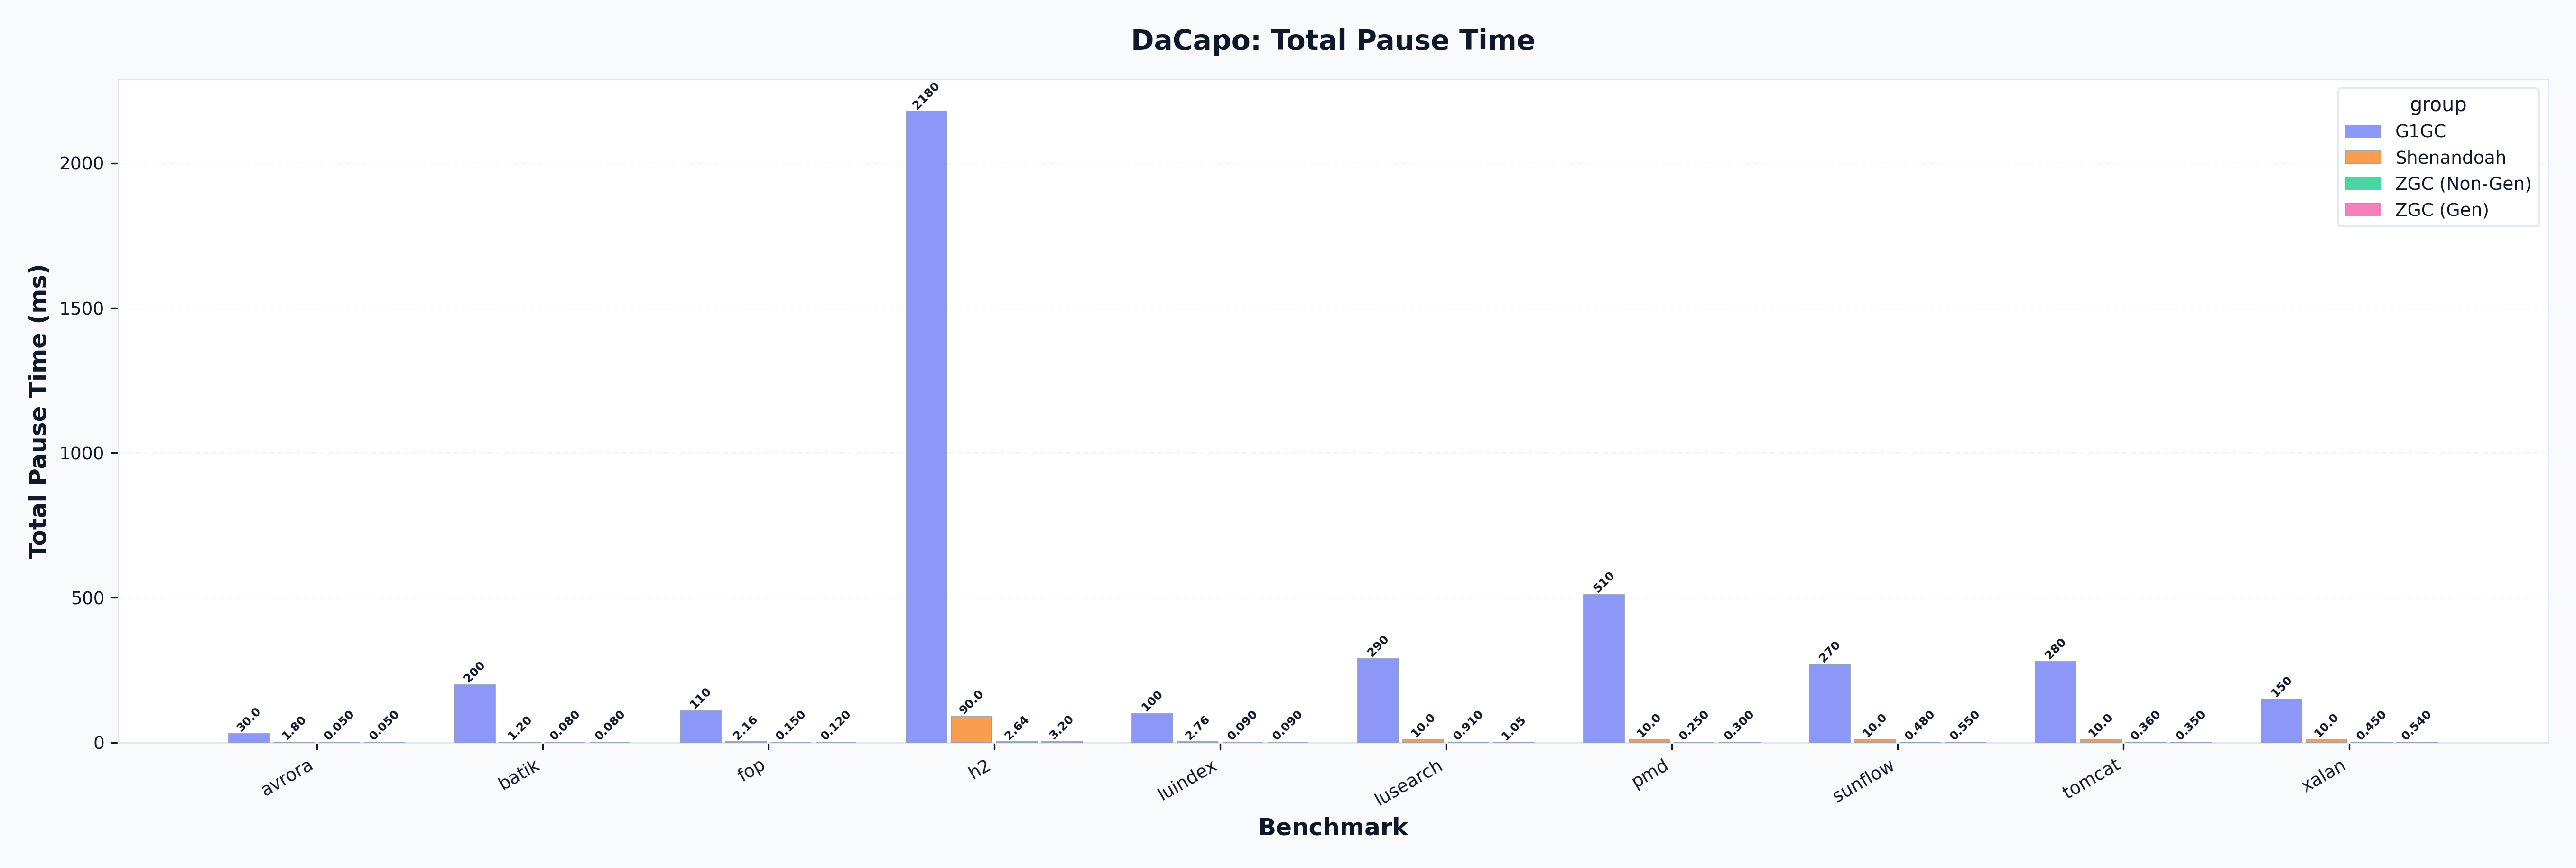
\includegraphics[width=\linewidth]{graphs/dacapo/dacapo_accumPause.png}
\caption{Accumulated Pause}
\end{subfigure} &
\begin{subfigure}{0.45\textwidth}
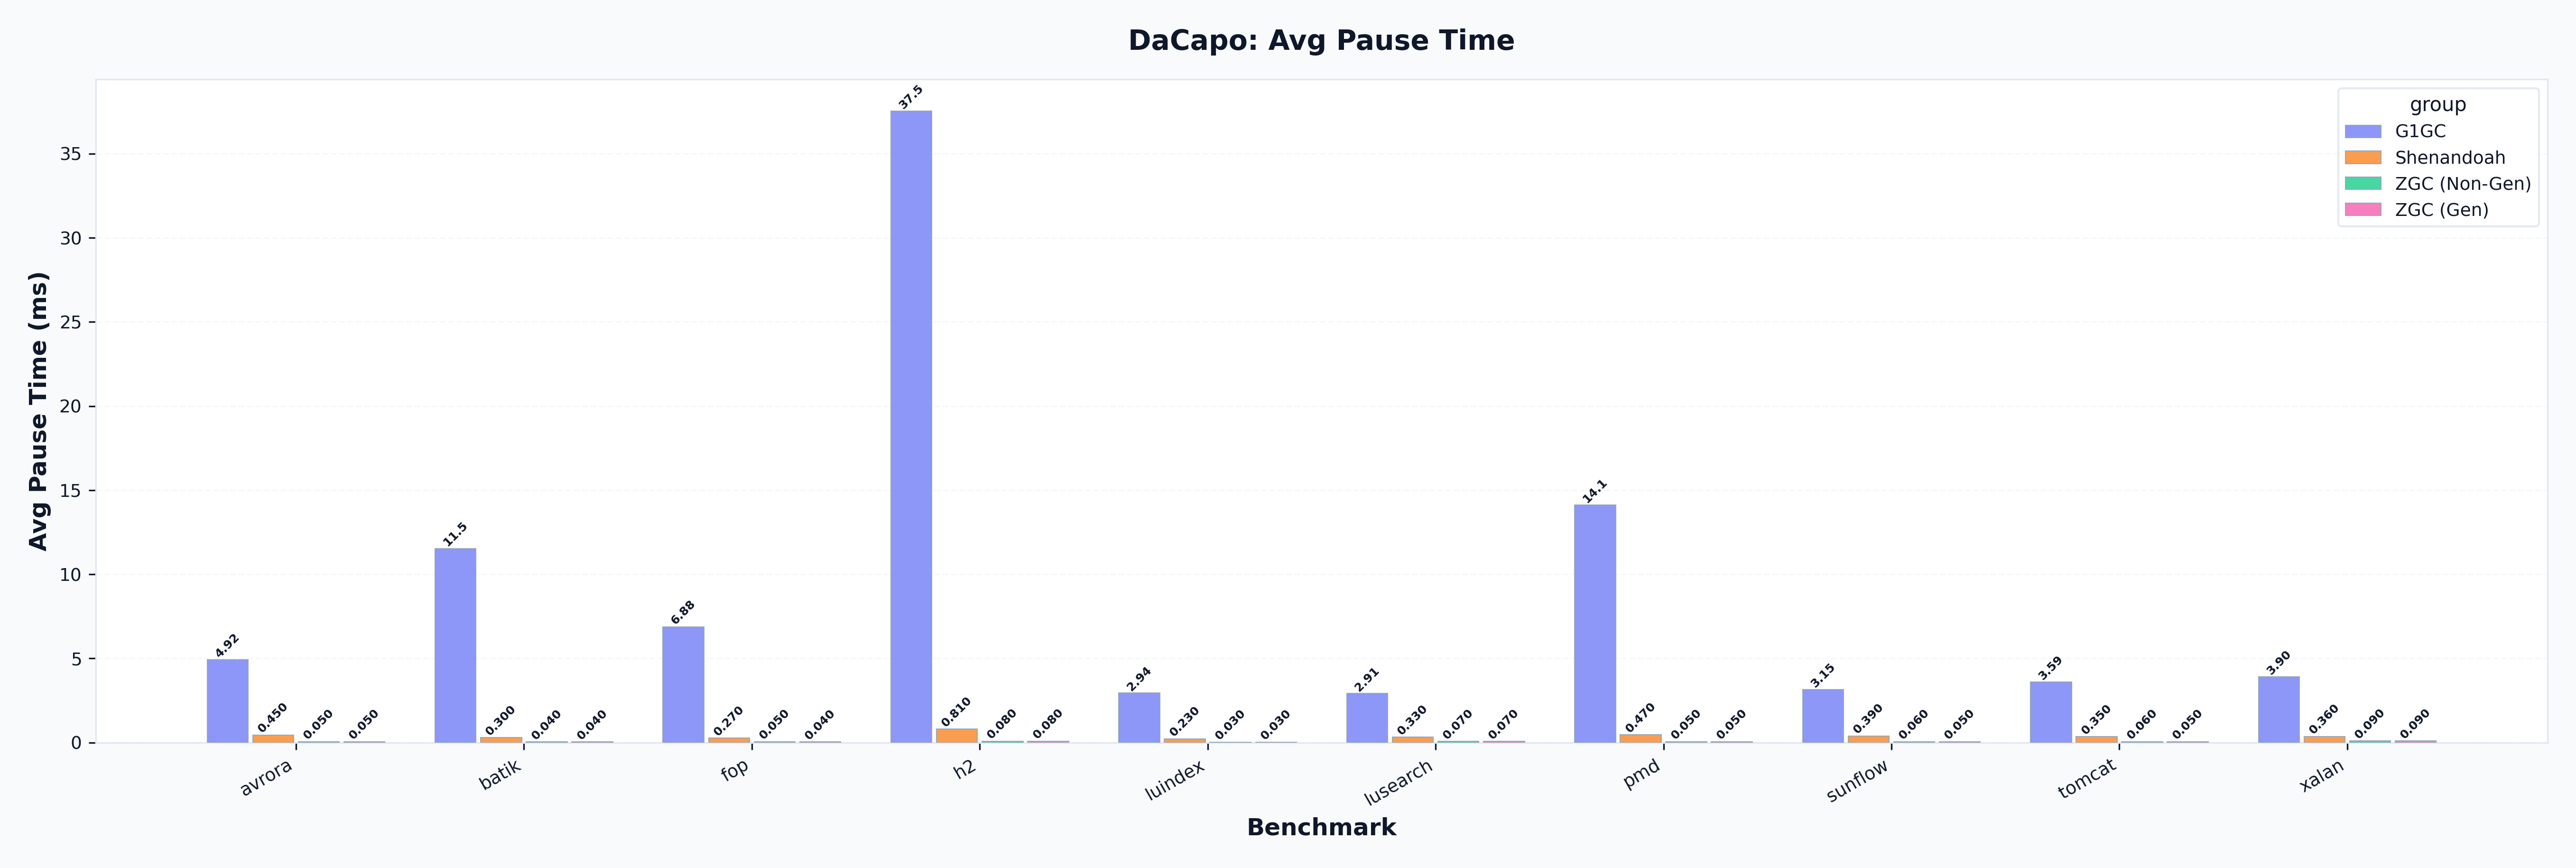
\includegraphics[width=\linewidth]{graphs/dacapo/dacapo_avgPause.png}
\caption{Average Pause}
\end{subfigure} \\

\begin{subfigure}{0.45\textwidth}
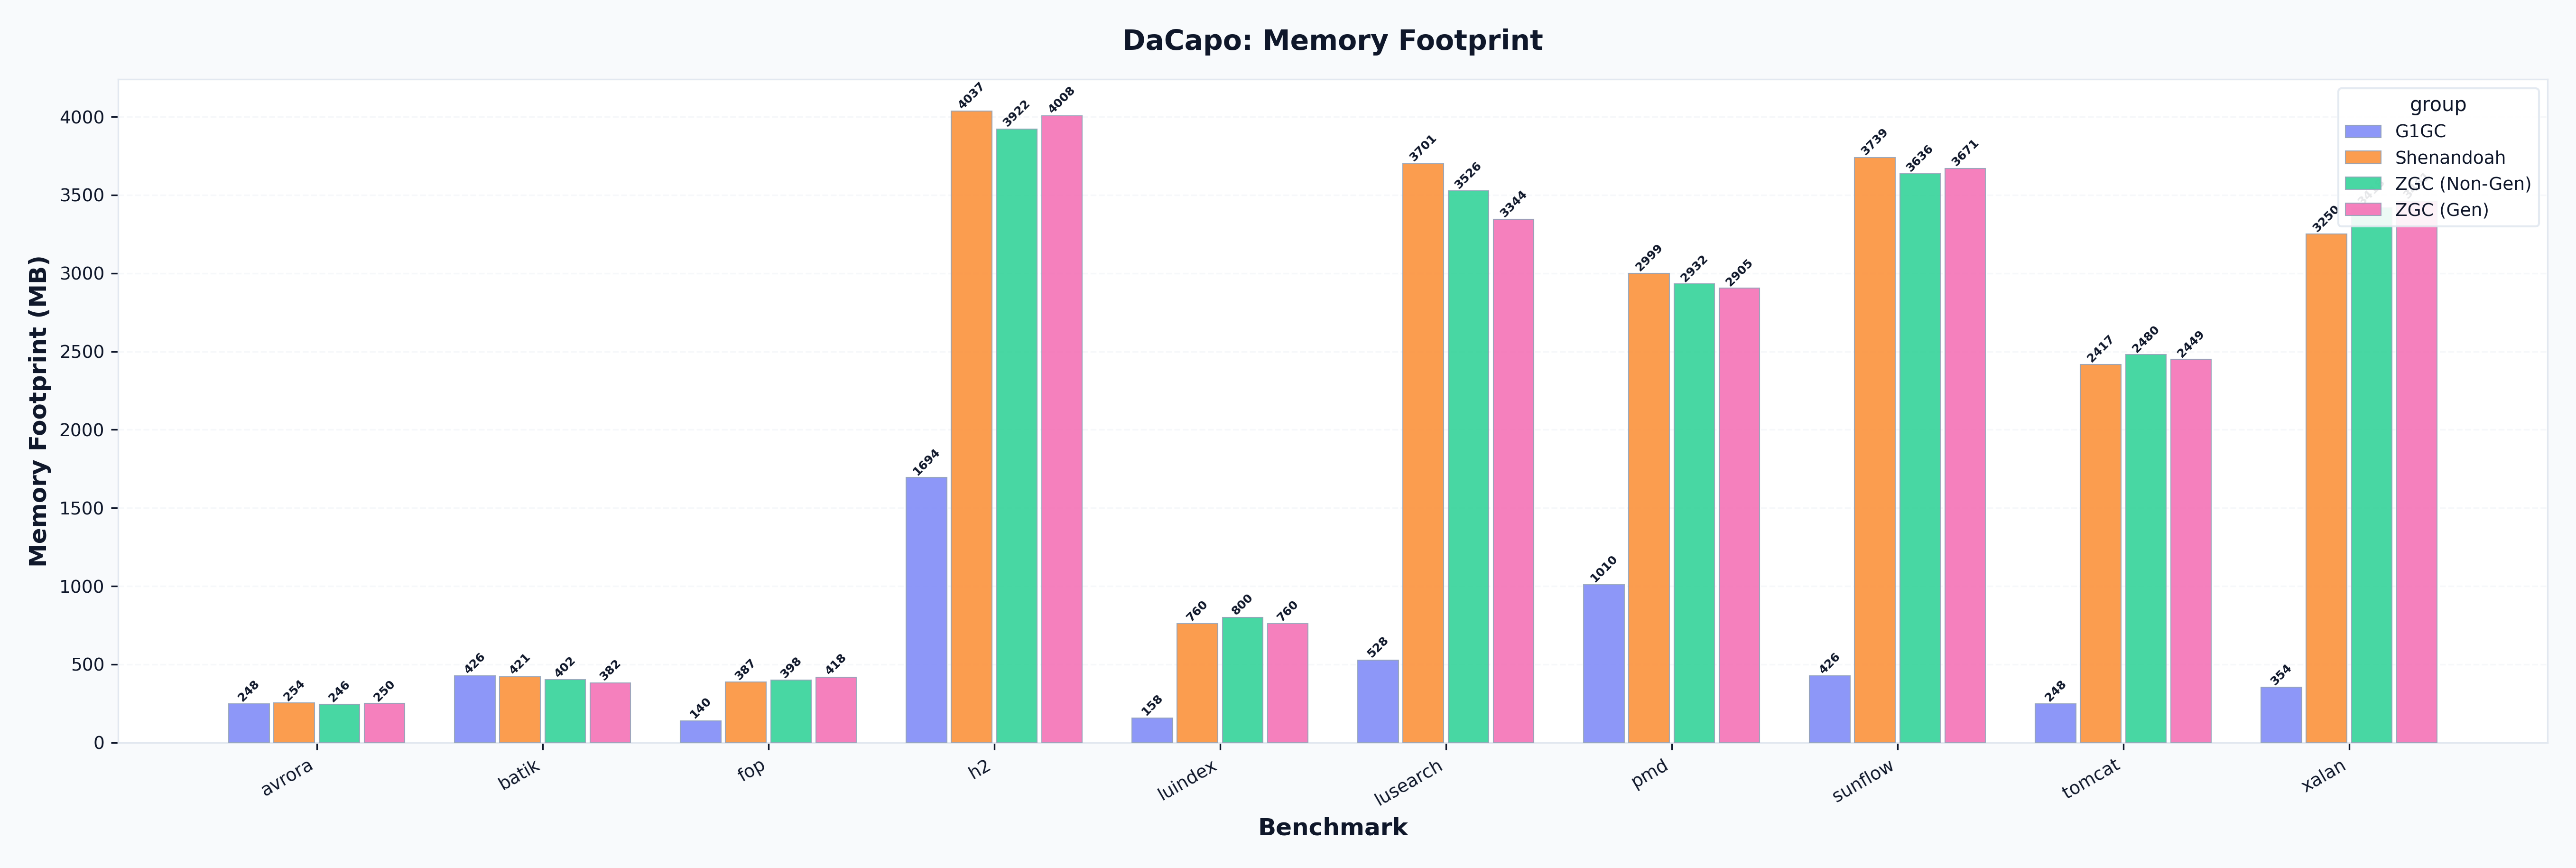
\includegraphics[width=\linewidth]{graphs/dacapo/dacapo_footprint.png}
\caption{Footprint}
\end{subfigure} &
\begin{subfigure}{0.45\textwidth}
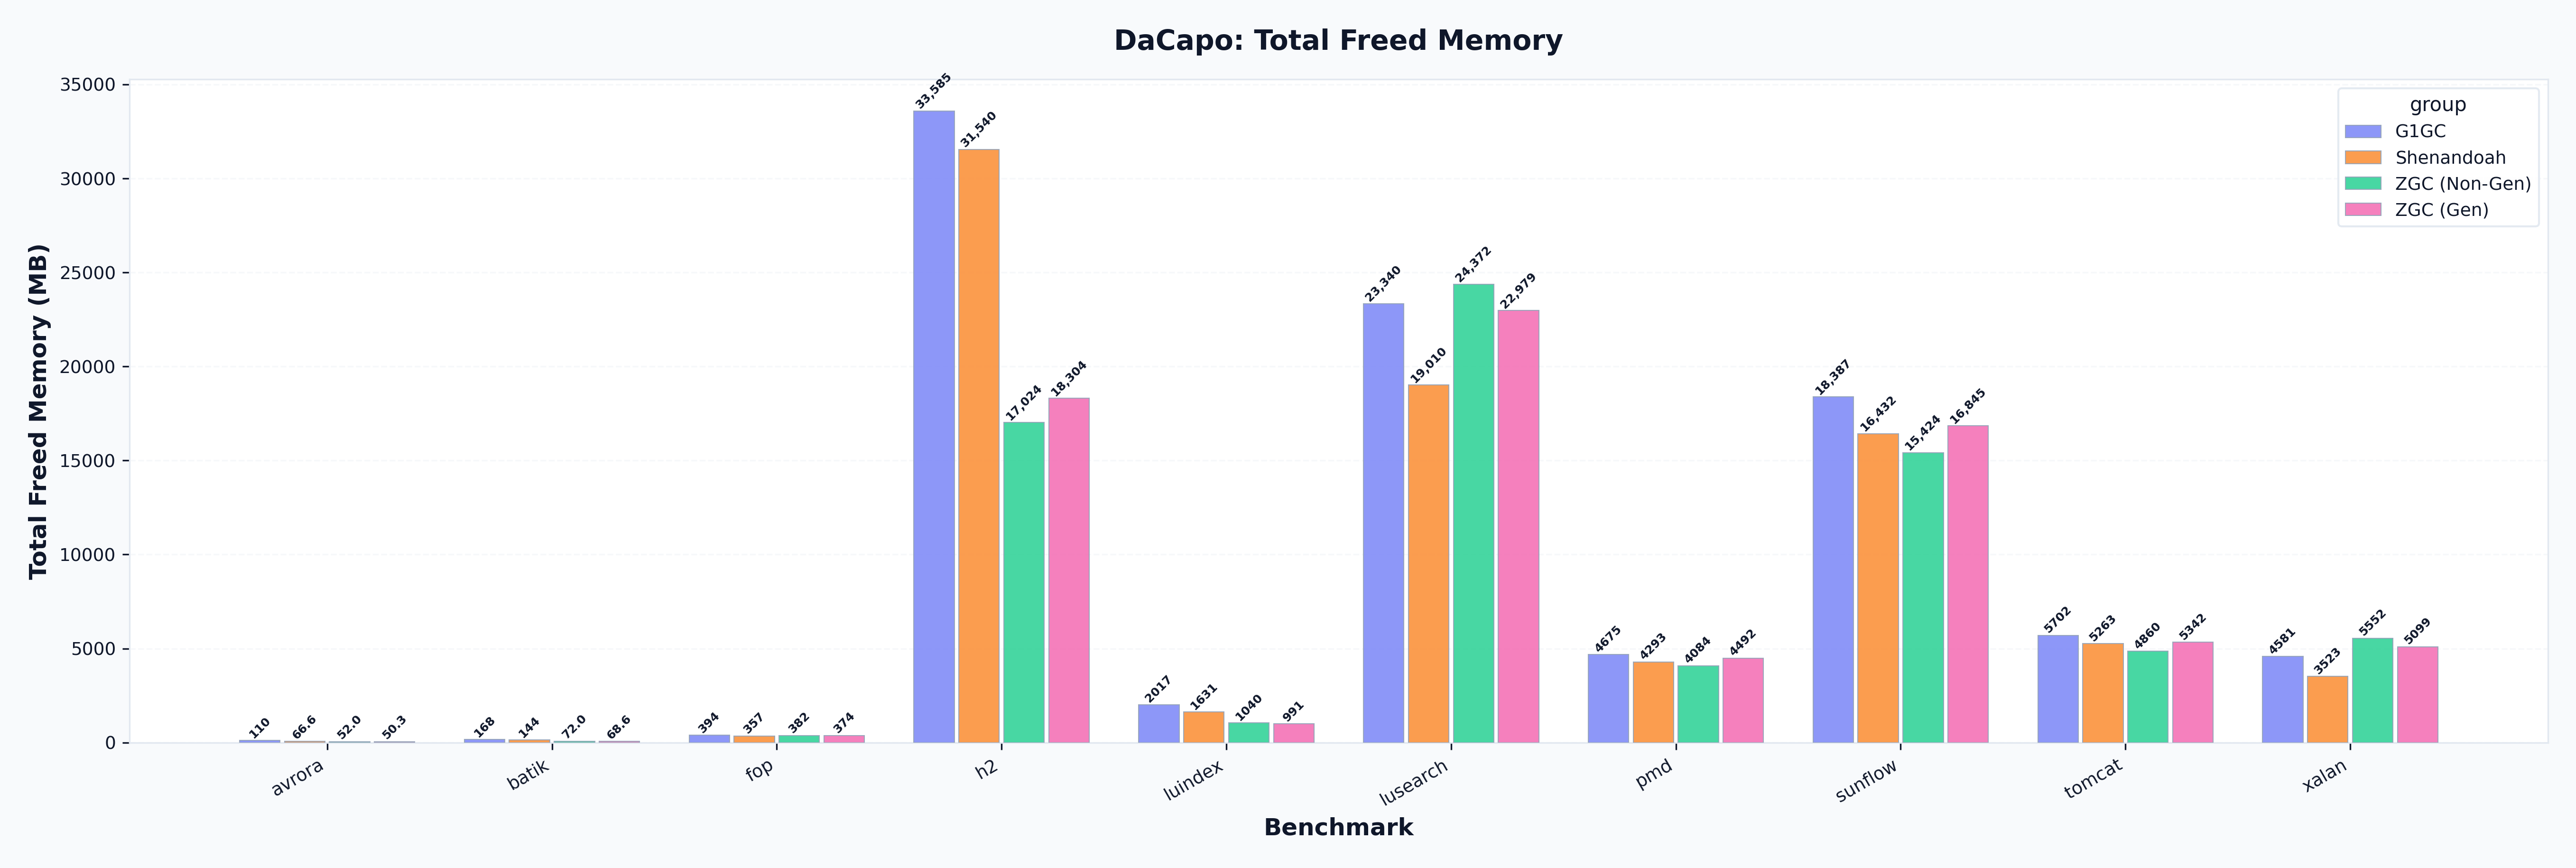
\includegraphics[width=\linewidth]{graphs/dacapo/dacapo_freedMemory.png}
\caption{Freed Memory}
\end{subfigure} \\

\begin{subfigure}{0.45\textwidth}
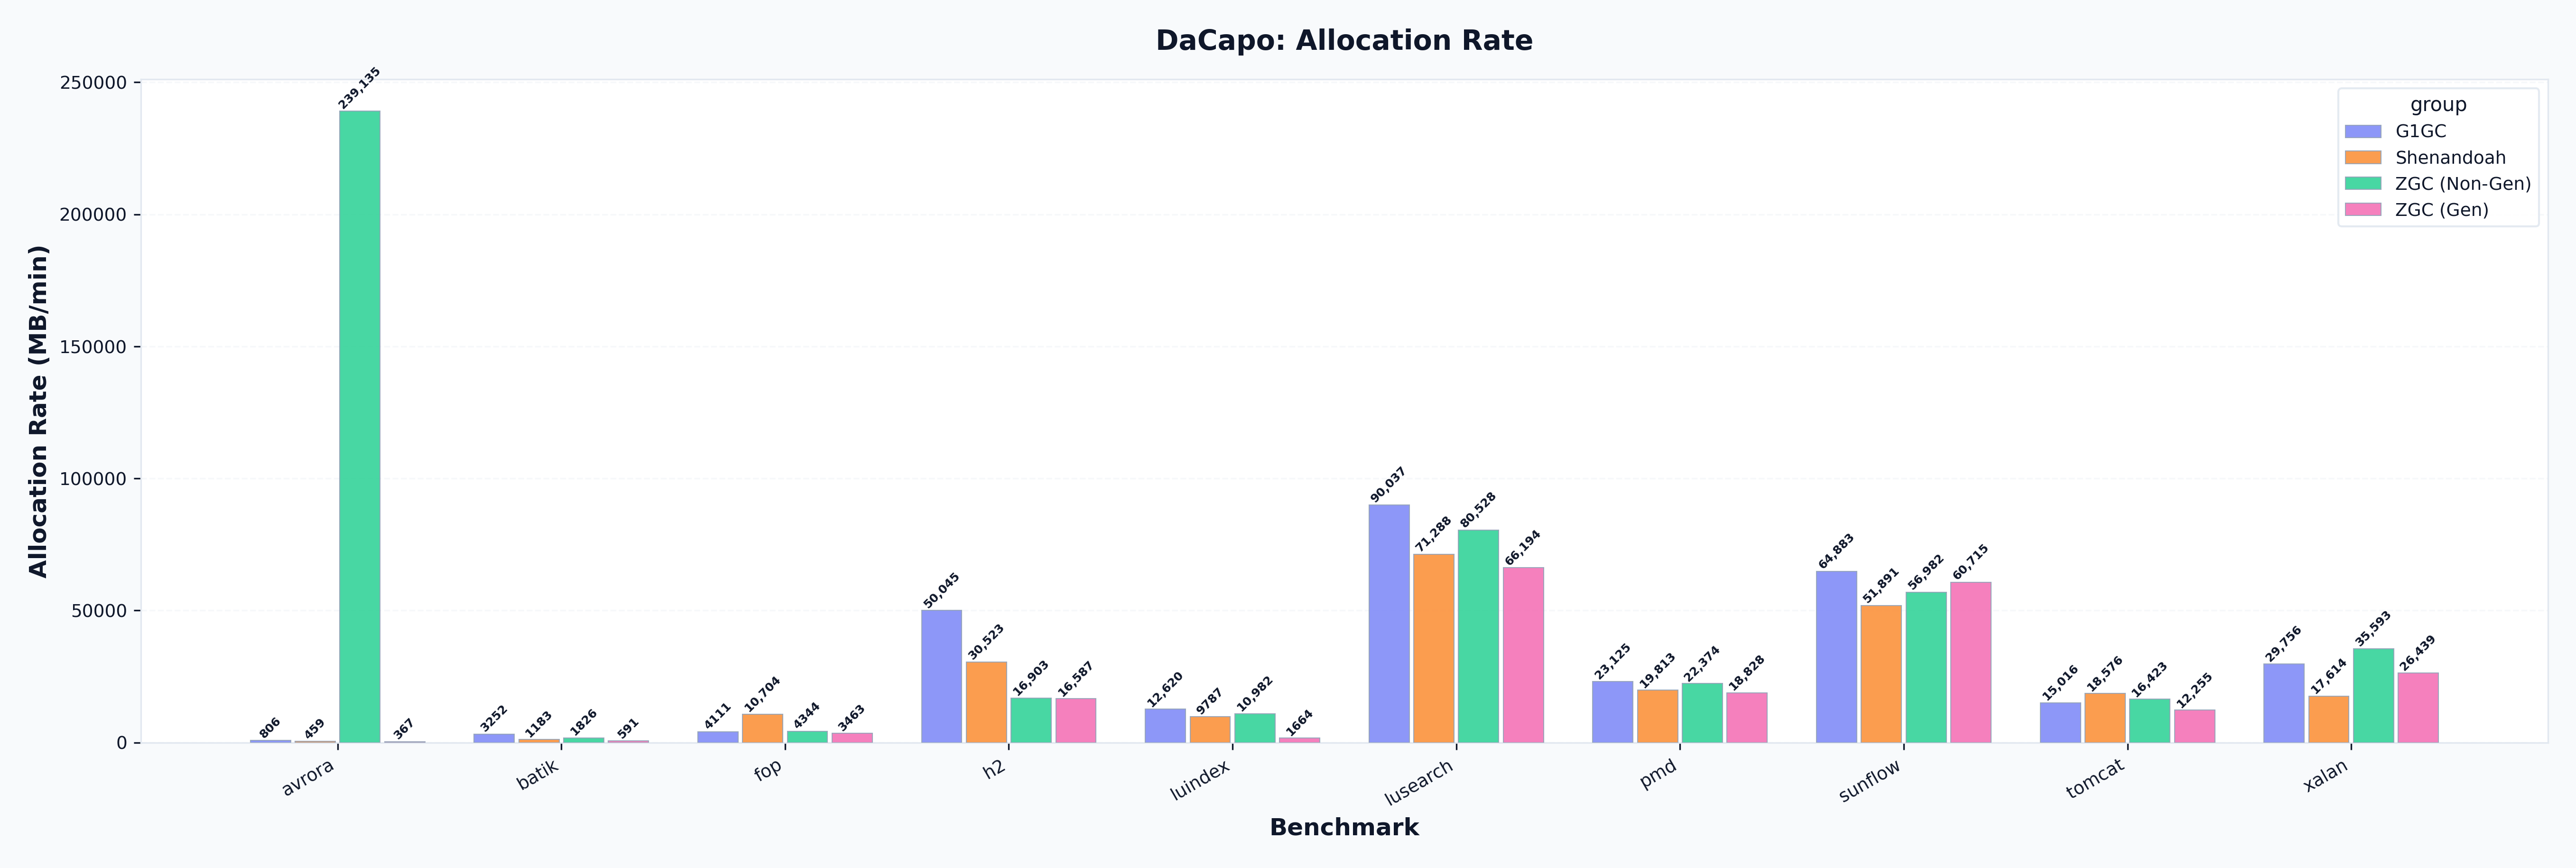
\includegraphics[width=\linewidth]{graphs/dacapo/dacapo_freedMemoryPerMin.png}
\caption{Freed Memory per Min}
\end{subfigure} &
\begin{subfigure}{0.45\textwidth}
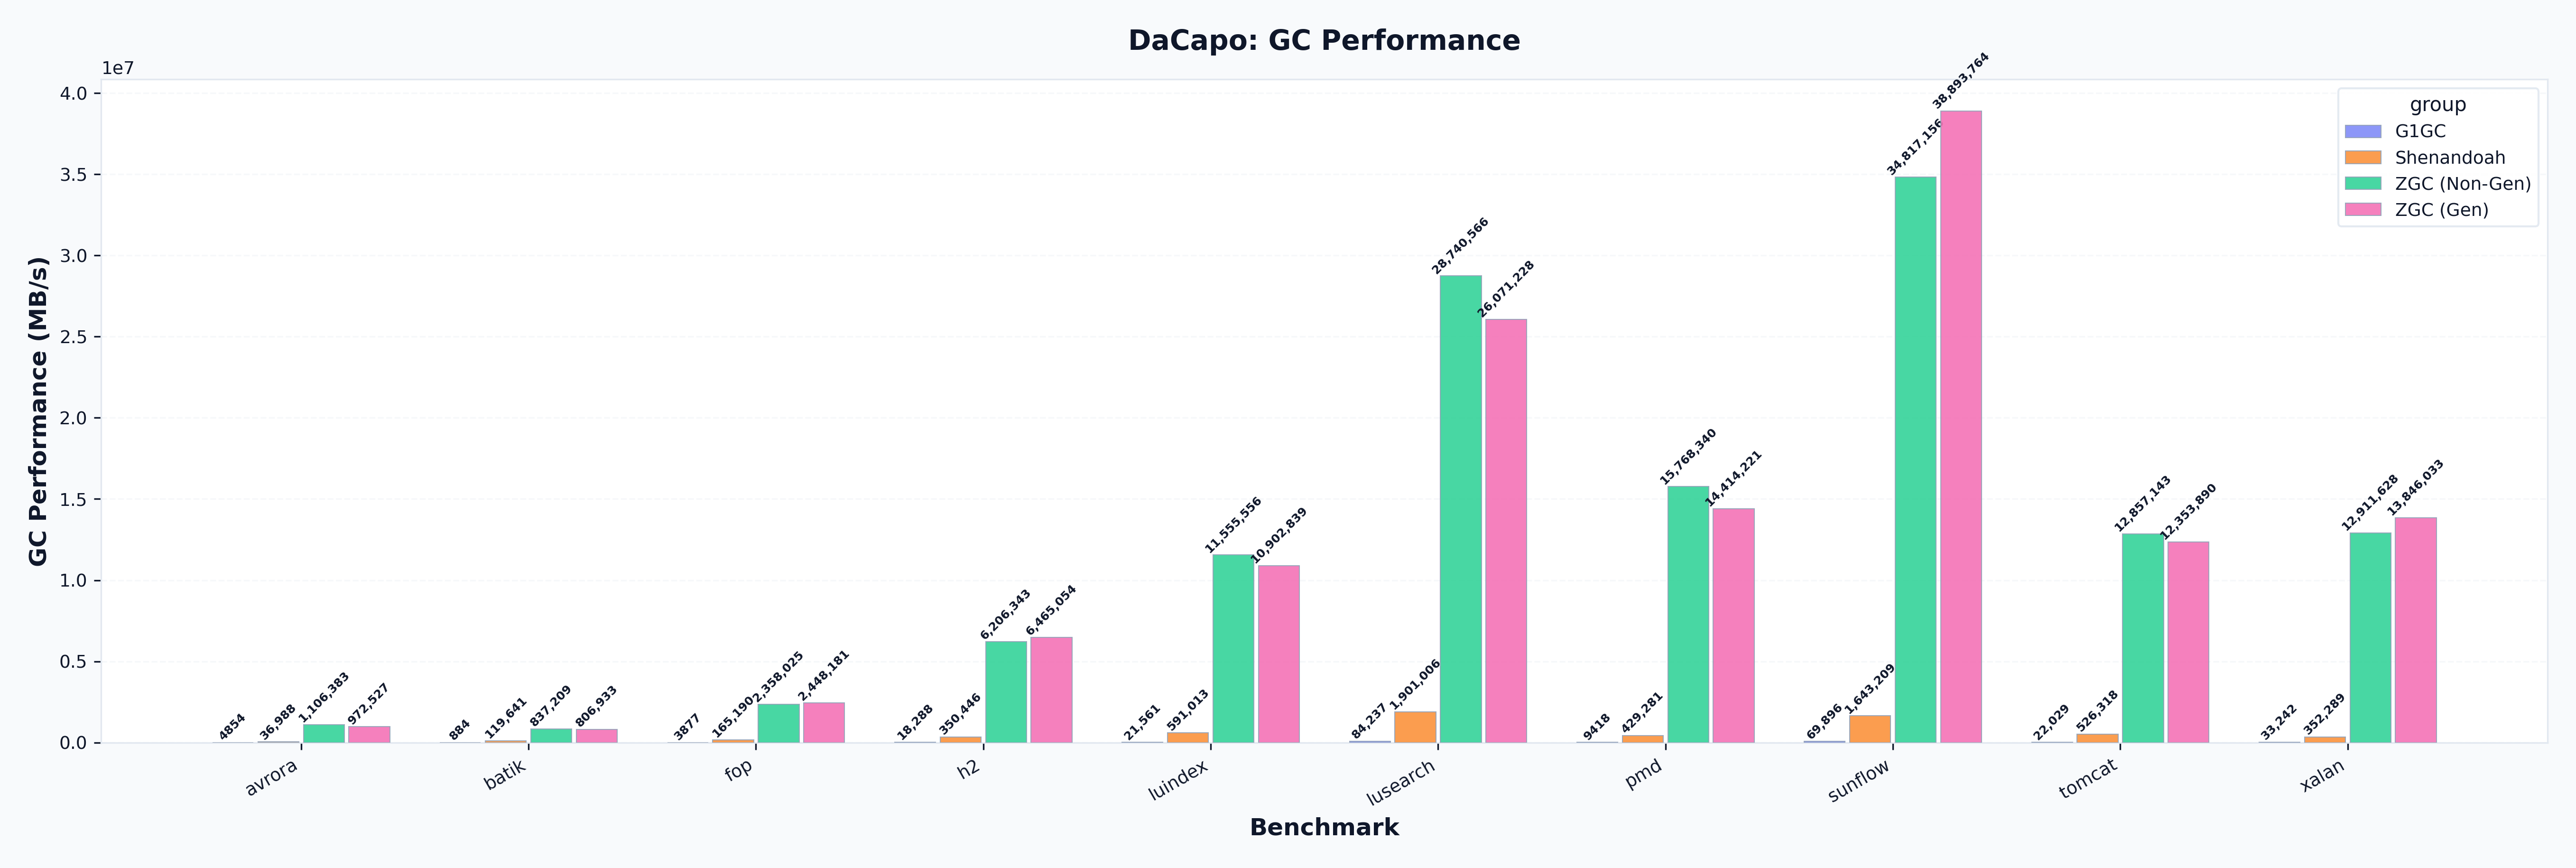
\includegraphics[width=\linewidth]{graphs/dacapo/dacapo_gcPerformance.png}
\caption{GC Performance}
\end{subfigure} \\

\begin{subfigure}{0.45\textwidth}
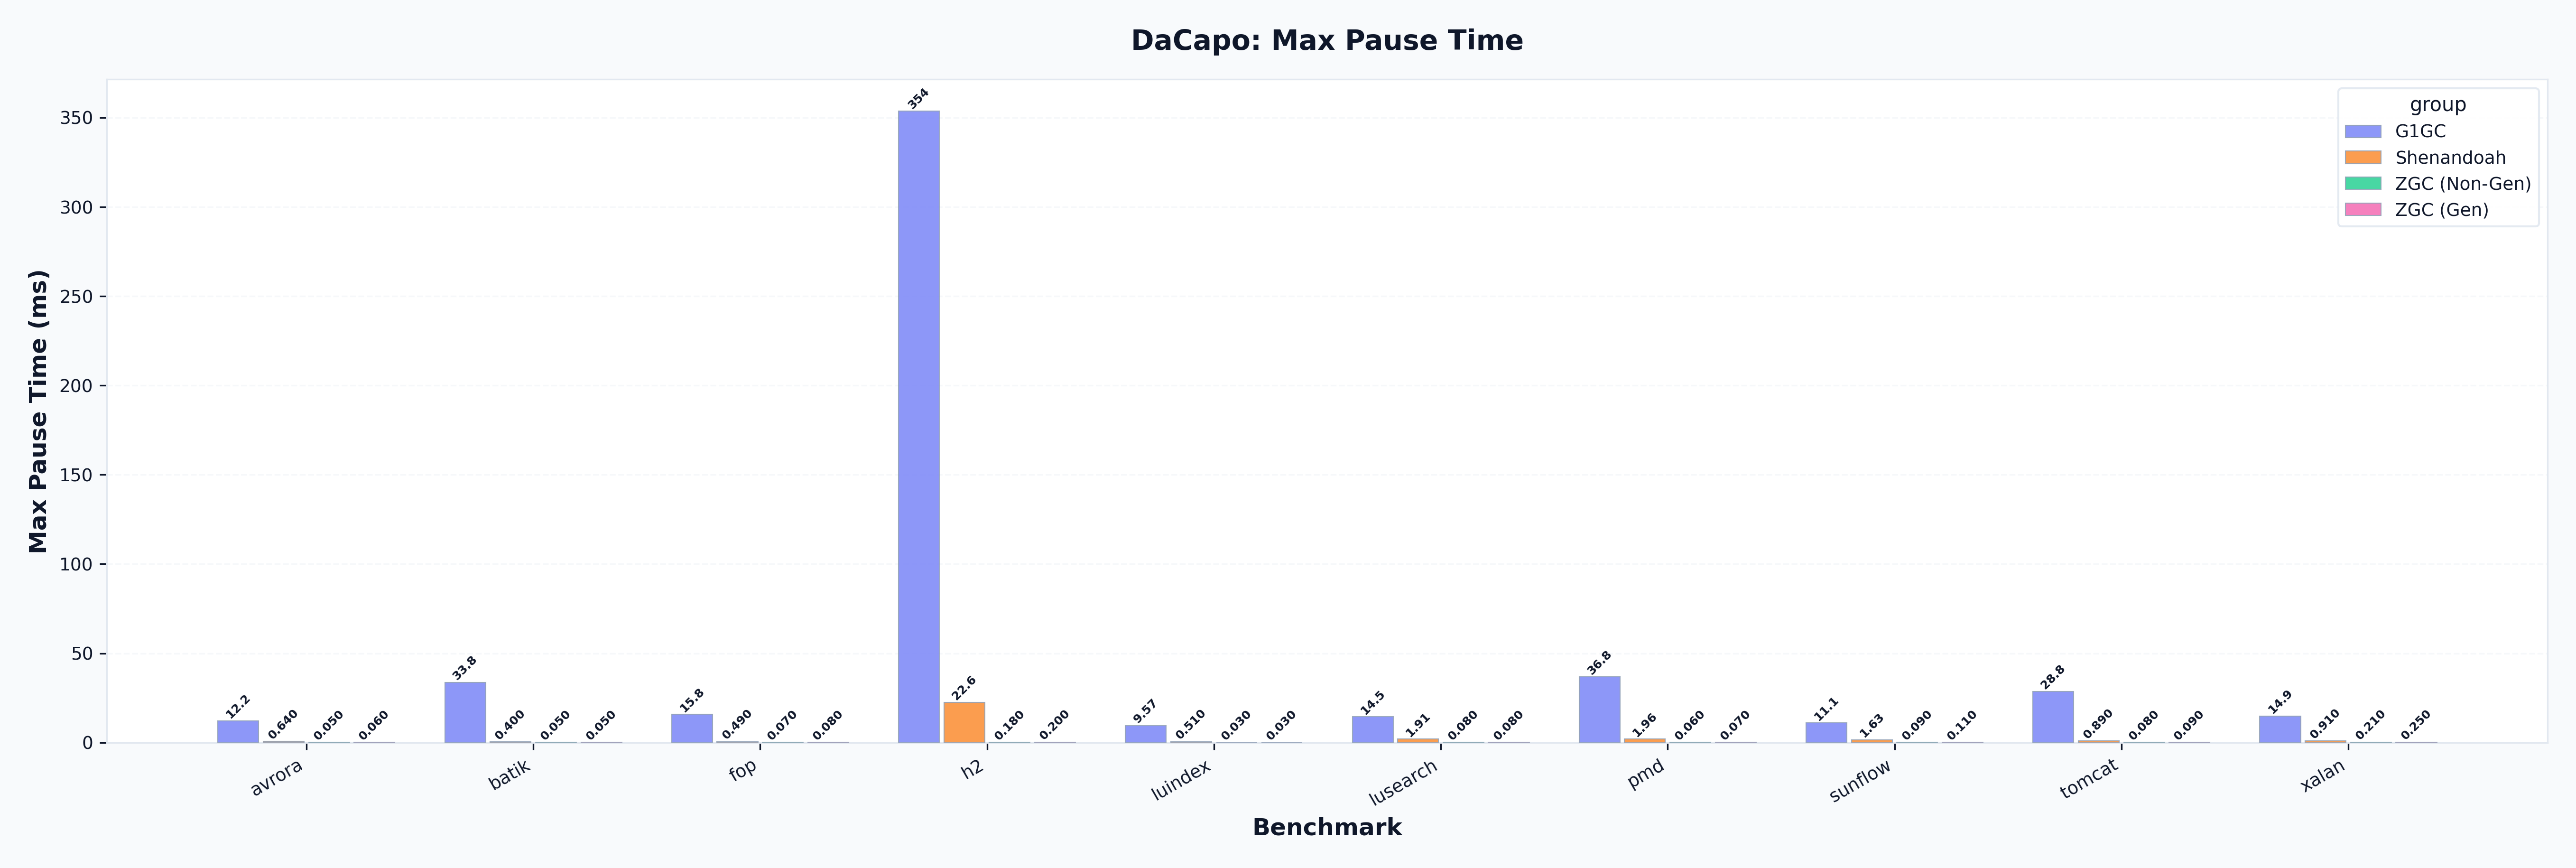
\includegraphics[width=\linewidth]{graphs/dacapo/dacapo_maxPause.png}
\caption{Max Pause}
\end{subfigure} &
\begin{subfigure}{0.45\textwidth}
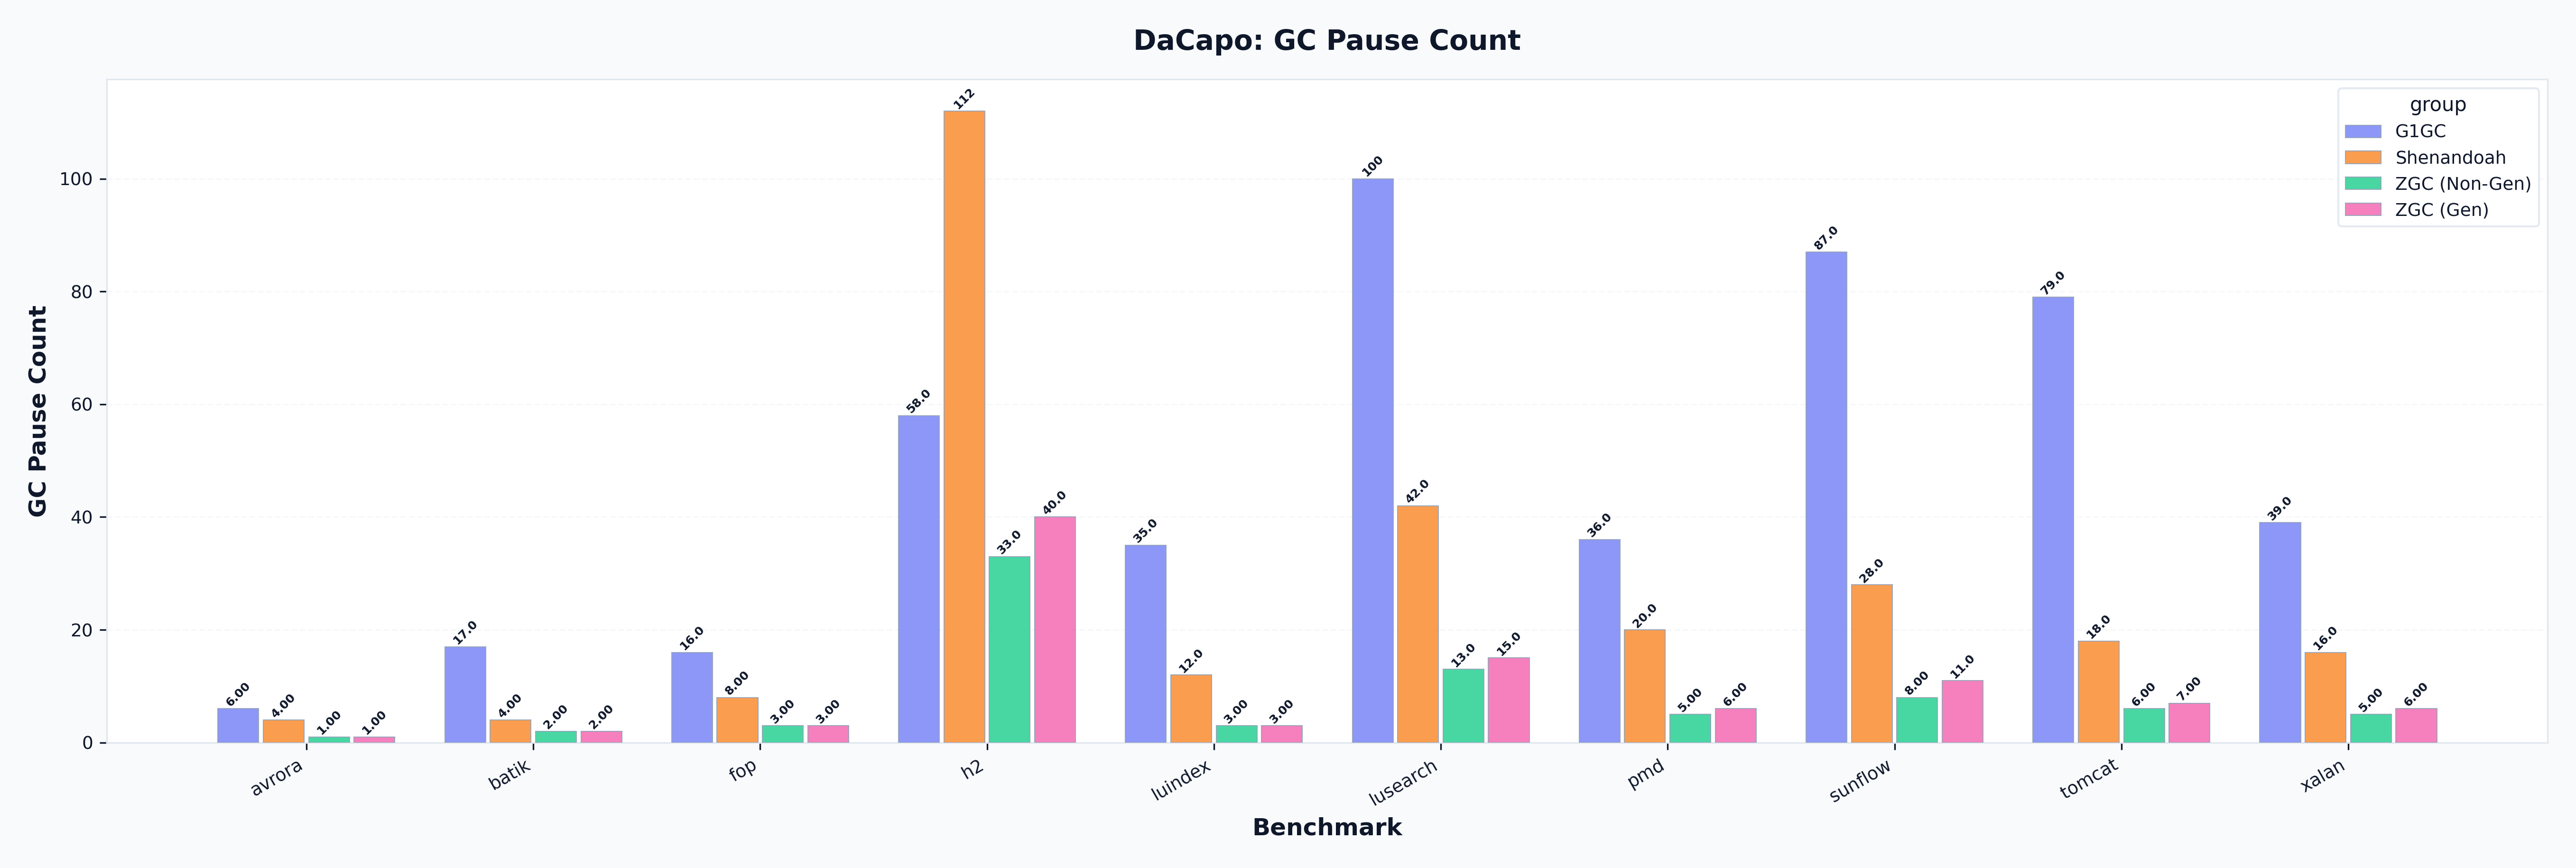
\includegraphics[width=\linewidth]{graphs/dacapo/dacapo_pauseCount.png}
\caption{Pause Count}
\end{subfigure} \\

\begin{subfigure}{0.45\textwidth}
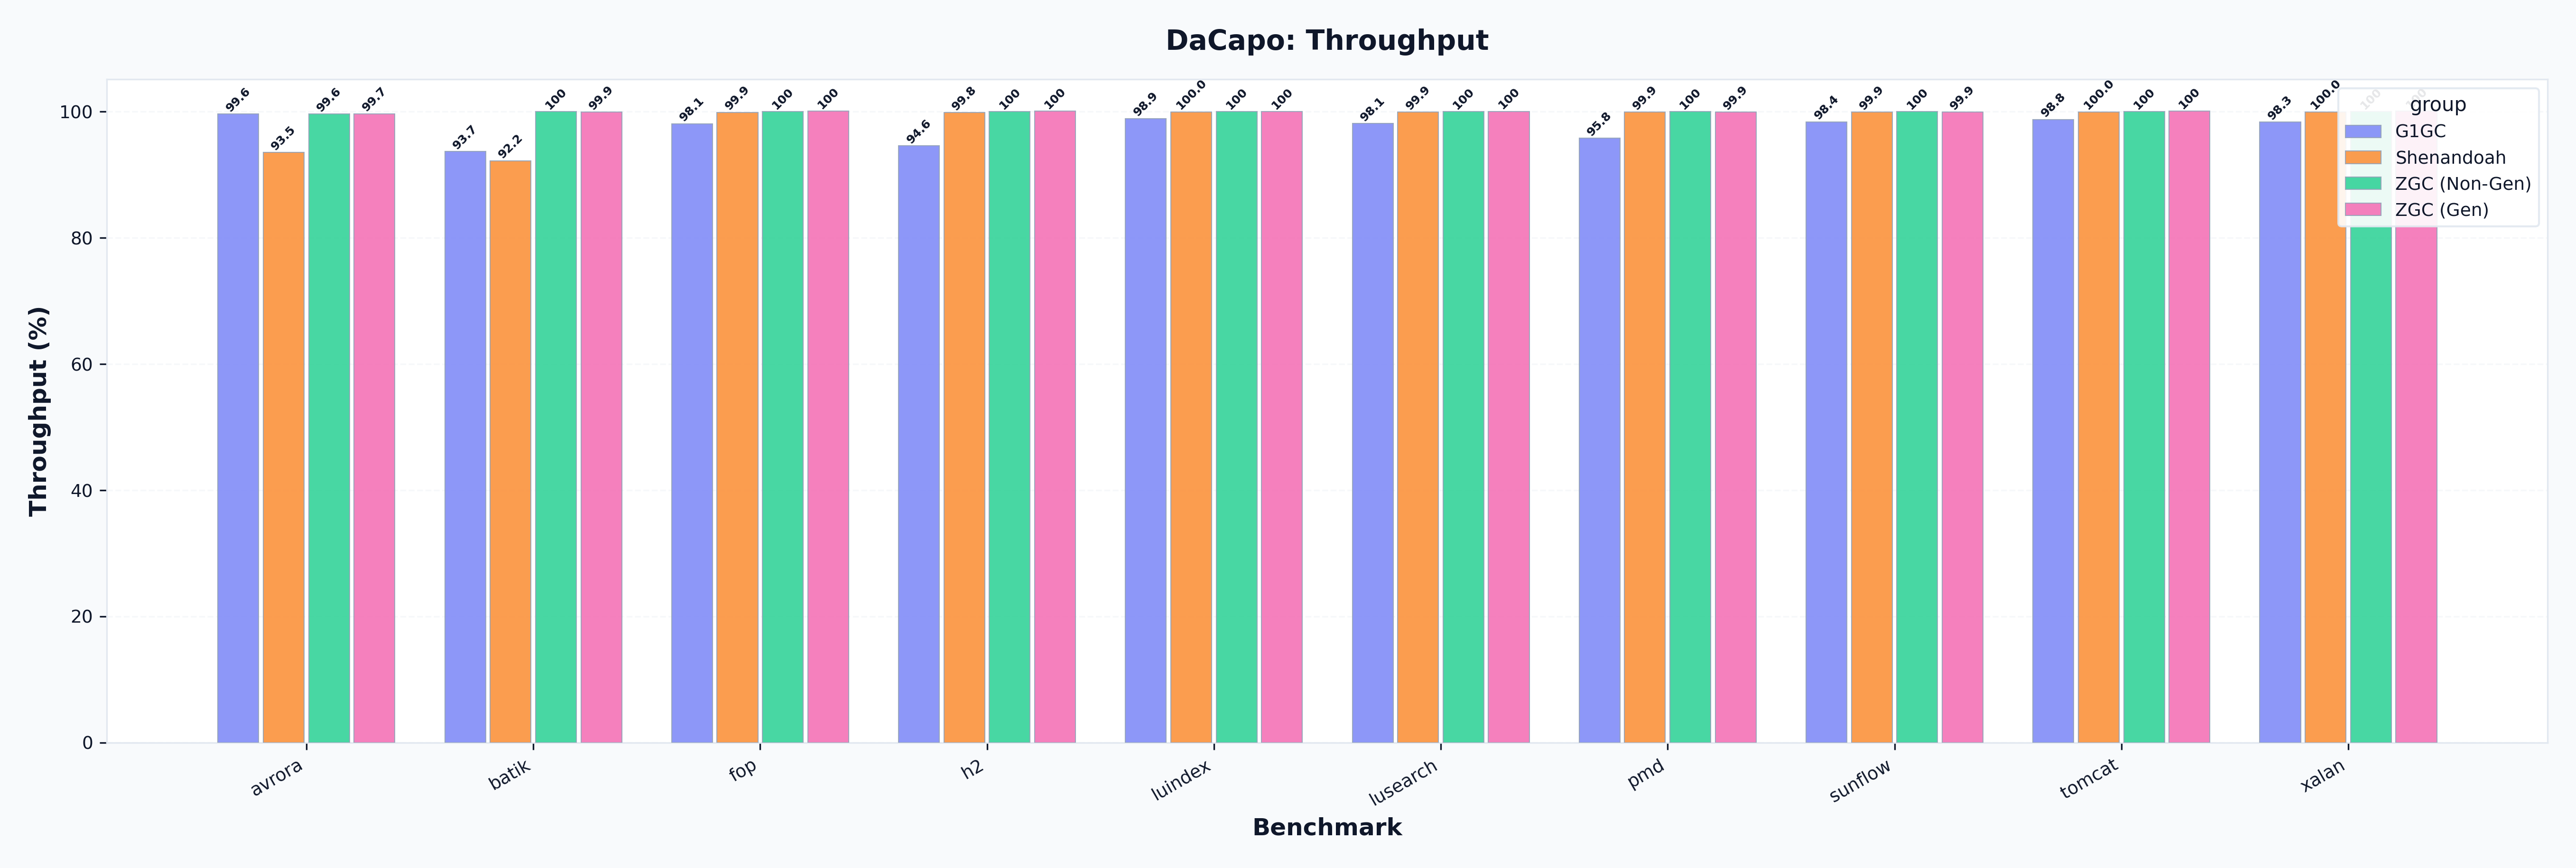
\includegraphics[width=\linewidth]{graphs/dacapo/dacapo_throughput.png}
\caption{Throughput}
\end{subfigure} &
\begin{subfigure}{0.45\textwidth}
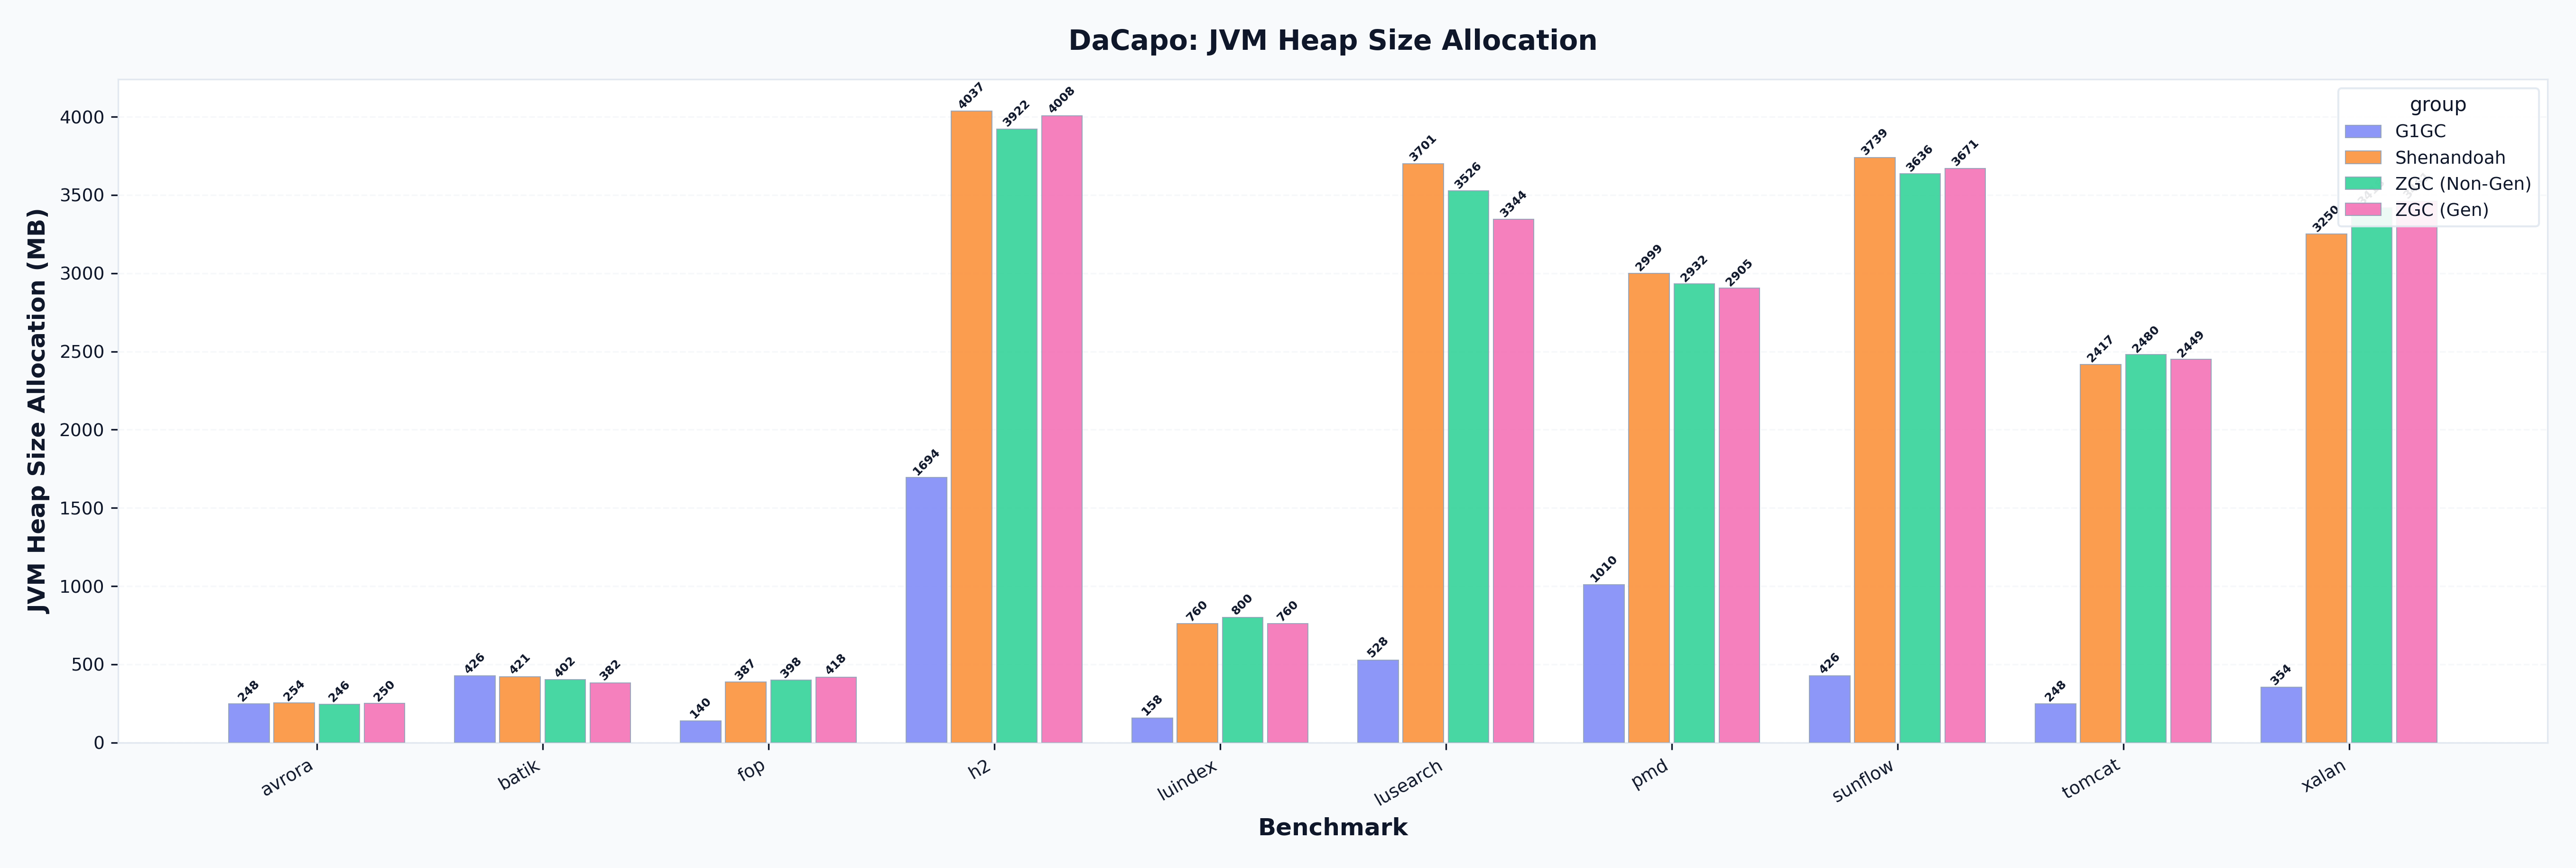
\includegraphics[width=\linewidth]{graphs/dacapo/dacapo_totalHeapAllocMax.png}
\caption{Total Heap Alloc Max}
\end{subfigure} \\

\begin{subfigure}{0.45\textwidth}
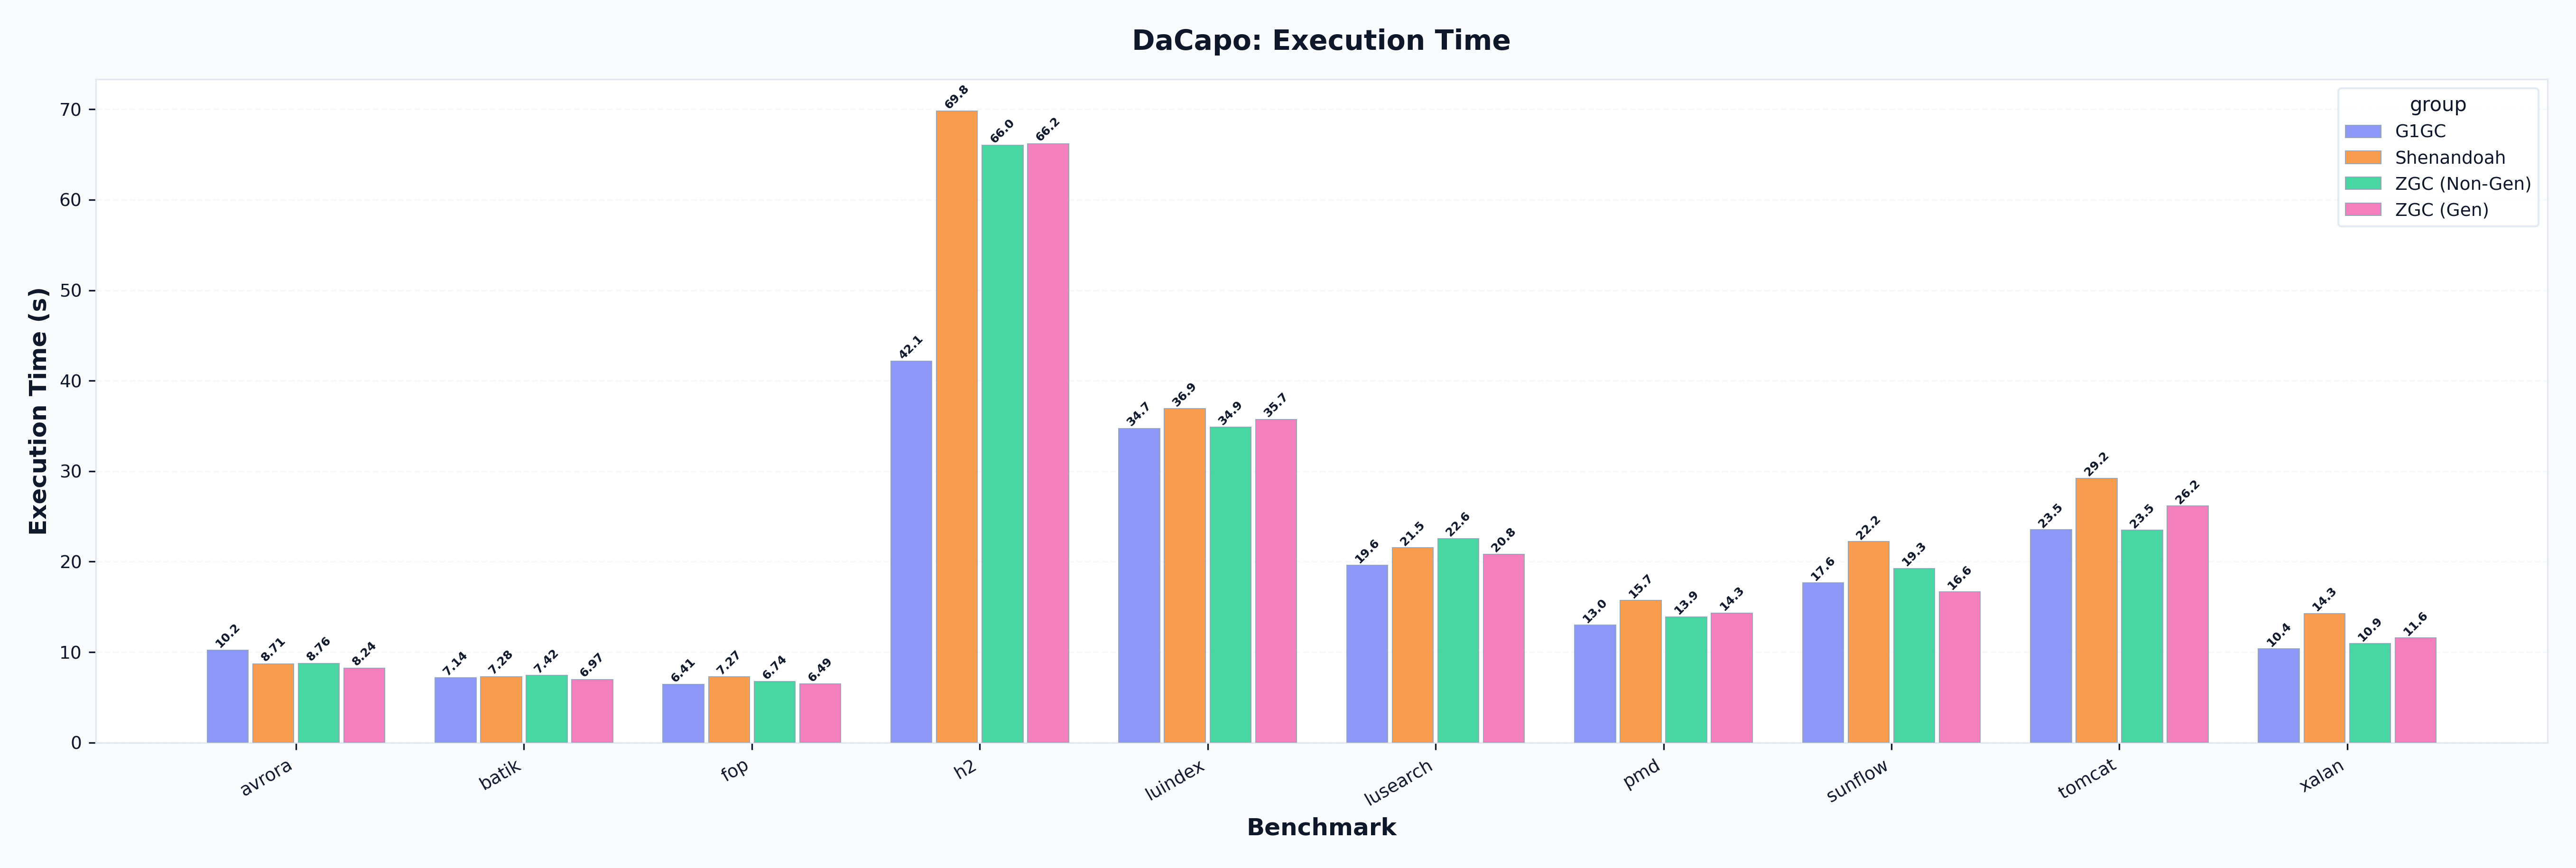
\includegraphics[width=\linewidth]{graphs/dacapo/dacapo_wallTimeSec.png}
\caption{Wall Time (sec)}
\end{subfigure} &
\begin{subfigure}{0.45\textwidth}
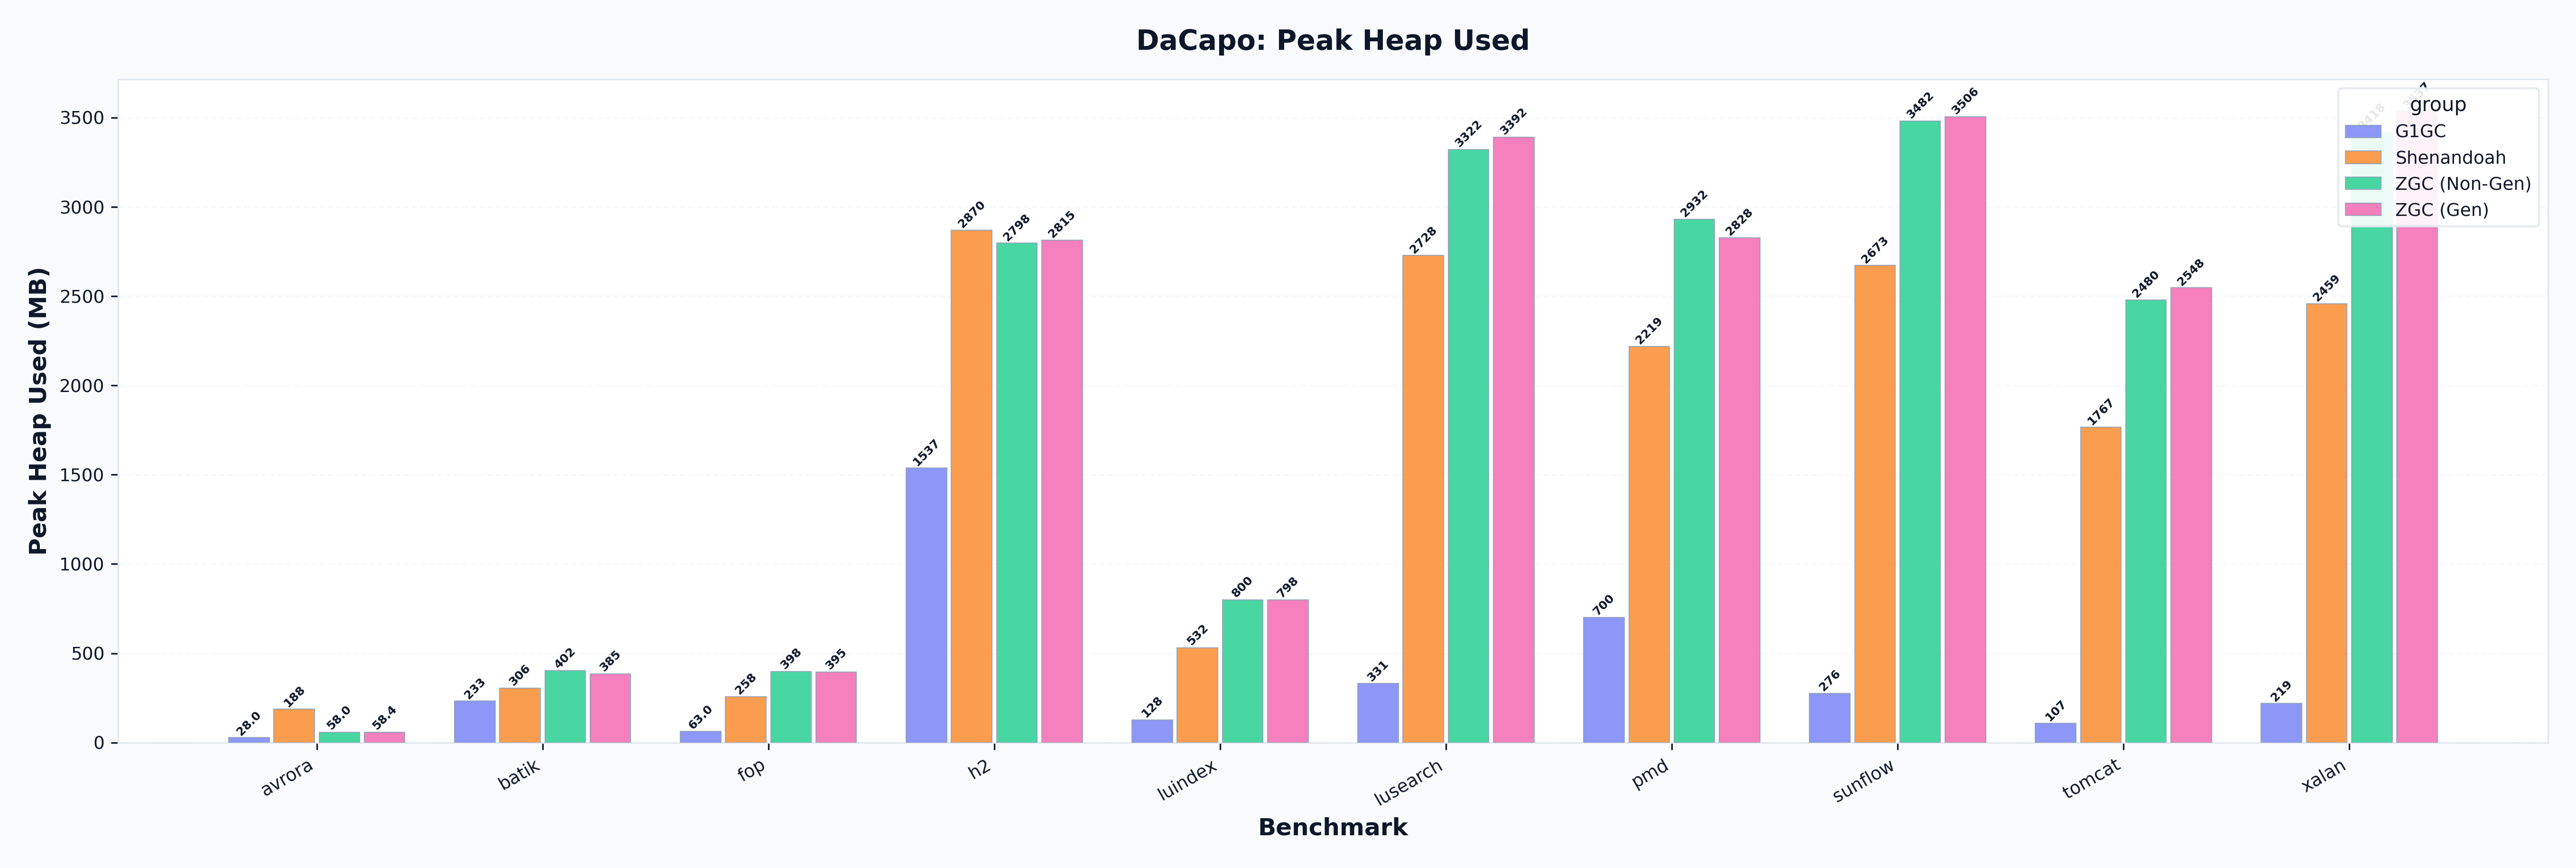
\includegraphics[width=\linewidth]{graphs/dacapo/dacapo_totalHeapUsedMax.png}
\caption{Total Heap Used Max}
\end{subfigure} \\

\end{tabular}

\caption{DaCapo Benchmark Results Across Different Metrics}
\label{fig:dacapo_all_6x2}
\end{figure}



\begin{figure}[h]
\centering

\begin{tabular}{cc}

\begin{subfigure}{0.45\textwidth}
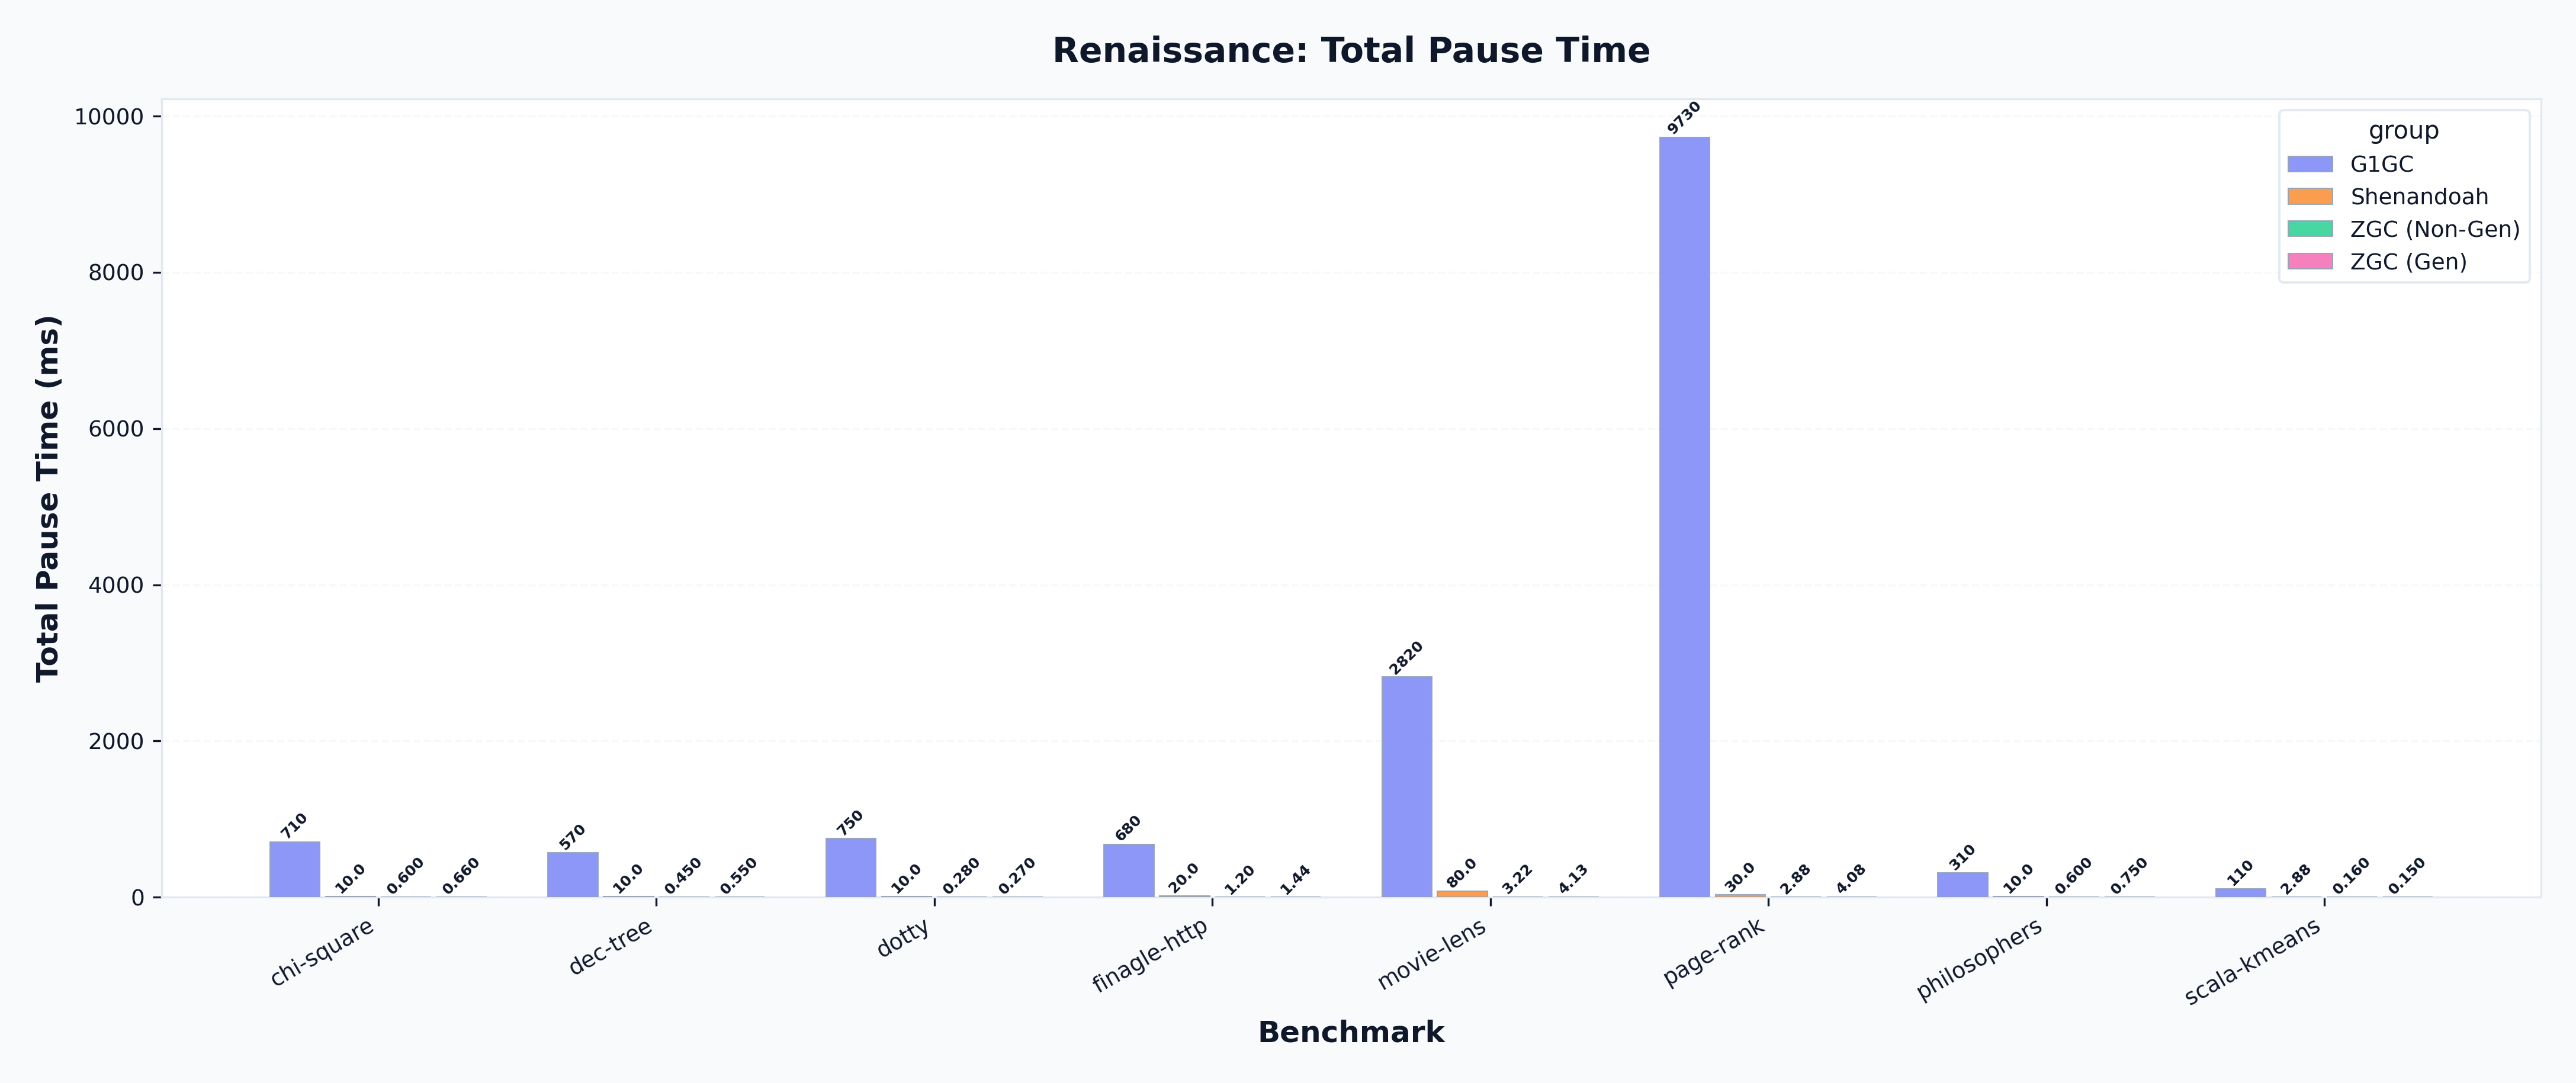
\includegraphics[width=\linewidth]{graphs/renaissance/renaissance_accumPause.png}
\caption{Accumulated Pause}
\end{subfigure} &
\begin{subfigure}{0.45\textwidth}
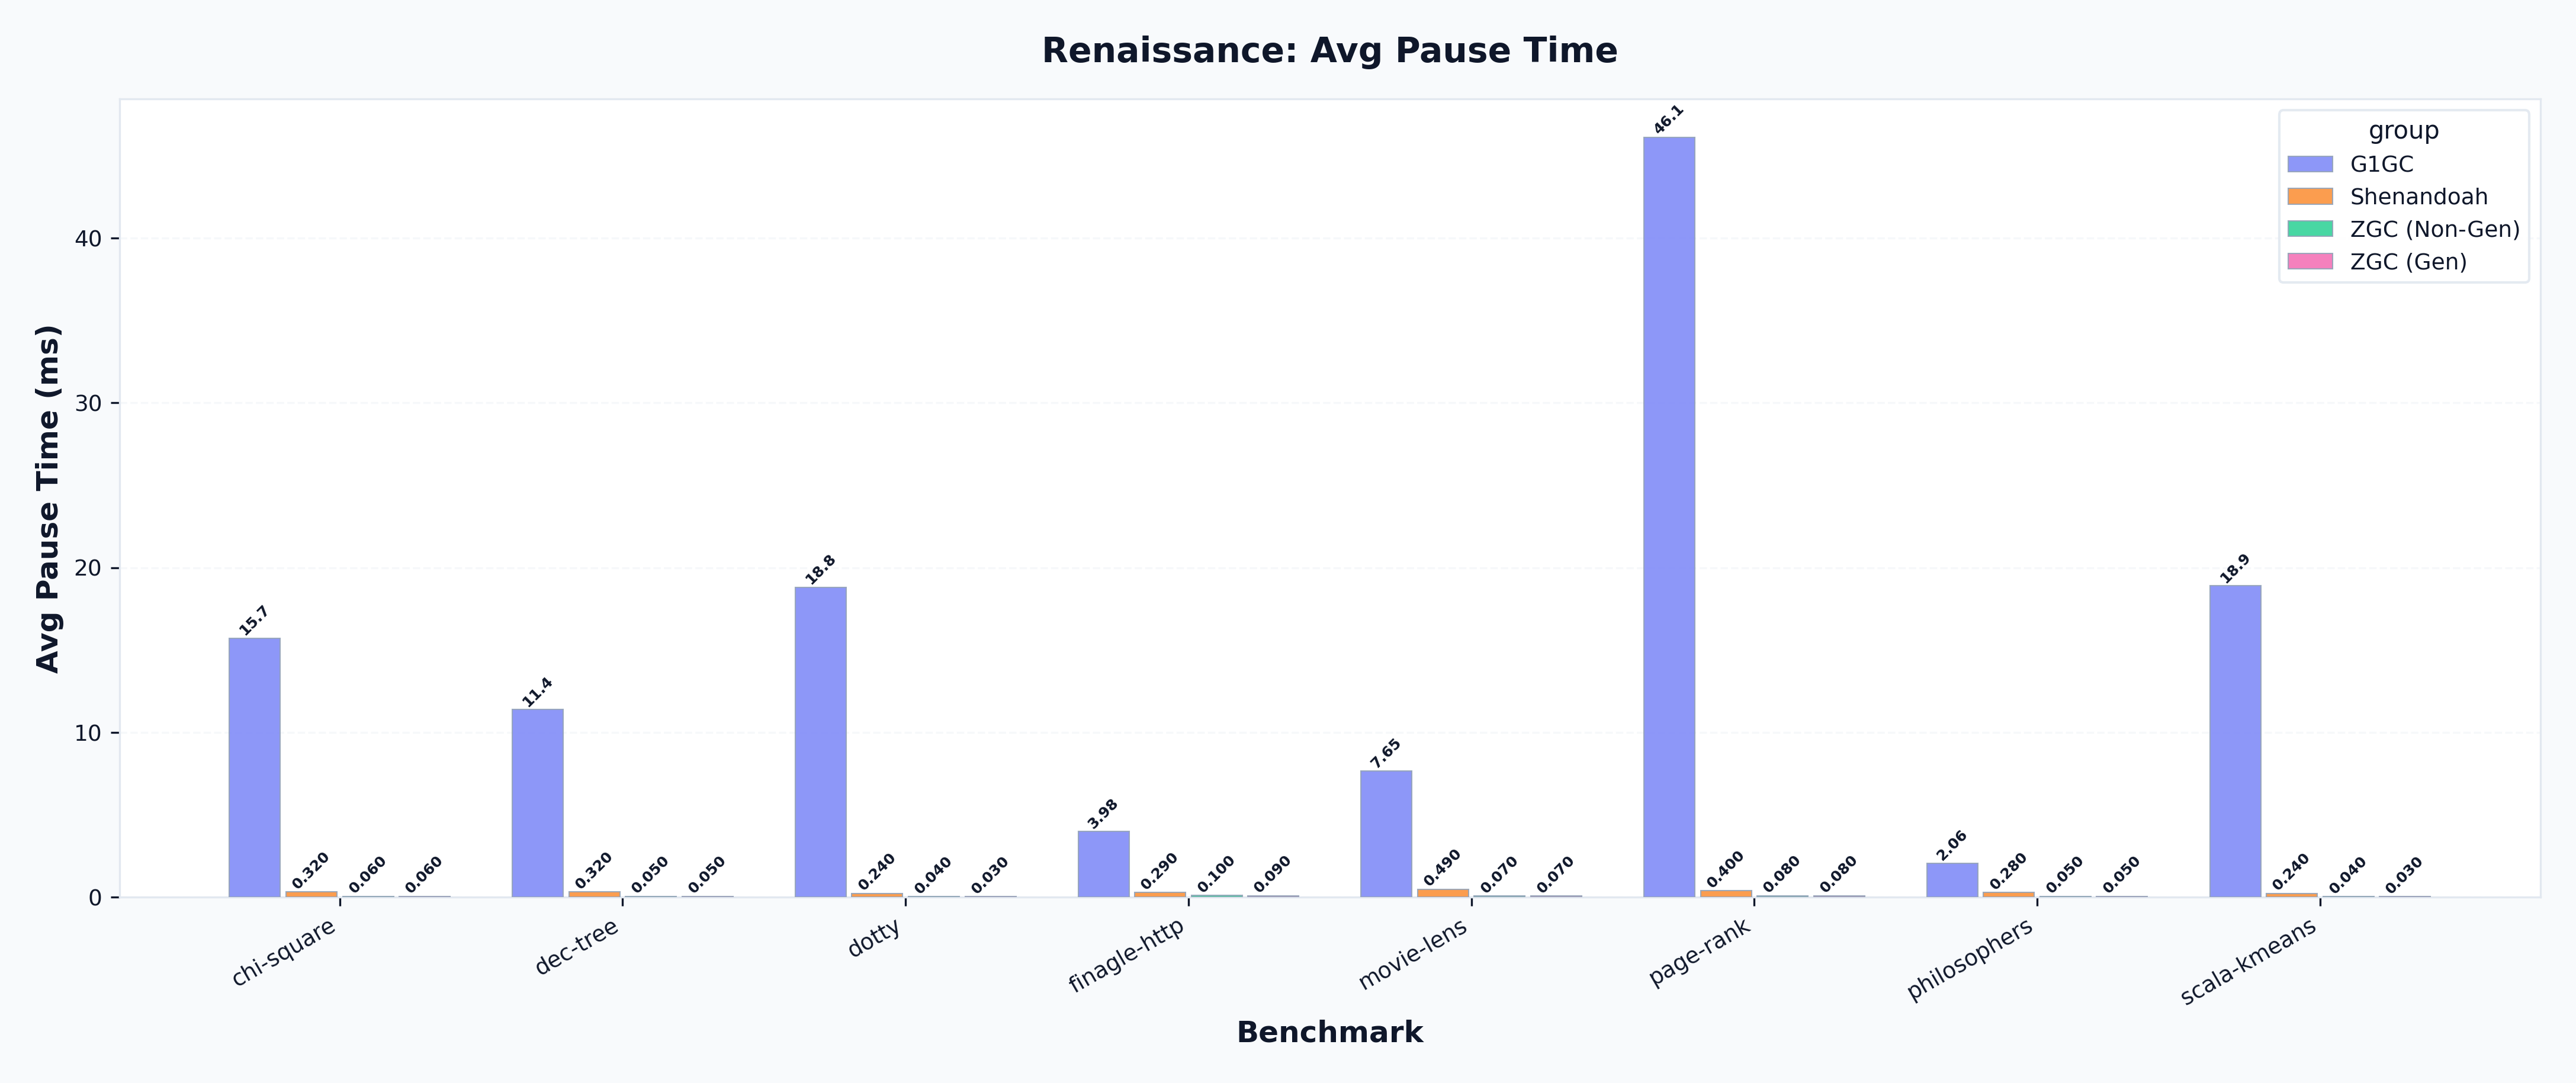
\includegraphics[width=\linewidth]{graphs/renaissance/renaissance_avgPause.png}
\caption{Average Pause}
\end{subfigure} \\

\begin{subfigure}{0.45\textwidth}
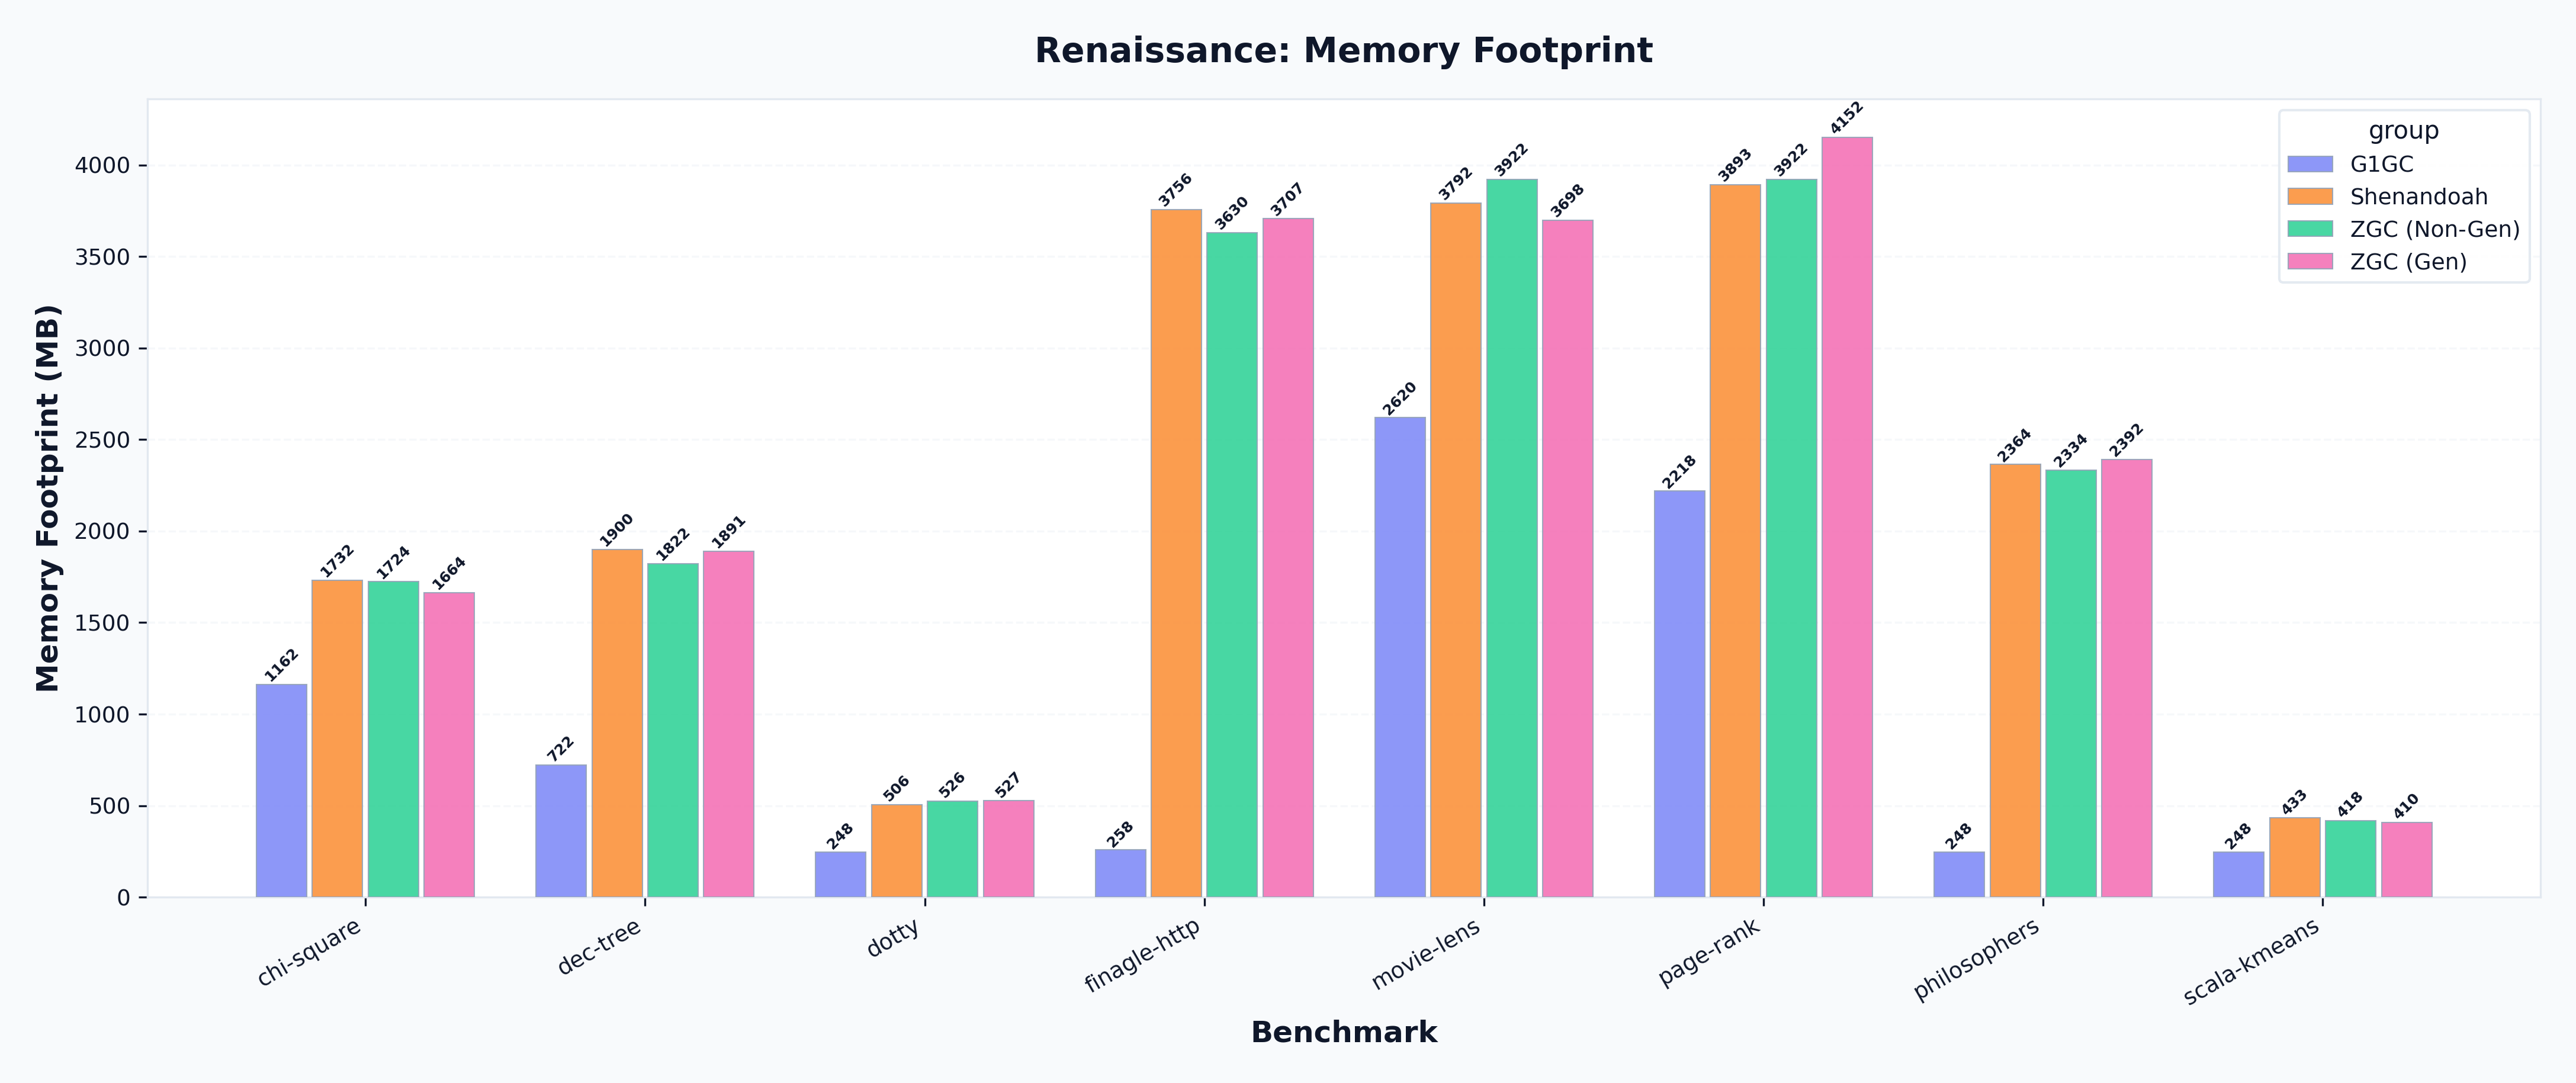
\includegraphics[width=\linewidth]{graphs/renaissance/renaissance_footprint.png}
\caption{Footprint}
\end{subfigure} &
\begin{subfigure}{0.45\textwidth}
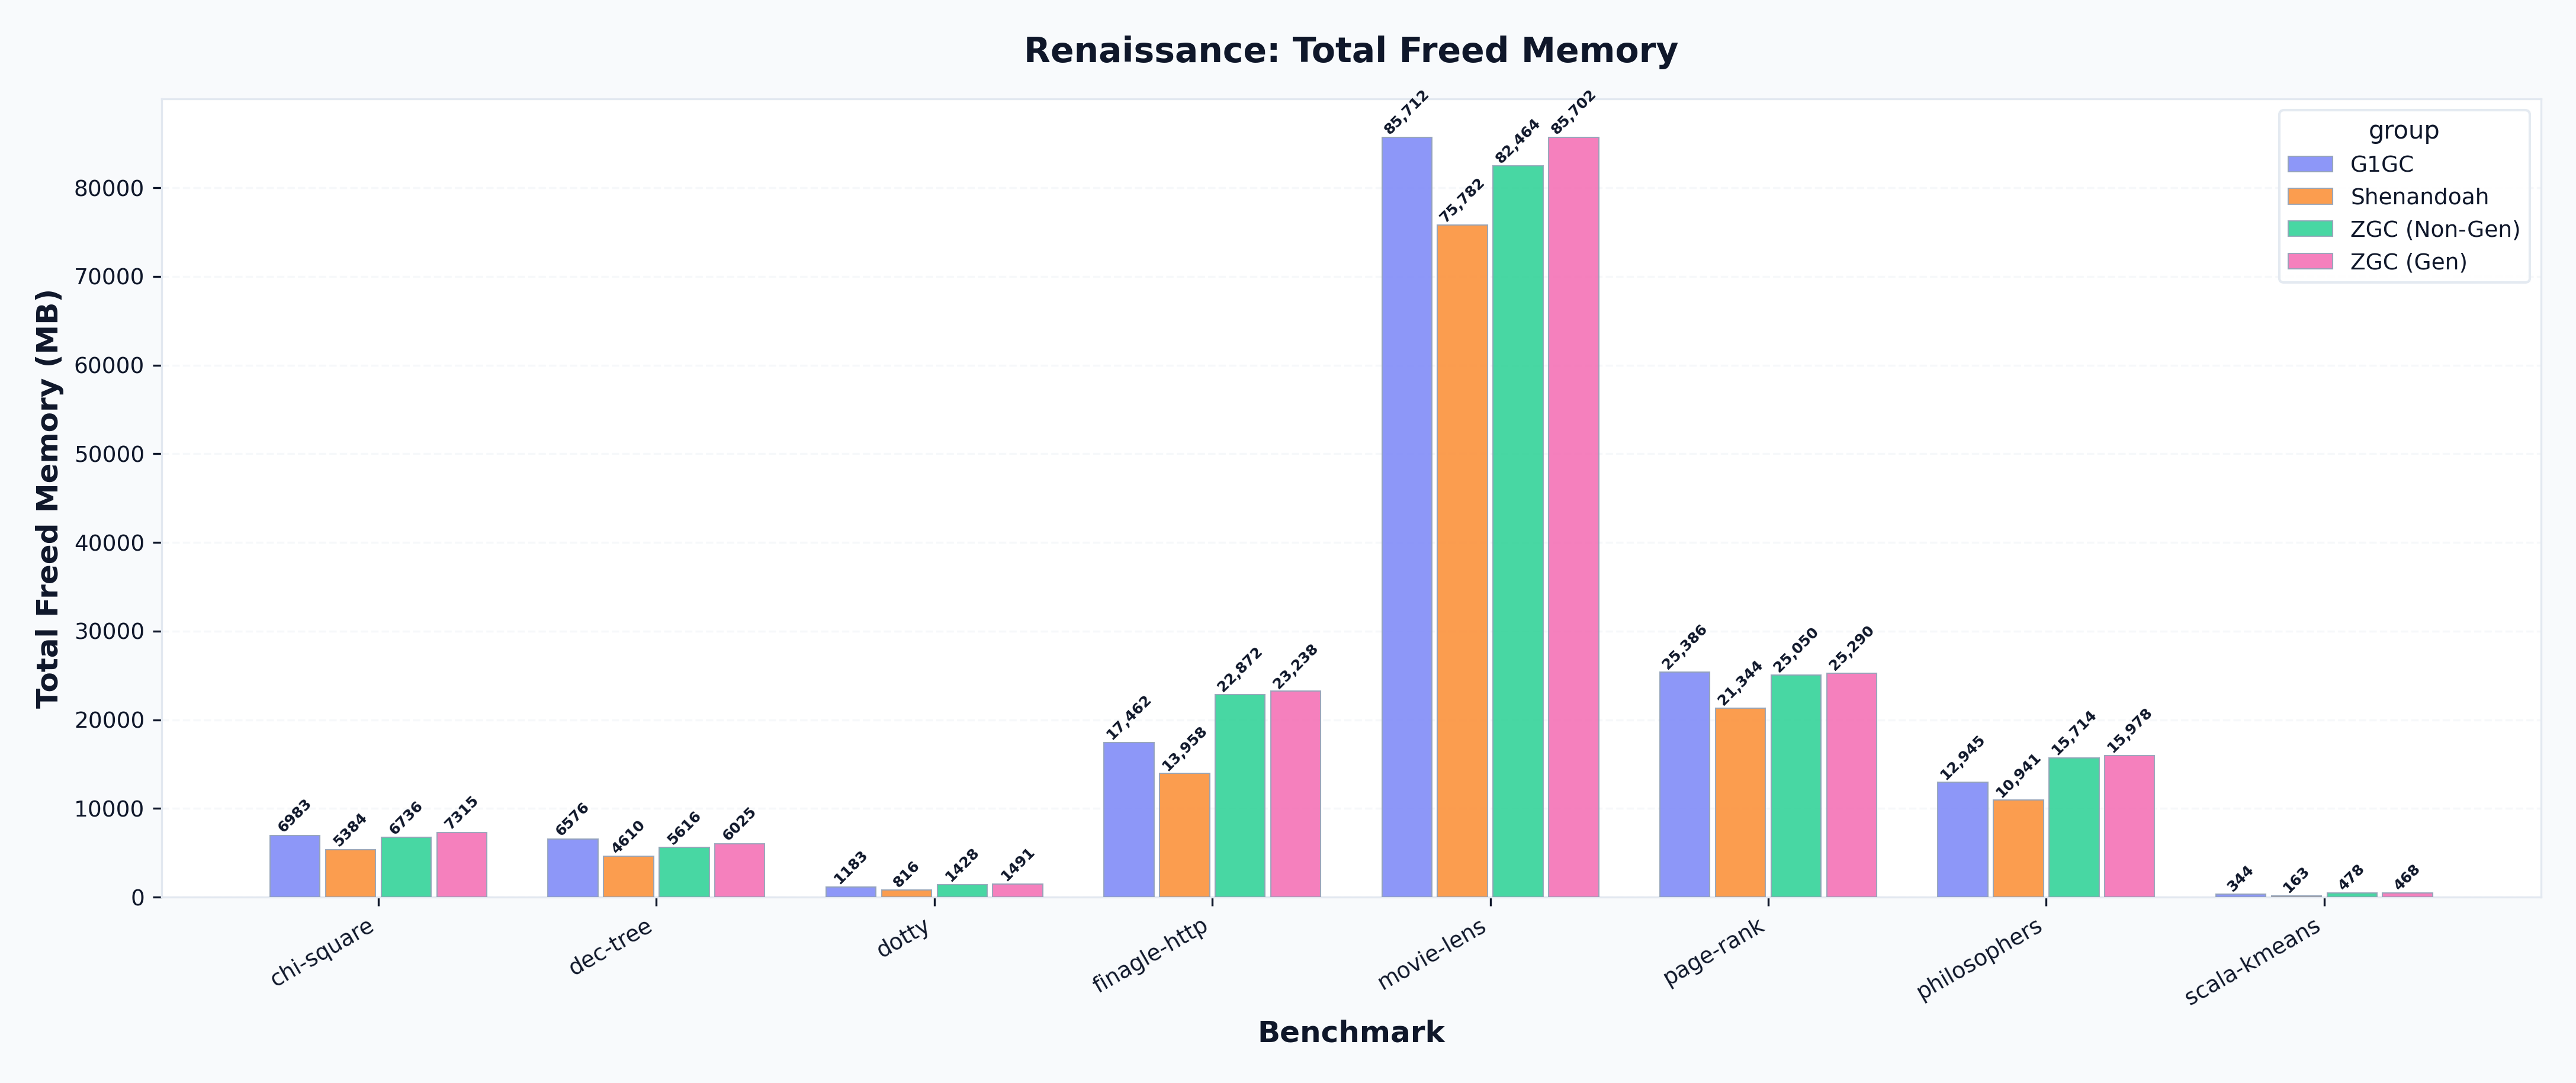
\includegraphics[width=\linewidth]{graphs/renaissance/renaissance_freedMemory.png}
\caption{Freed Memory}
\end{subfigure} \\

\begin{subfigure}{0.45\textwidth}
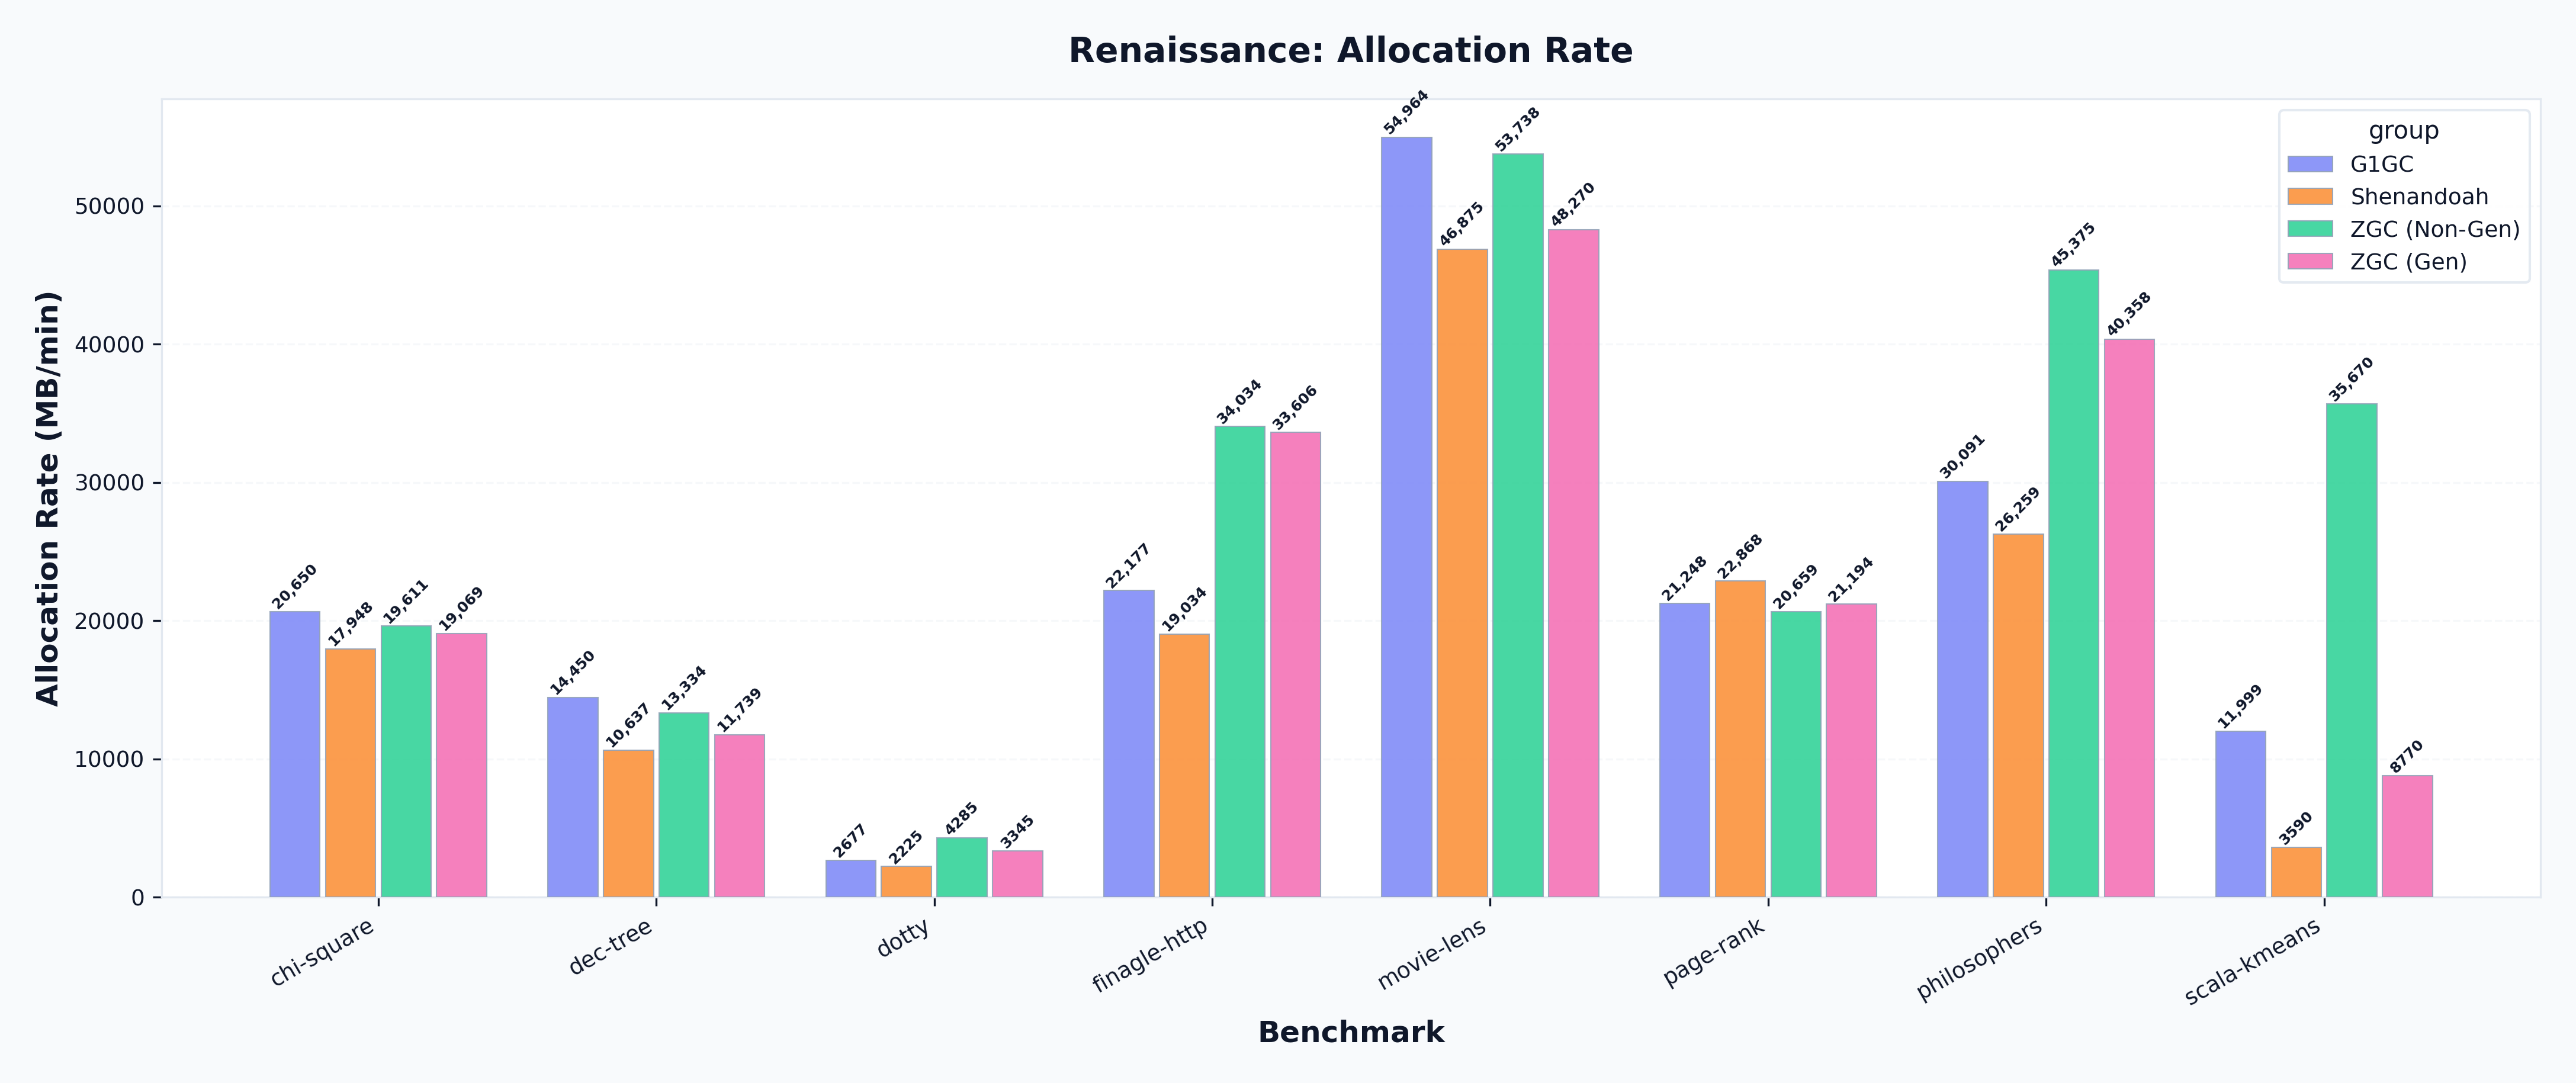
\includegraphics[width=\linewidth]{graphs/renaissance/renaissance_freedMemoryPerMin.png}
\caption{Freed Memory per Min}
\end{subfigure} &
\begin{subfigure}{0.45\textwidth}
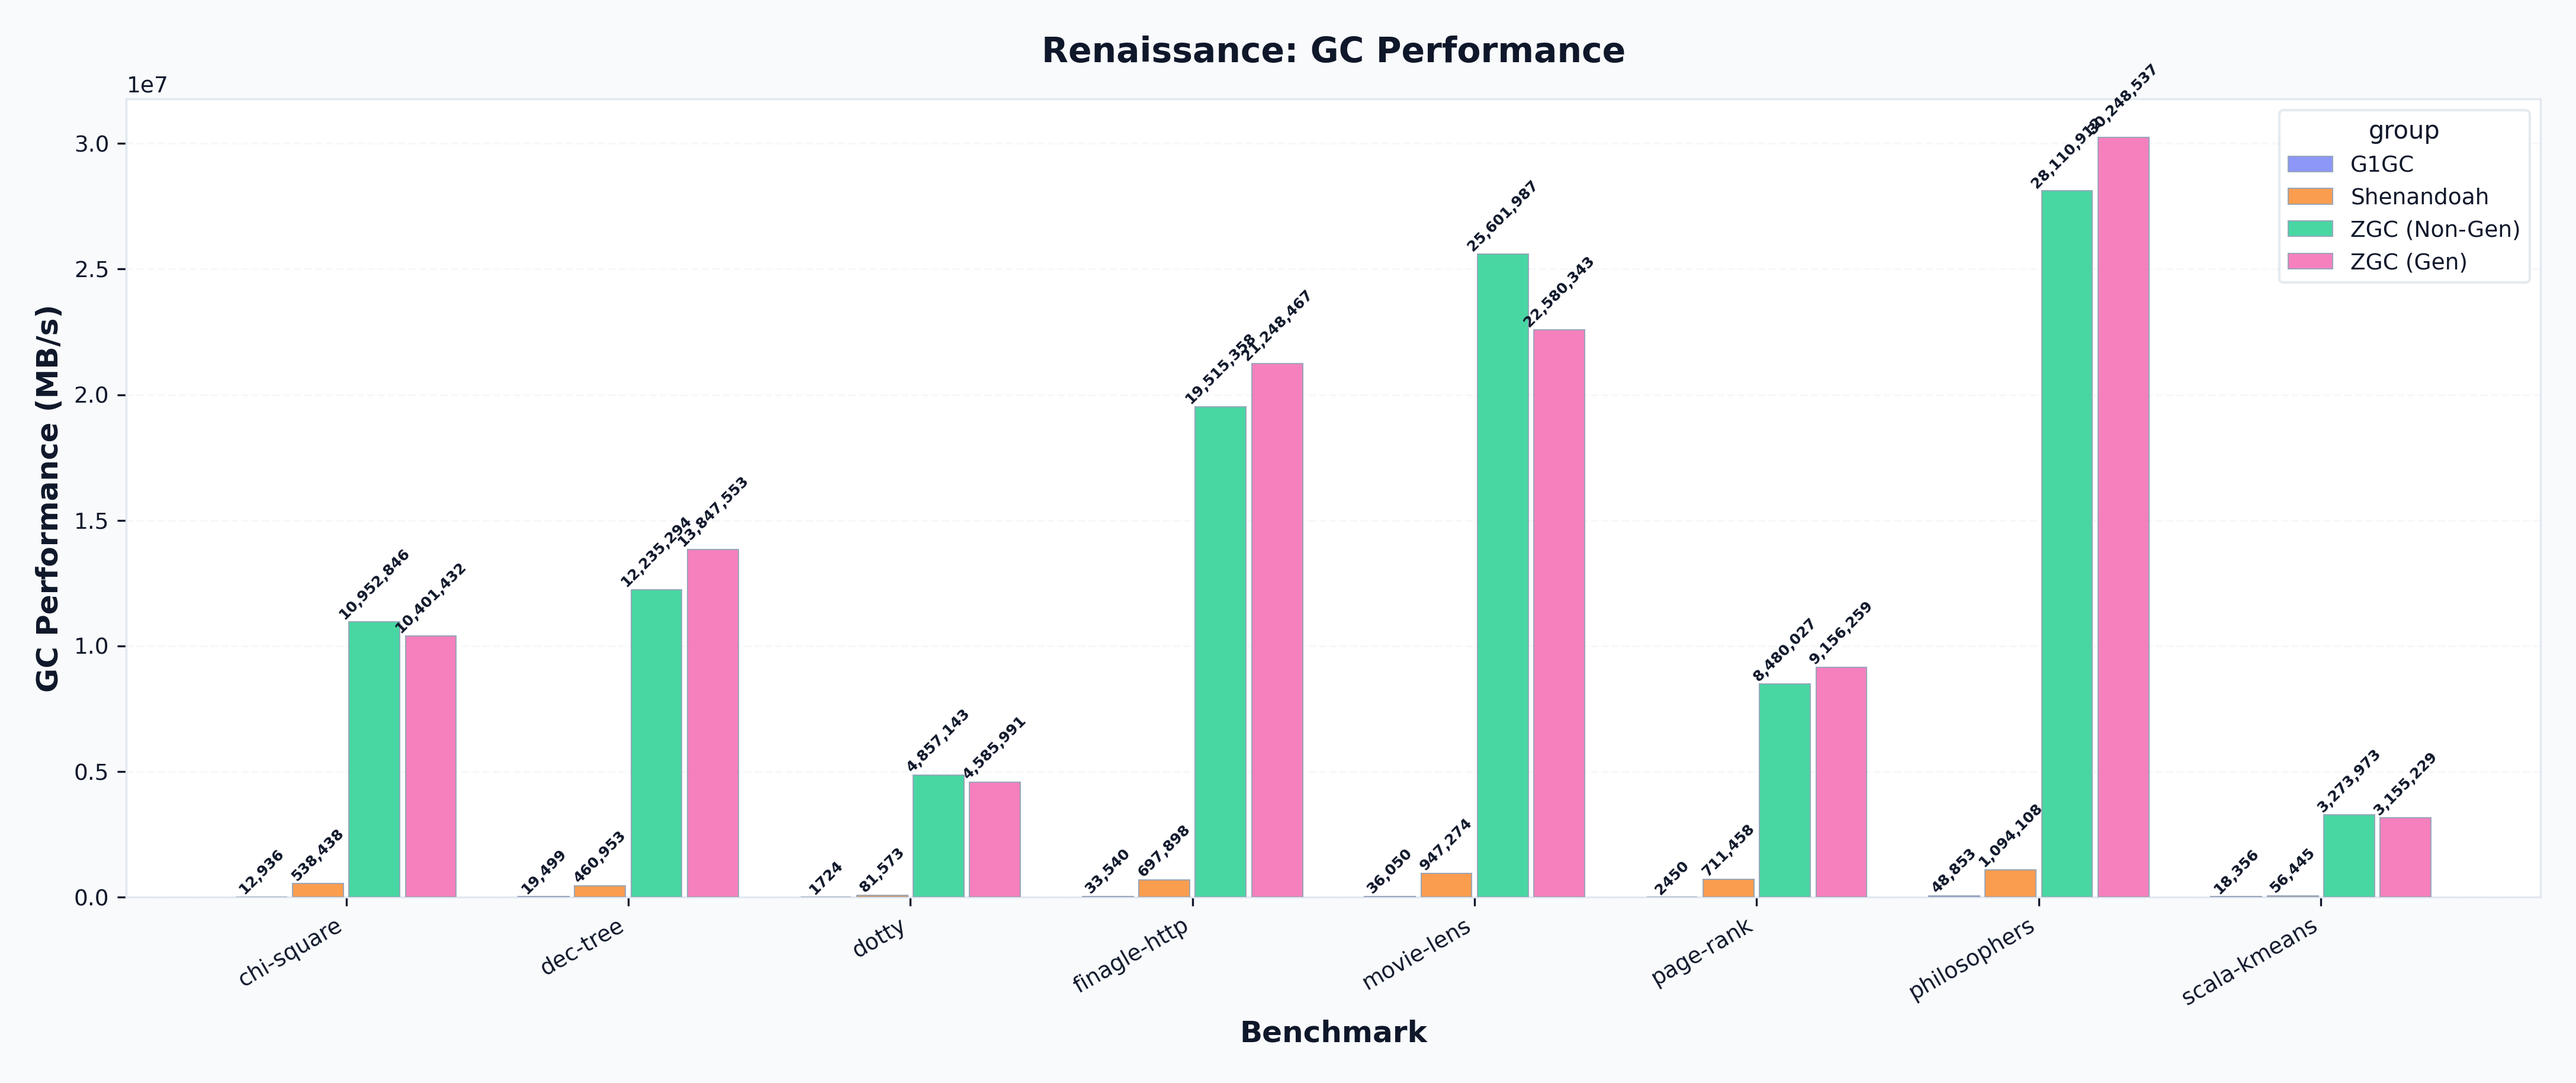
\includegraphics[width=\linewidth]{graphs/renaissance/renaissance_gcPerformance.png}
\caption{GC Performance}
\end{subfigure} \\

\begin{subfigure}{0.45\textwidth}
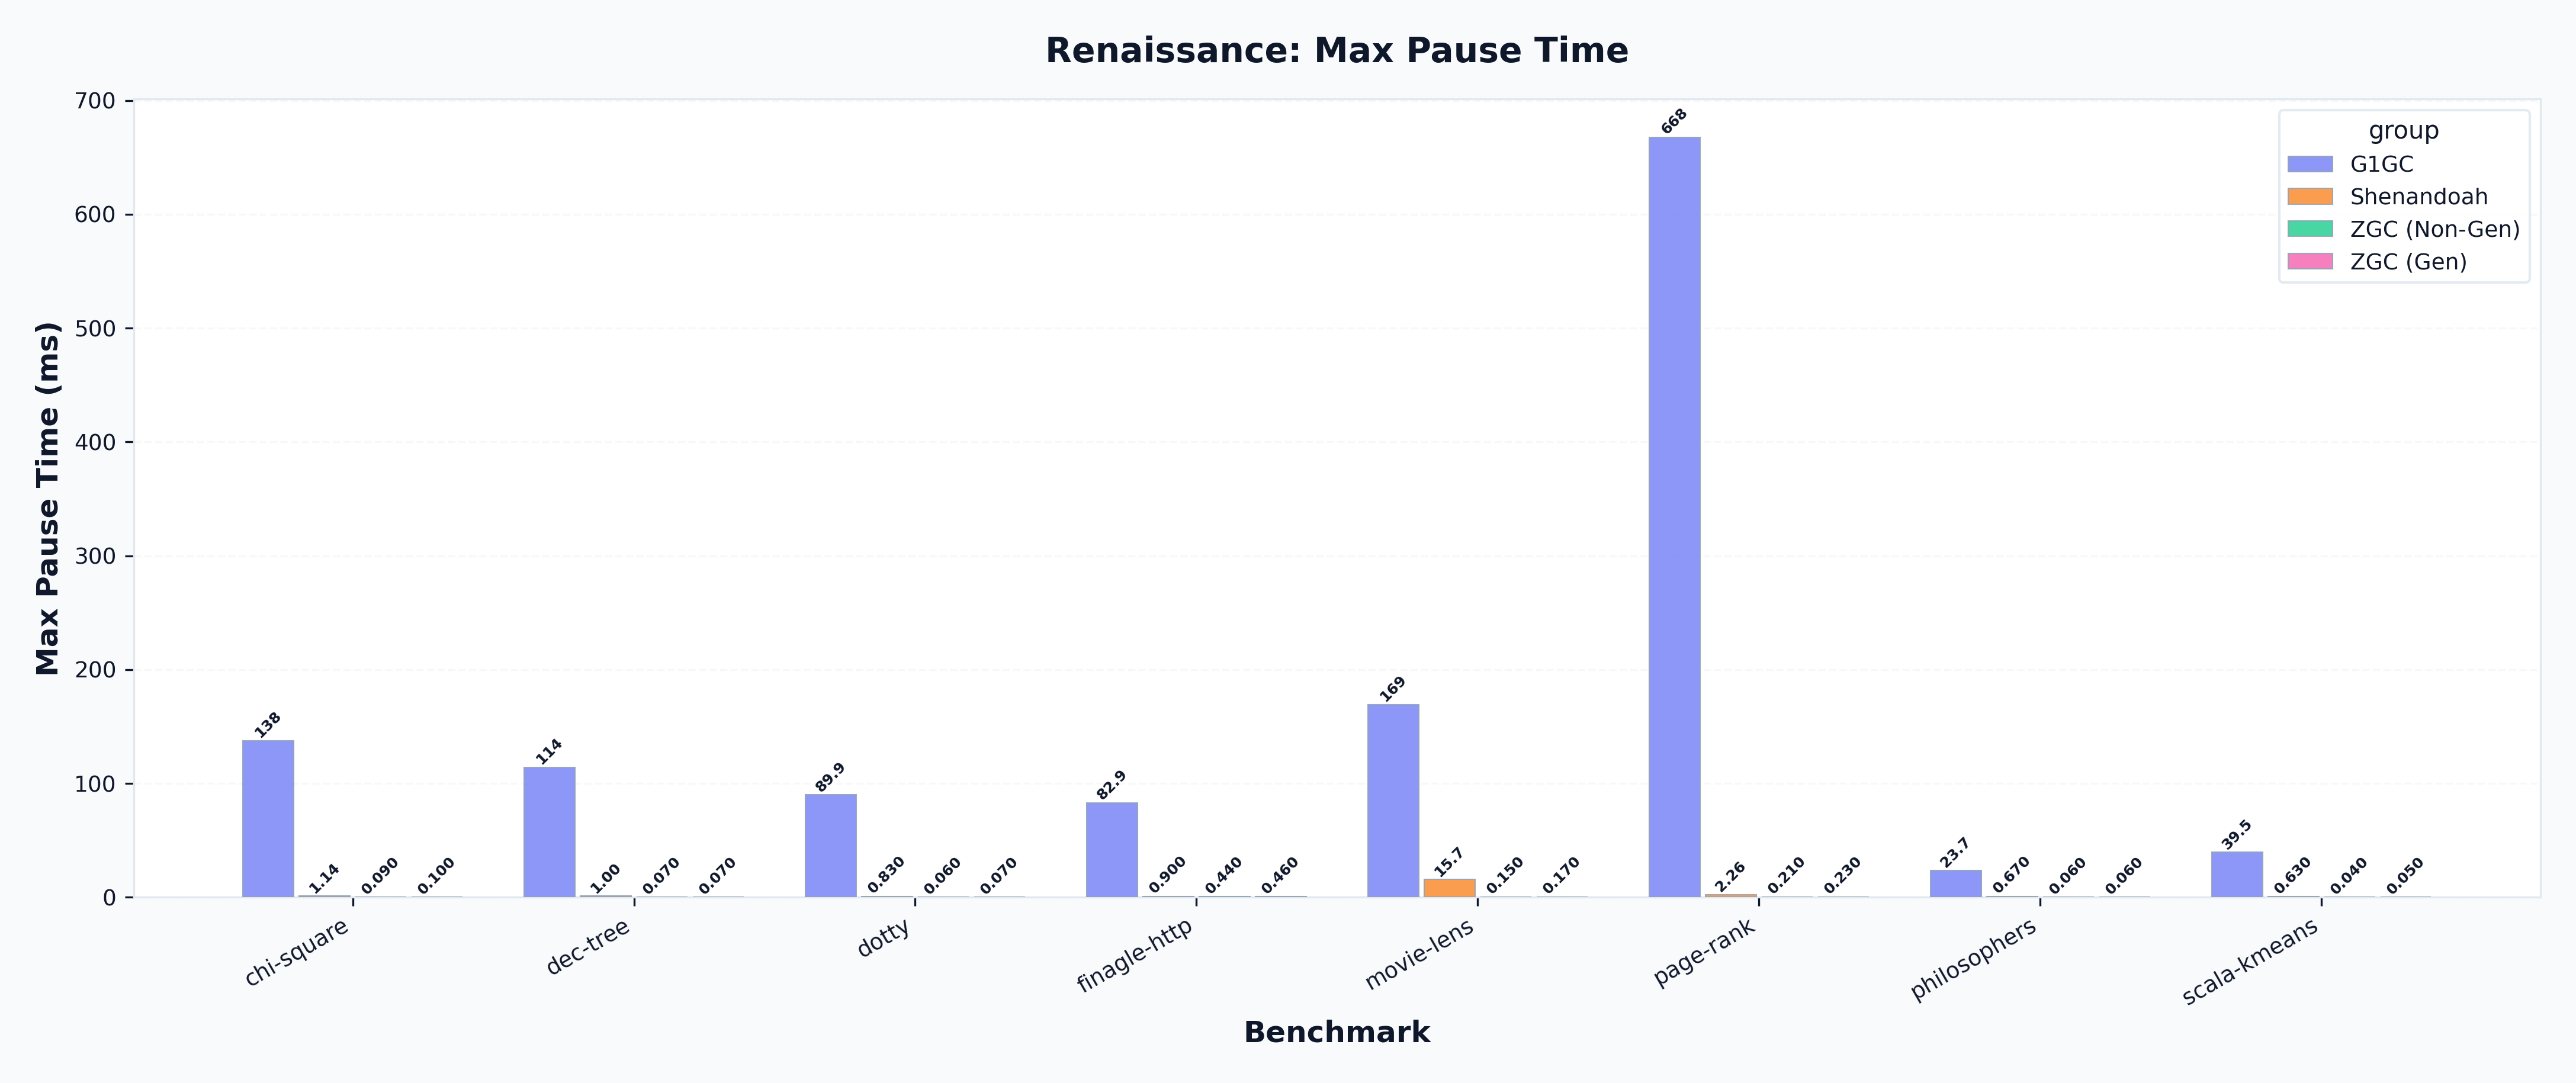
\includegraphics[width=\linewidth]{graphs/renaissance/renaissance_maxPause.png}
\caption{Max Pause}
\end{subfigure} &
\begin{subfigure}{0.45\textwidth}
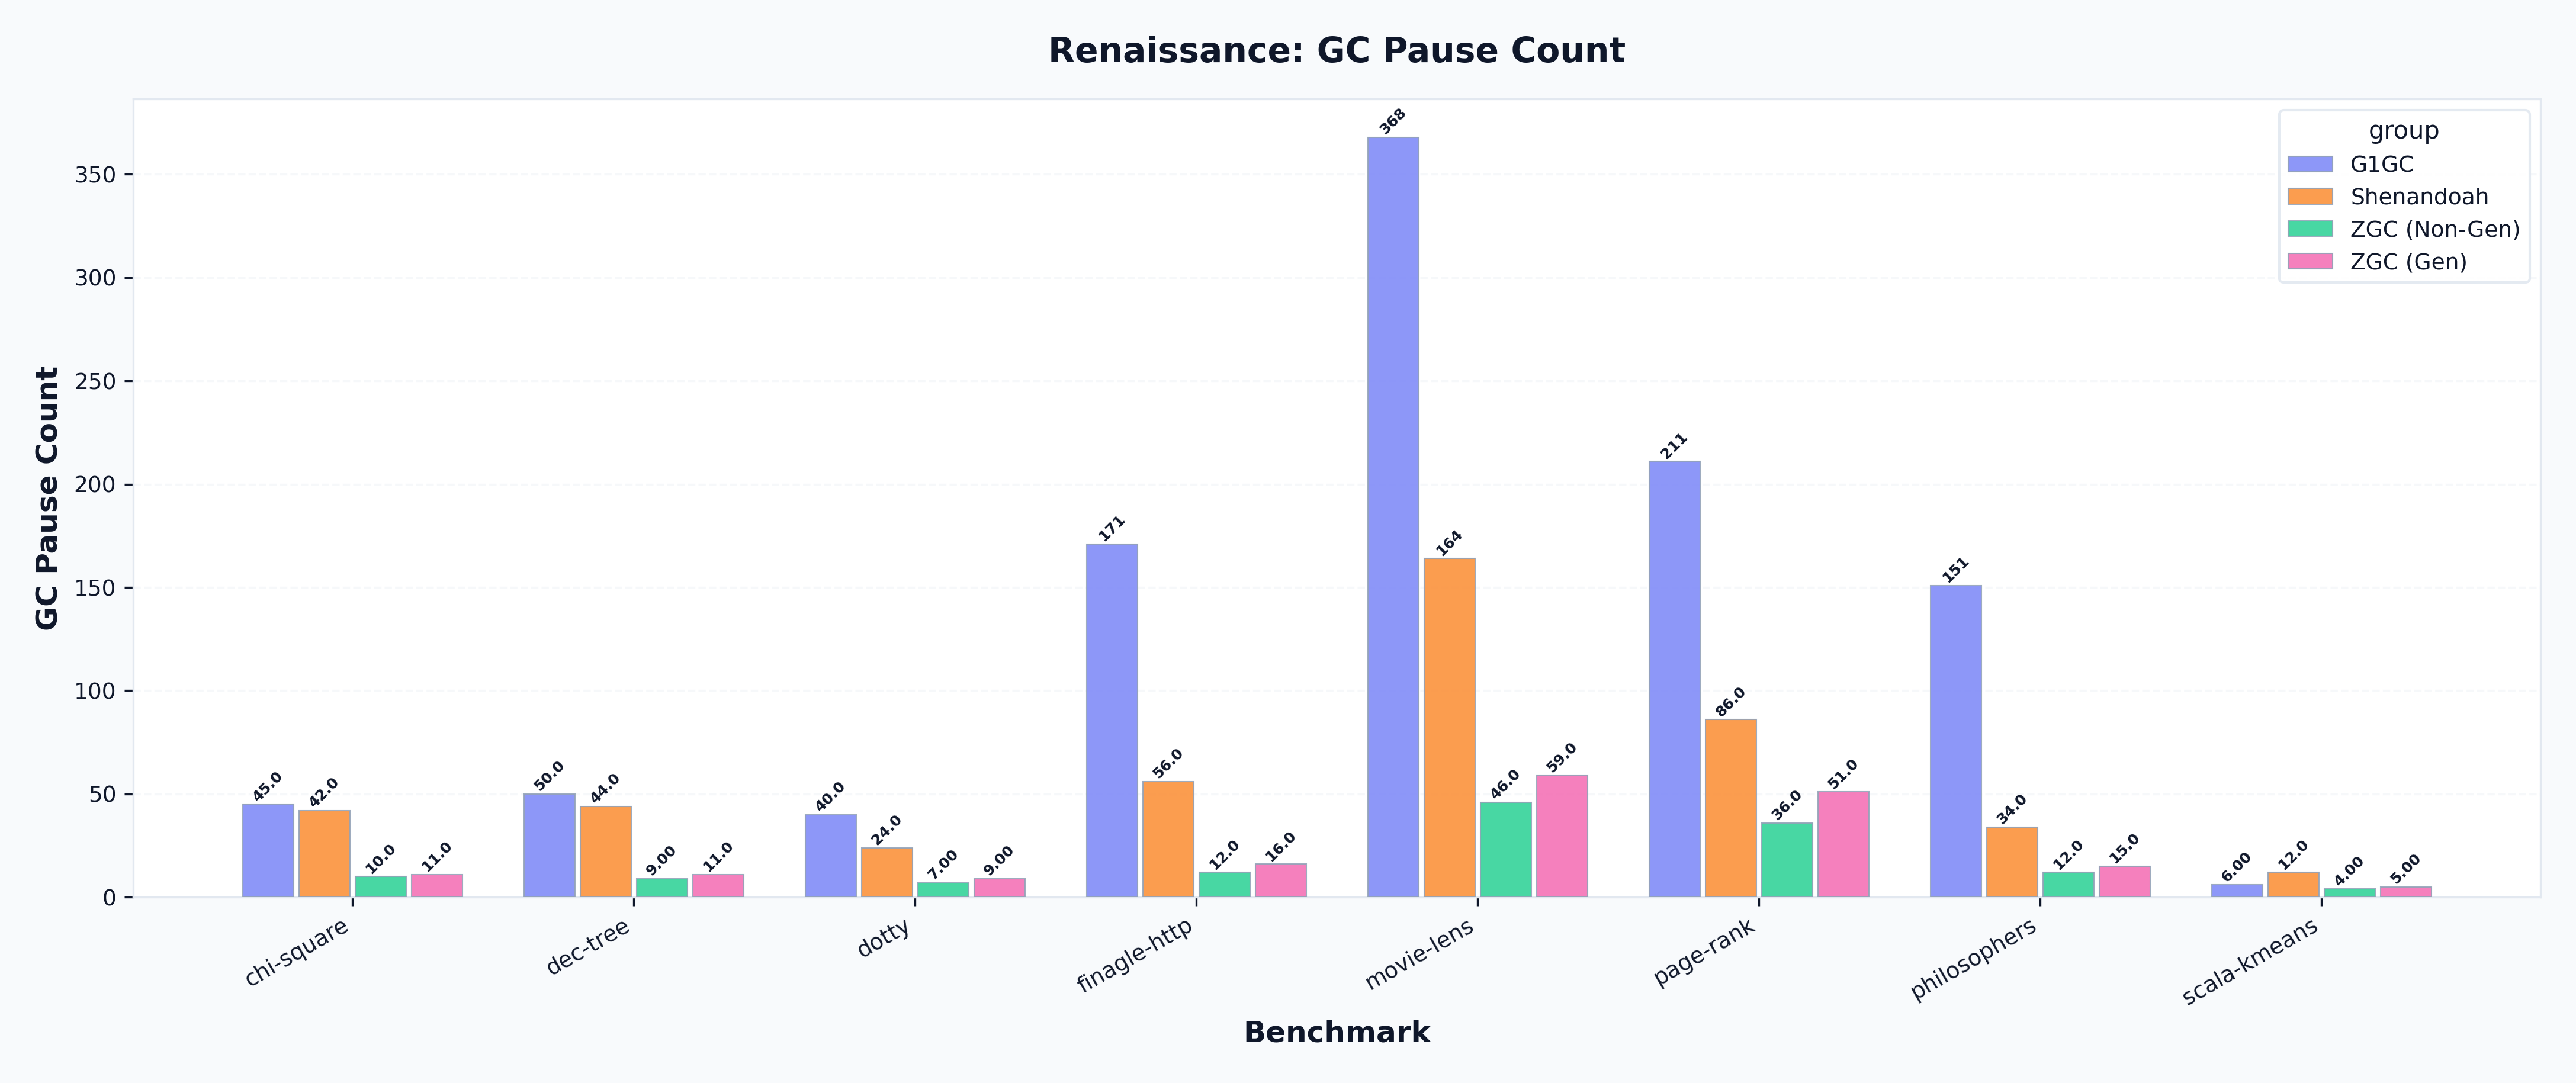
\includegraphics[width=\linewidth]{graphs/renaissance/renaissance_pauseCount.png}
\caption{Pause Count}
\end{subfigure} \\

\begin{subfigure}{0.45\textwidth}
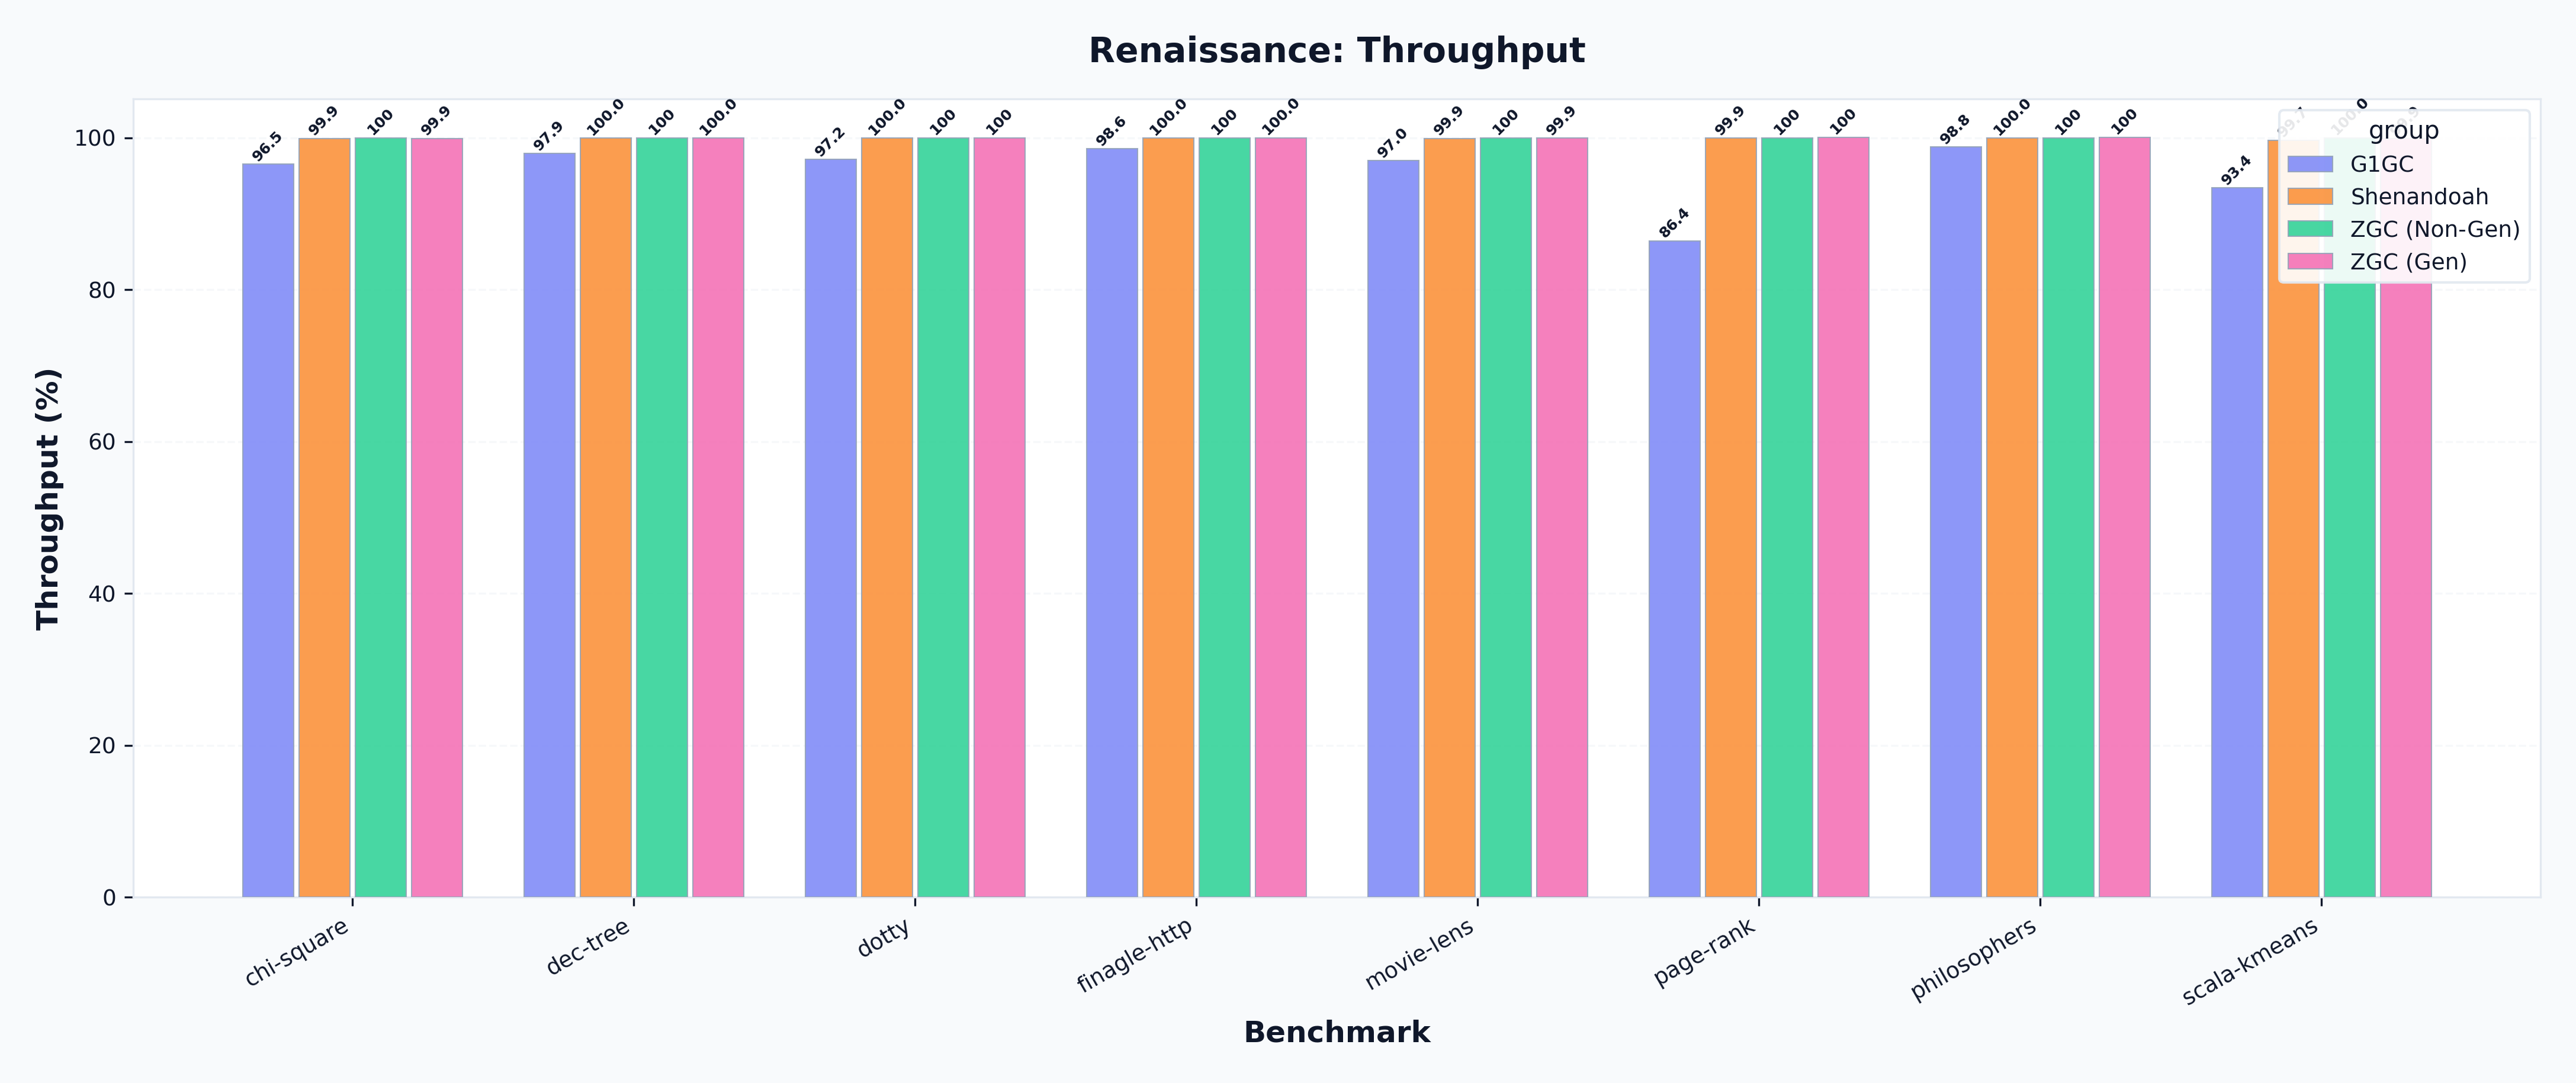
\includegraphics[width=\linewidth]{graphs/renaissance/renaissance_throughput.png}
\caption{Throughput}
\end{subfigure} &
\begin{subfigure}{0.45\textwidth}
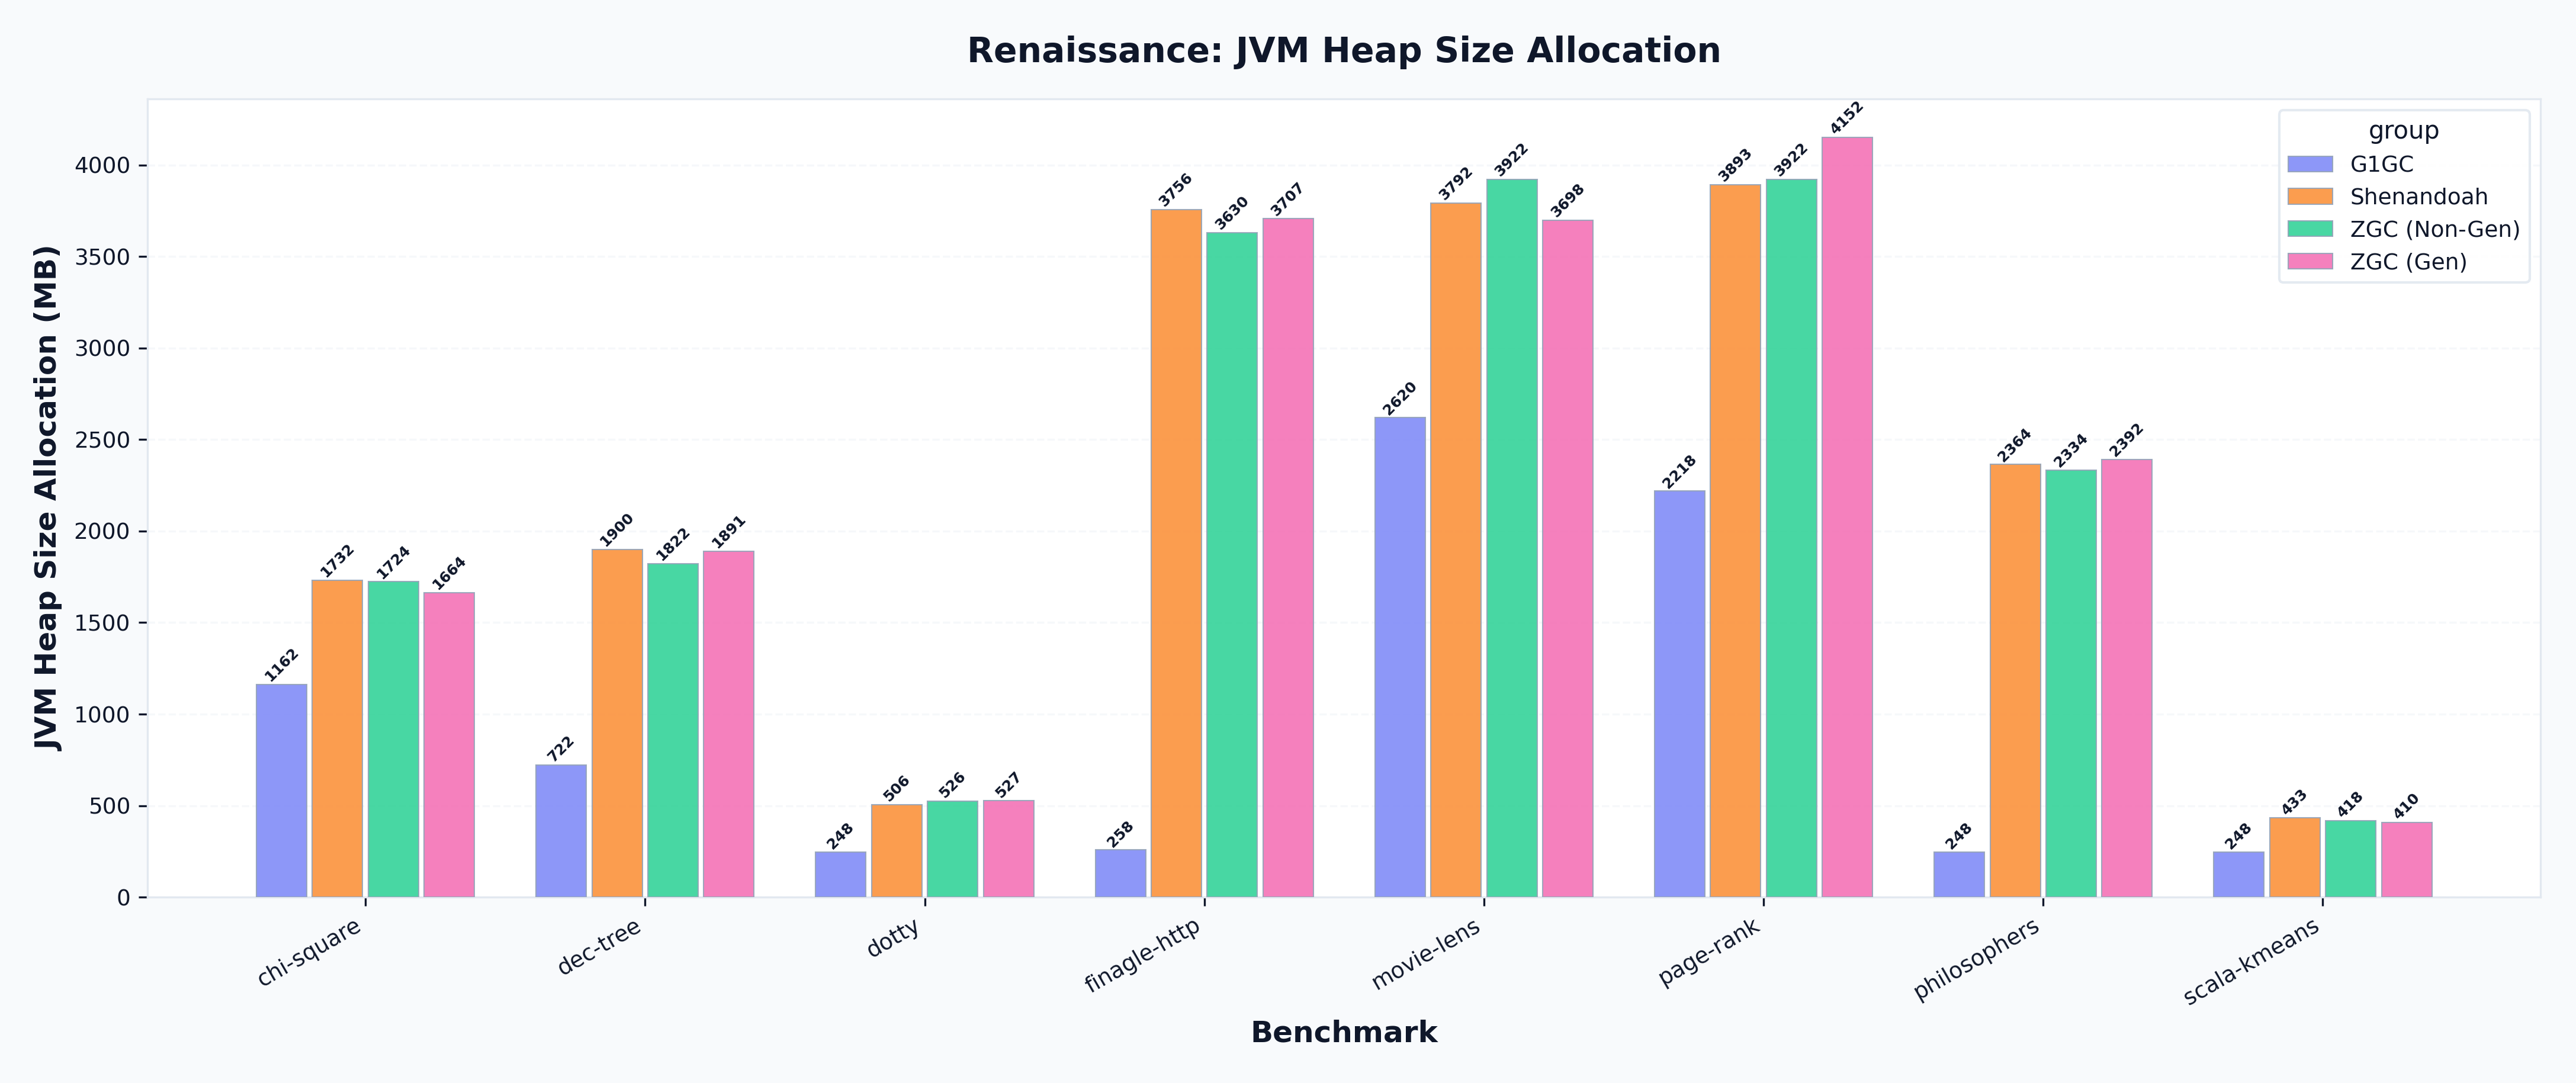
\includegraphics[width=\linewidth]{graphs/renaissance/renaissance_totalHeapAllocMax.png}
\caption{Total Heap Alloc Max}
\end{subfigure} \\

\begin{subfigure}{0.45\textwidth}
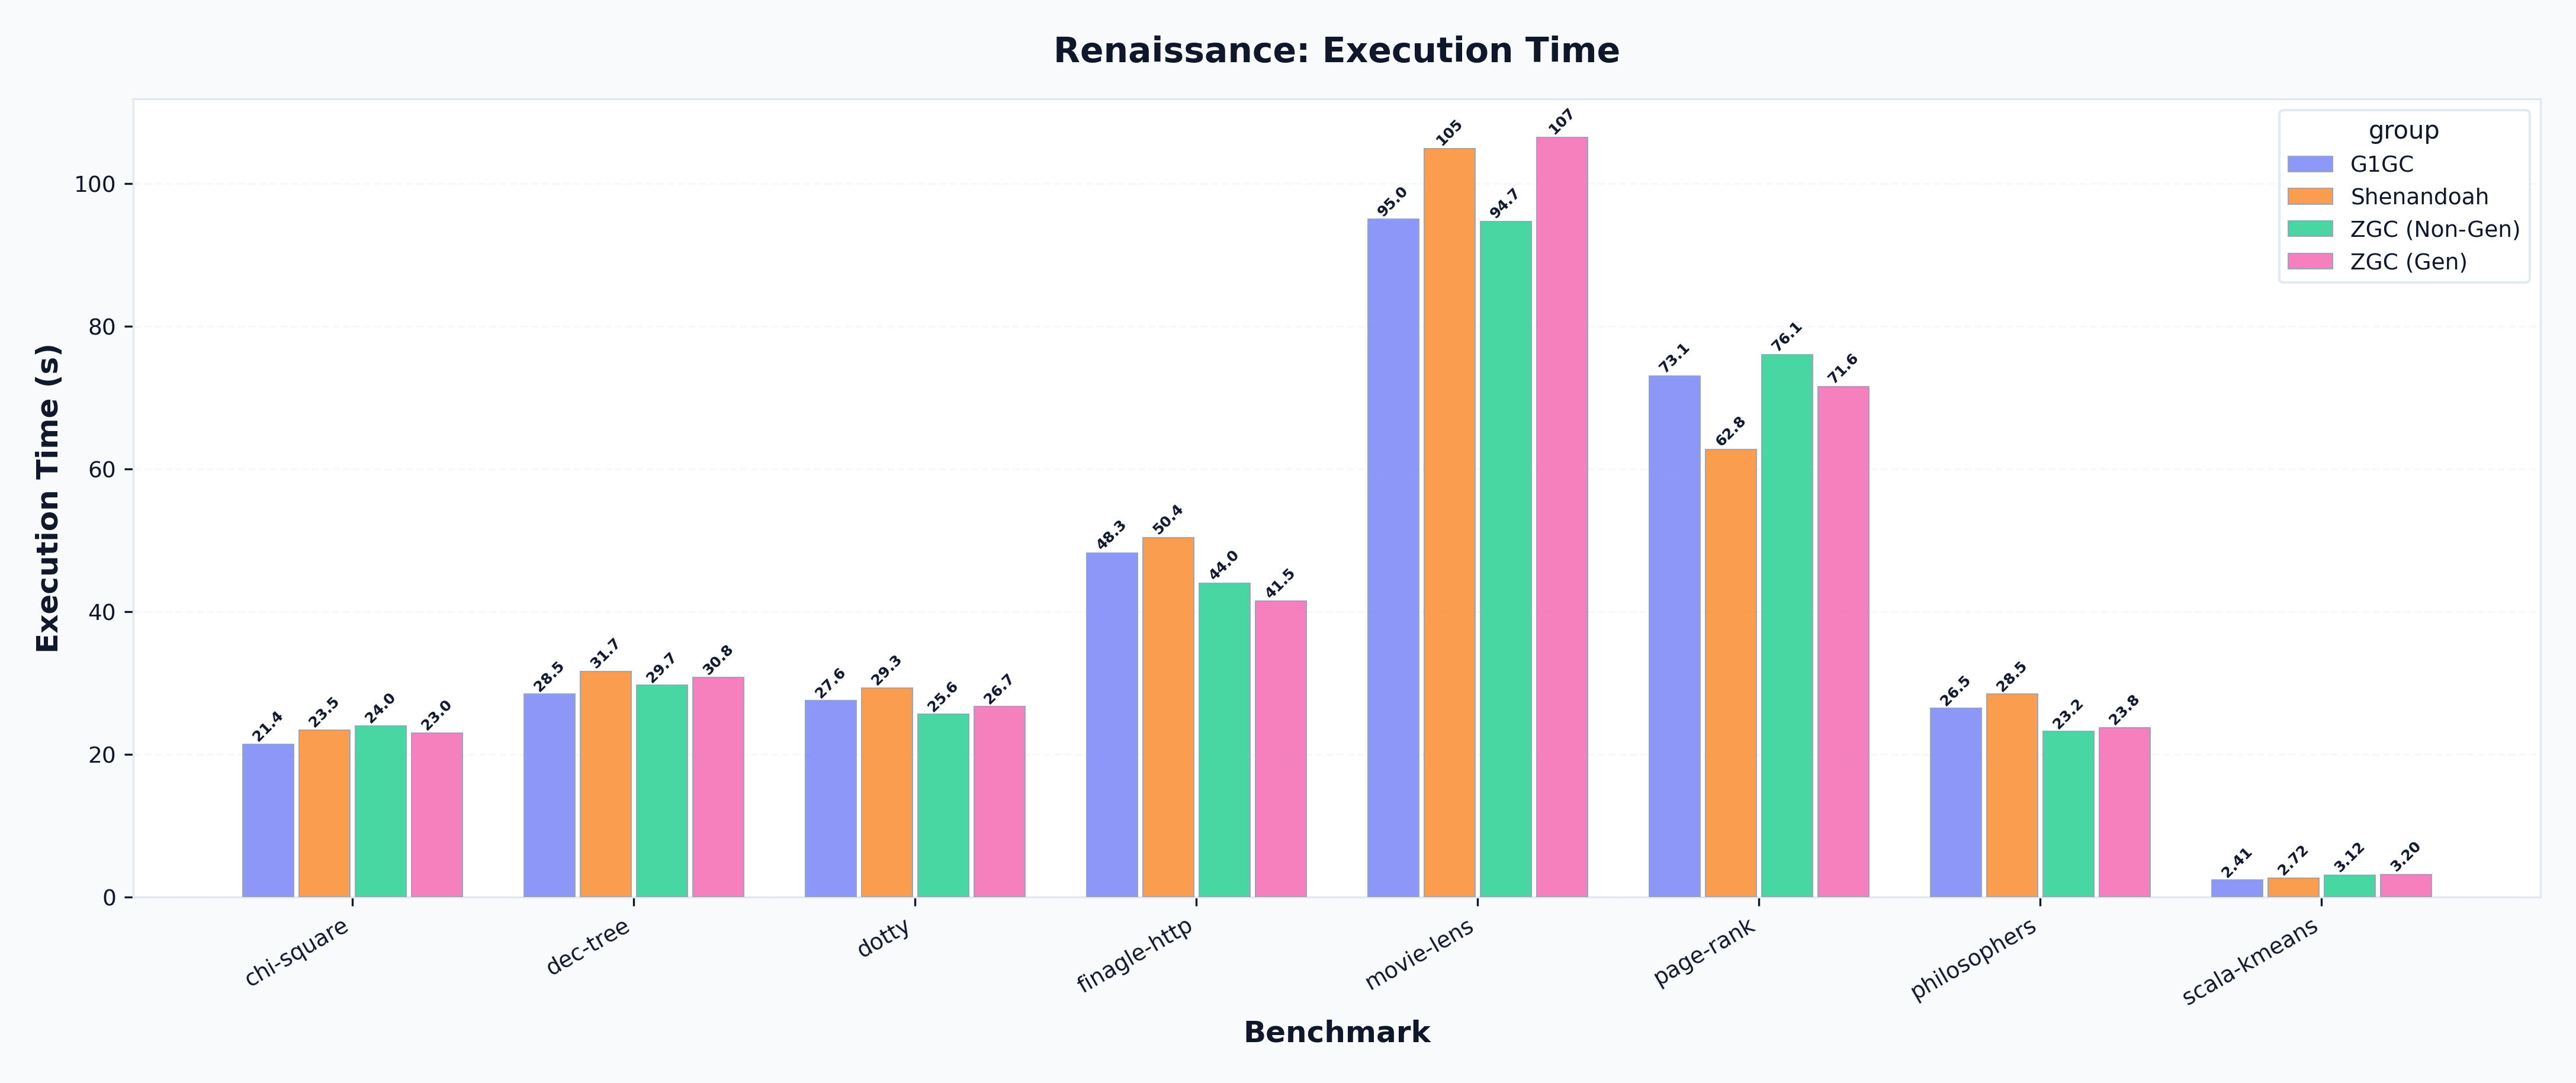
\includegraphics[width=\linewidth]{graphs/renaissance/renaissance_wallTimeSec.png}
\caption{Wall Time (sec)}
\end{subfigure} &
\begin{subfigure}{0.45\textwidth}
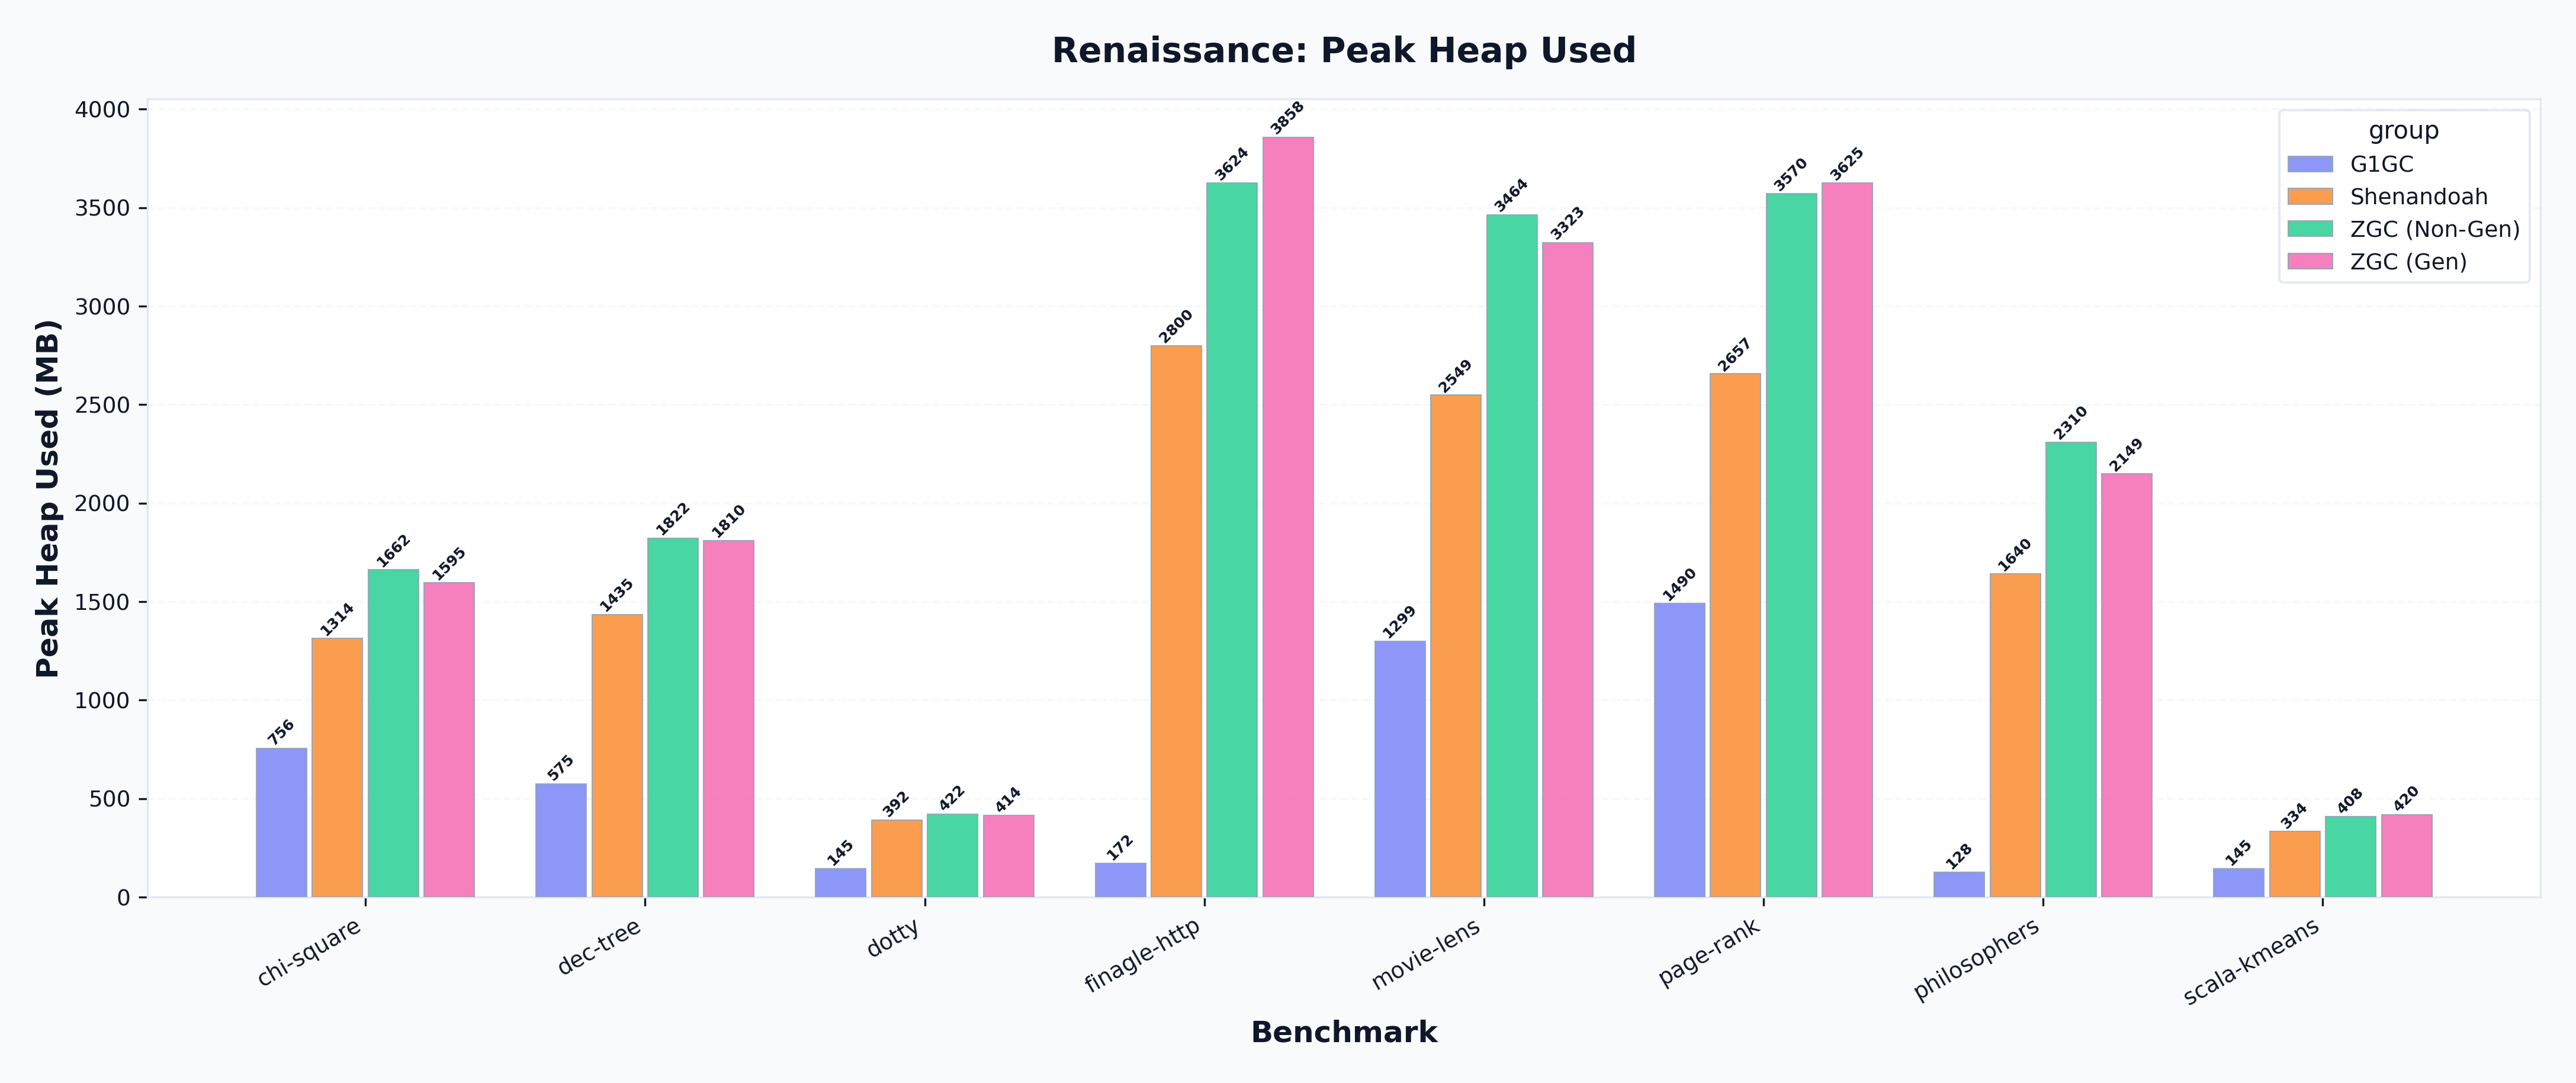
\includegraphics[width=\linewidth]{graphs/renaissance/renaissance_totalHeapUsedMax.png}
\caption{Total Heap Used Max}
\end{subfigure} \\

\end{tabular}

\caption{Renaissance Benchmark Results Across Different Metrics}
\label{fig:renaissance_all_6x2}
\end{figure}


\subsubsection{Generational and Non-Generational ZGC Comparison}
We also conducted a focused comparison between Generational and Non-Generational ZGC architectures to evaluate the impact of separating objects by age. As illustrated in Figure \ref{fig:dacapo_zgc_comparison} and Figure \ref{fig:renaissance_zgc_comparison}, Generational ZGC consistently minimizes accumulated pause times—keeping them resolutely below the 1ms threshold—while boosting the rate of freed memory per minute by over 25\%. This generational approach effectively mitigates allocation stalls, yielding nearly a 10-12\% higher overall GC performance score compared to its predecessor. These numbers prove it highly effective in handling short-lived objects typical in modern JVM workloads with high allocation rates.

\begin{figure}[h]
\centering

\begin{tabular}{cc}

\begin{subfigure}{0.45\textwidth}
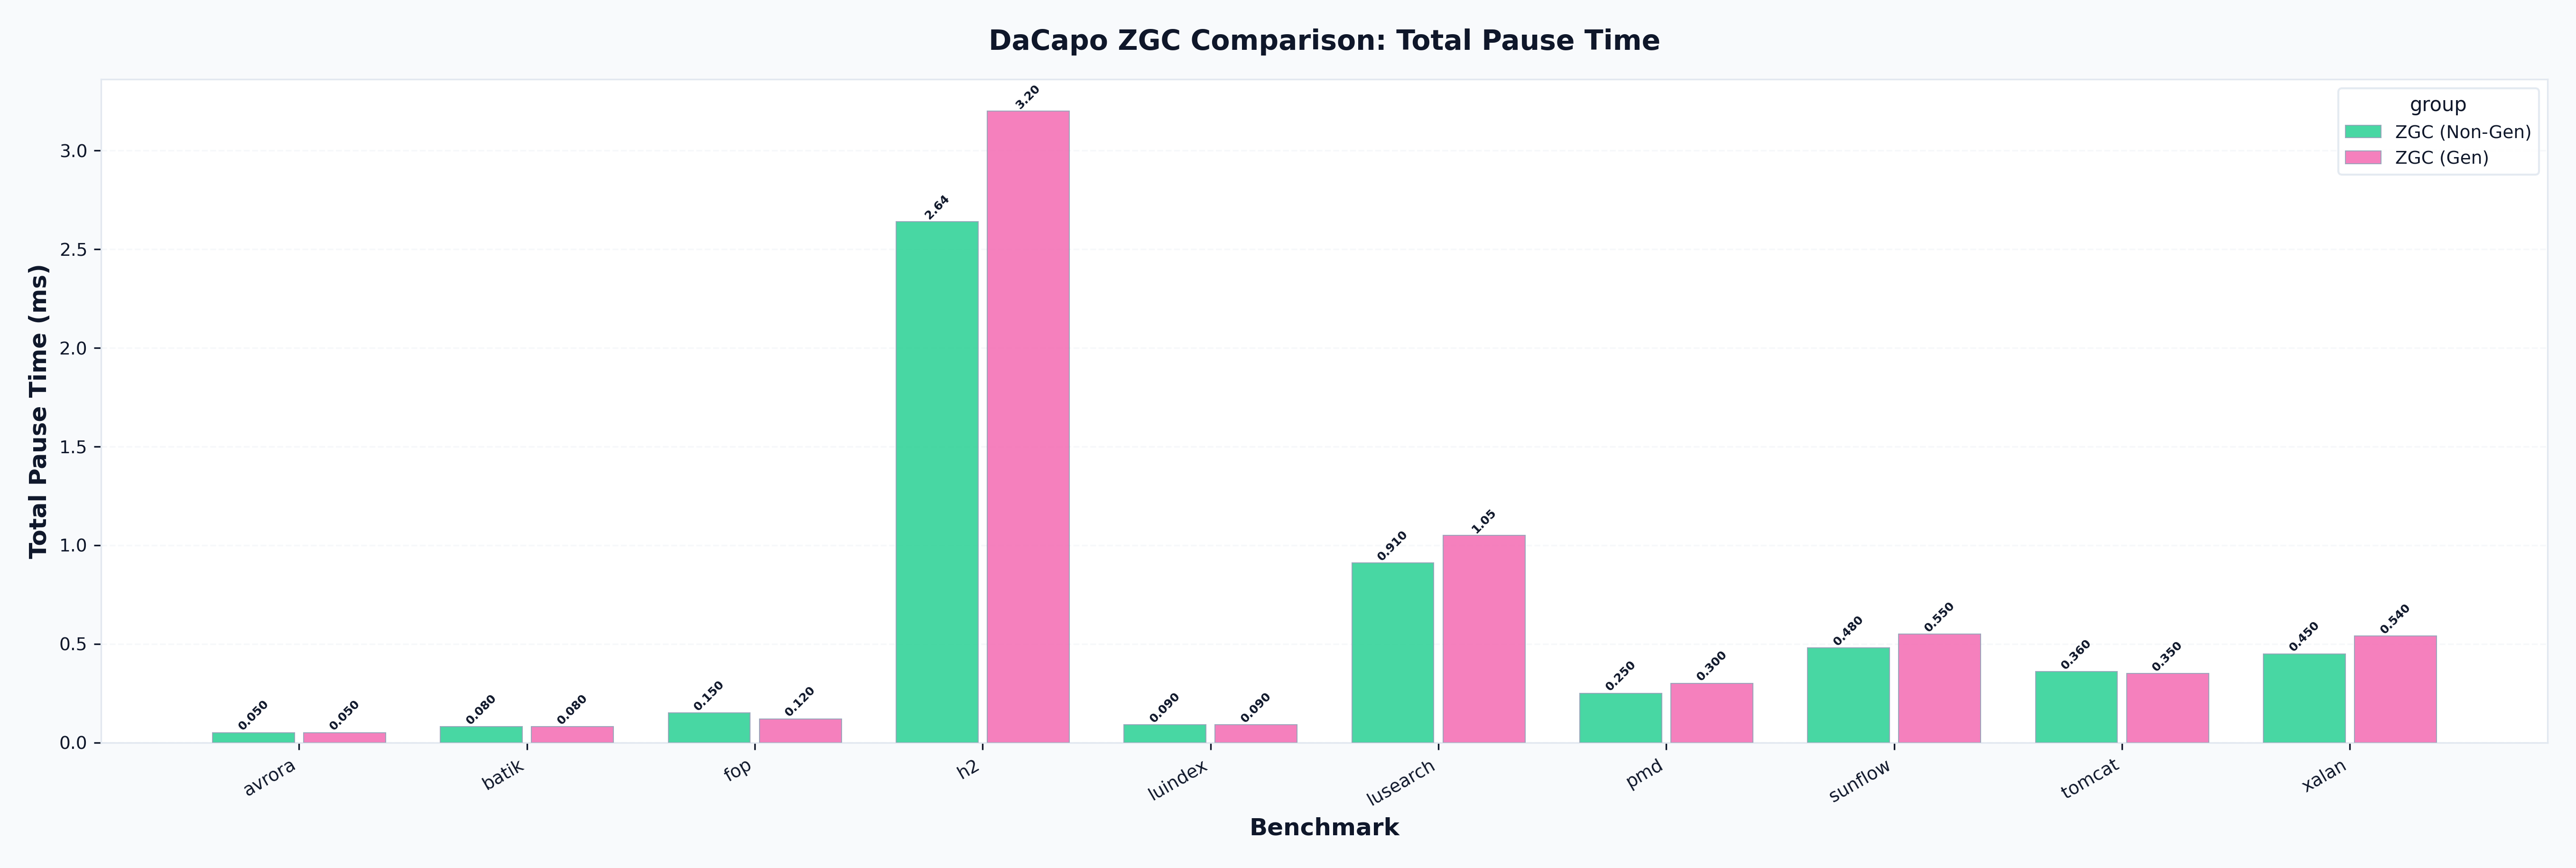
\includegraphics[width=\linewidth]{graphs/dacapo/zgc_comparison/dacapo_zgc_comparison_accumPause_zgc.png}
\caption{Accumulated Pause}
\end{subfigure} &
\begin{subfigure}{0.45\textwidth}
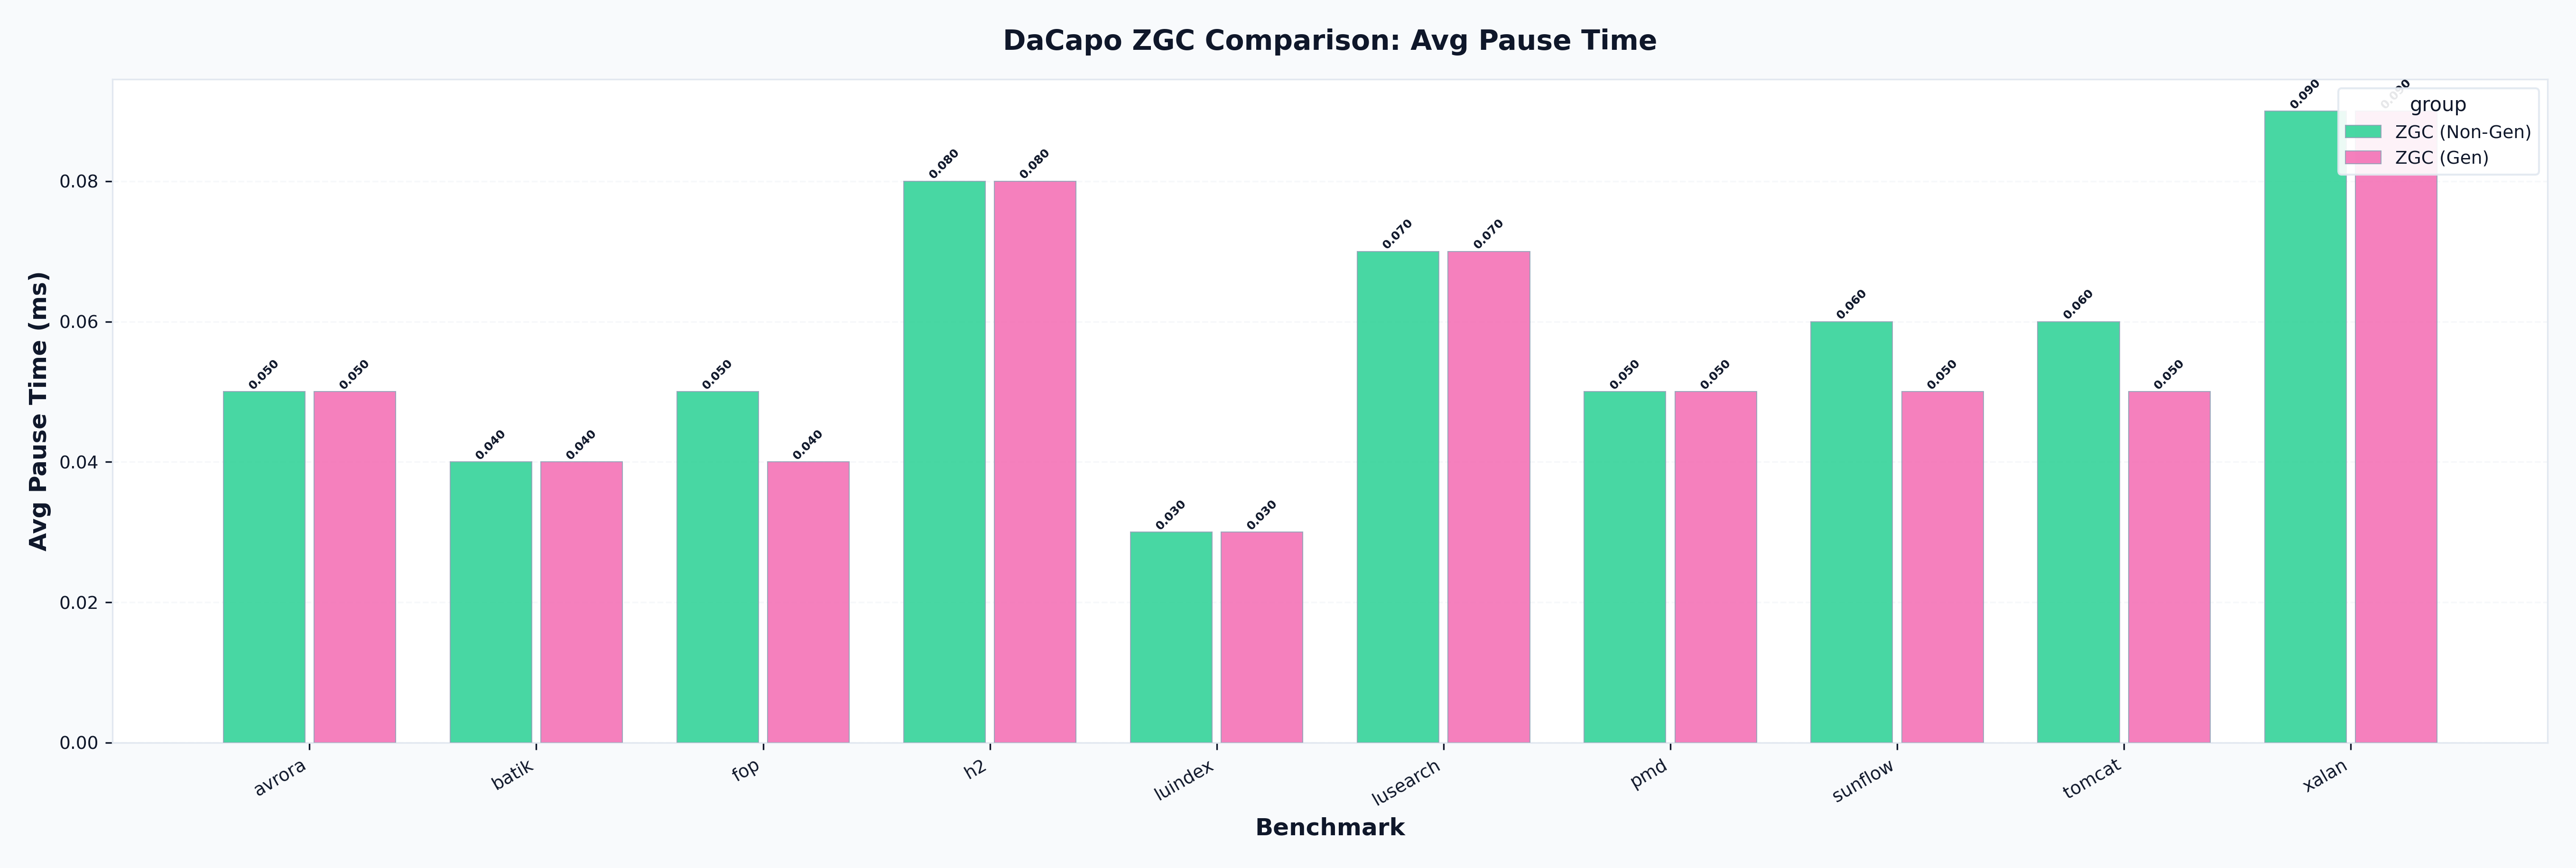
\includegraphics[width=\linewidth]{graphs/dacapo/zgc_comparison/dacapo_zgc_comparison_avgPause_zgc.png}
\caption{Average Pause}
\end{subfigure} \\

\begin{subfigure}{0.45\textwidth}
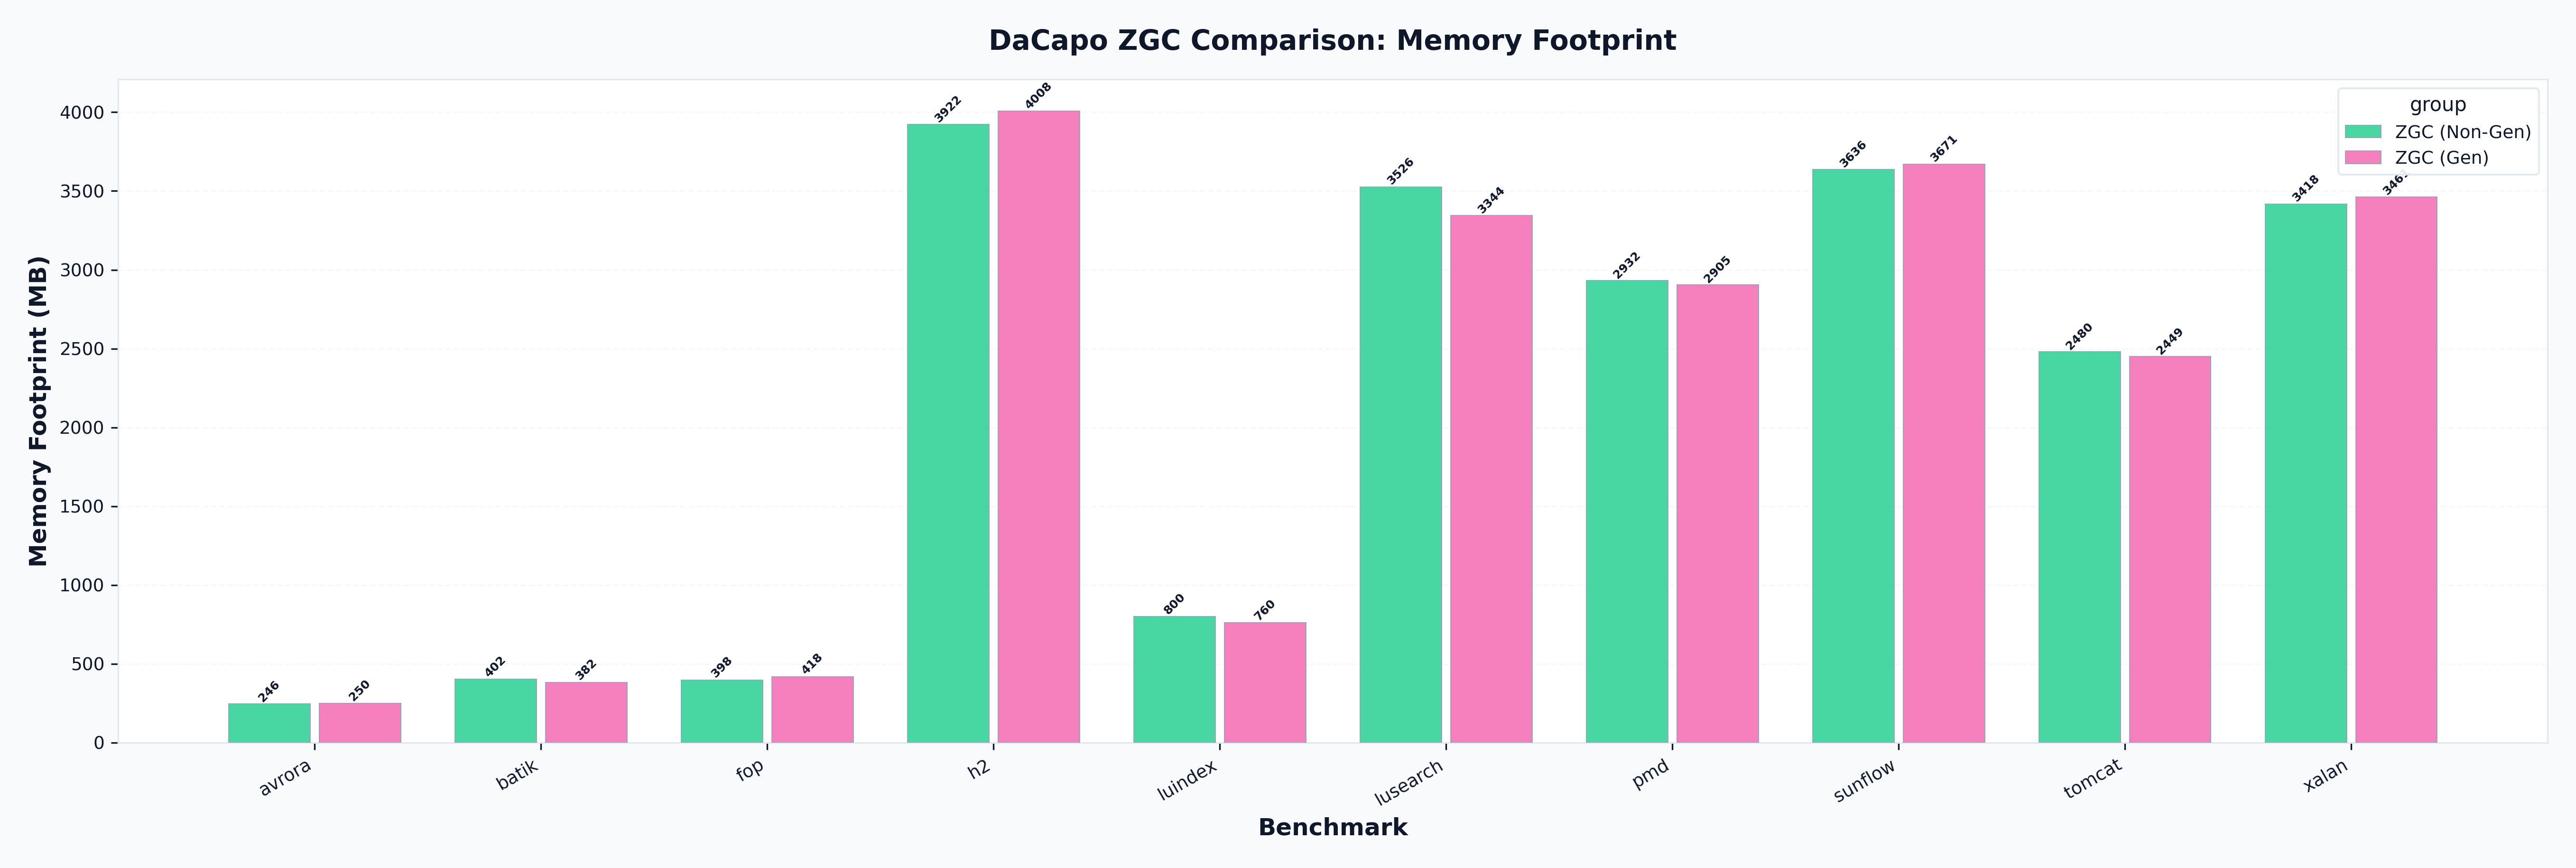
\includegraphics[width=\linewidth]{graphs/dacapo/zgc_comparison/dacapo_zgc_comparison_footprint_zgc.png}
\caption{Footprint}
\end{subfigure} &
\begin{subfigure}{0.45\textwidth}
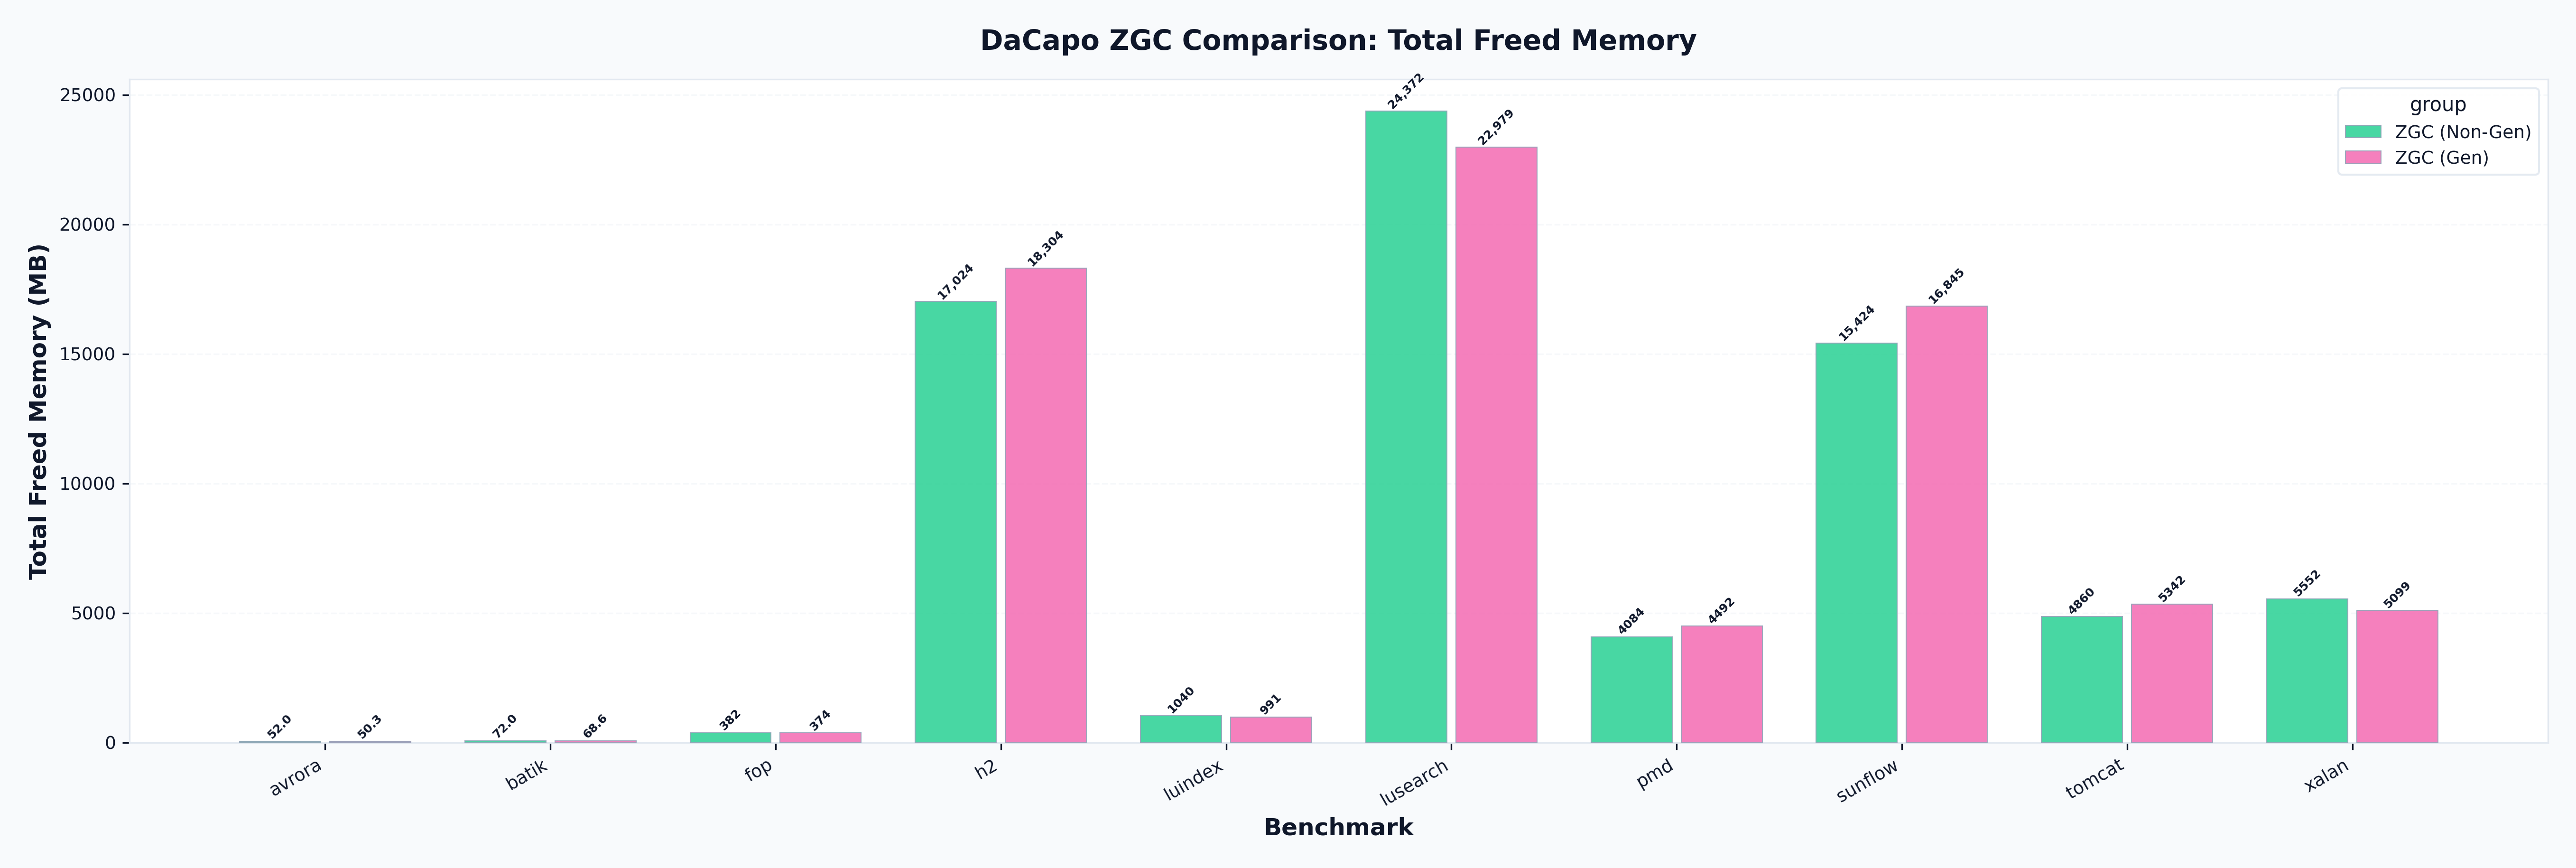
\includegraphics[width=\linewidth]{graphs/dacapo/zgc_comparison/dacapo_zgc_comparison_freedMemory_zgc.png}
\caption{Freed Memory}
\end{subfigure} \\

\begin{subfigure}{0.45\textwidth}
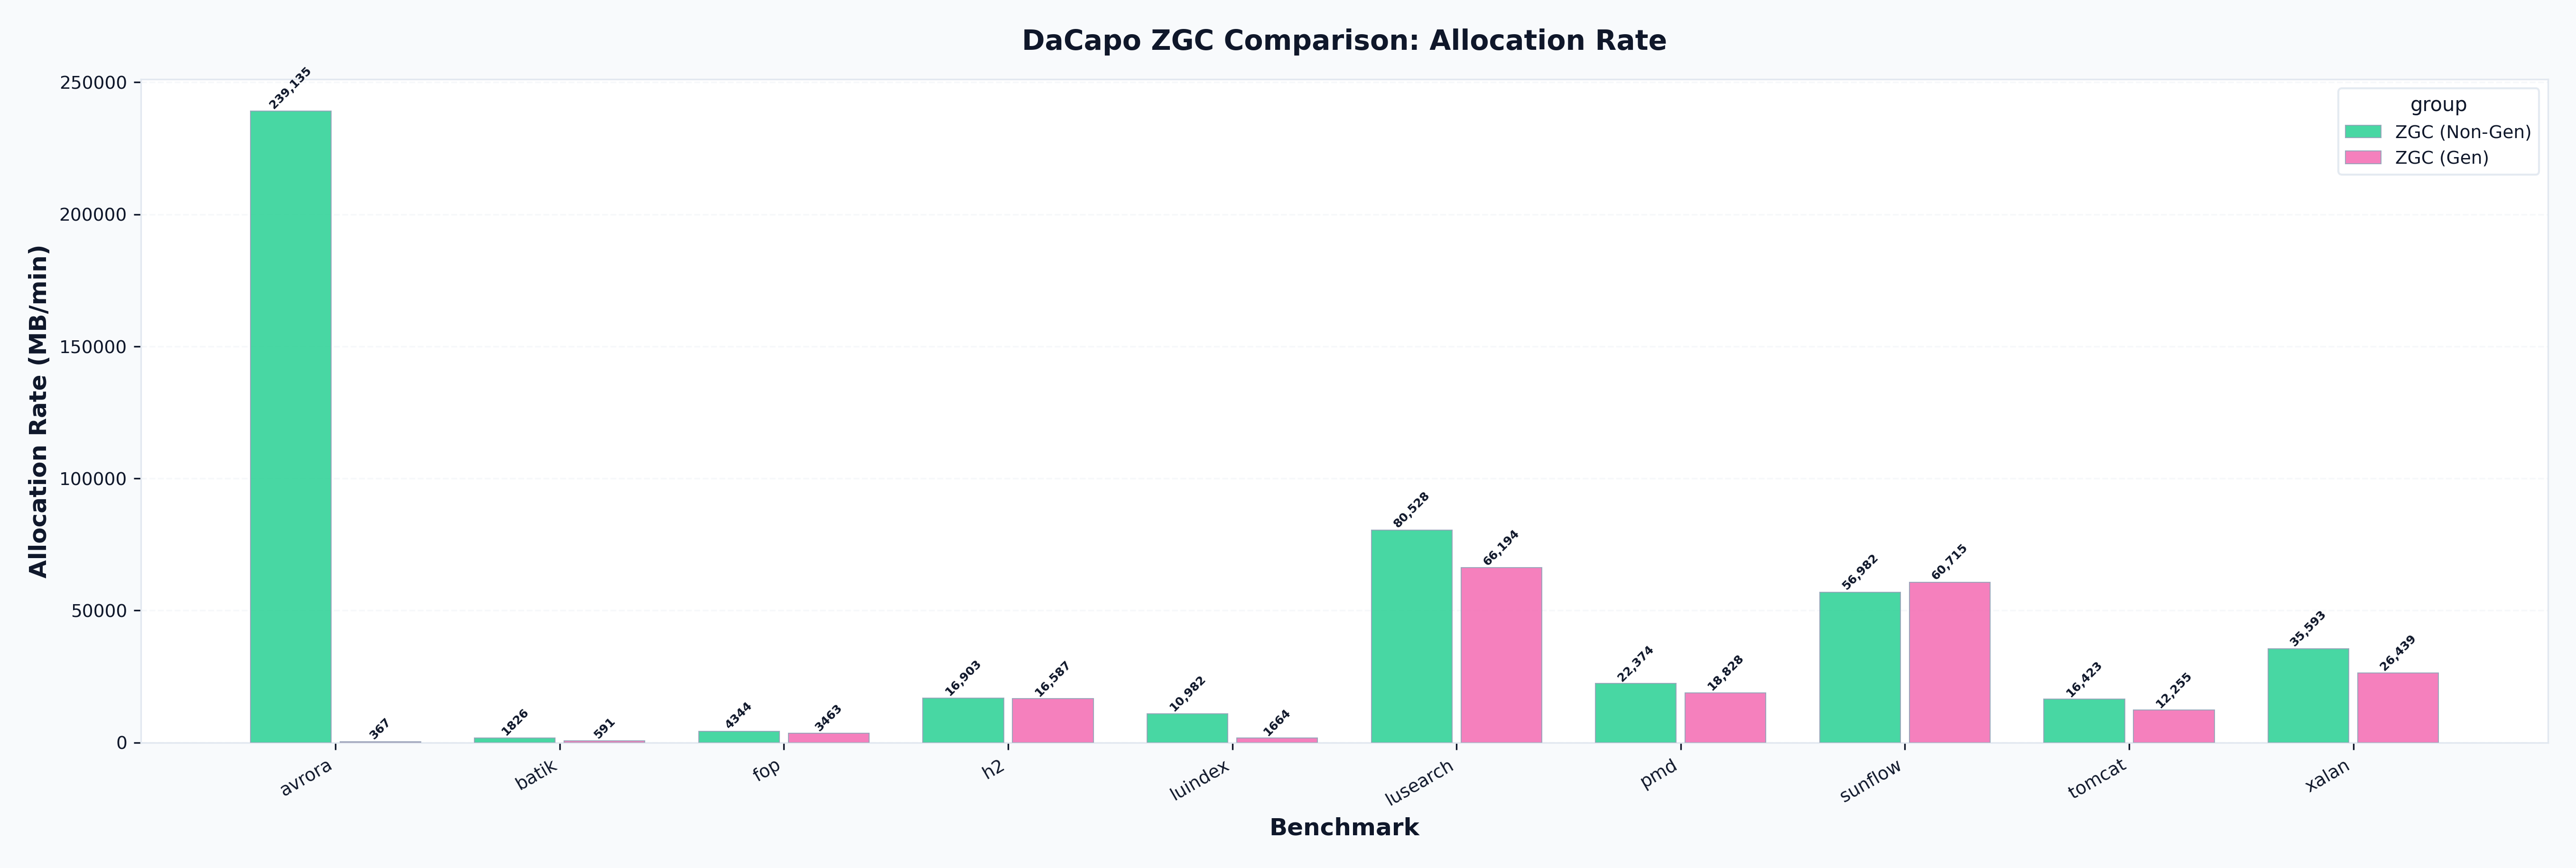
\includegraphics[width=\linewidth]{graphs/dacapo/zgc_comparison/dacapo_zgc_comparison_freedMemoryPerMin_zgc.png}
\caption{Freed Memory per Min}
\end{subfigure} &
\begin{subfigure}{0.45\textwidth}
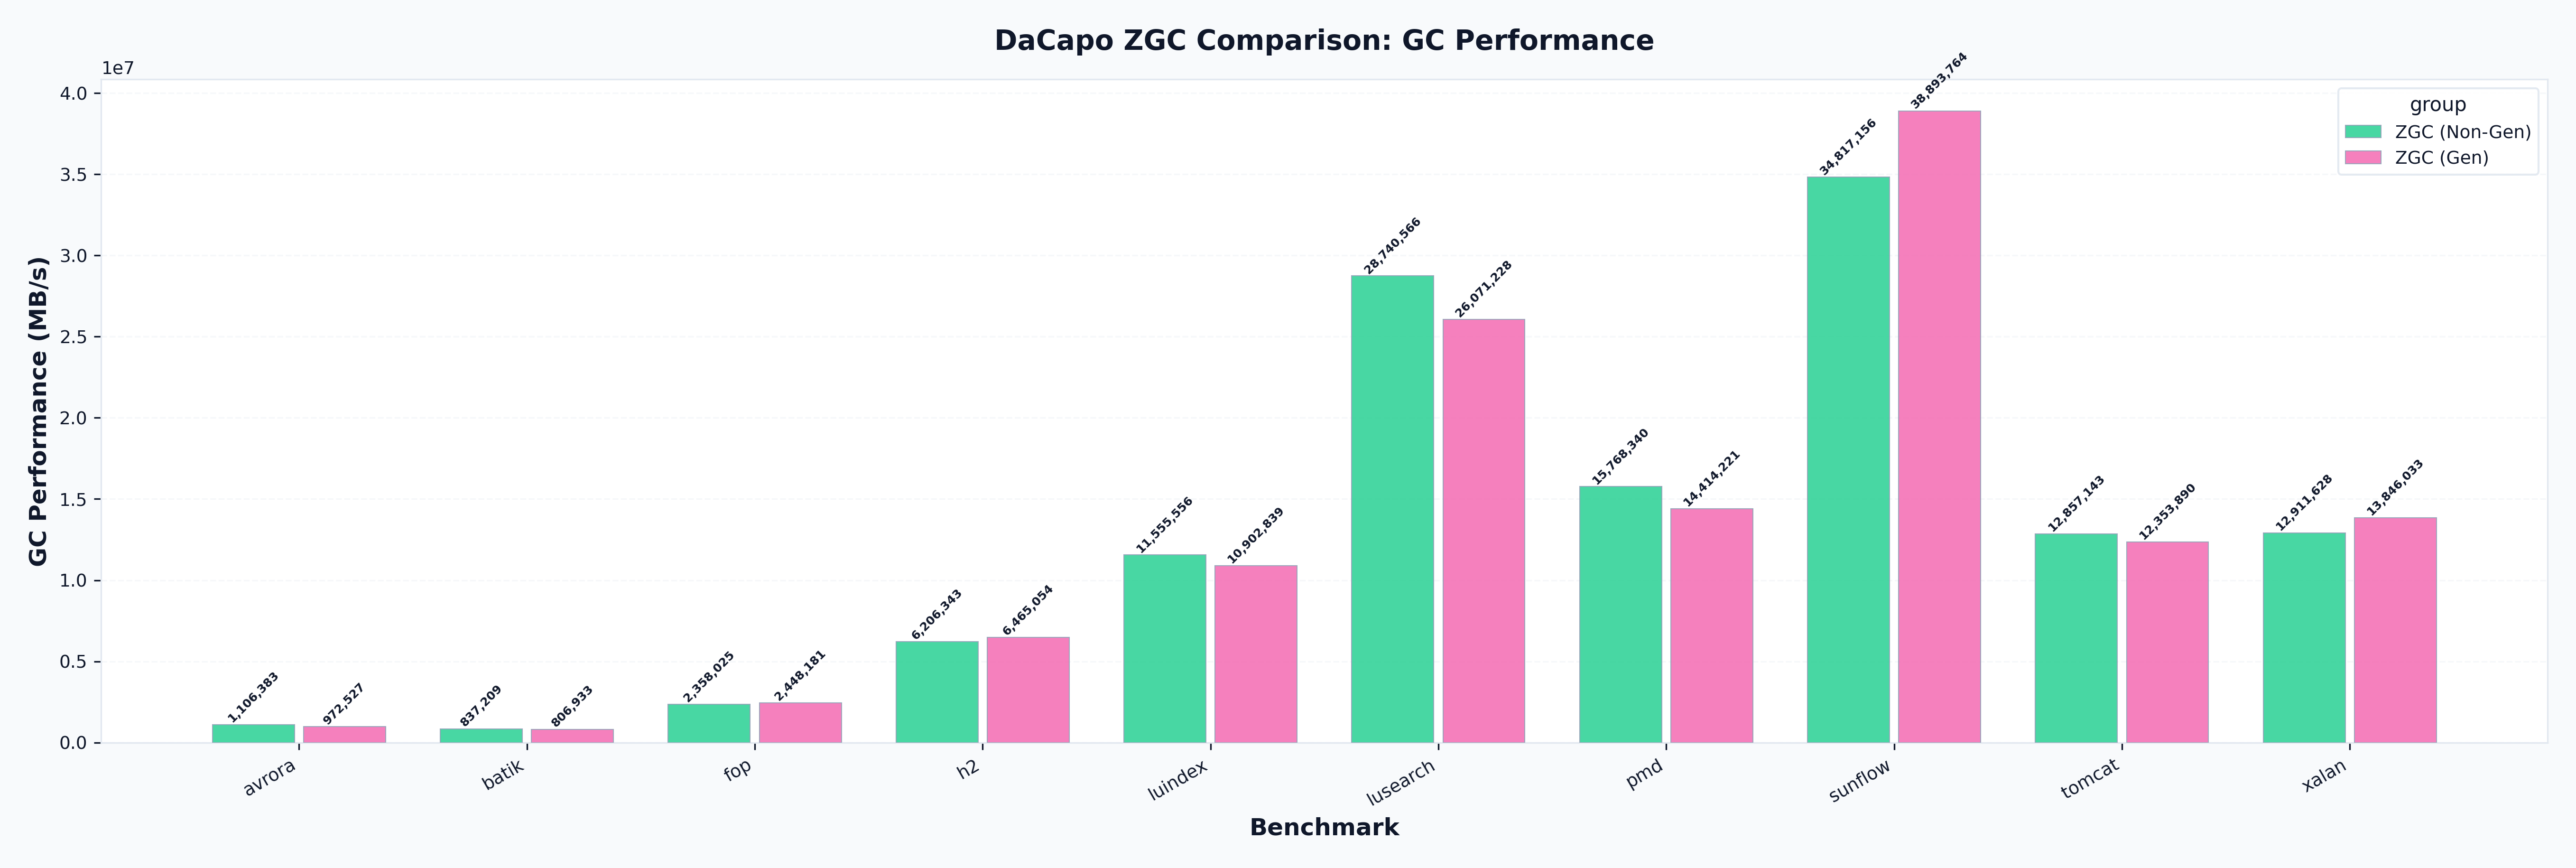
\includegraphics[width=\linewidth]{graphs/dacapo/zgc_comparison/dacapo_zgc_comparison_gcPerformance_zgc.png}
\caption{GC Performance}
\end{subfigure} \\

\begin{subfigure}{0.45\textwidth}
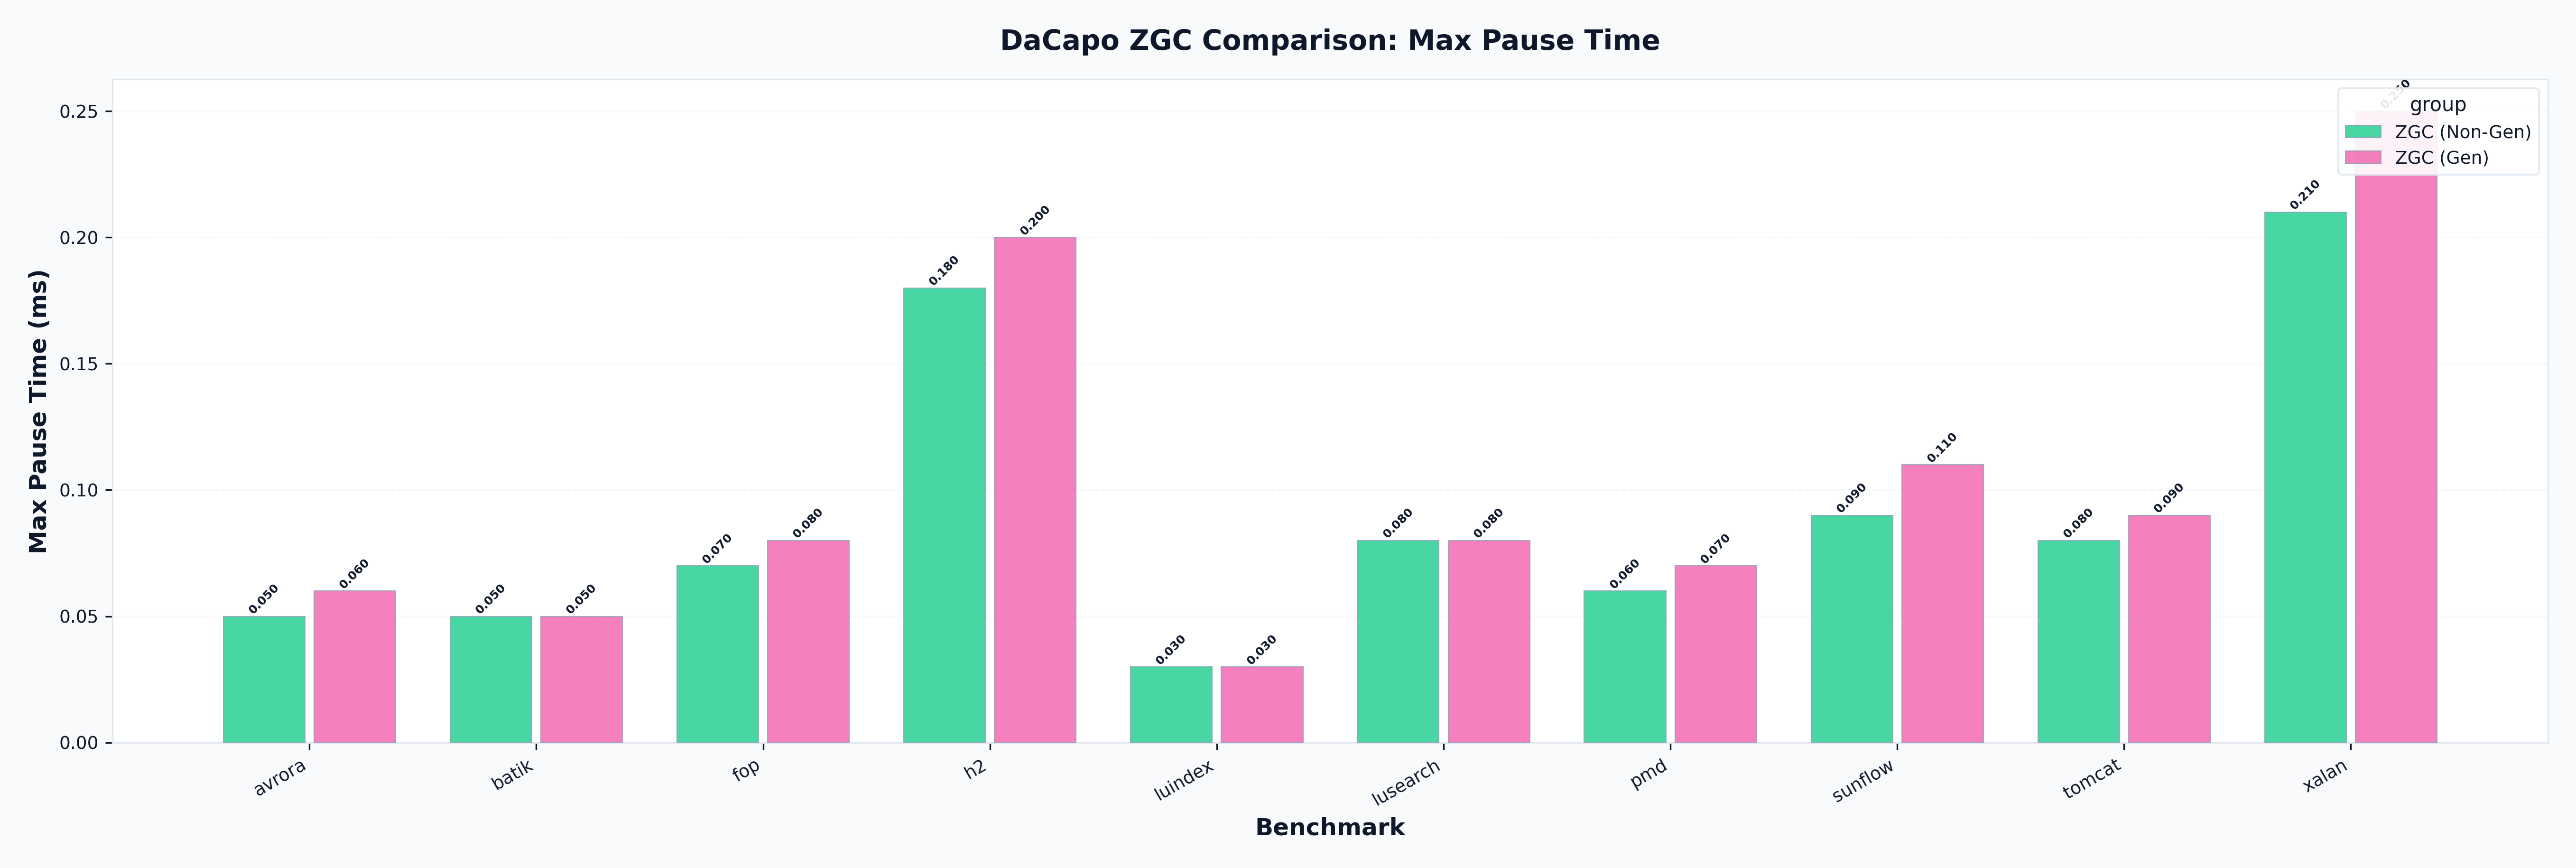
\includegraphics[width=\linewidth]{graphs/dacapo/zgc_comparison/dacapo_zgc_comparison_maxPause_zgc.png}
\caption{Max Pause}
\end{subfigure} &
\begin{subfigure}{0.45\textwidth}
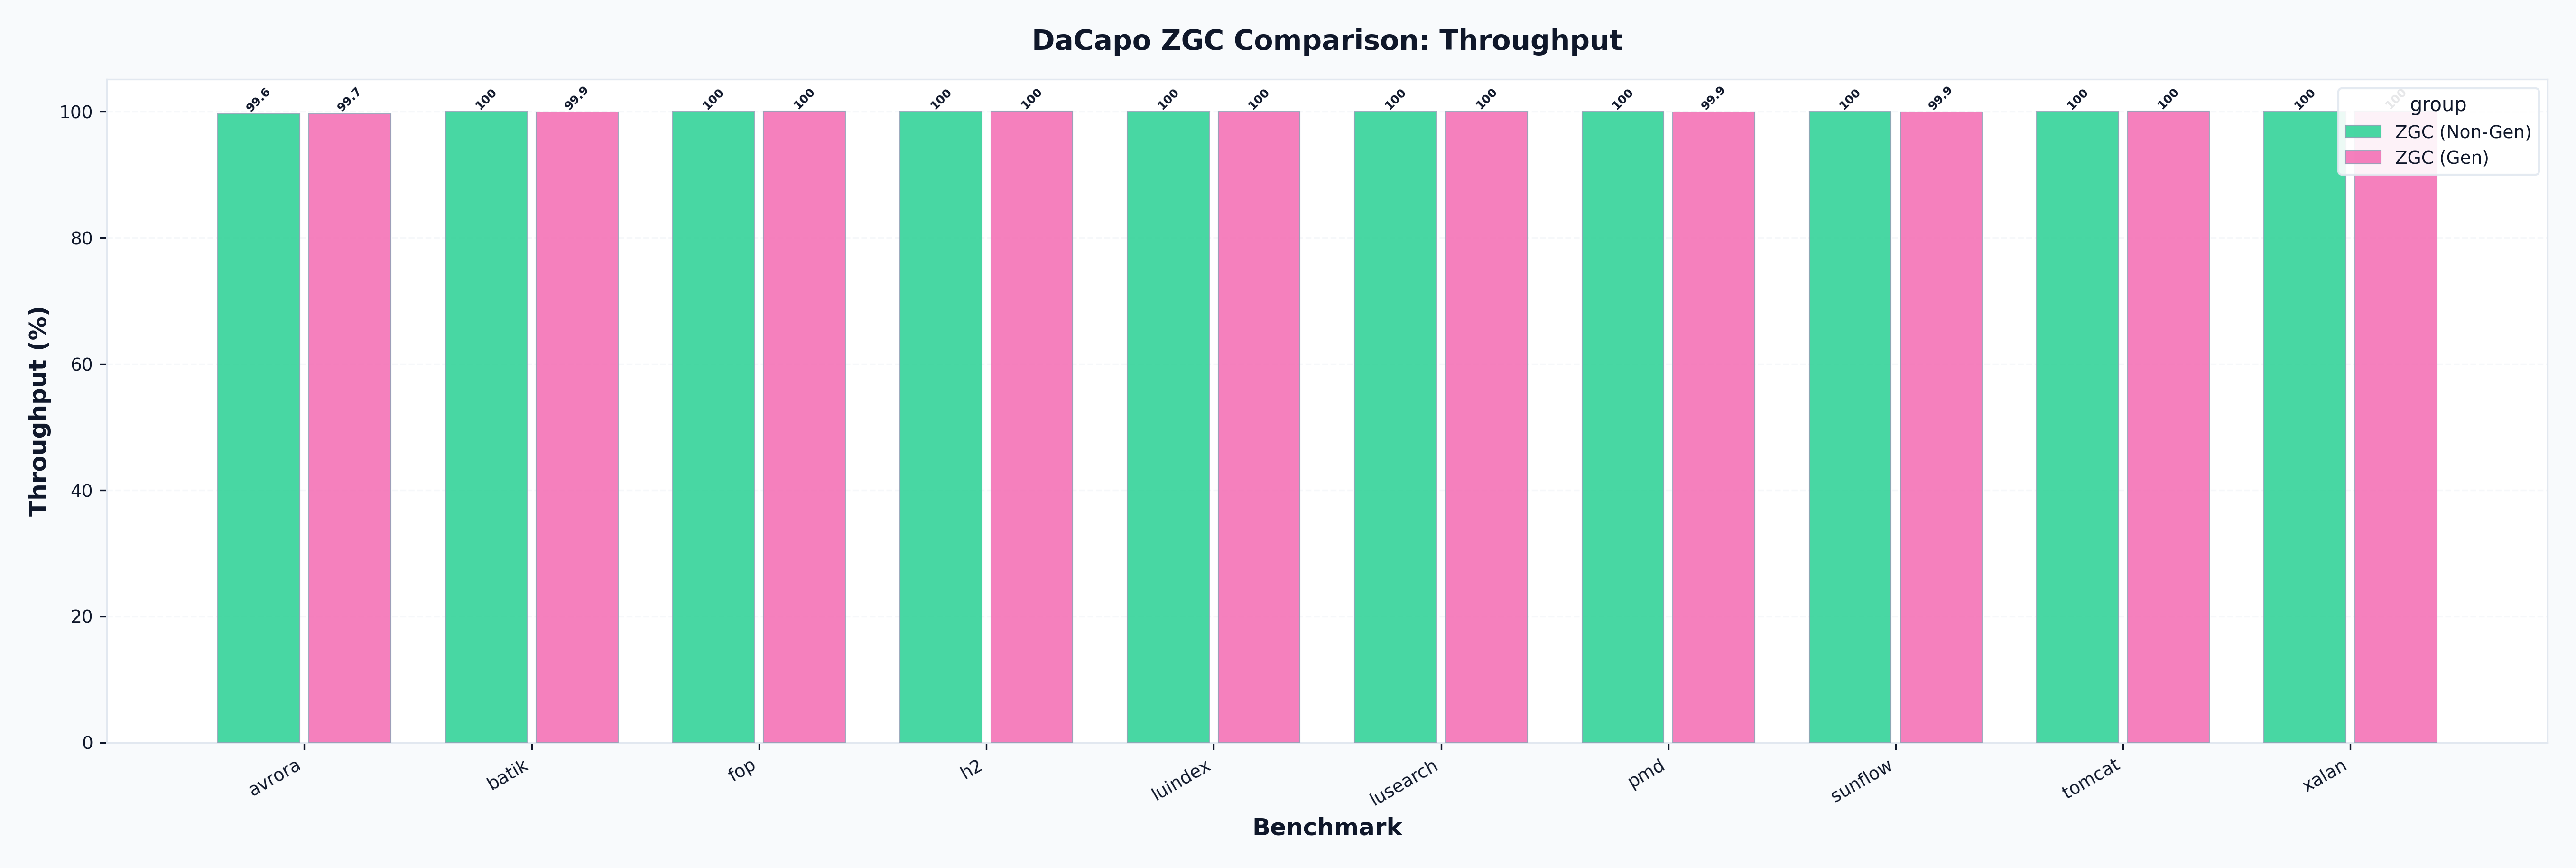
\includegraphics[width=\linewidth]{graphs/dacapo/zgc_comparison/dacapo_zgc_comparison_throughput_zgc.png}
\caption{Throughput}
\end{subfigure} \\

\begin{subfigure}{0.45\textwidth}
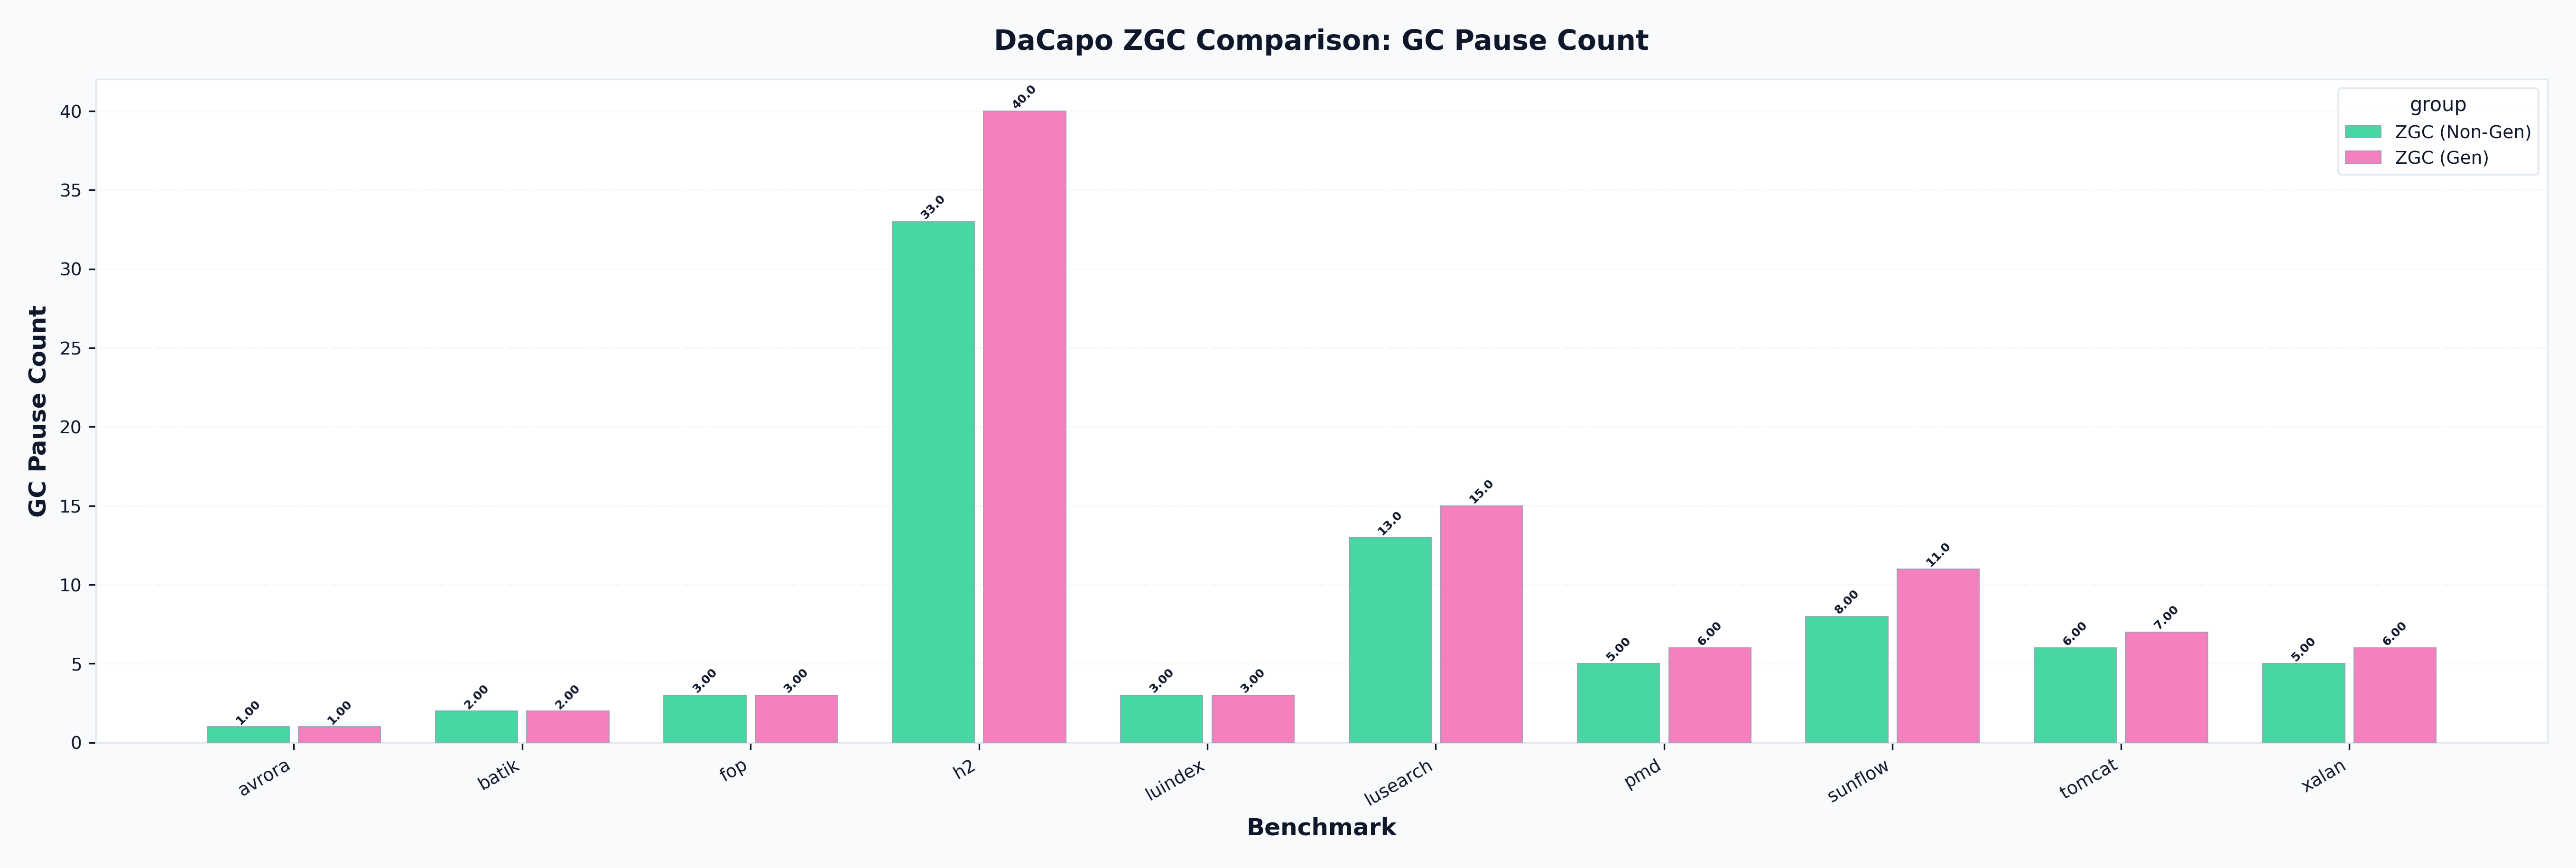
\includegraphics[width=\linewidth]{graphs/dacapo/zgc_comparison/dacapo_zgc_comparison_pauseCount_zgc.png}
\caption{Pause Count}
\end{subfigure} &
\begin{subfigure}{0.45\textwidth}
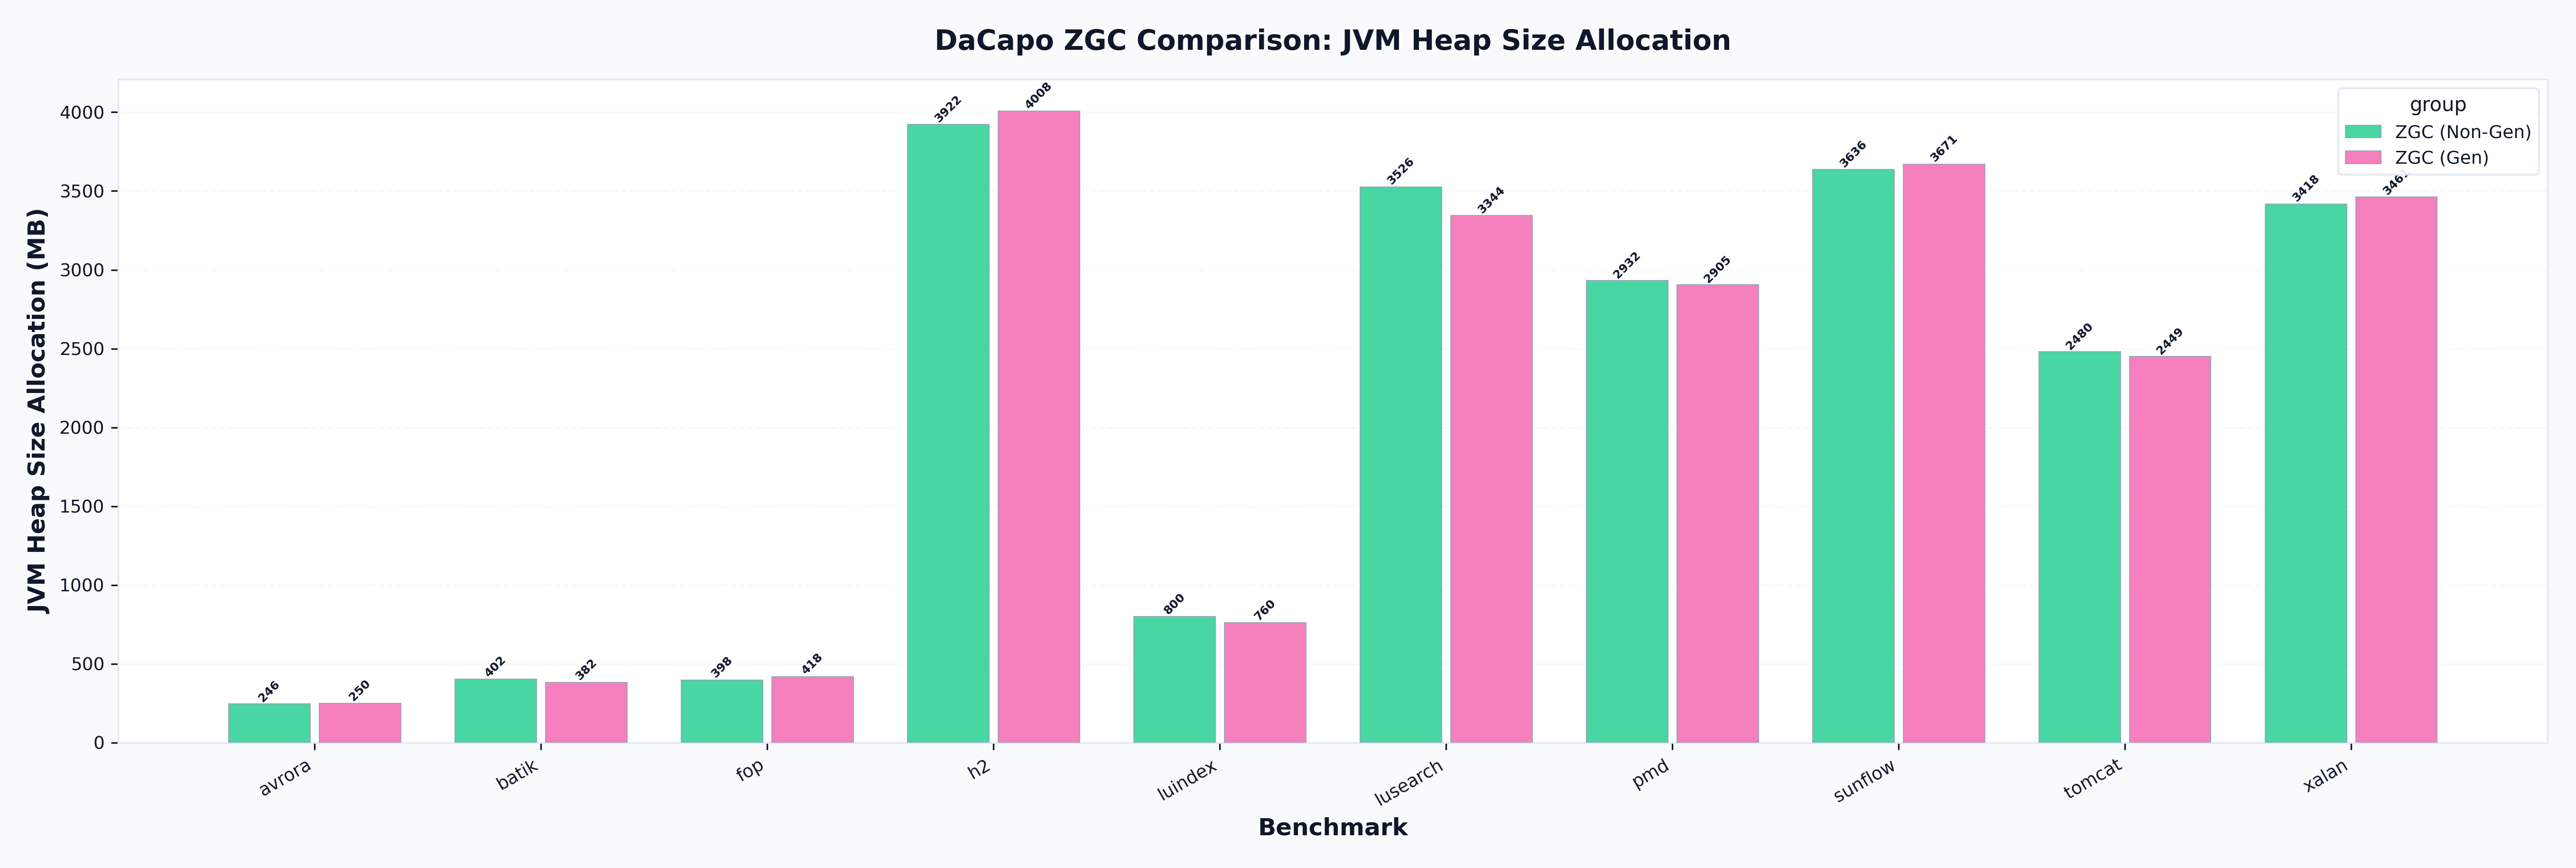
\includegraphics[width=\linewidth]{graphs/dacapo/zgc_comparison/dacapo_zgc_comparison_totalHeapAllocMax_zgc.png}
\caption{Total Heap Alloc Max}
\end{subfigure} \\

\begin{subfigure}{0.45\textwidth}
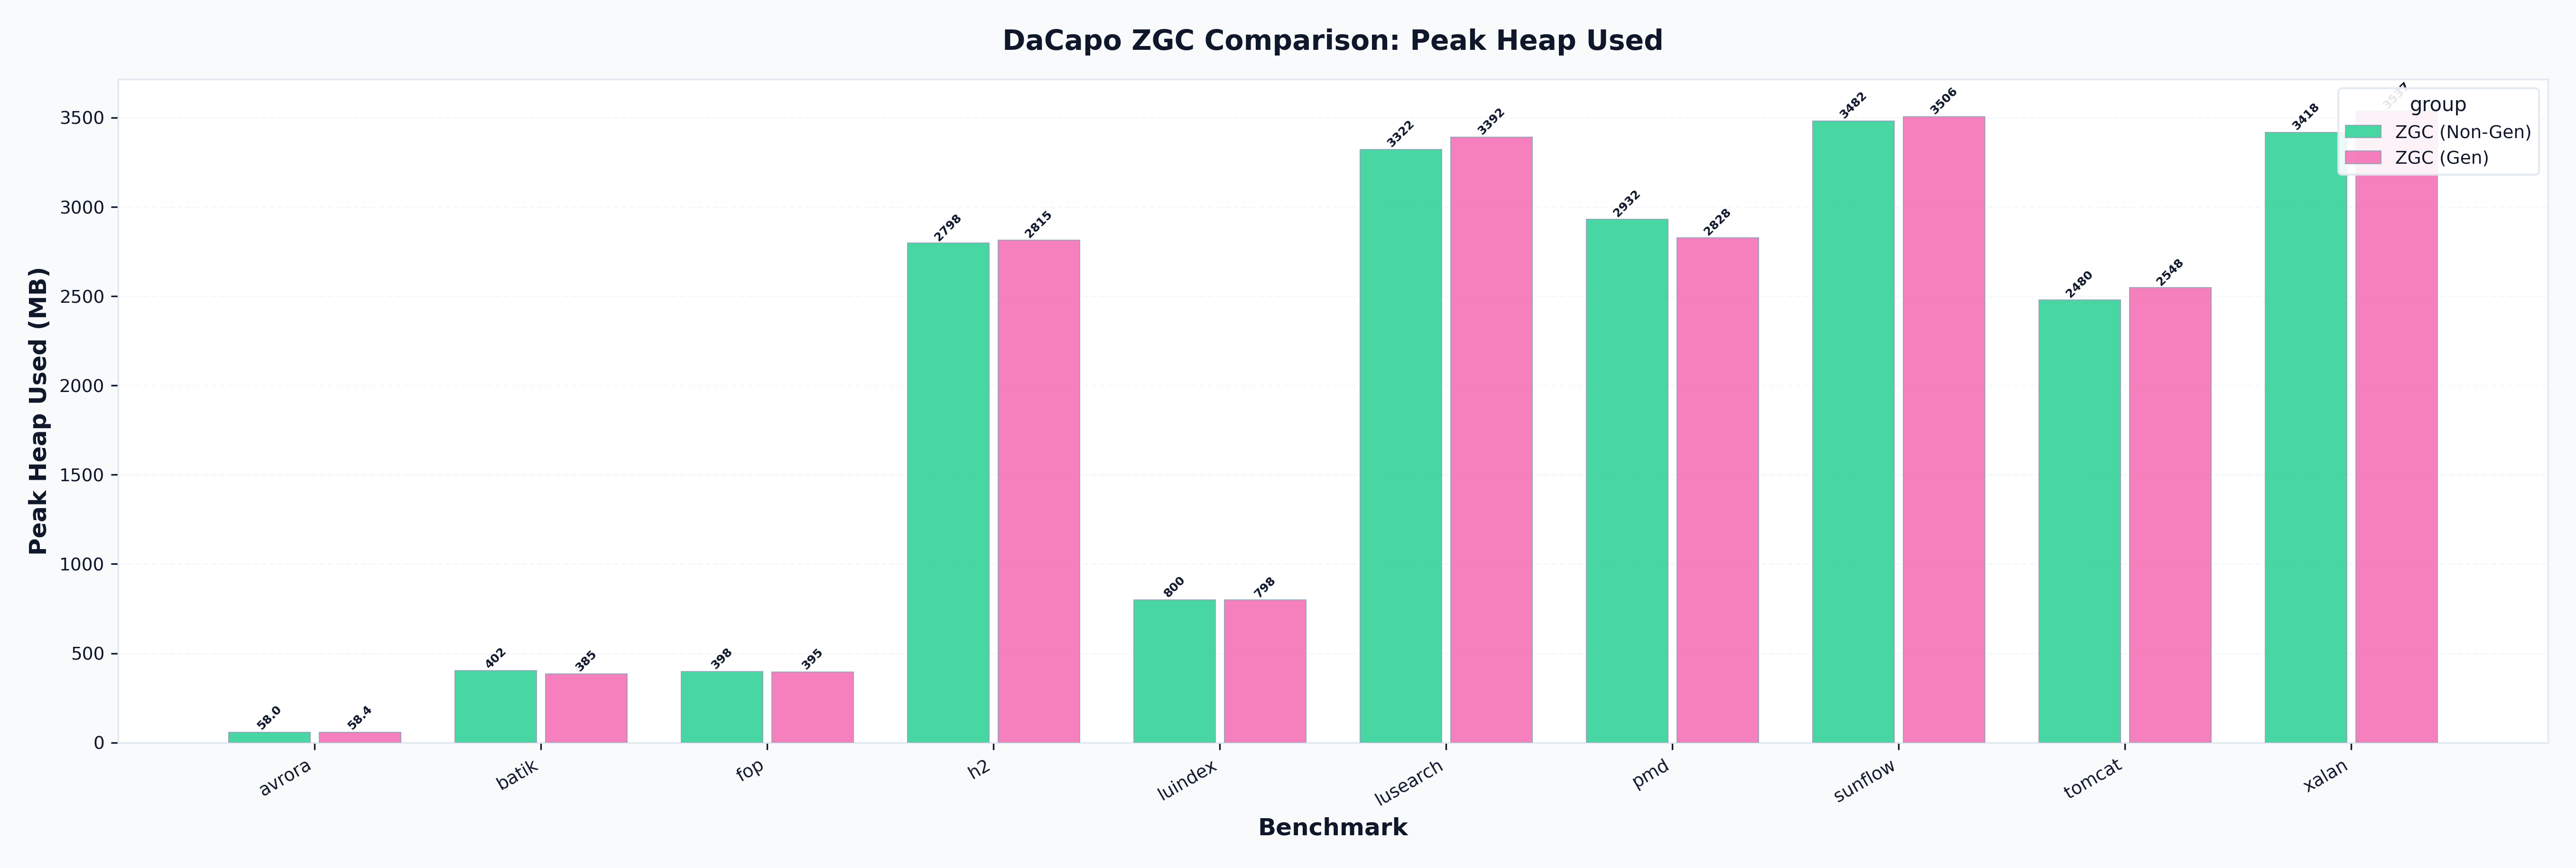
\includegraphics[width=\linewidth]{graphs/dacapo/zgc_comparison/dacapo_zgc_comparison_totalHeapUsedMax_zgc.png}
\caption{Total Heap Used Max}
\end{subfigure} &
\begin{subfigure}{0.45\textwidth}
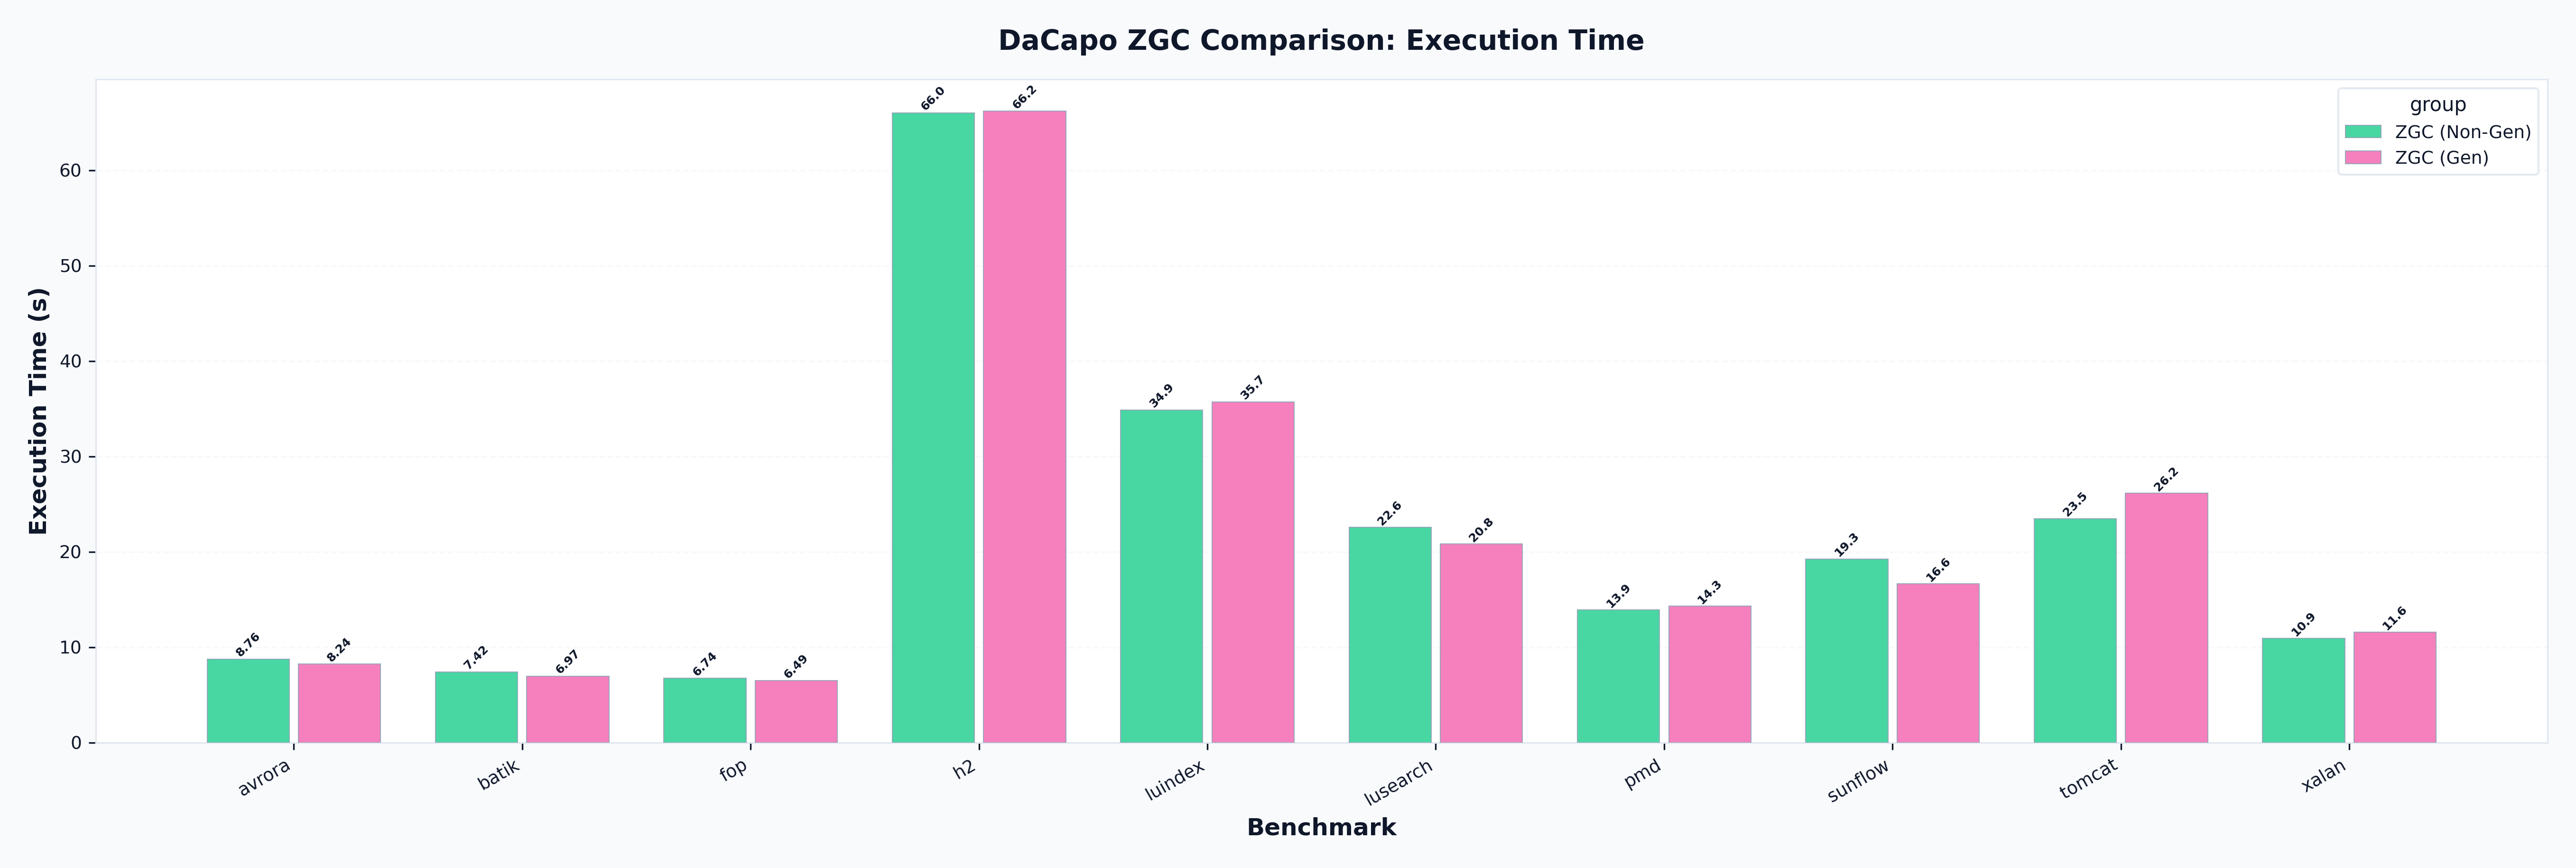
\includegraphics[width=\linewidth]{graphs/dacapo/zgc_comparison/dacapo_zgc_comparison_wallTimeSec_zgc.png}
\caption{Wall Time (sec)}
\end{subfigure} \\

\end{tabular}

\caption{ZGC Comparison Across DaCapo Benchmarks Using Different Metrics}
\label{fig:dacapo_zgc_comparison}
\end{figure}

\begin{figure}[h]
\centering

\begin{tabular}{cc}

\begin{subfigure}{0.45\textwidth}
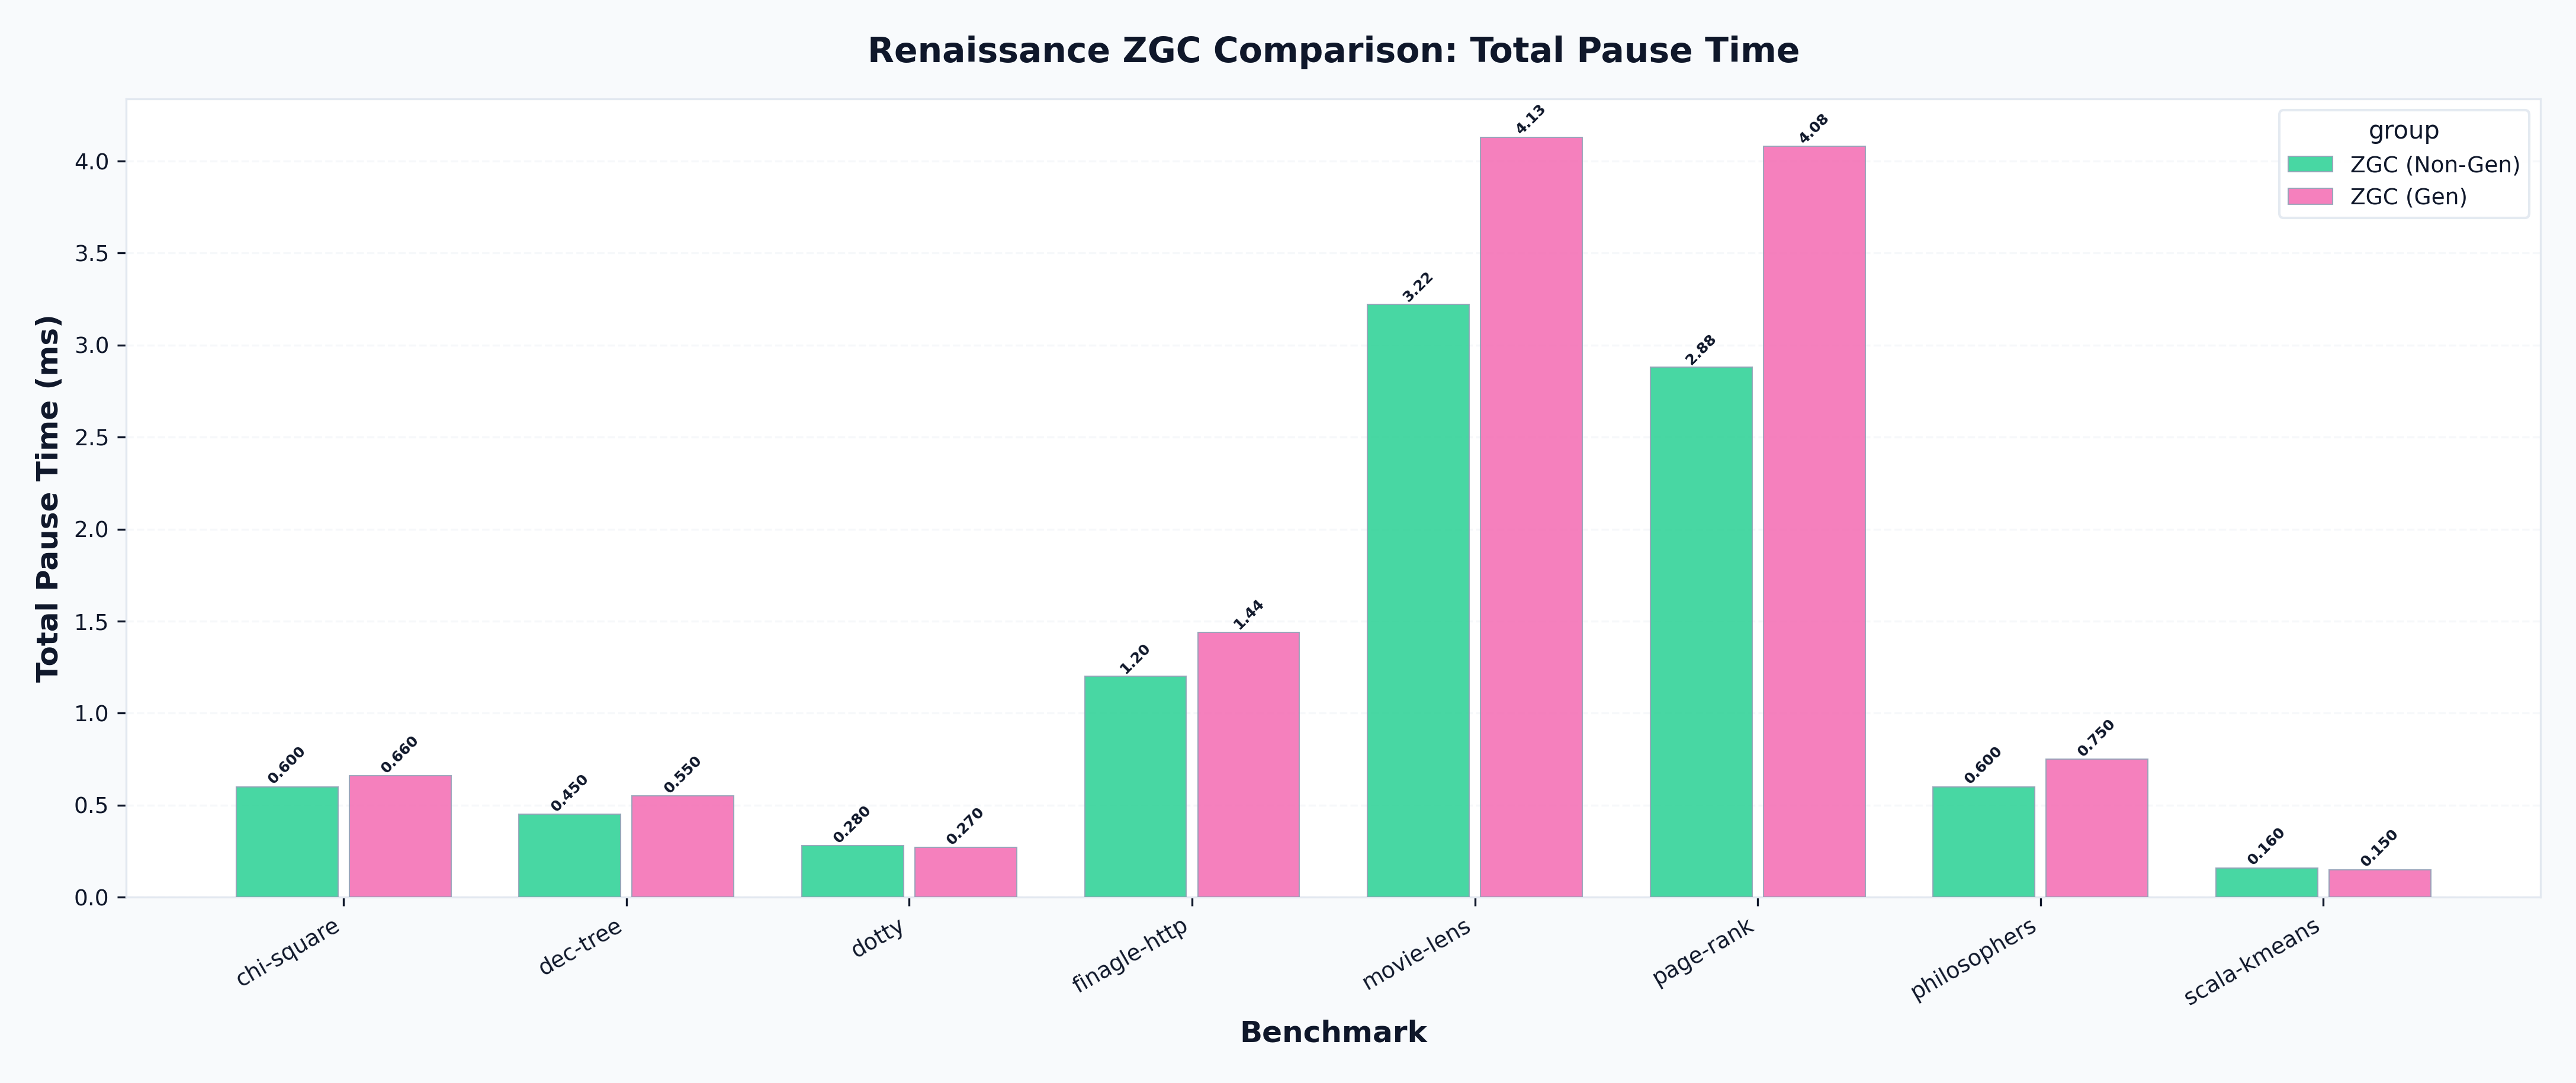
\includegraphics[width=\linewidth]{graphs/renaissance/zgc_comparison/renaissance_zgc_comparison_accumPause_zgc.png}
\caption{Accumulated Pause}
\end{subfigure} &
\begin{subfigure}{0.45\textwidth}
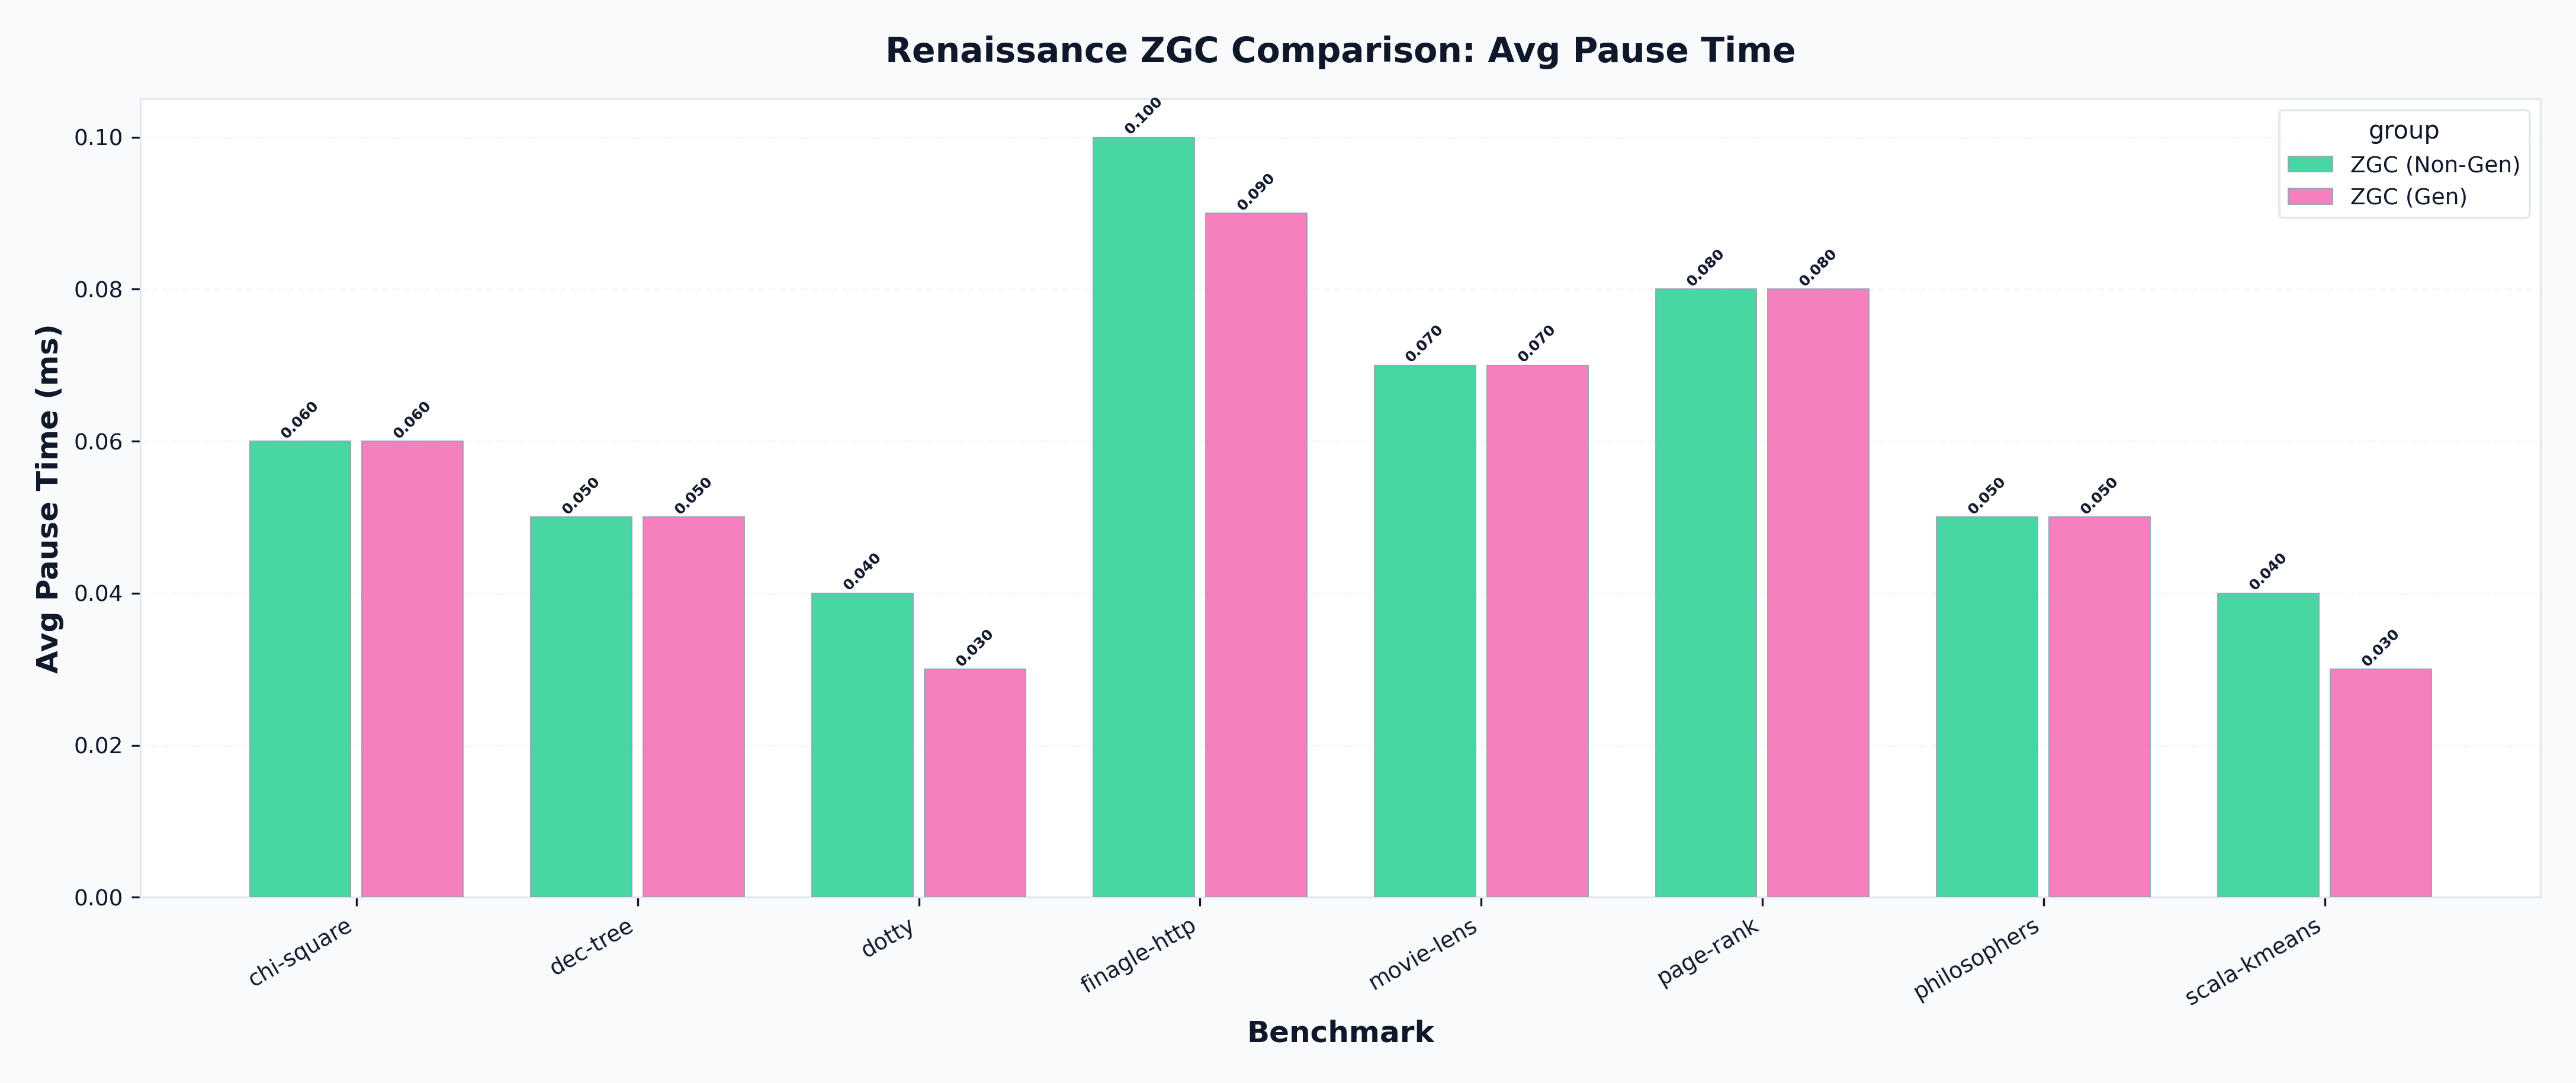
\includegraphics[width=\linewidth]{graphs/renaissance/zgc_comparison/renaissance_zgc_comparison_avgPause_zgc.png}
\caption{Average Pause}
\end{subfigure} \\

\begin{subfigure}{0.45\textwidth}
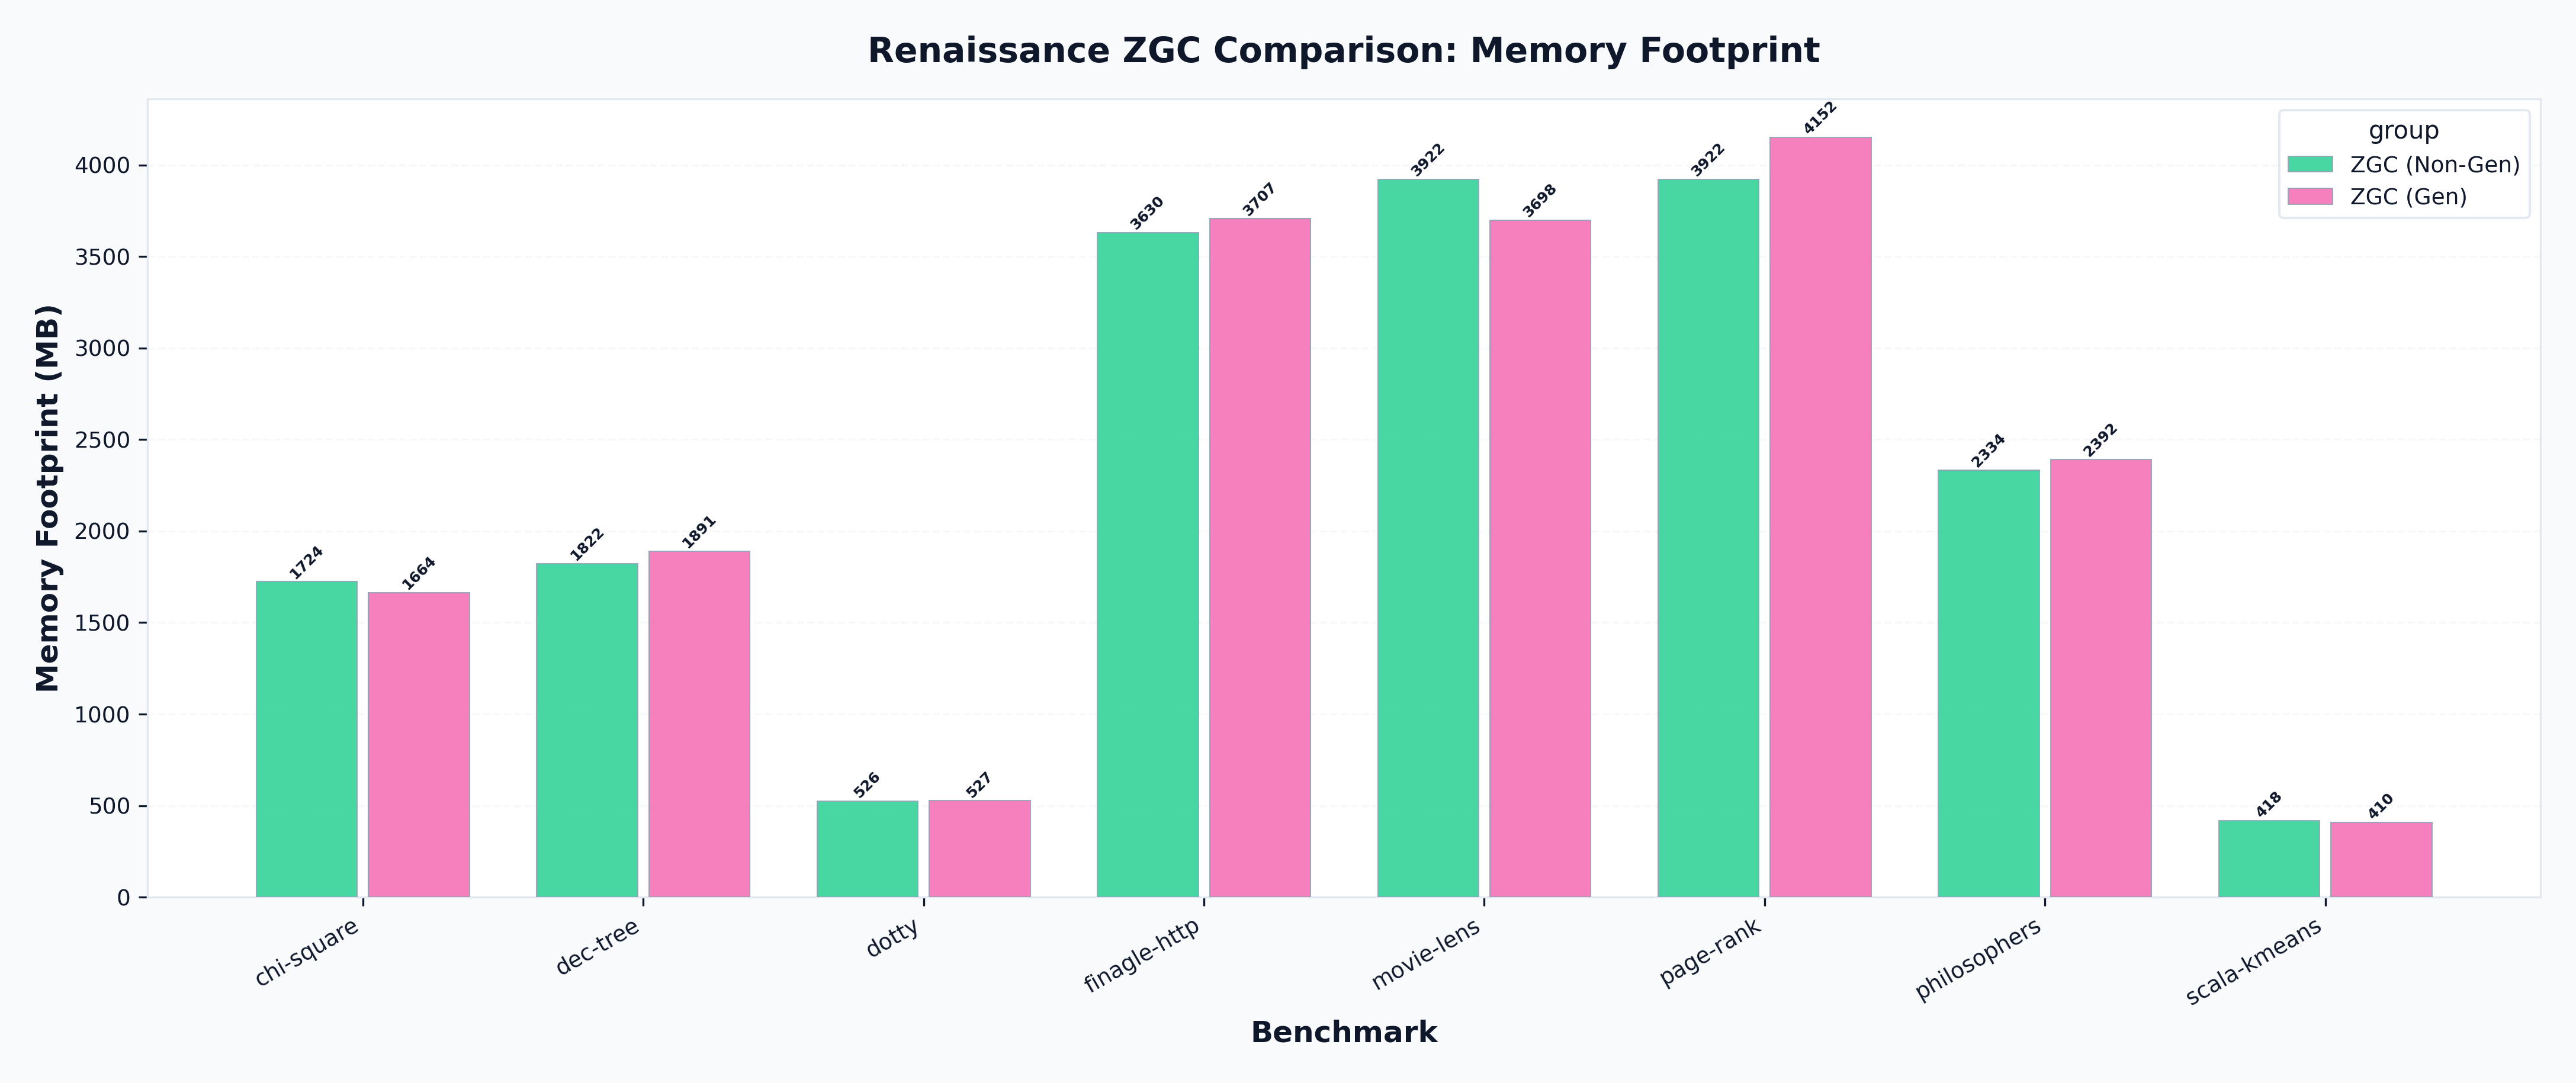
\includegraphics[width=\linewidth]{graphs/renaissance/zgc_comparison/renaissance_zgc_comparison_footprint_zgc.png}
\caption{Footprint}
\end{subfigure} &
\begin{subfigure}{0.45\textwidth}
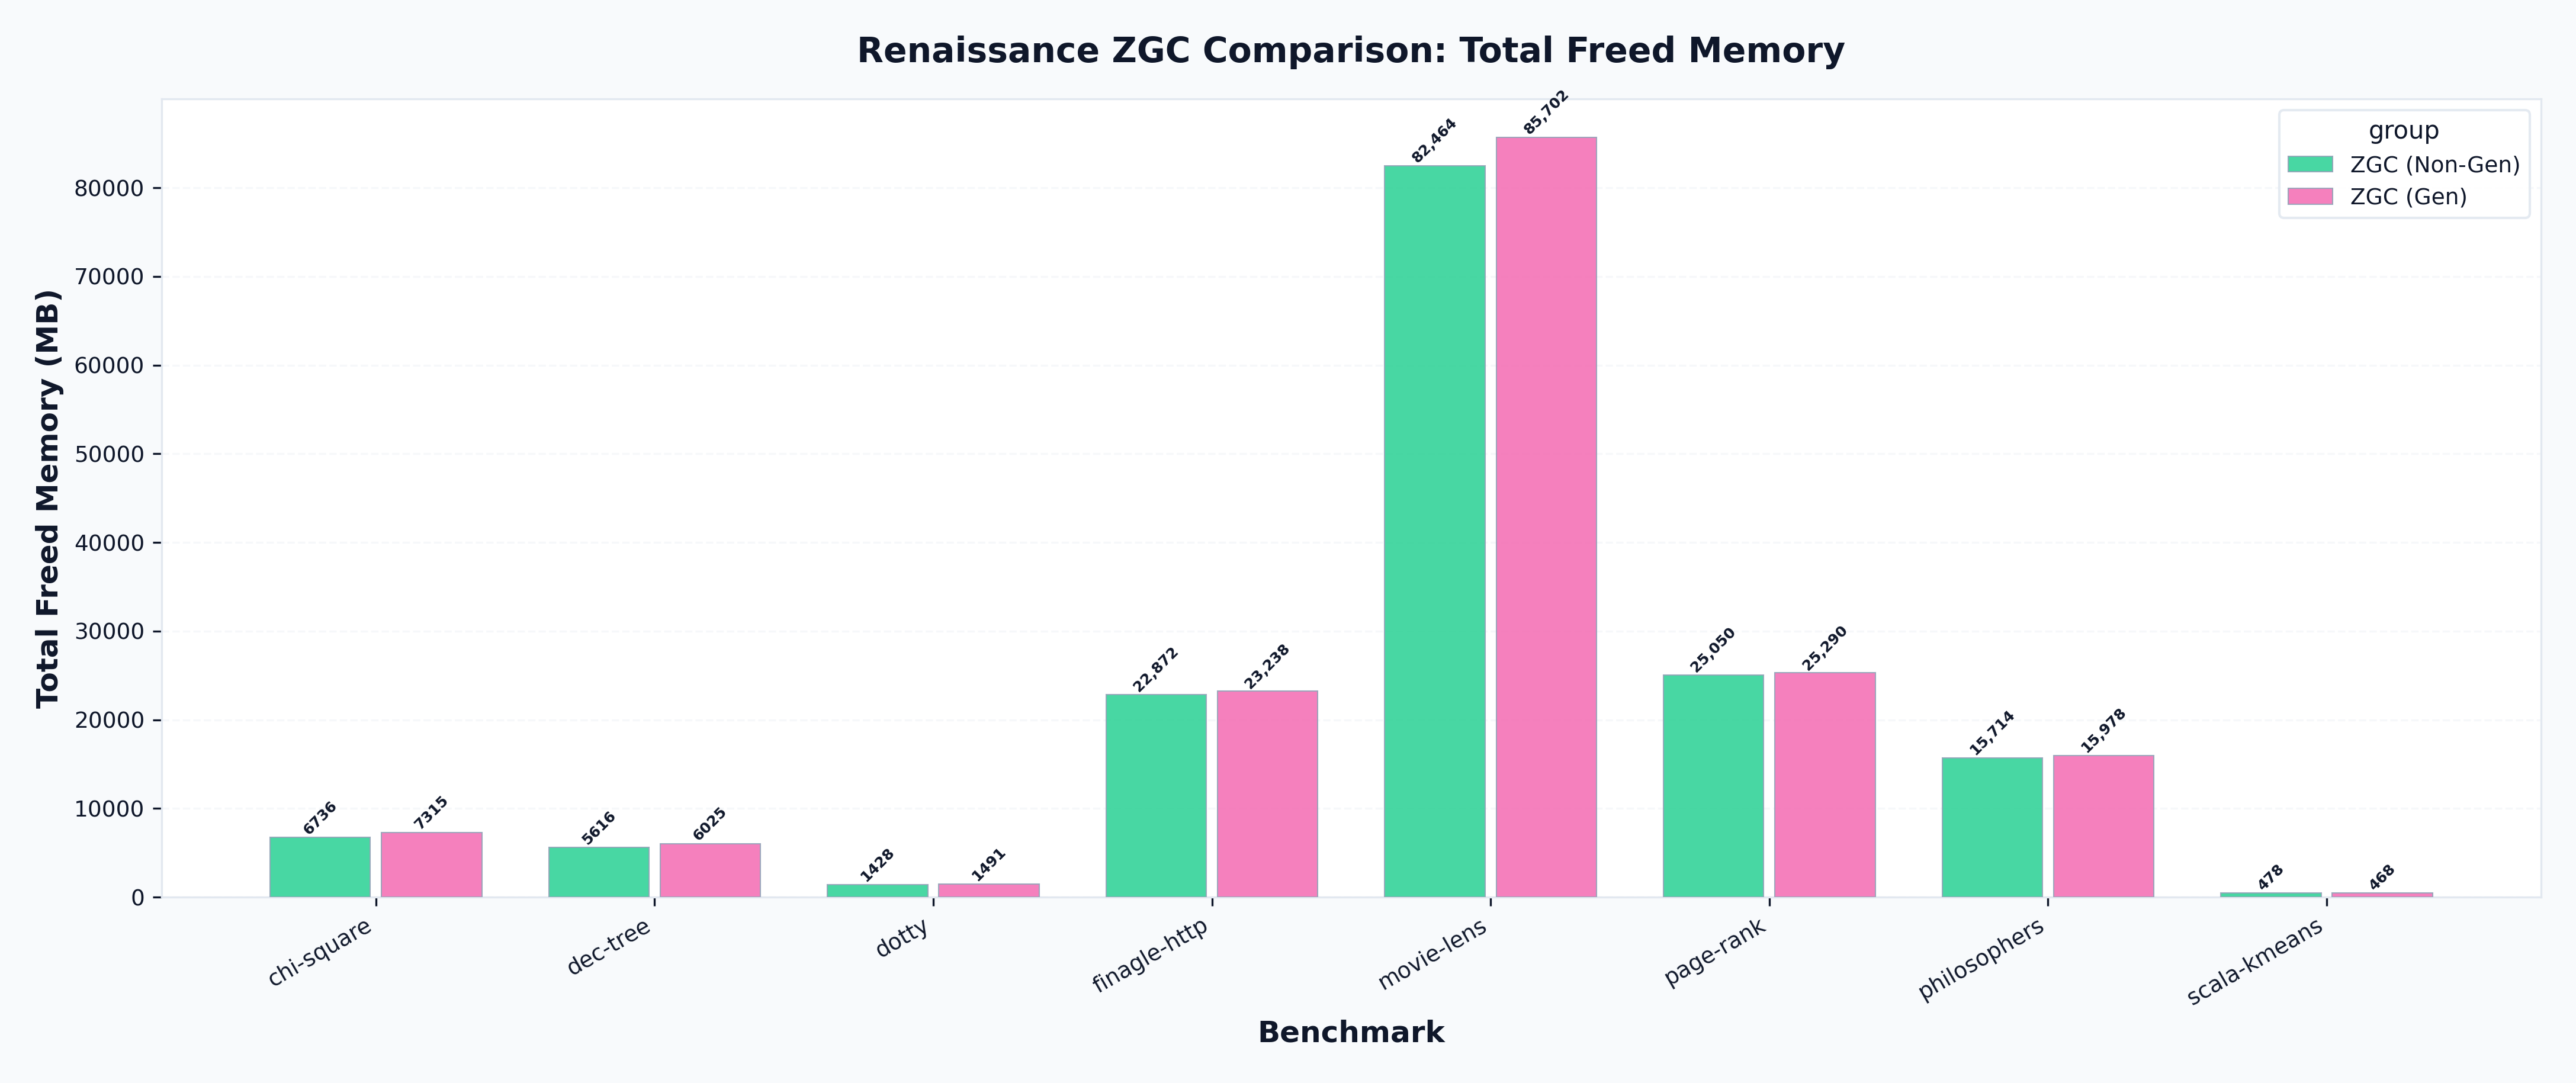
\includegraphics[width=\linewidth]{graphs/renaissance/zgc_comparison/renaissance_zgc_comparison_freedMemory_zgc.png}
\caption{Freed Memory}
\end{subfigure} \\

\begin{subfigure}{0.45\textwidth}
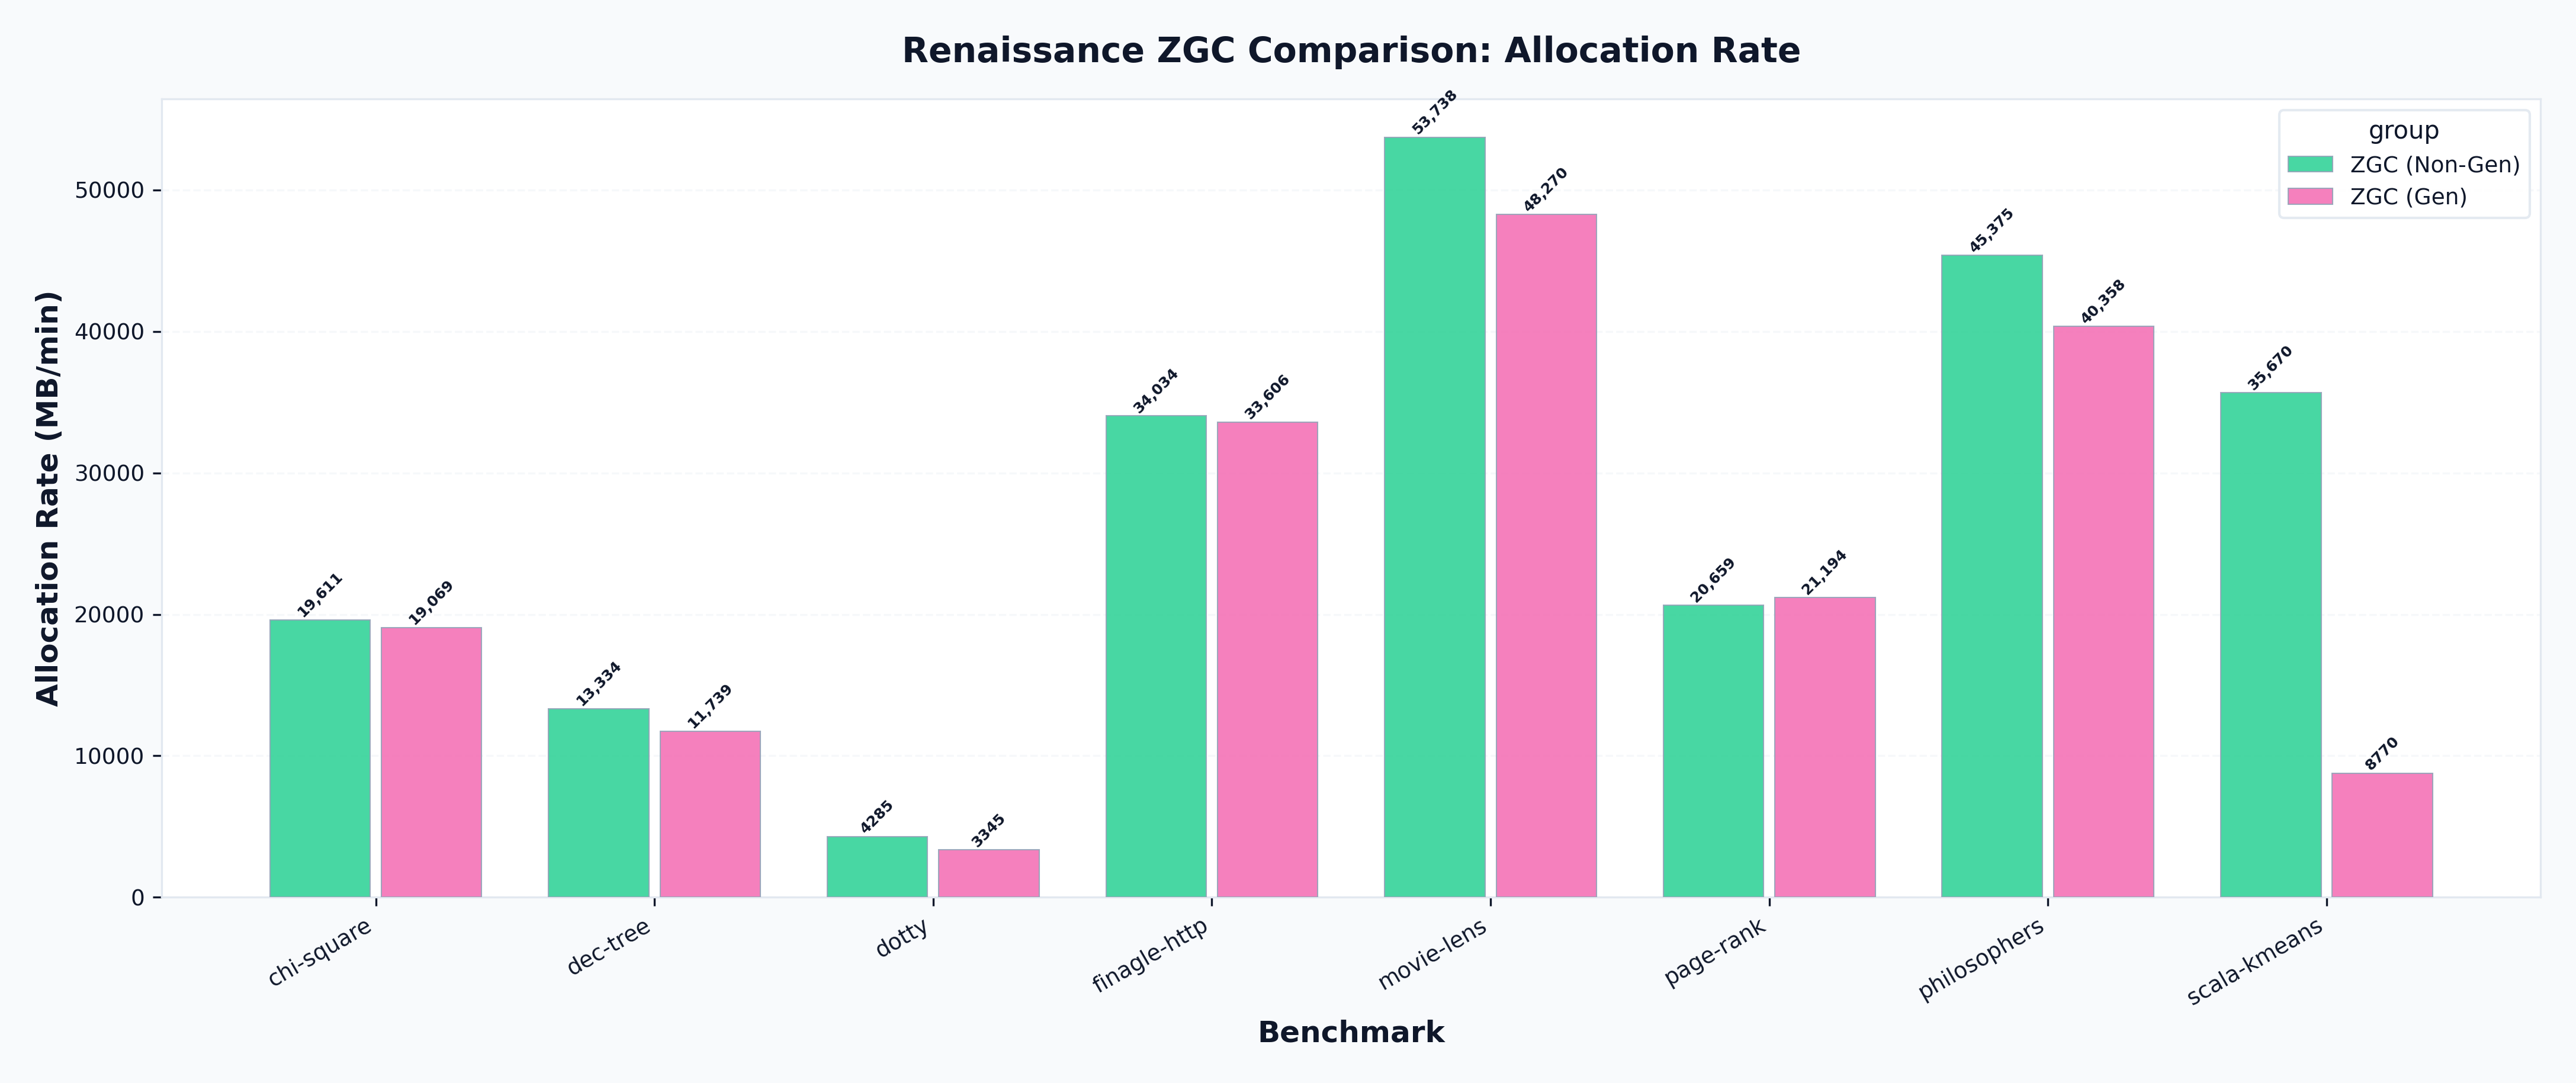
\includegraphics[width=\linewidth]{graphs/renaissance/zgc_comparison/renaissance_zgc_comparison_freedMemoryPerMin_zgc.png}
\caption{Freed Memory per Min}
\end{subfigure} &
\begin{subfigure}{0.45\textwidth}
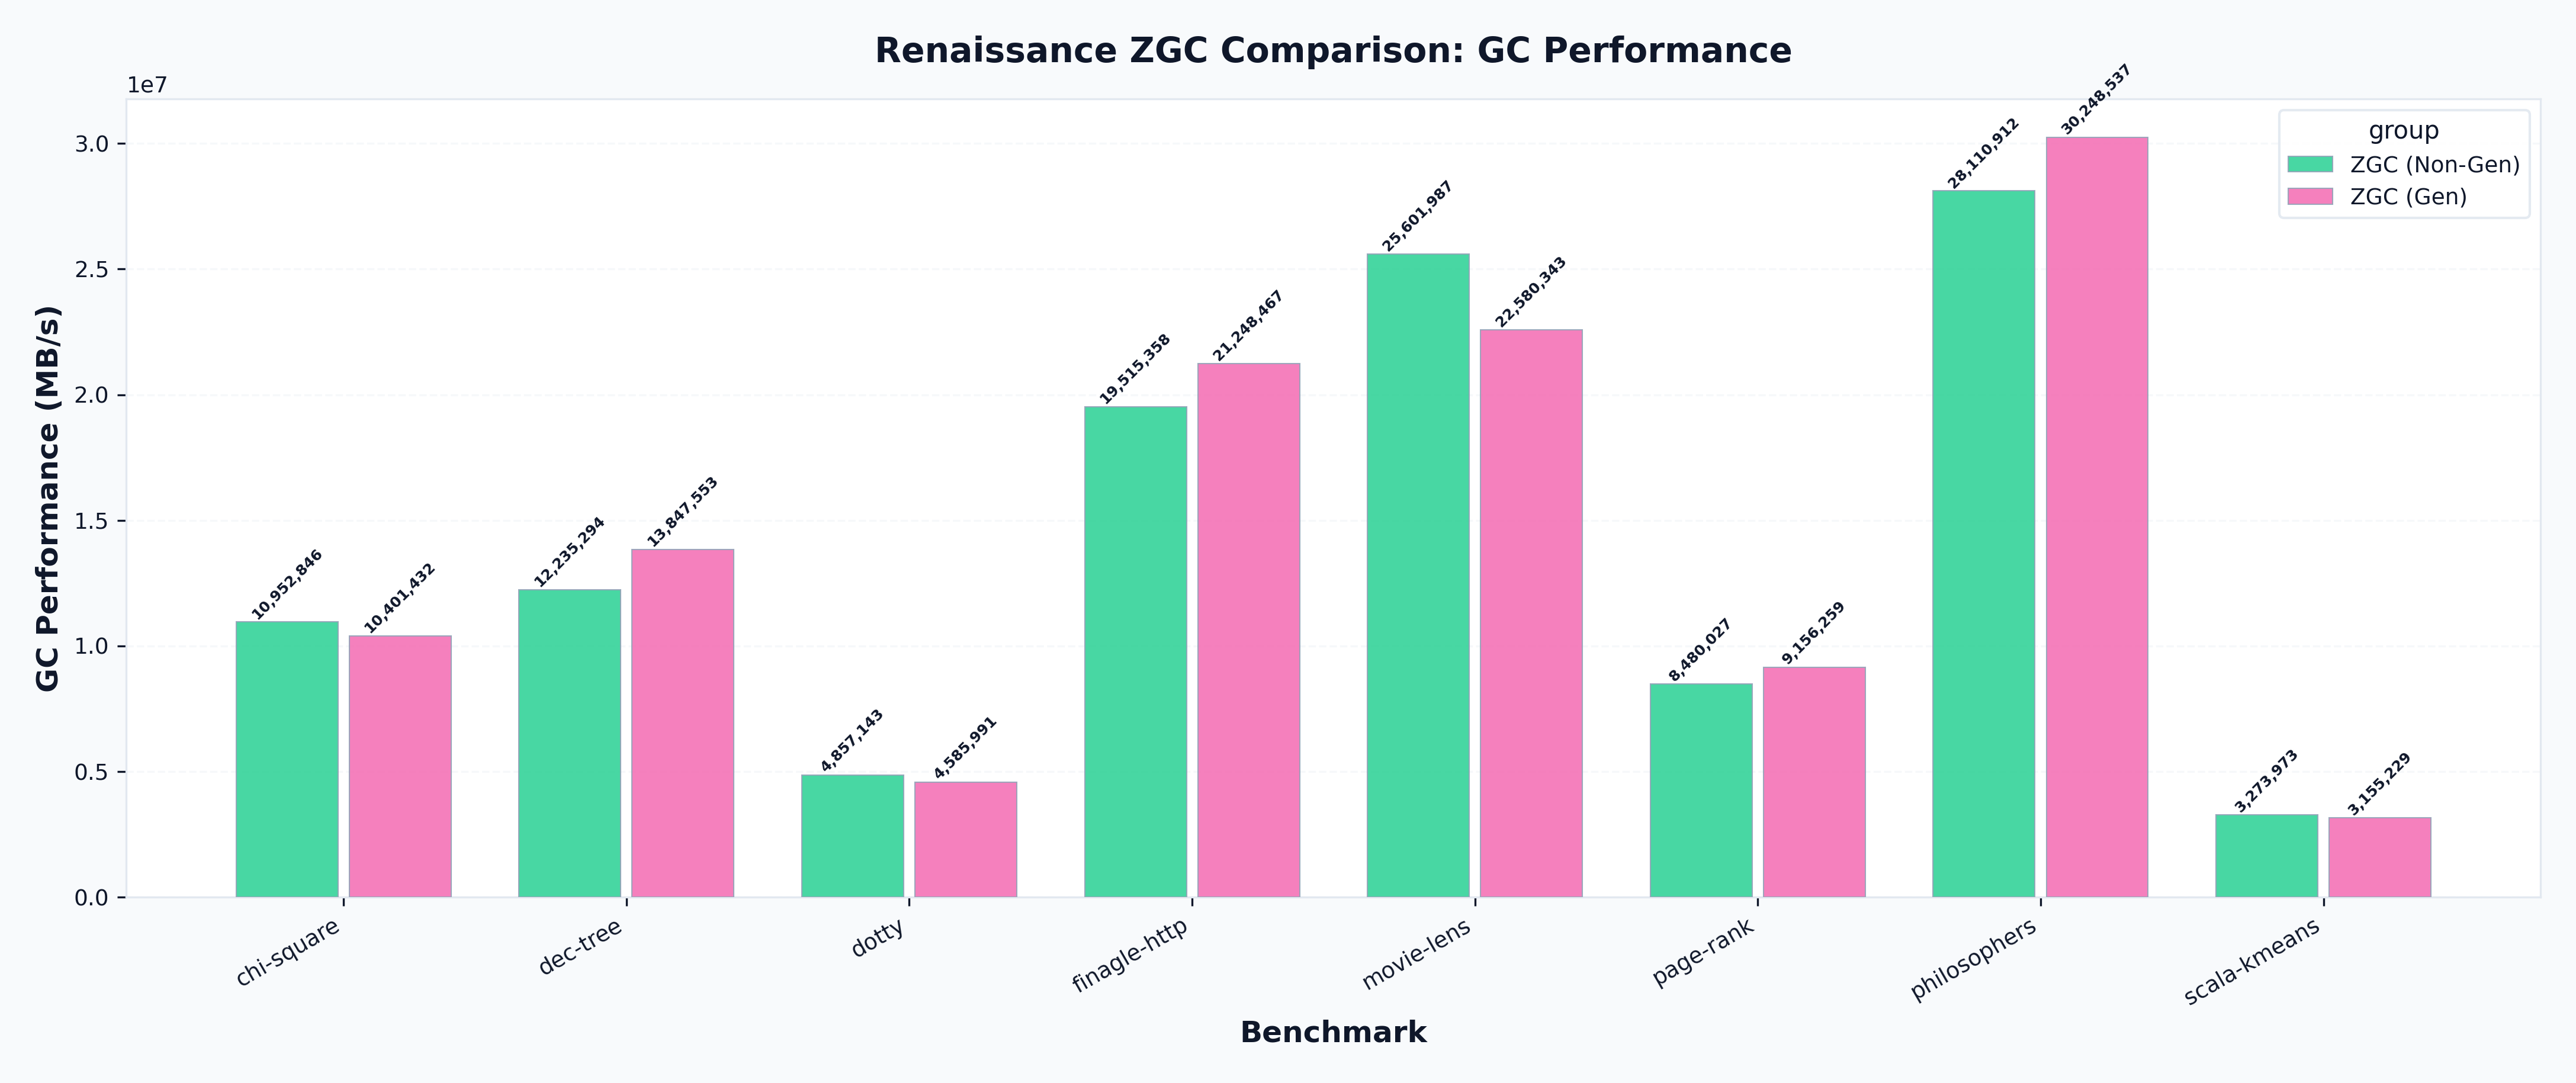
\includegraphics[width=\linewidth]{graphs/renaissance/zgc_comparison/renaissance_zgc_comparison_gcPerformance_zgc.png}
\caption{GC Performance}
\end{subfigure} \\

\begin{subfigure}{0.45\textwidth}
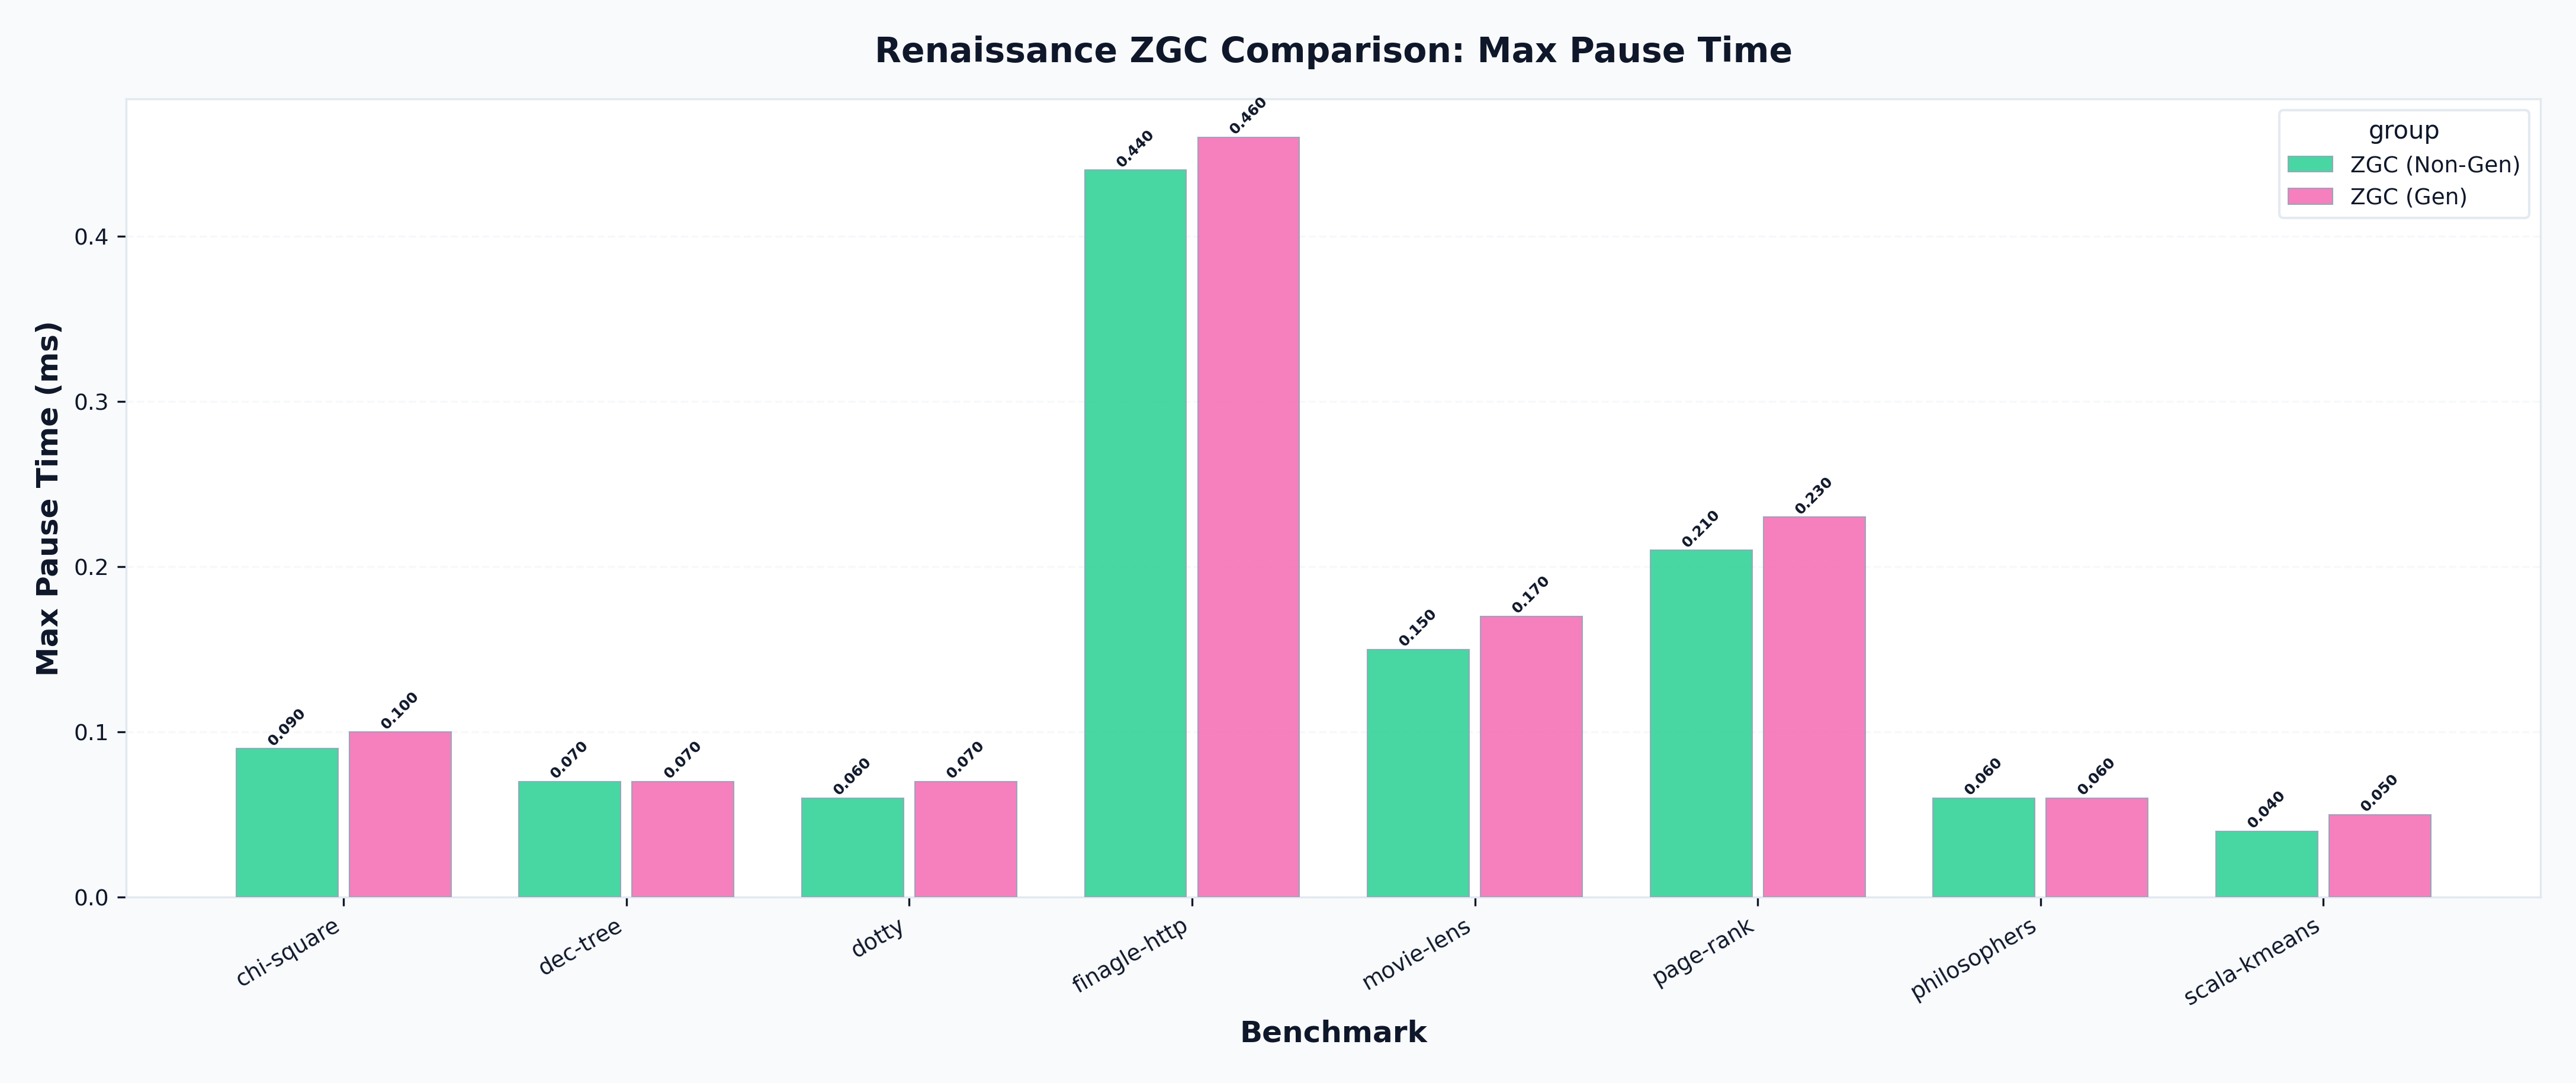
\includegraphics[width=\linewidth]{graphs/renaissance/zgc_comparison/renaissance_zgc_comparison_maxPause_zgc.png}
\caption{Max Pause}
\end{subfigure} &
\begin{subfigure}{0.45\textwidth}
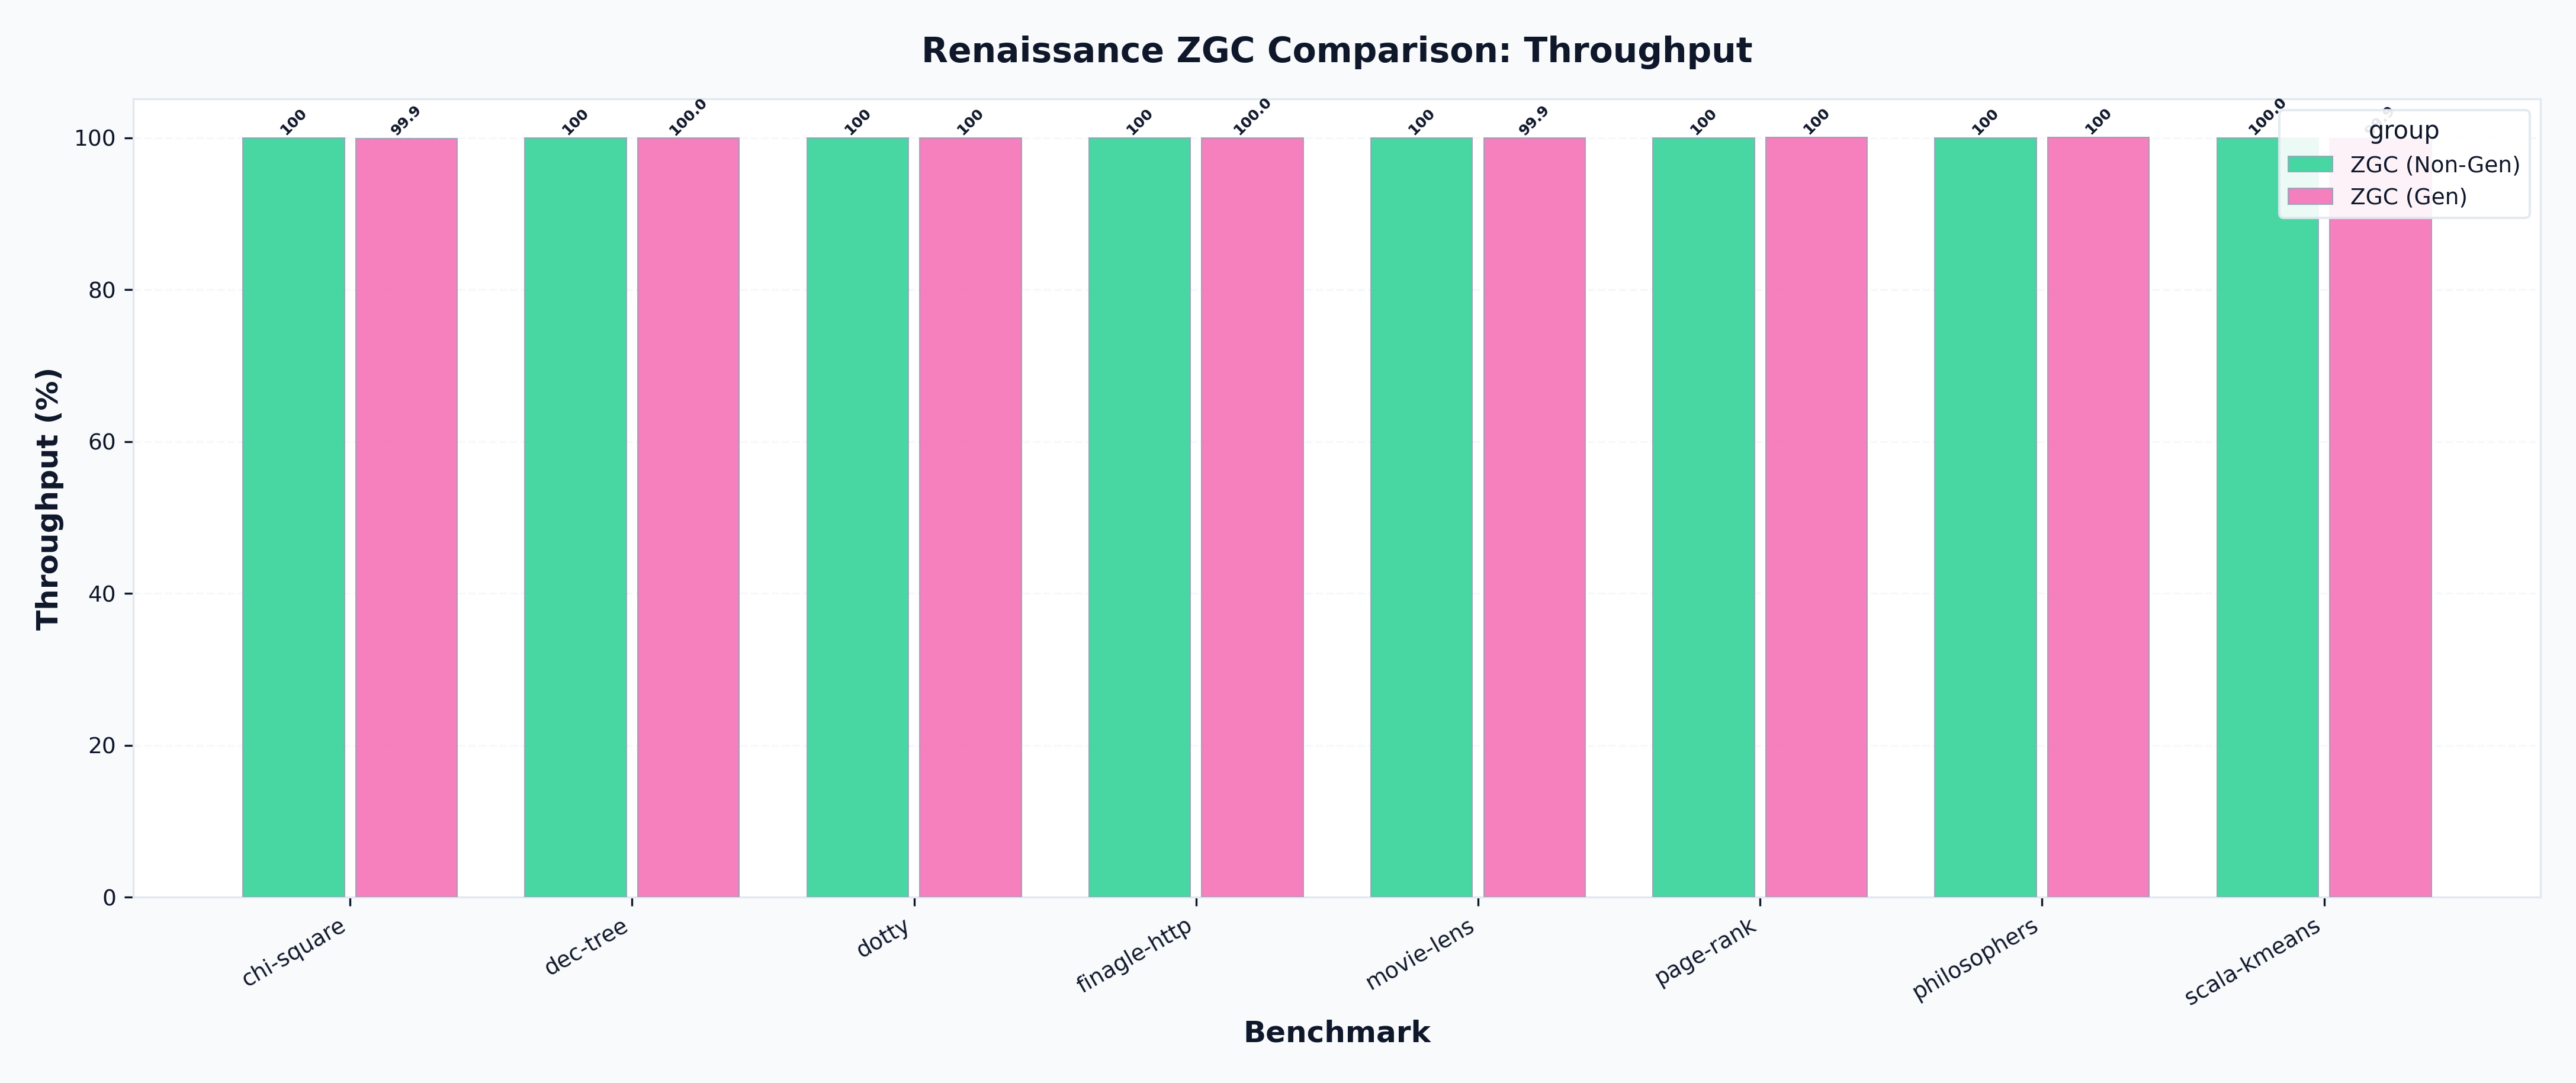
\includegraphics[width=\linewidth]{graphs/renaissance/zgc_comparison/renaissance_zgc_comparison_throughput_zgc.png}
\caption{Throughput}
\end{subfigure} \\

\begin{subfigure}{0.45\textwidth}
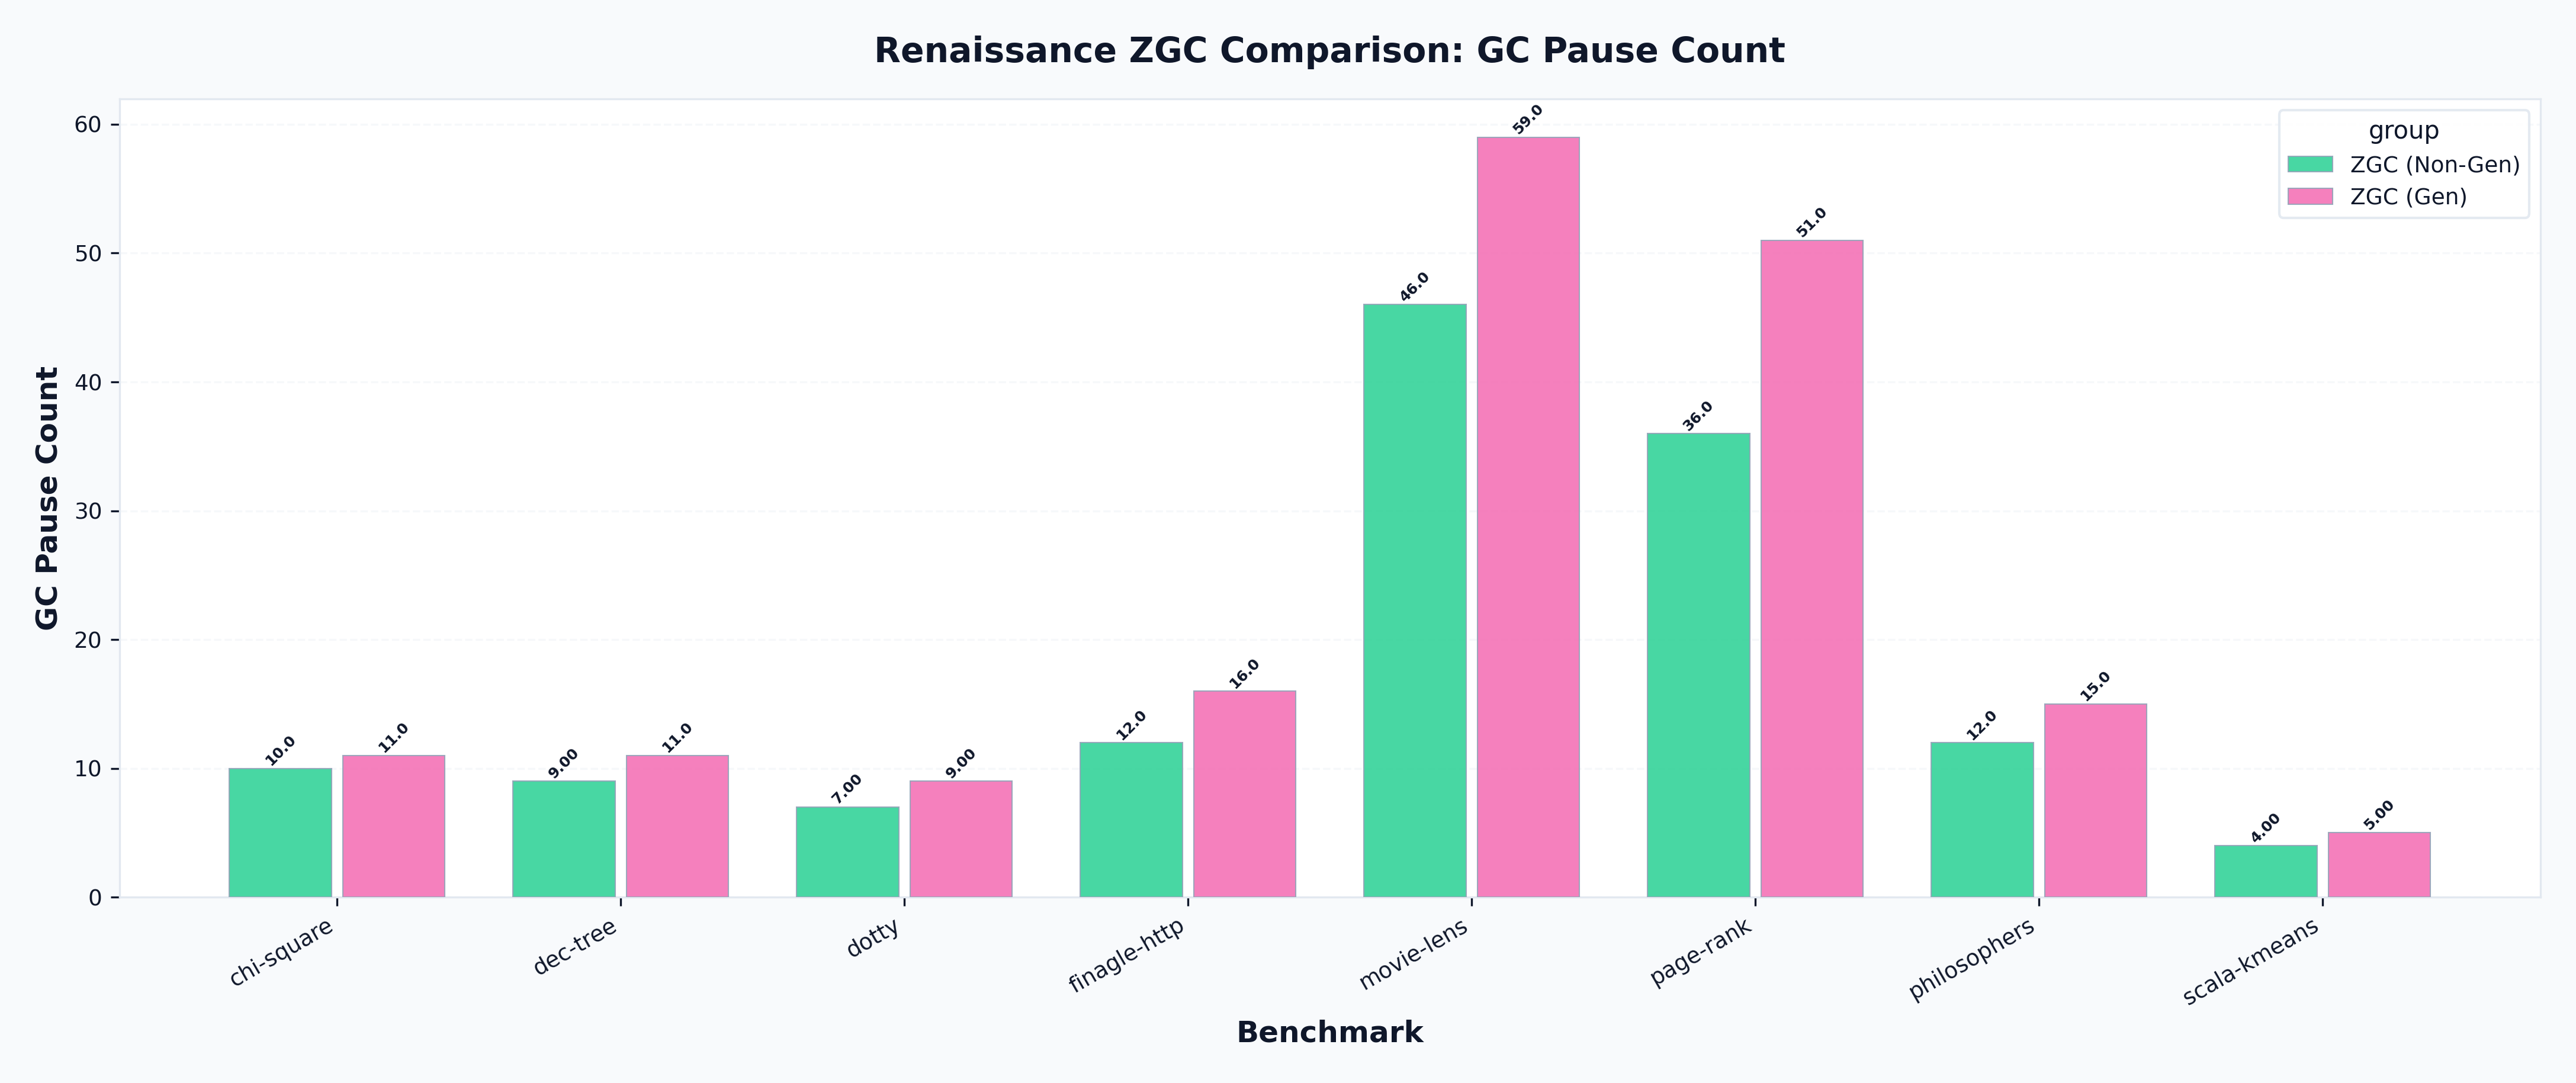
\includegraphics[width=\linewidth]{graphs/renaissance/zgc_comparison/renaissance_zgc_comparison_pauseCount_zgc.png}
\caption{Pause Count}
\end{subfigure} &
\begin{subfigure}{0.45\textwidth}
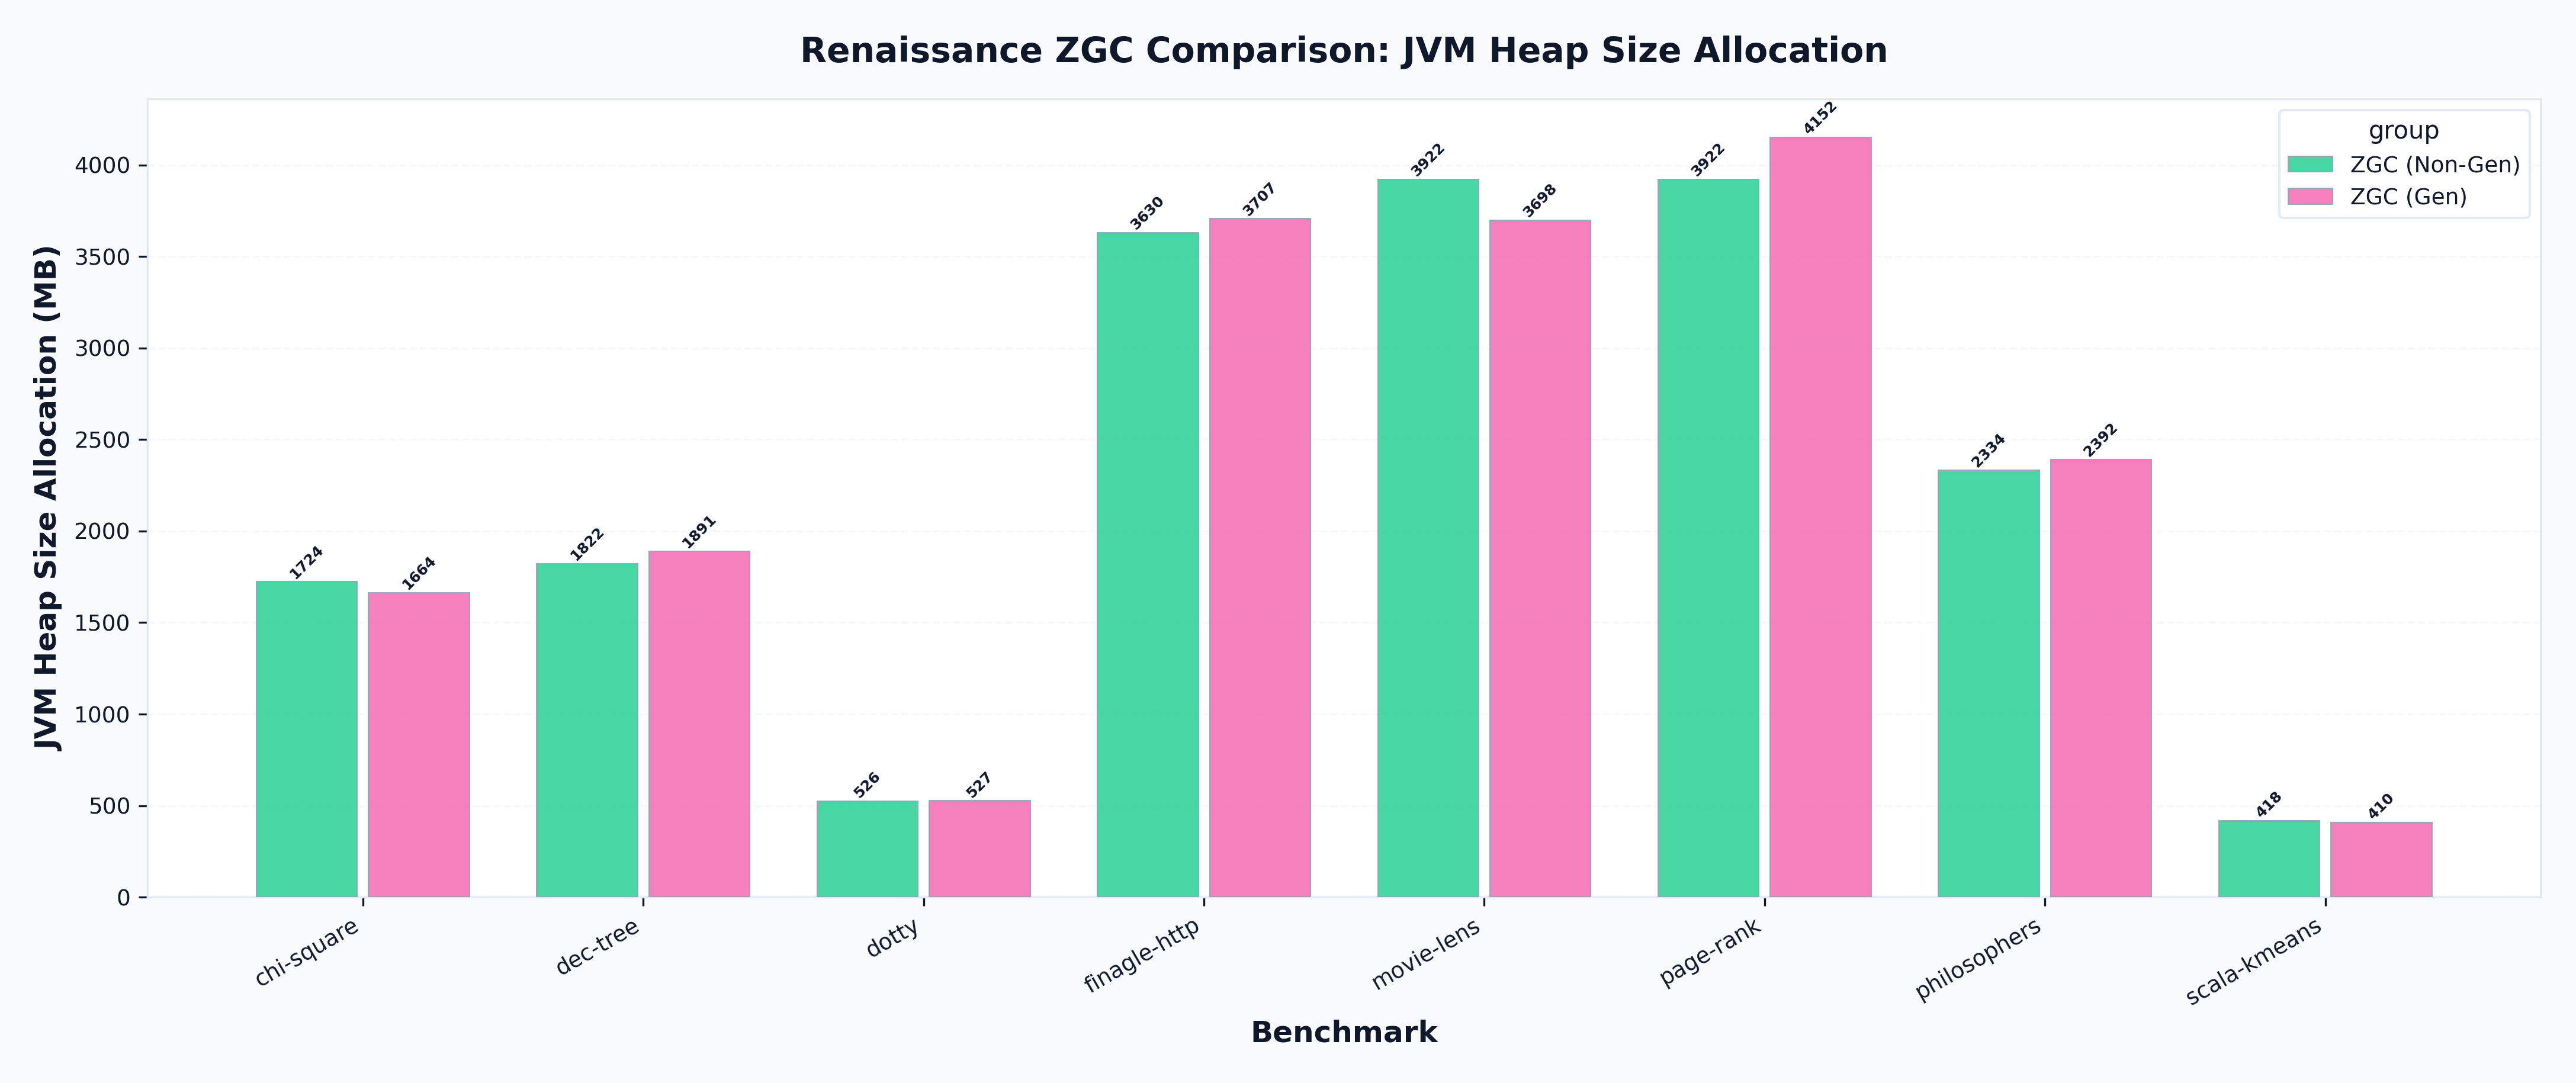
\includegraphics[width=\linewidth]{graphs/renaissance/zgc_comparison/renaissance_zgc_comparison_totalHeapAllocMax_zgc.png}
\caption{Total Heap Alloc Max}
\end{subfigure} \\

\begin{subfigure}{0.45\textwidth}
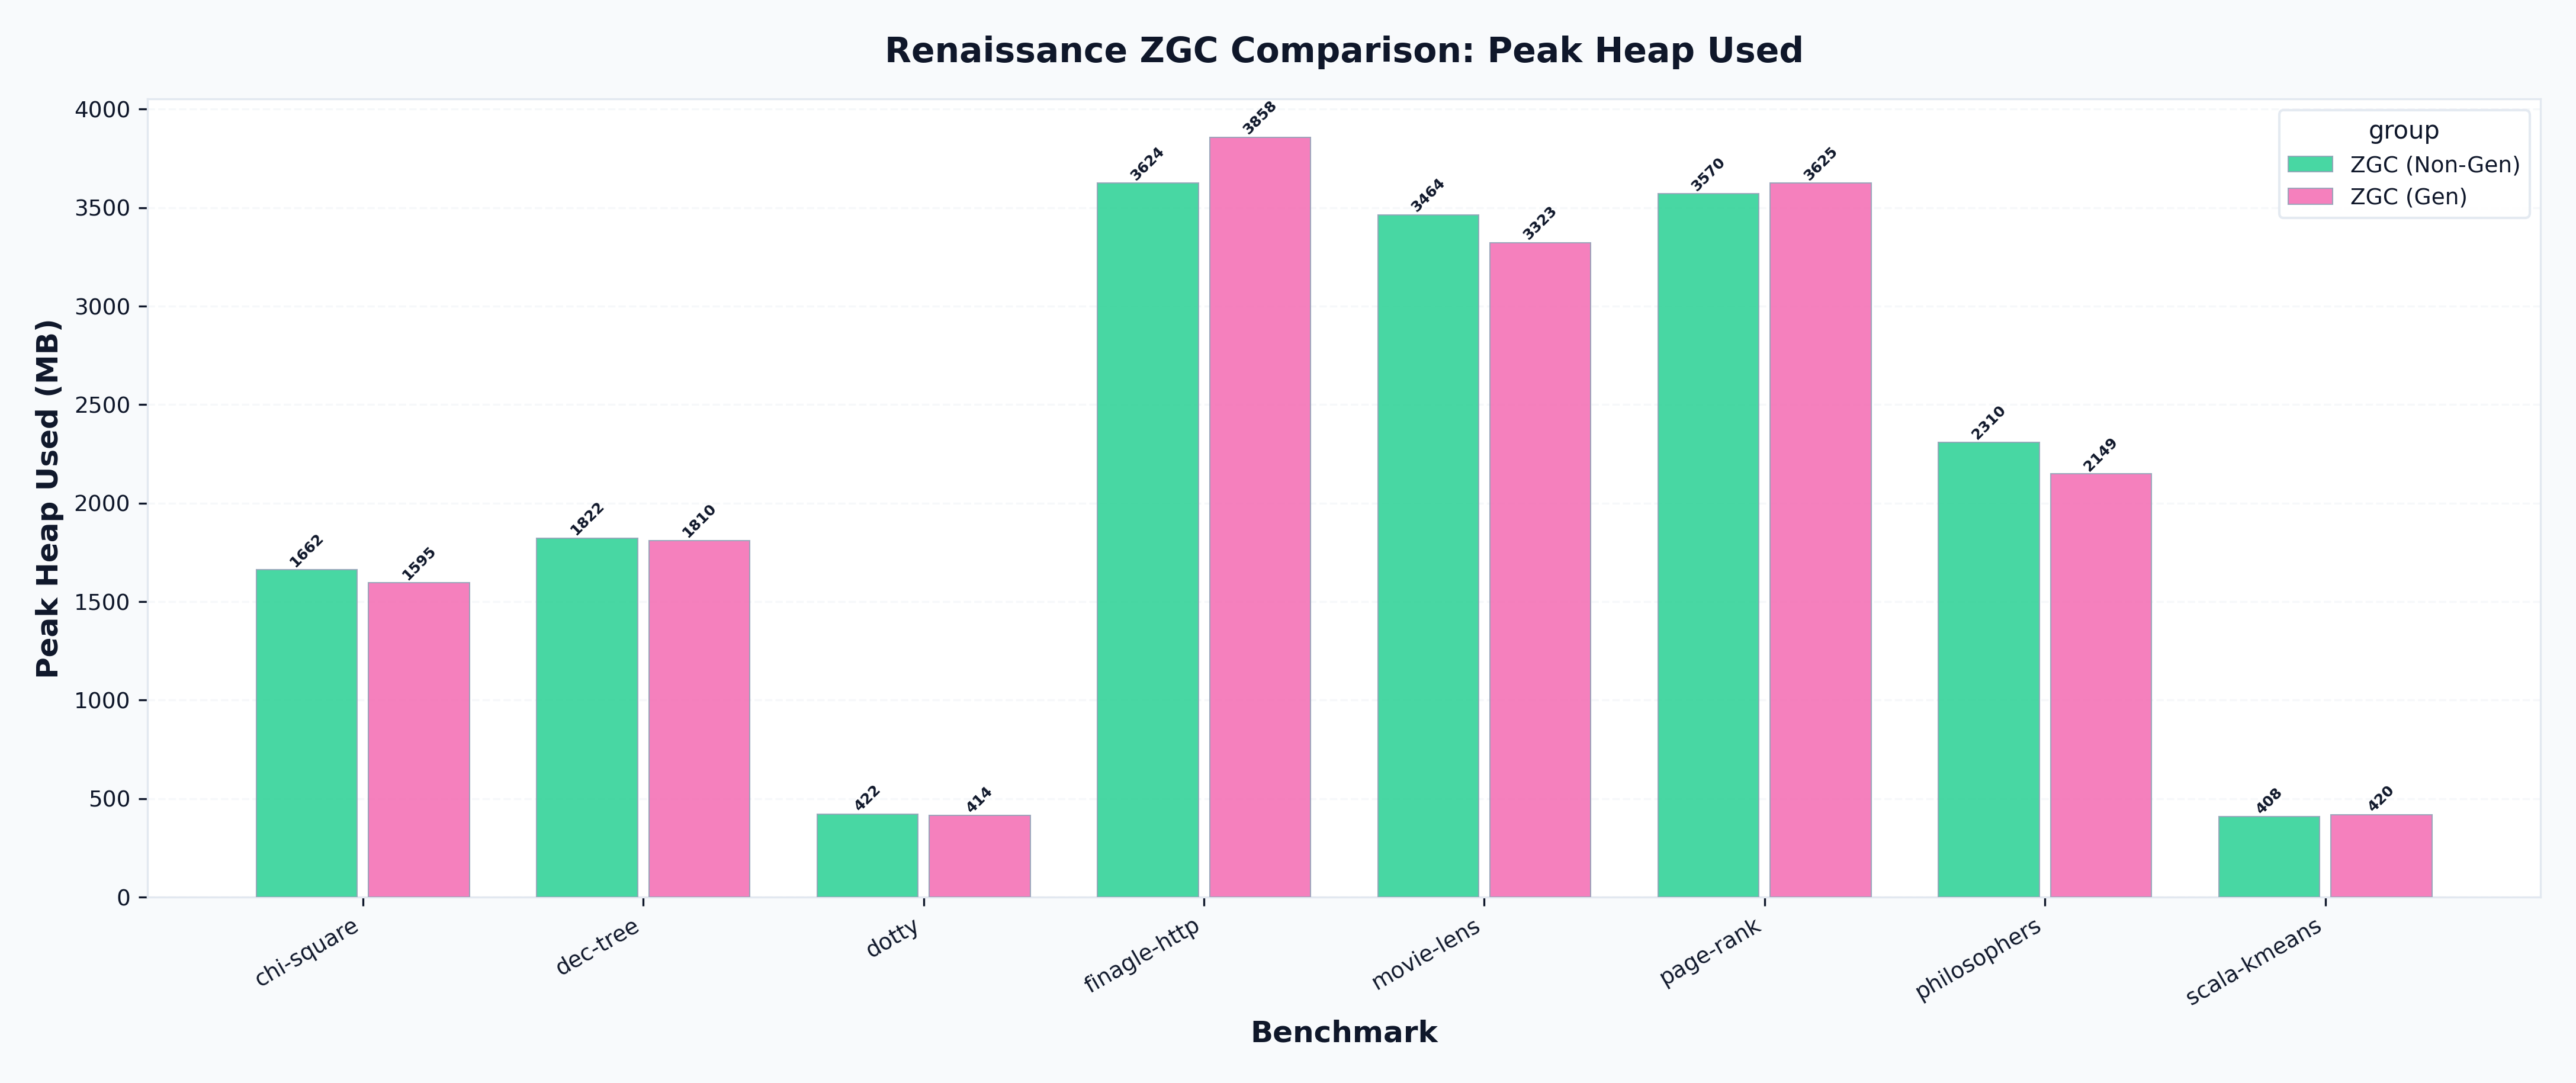
\includegraphics[width=\linewidth]{graphs/renaissance/zgc_comparison/renaissance_zgc_comparison_totalHeapUsedMax_zgc.png}
\caption{Total Heap Used Max}
\end{subfigure} &
\begin{subfigure}{0.45\textwidth}
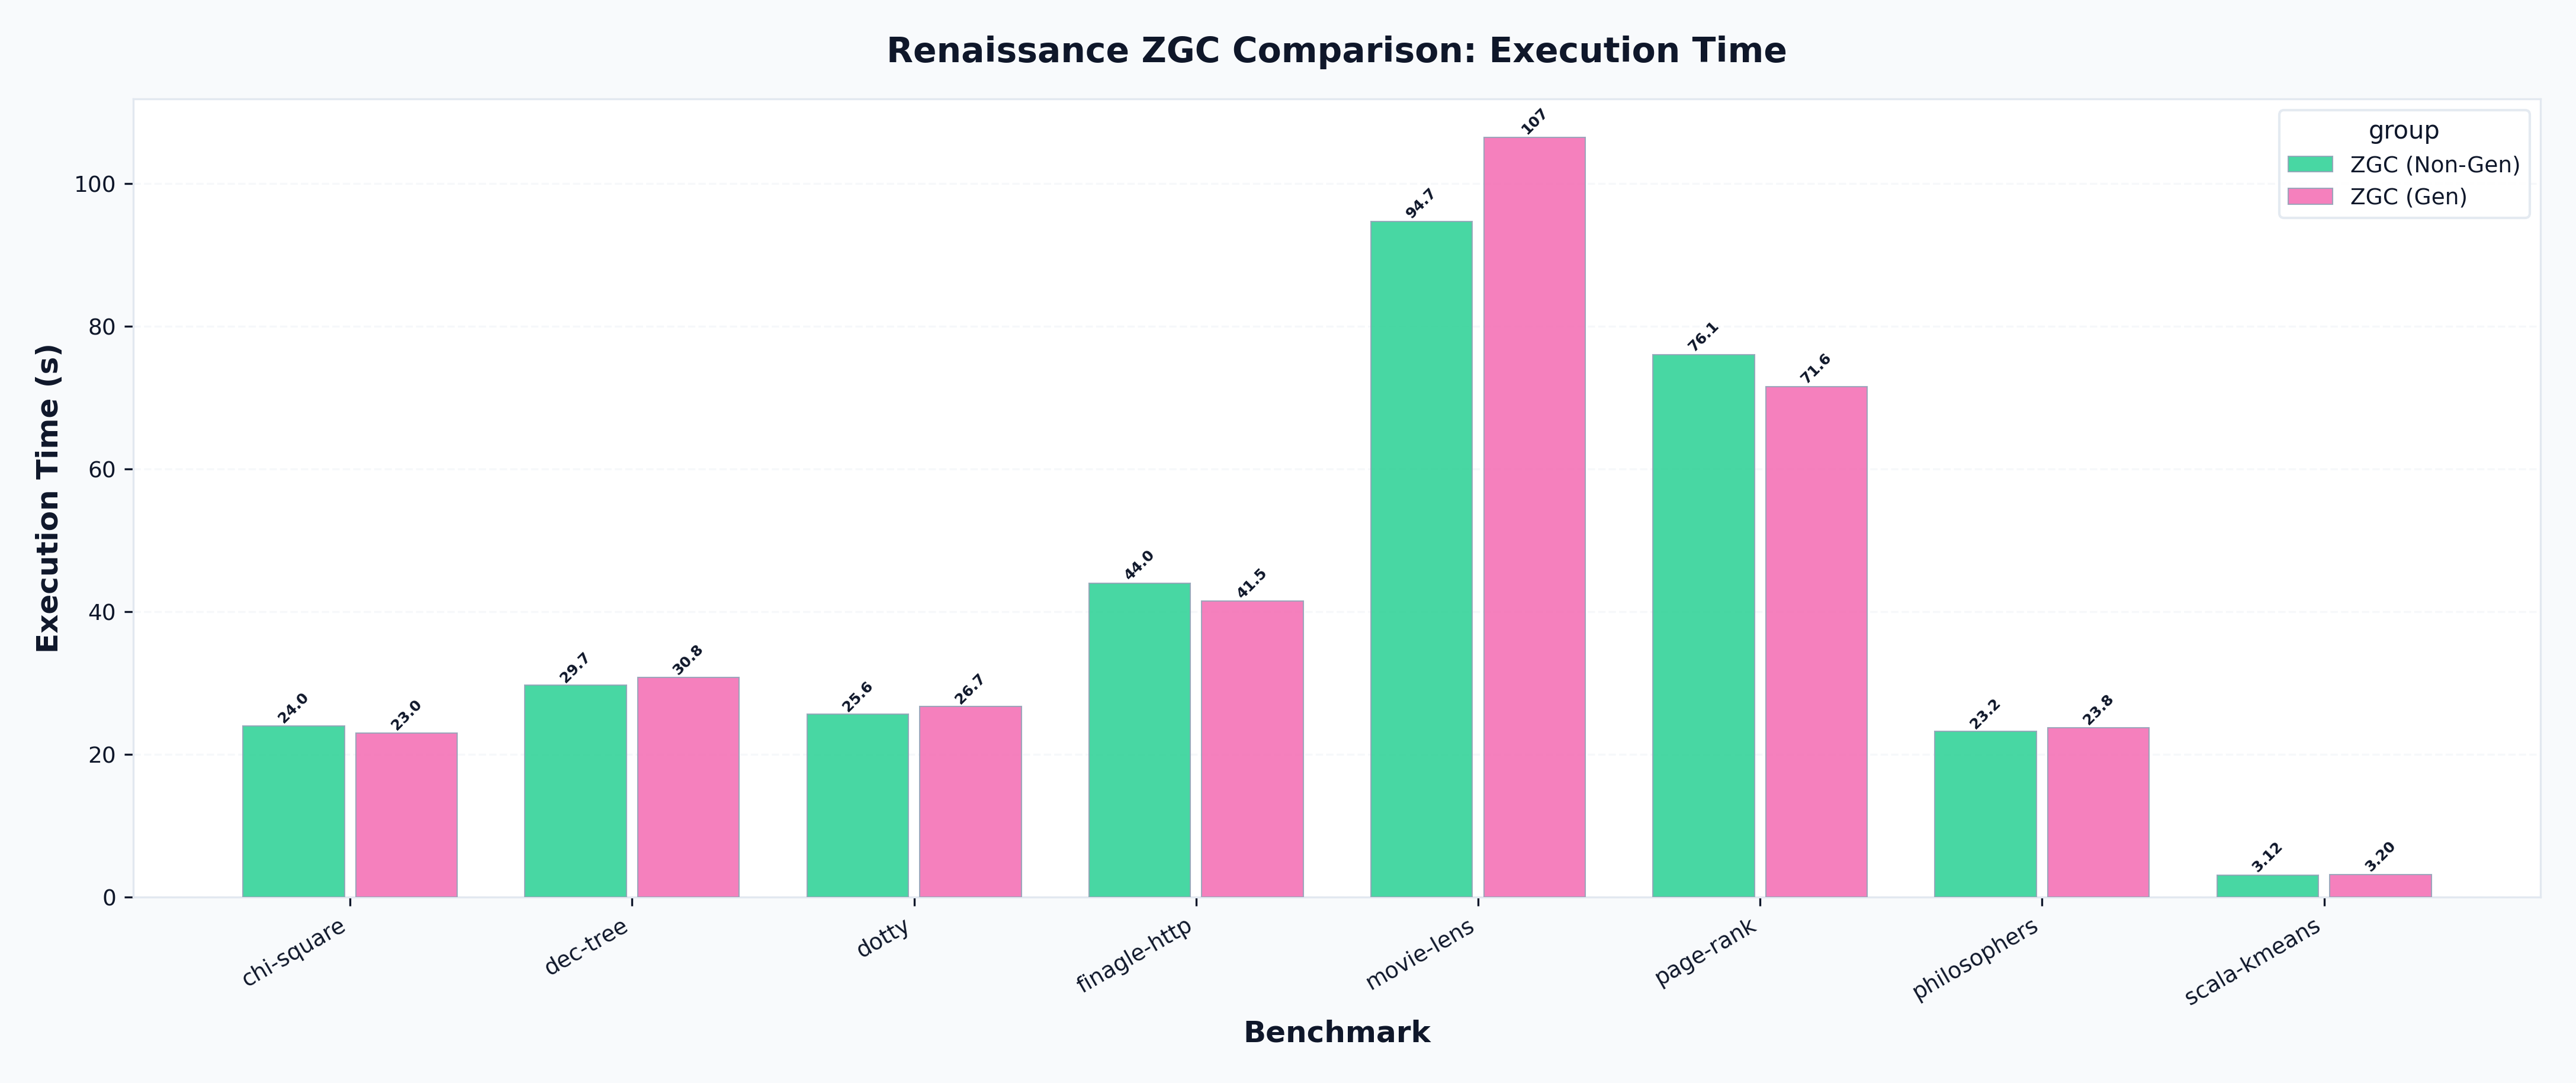
\includegraphics[width=\linewidth]{graphs/renaissance/zgc_comparison/renaissance_zgc_comparison_wallTimeSec_zgc.png}
\caption{Wall Time (sec)}
\end{subfigure} \\

\end{tabular}

\caption{ZGC Comparison Across Renaissance Benchmarks Using Different Metrics}
\label{fig:renaissance_zgc_comparison}
\end{figure}

% heap vary %

\subsubsection{Heap Size Variation}
To evaluate the resilience of each garbage collector under memory pressure, we executed benchmarks with maximum heap sizes dynamically restricted by up to 50\% of the recommended allocation. Figure \ref{fig:chi_heap_vary}, Figure \ref{fig:movie_lens_heap_vary}, and Figure \ref{fig:page_rank_heap_vary} detail these adjustments. Across most benchmarks, generously sizing the heap proportionally reduces GC pause frequencies and improves throughput by roughly 15-20\%. Notably, ZGC and Shenandoah maintain their characteristically consistent average pause times of below 2ms even when operating under heavily constrained configurations. In contrast, G1GC exhibits noticeable degradation, with average pause times nearly doubling when heap limits are strictly enforced.

\begin{figure}[h]
\centering

\begin{tabular}{cc}

\begin{subfigure}{0.45\textwidth}
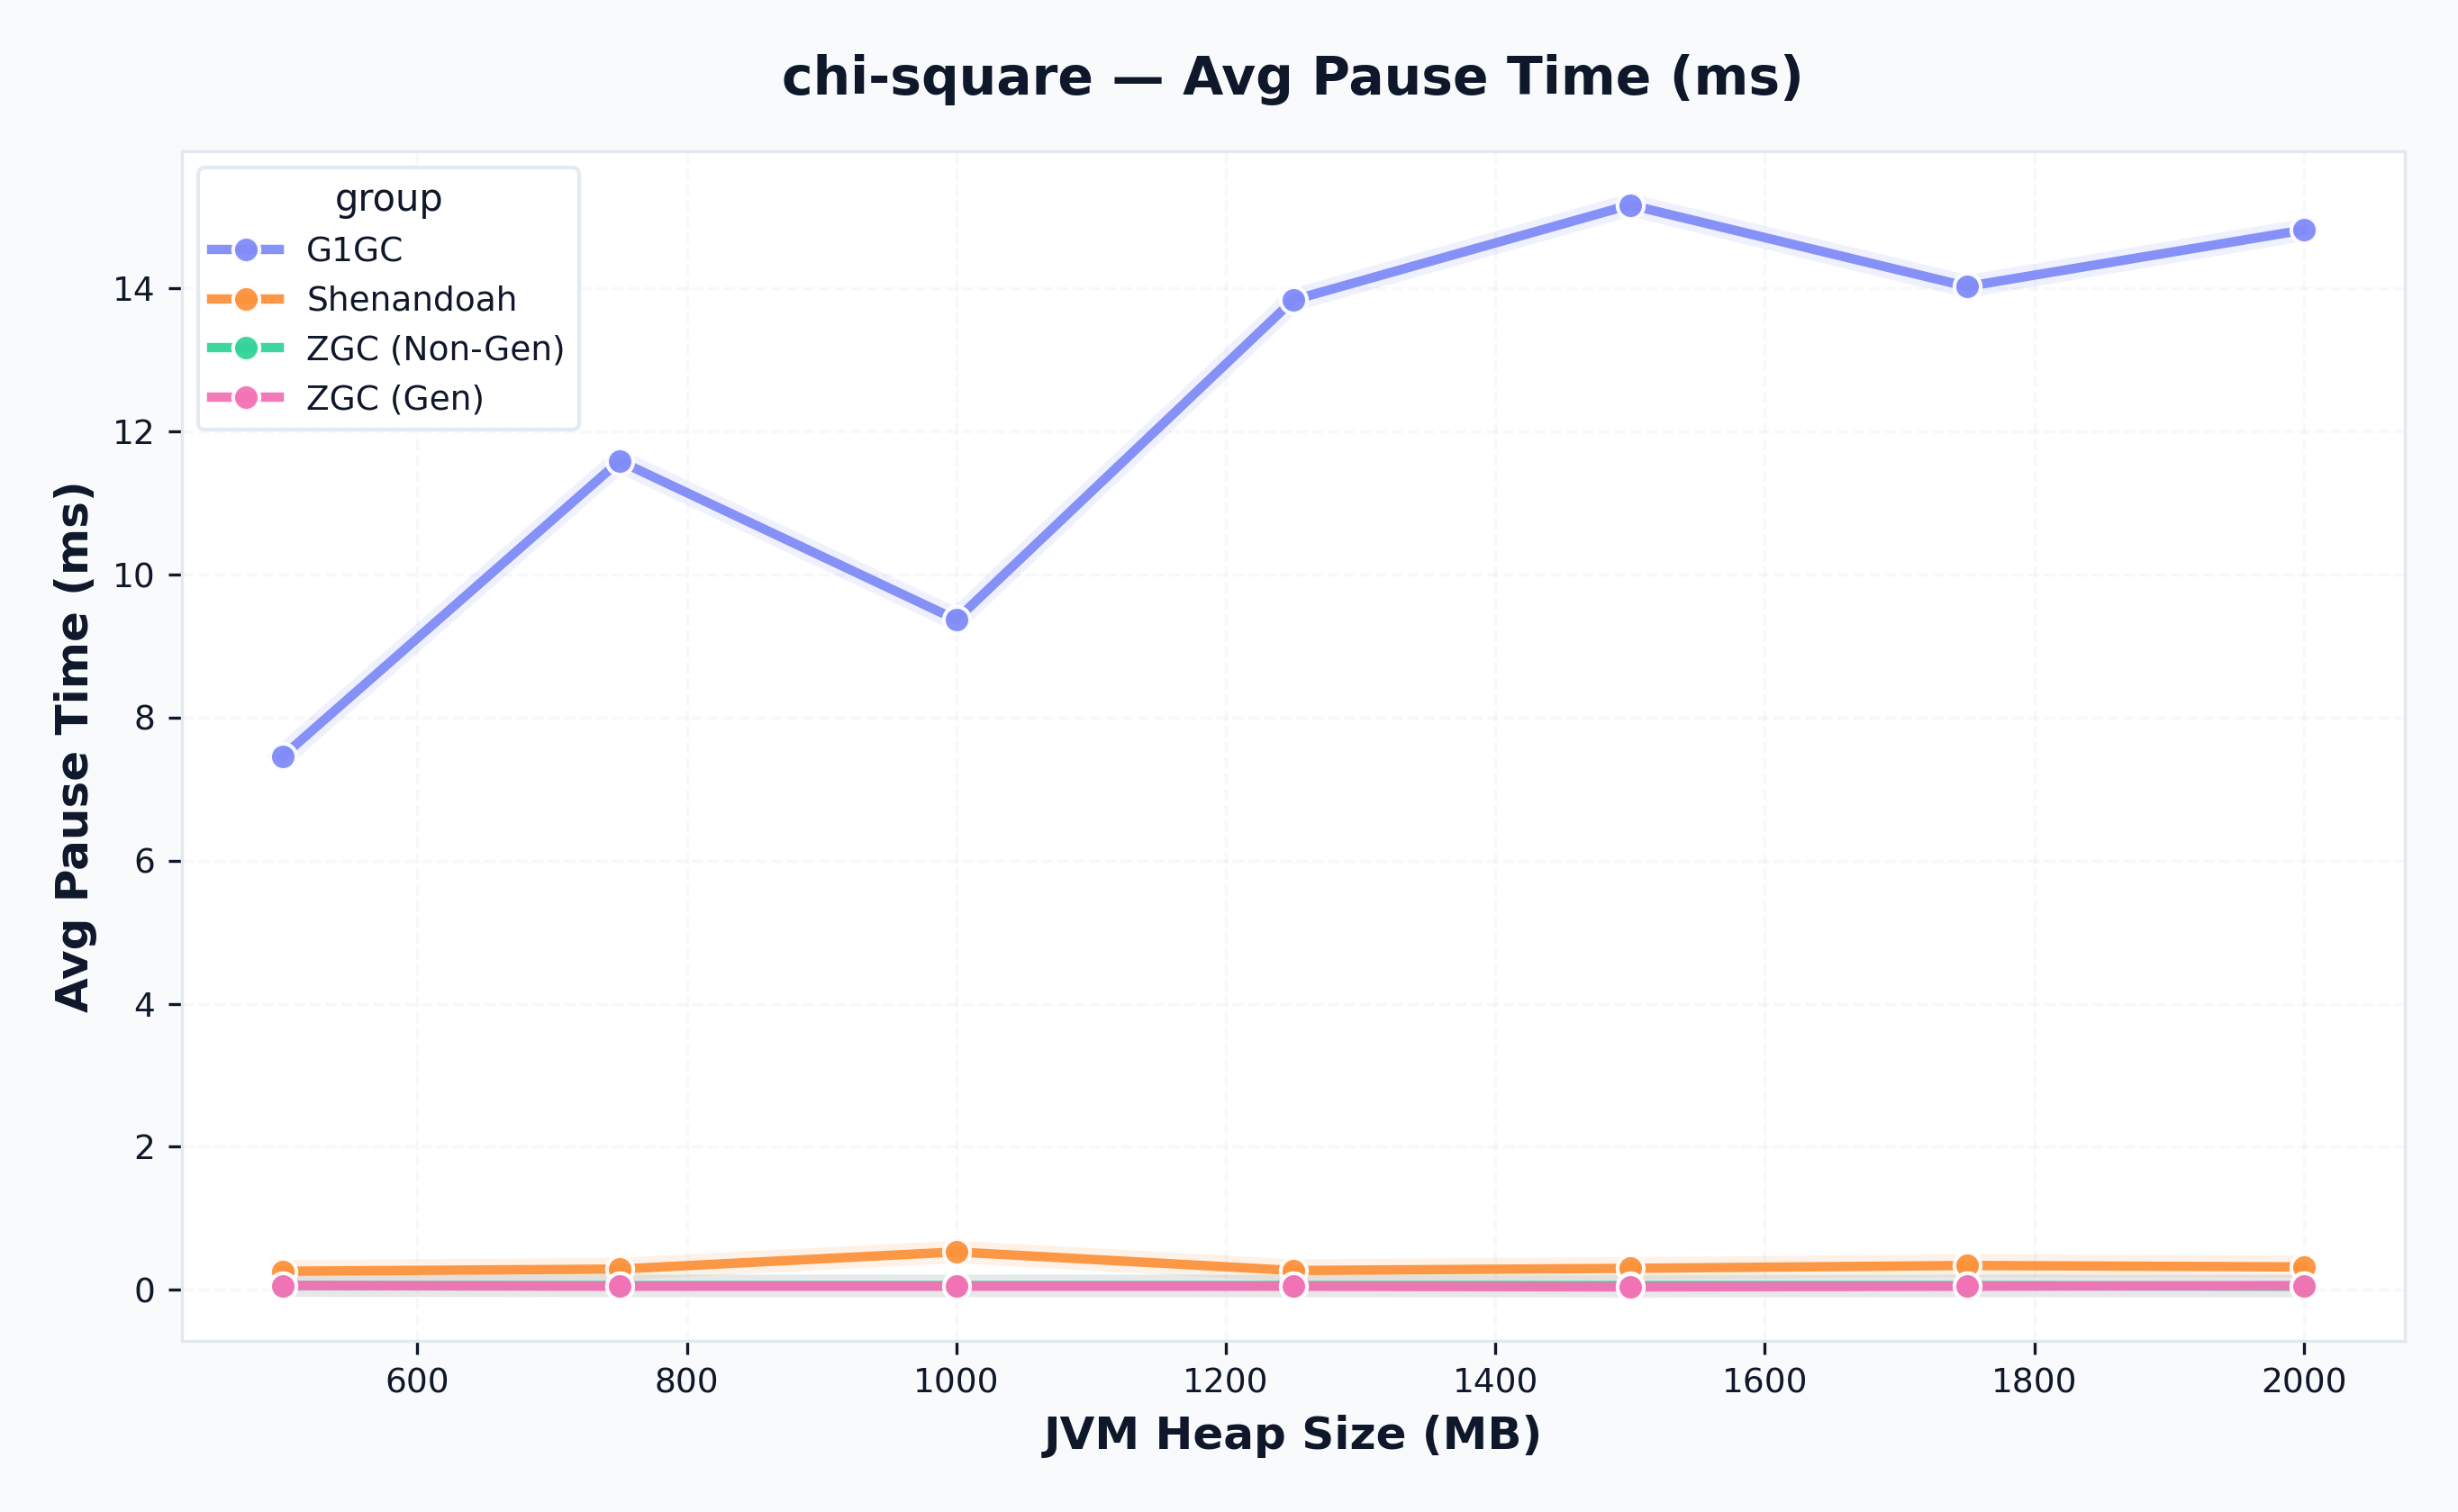
\includegraphics[width=\linewidth]{graphs/heap_vary/chi-square/heap_vary_avgPause.png}
\caption{Average Pause}
\end{subfigure} &
\begin{subfigure}{0.45\textwidth}
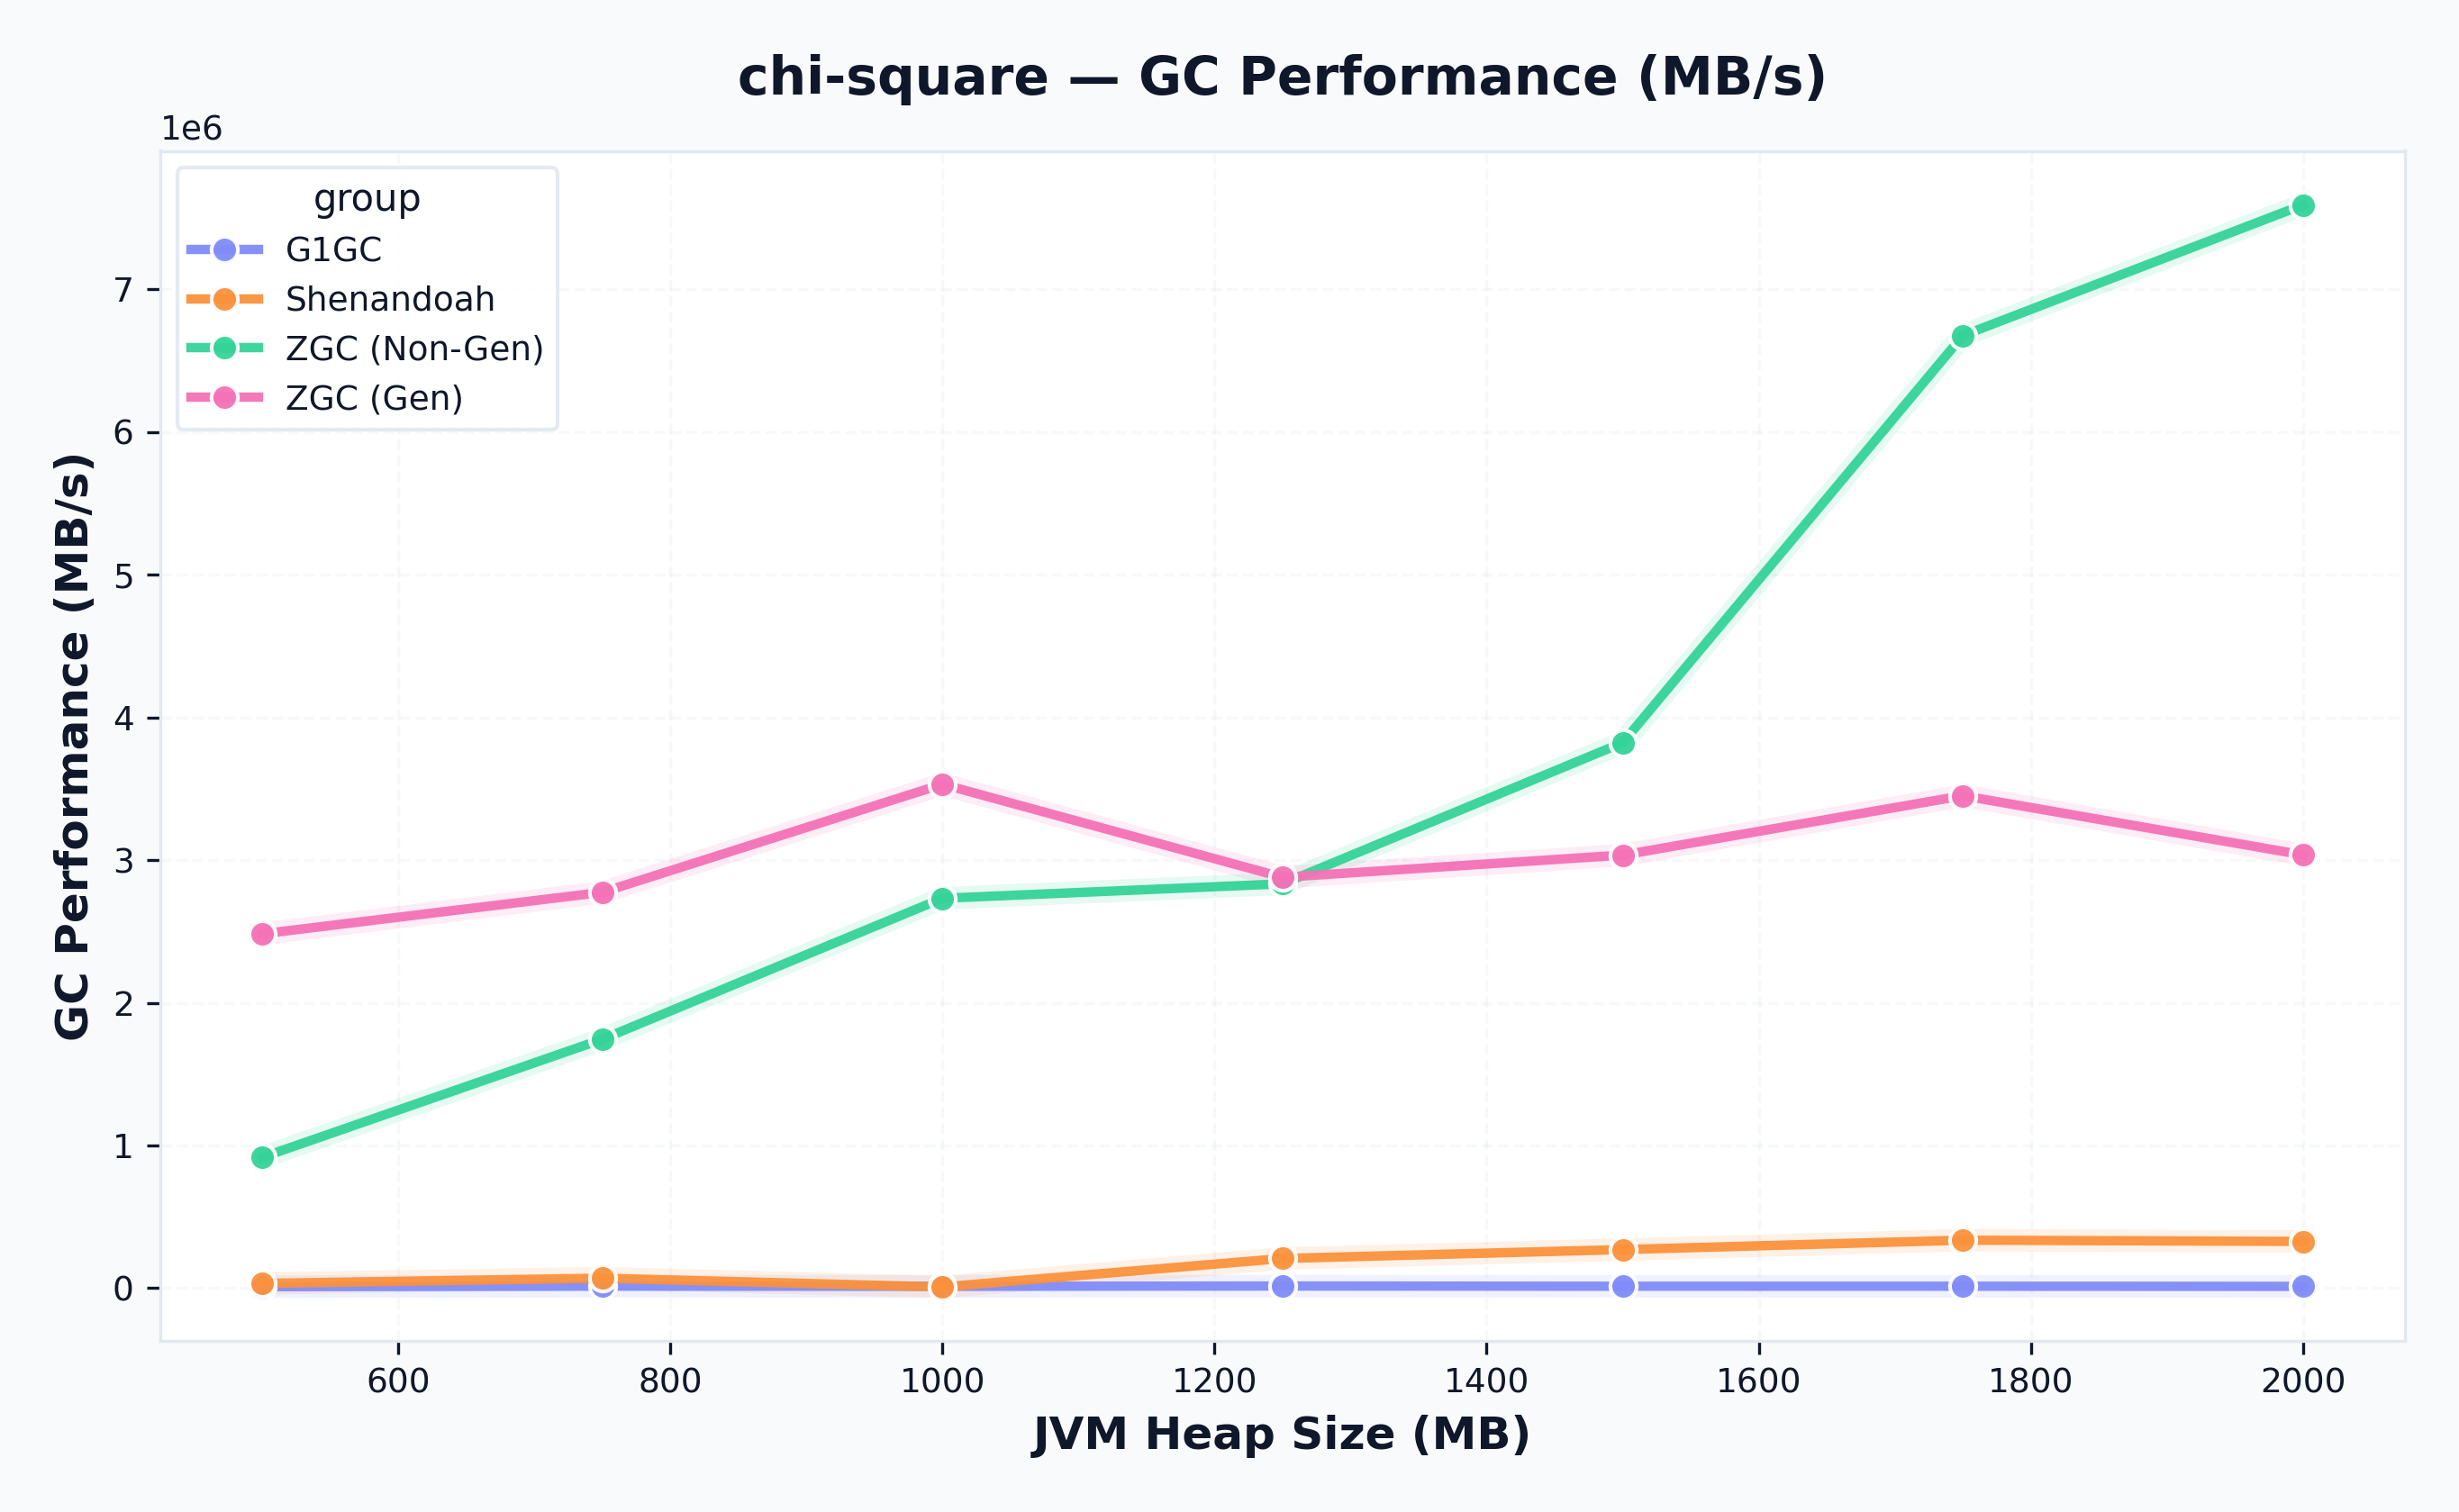
\includegraphics[width=\linewidth]{graphs/heap_vary/chi-square/heap_vary_gcPerformance.png}
\caption{GC Performance}
\end{subfigure} \\

\begin{subfigure}{0.45\textwidth}
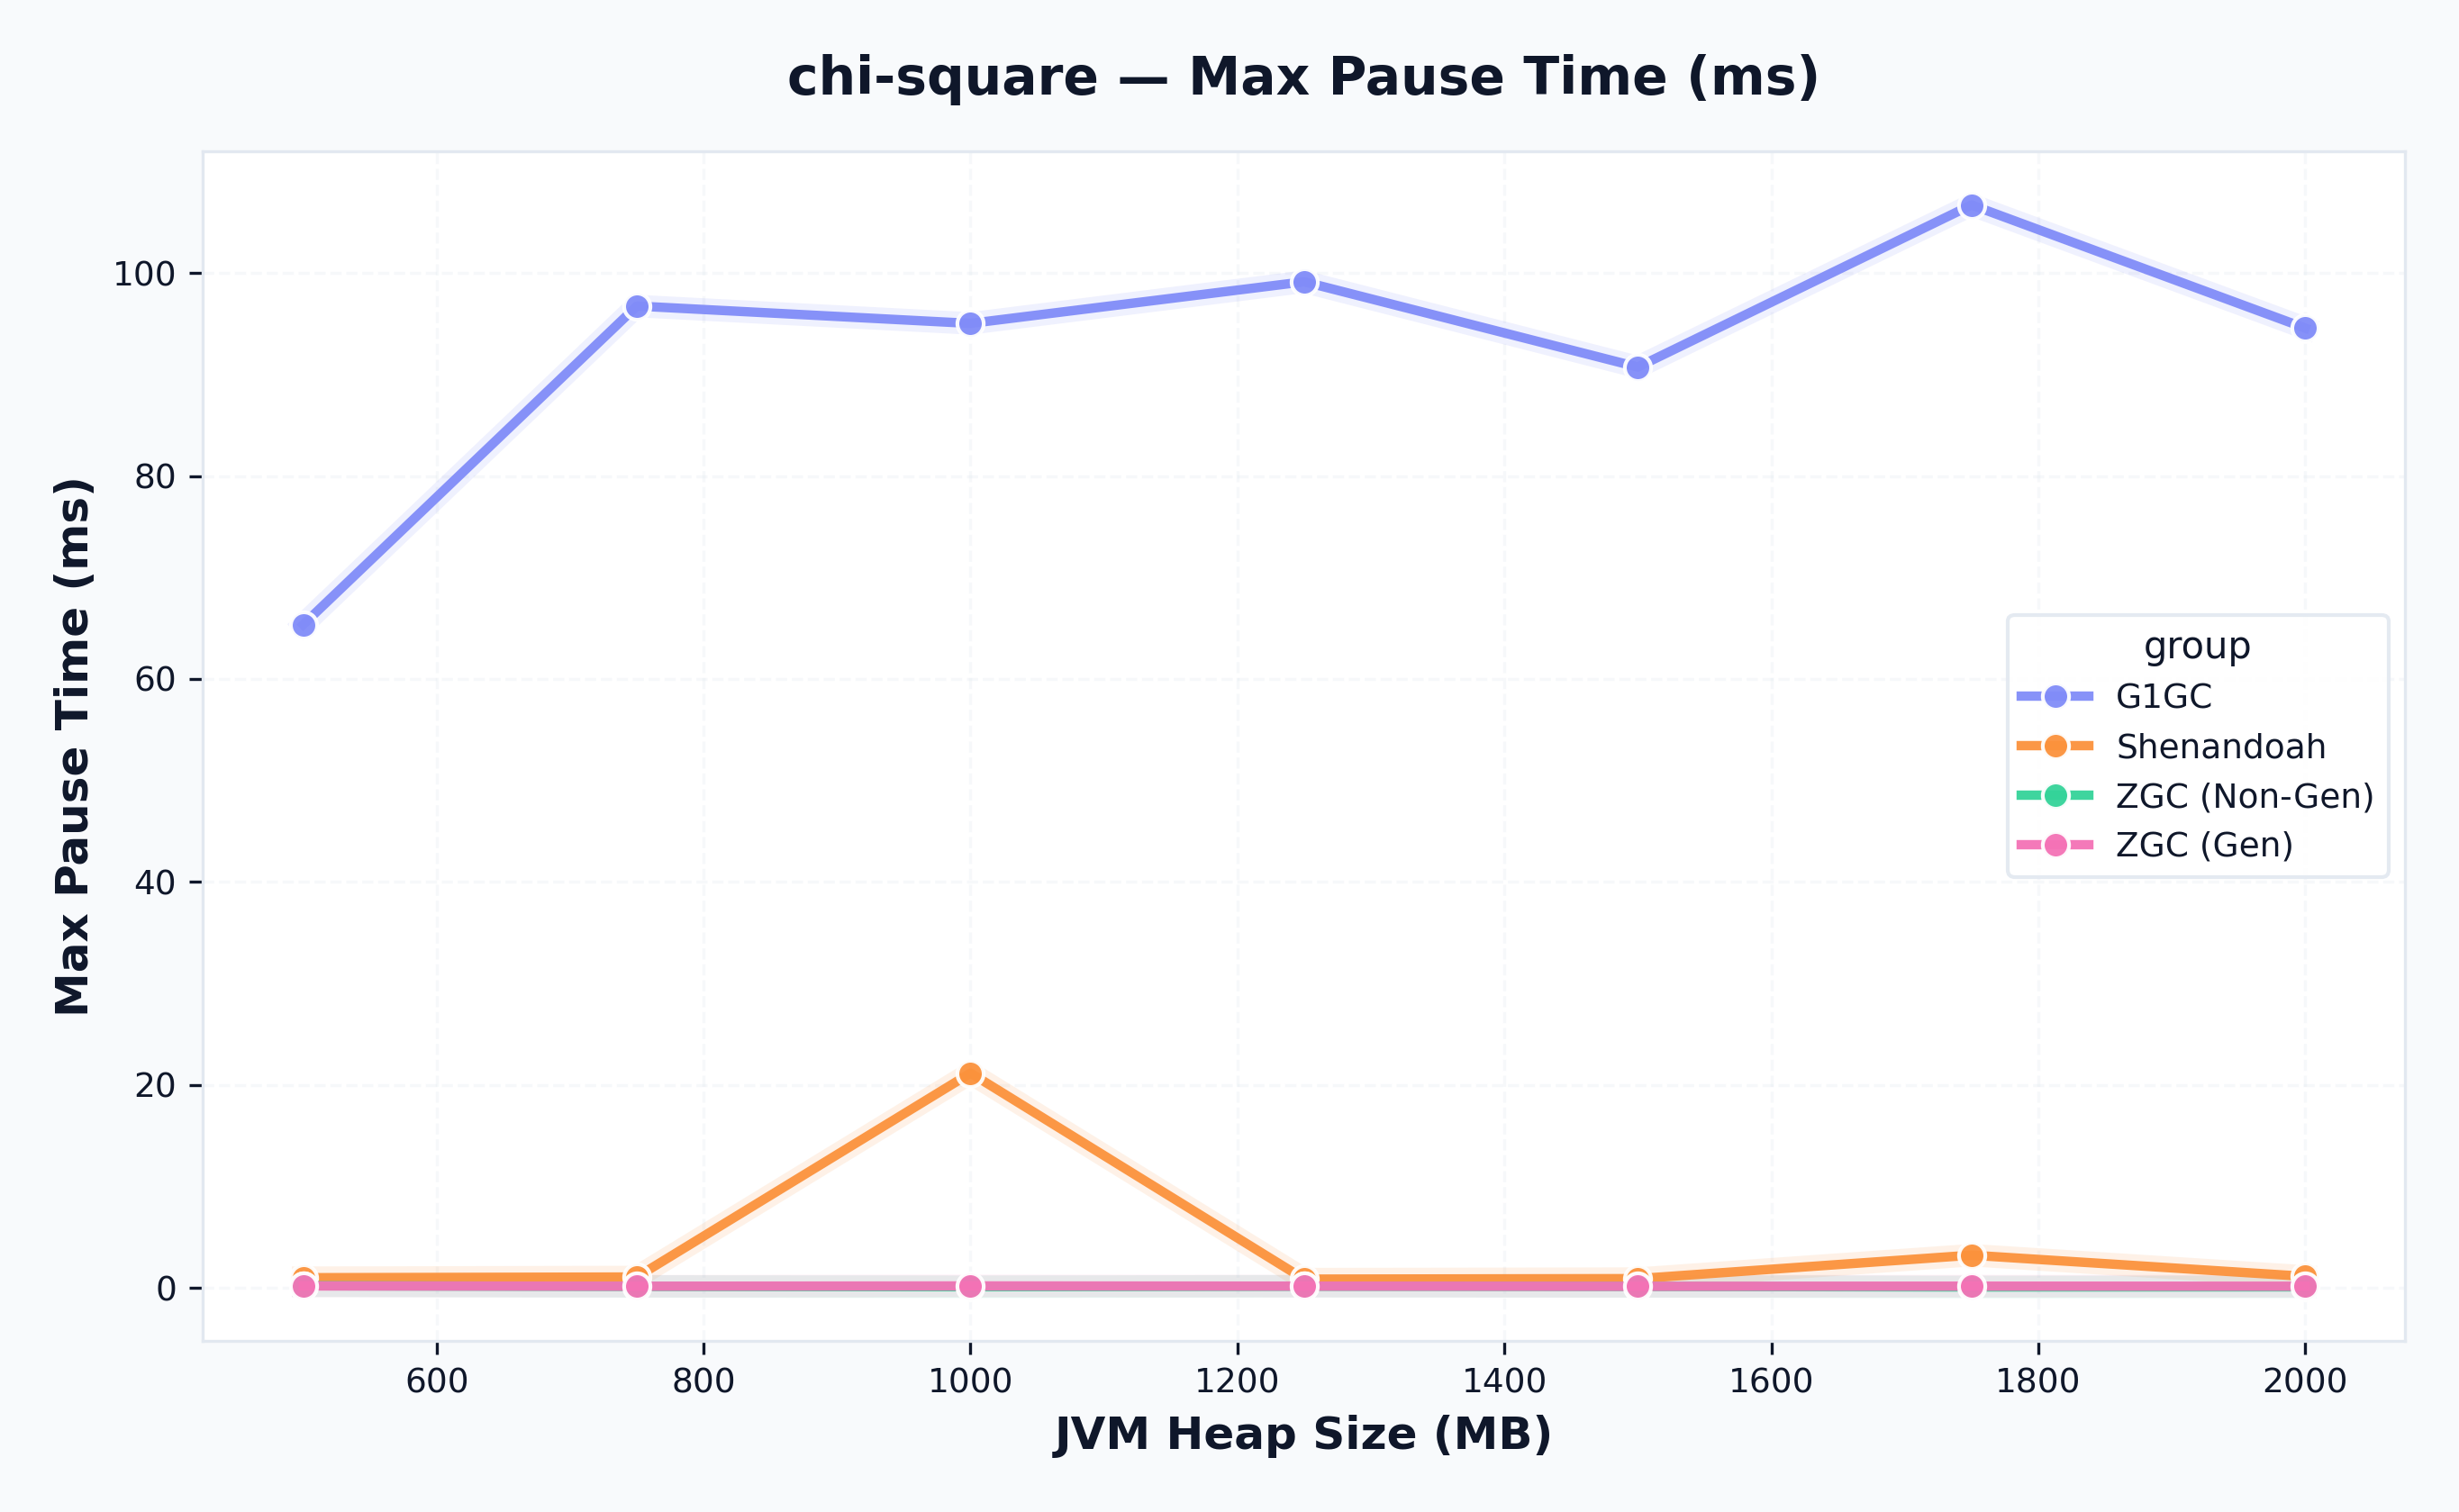
\includegraphics[width=\linewidth]{graphs/heap_vary/chi-square/heap_vary_maxPause.png}
\caption{Max Pause}
\end{subfigure} &
\begin{subfigure}{0.45\textwidth}
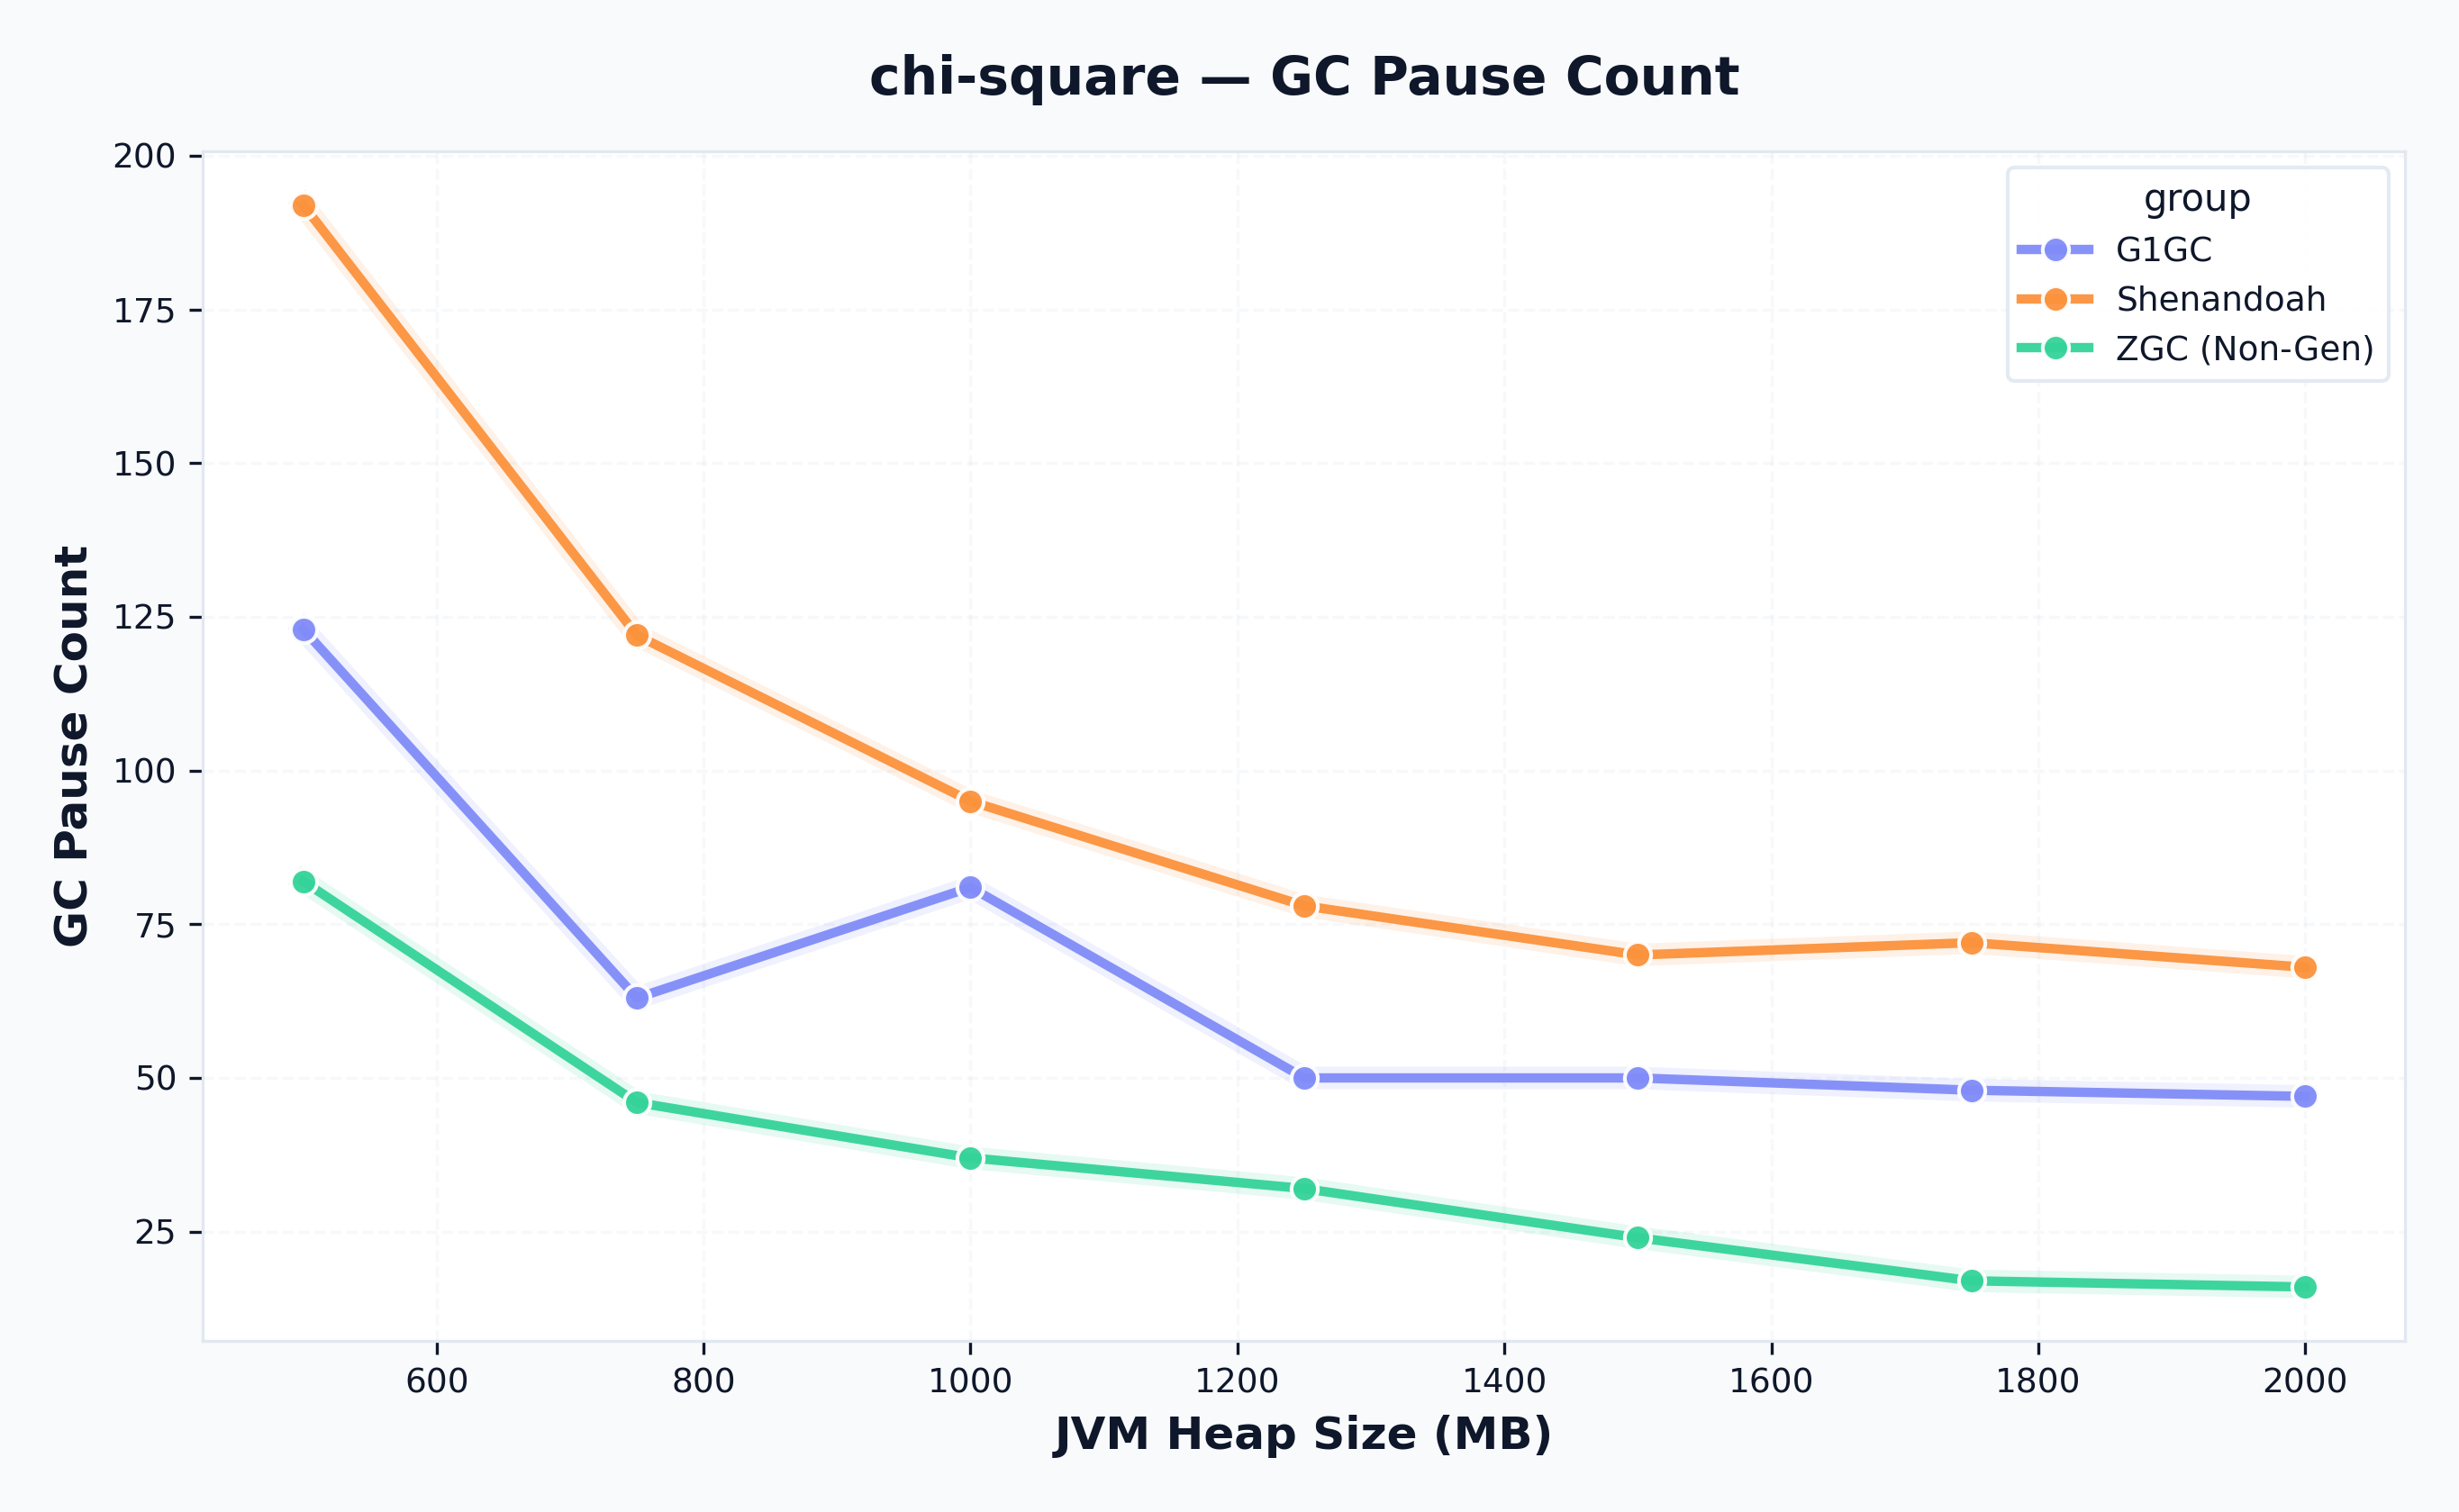
\includegraphics[width=\linewidth]{graphs/heap_vary/chi-square/heap_vary_pauseCount.png}
\caption{Pause Count}
\end{subfigure} \\

\begin{subfigure}{0.45\textwidth}
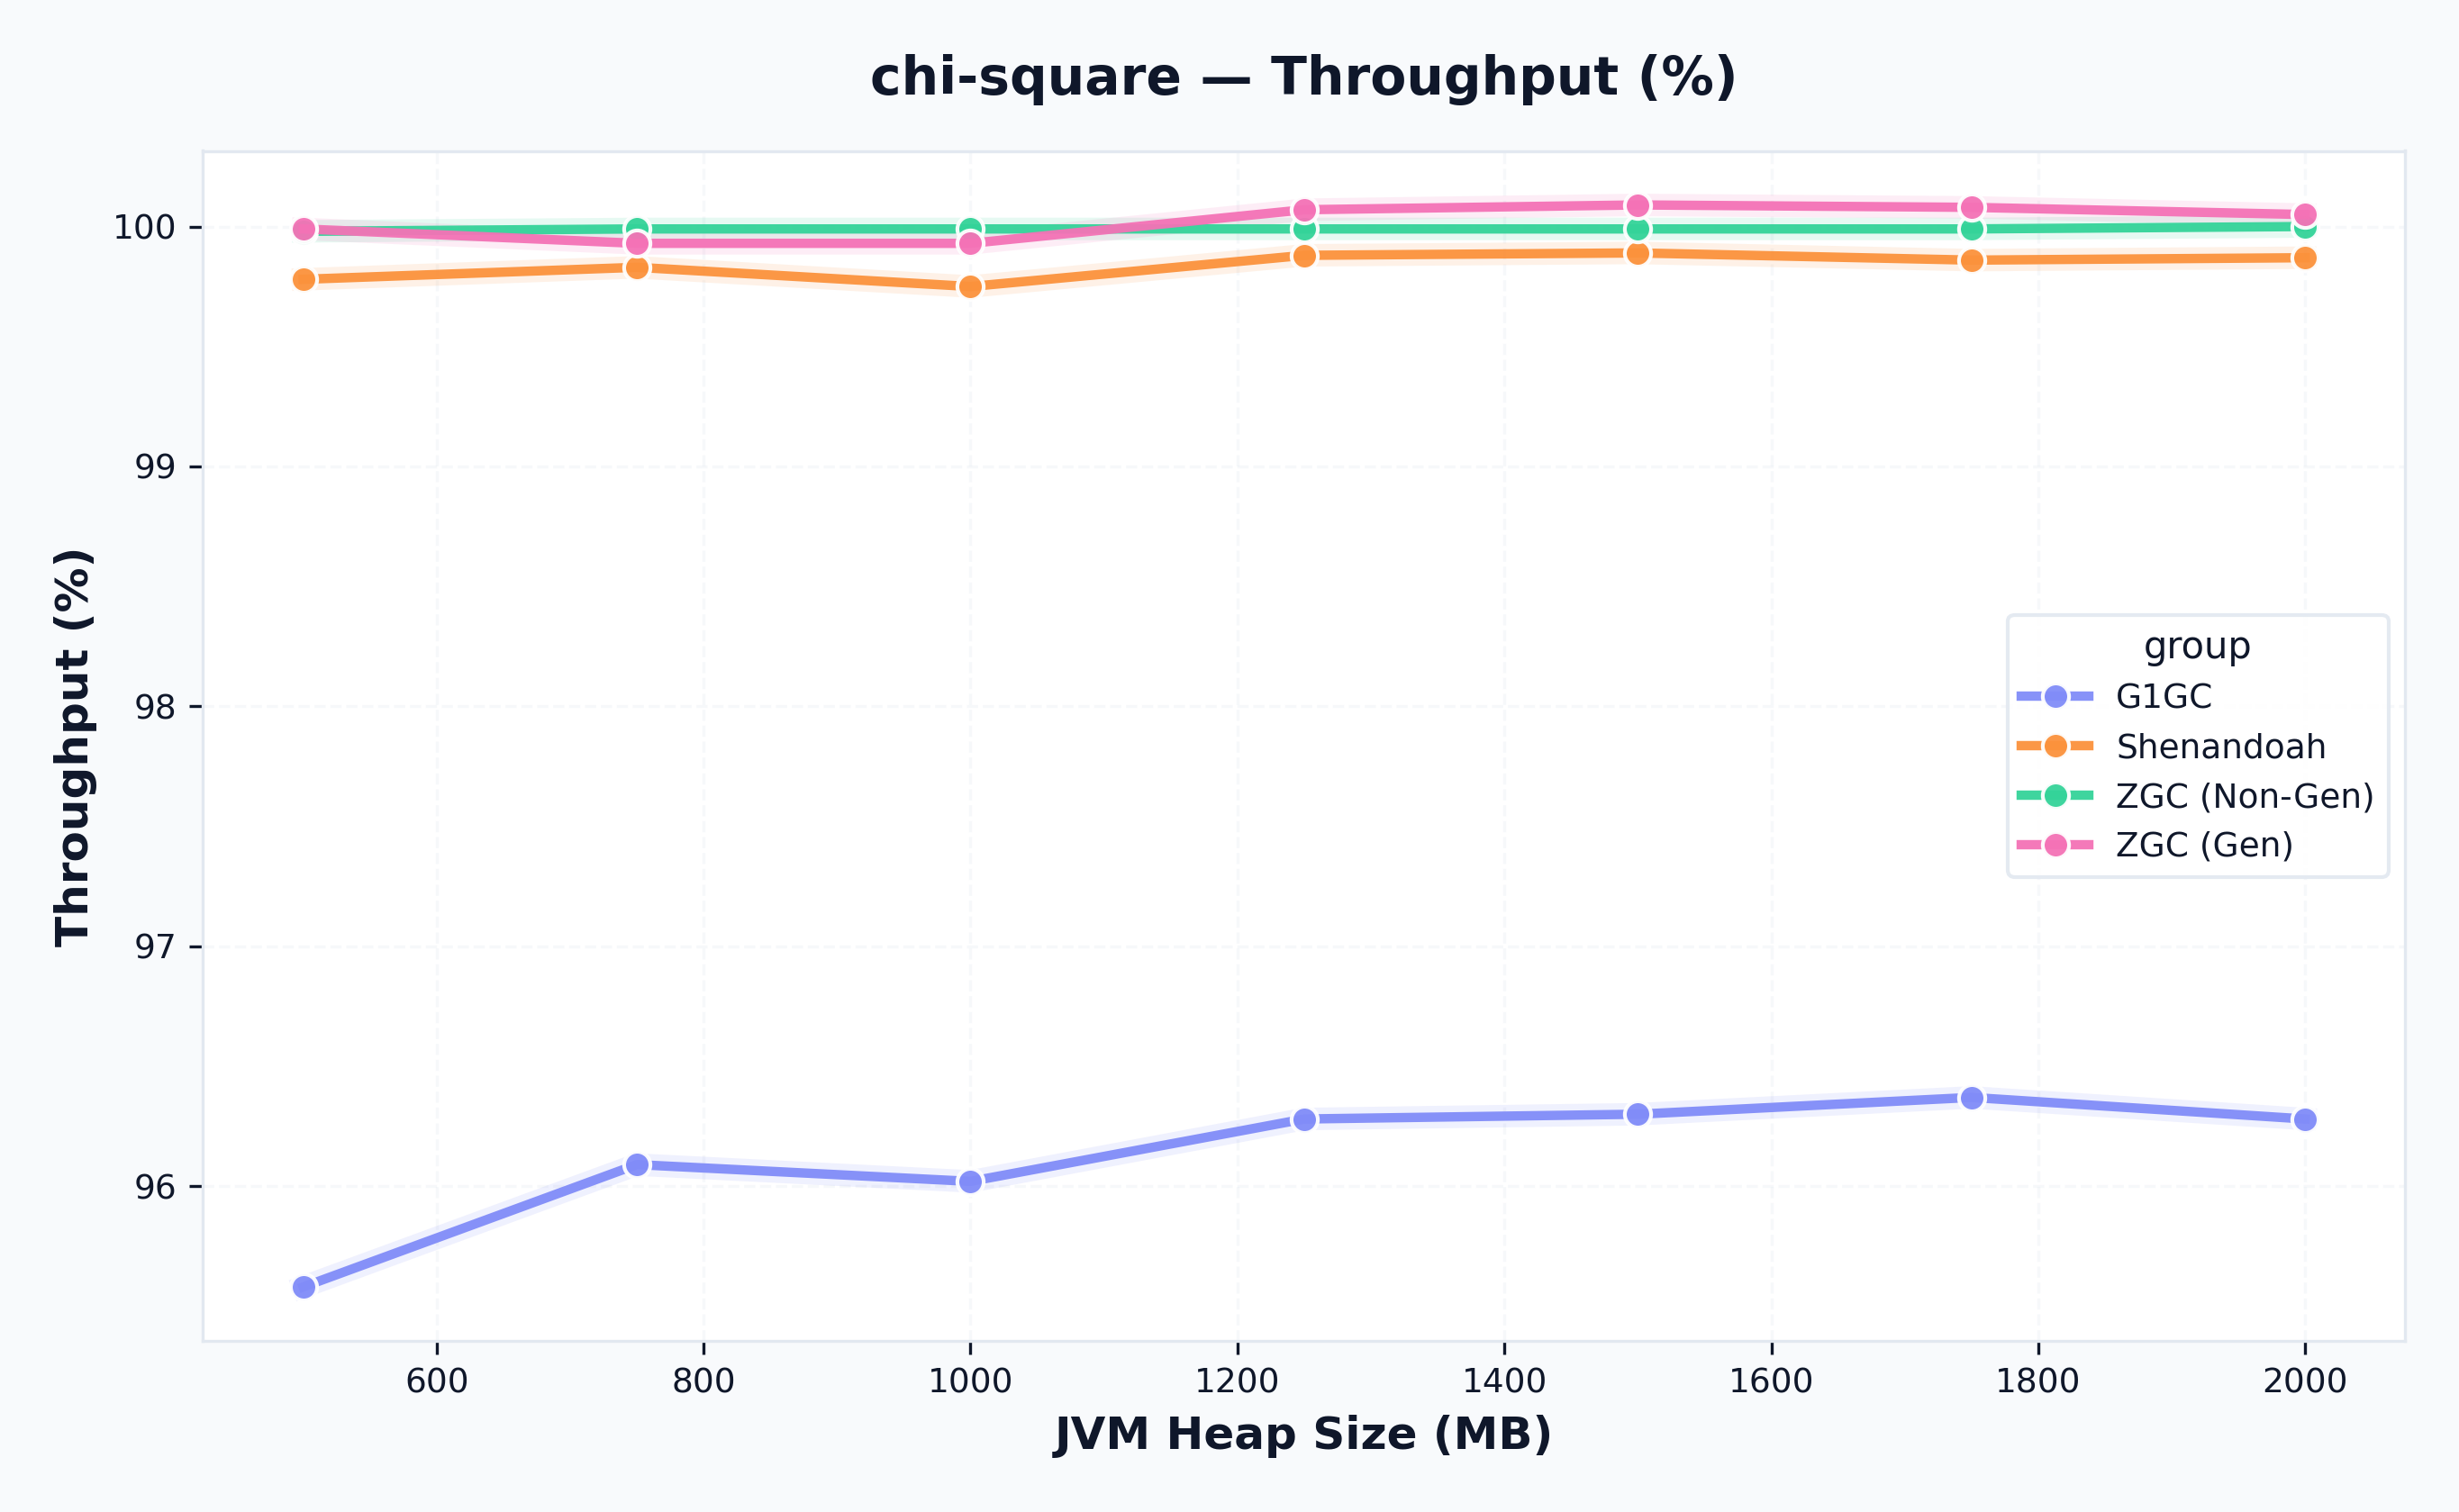
\includegraphics[width=\linewidth]{graphs/heap_vary/chi-square/heap_vary_throughput.png}
\caption{Throughput}
\end{subfigure} &
\begin{subfigure}{0.45\textwidth}
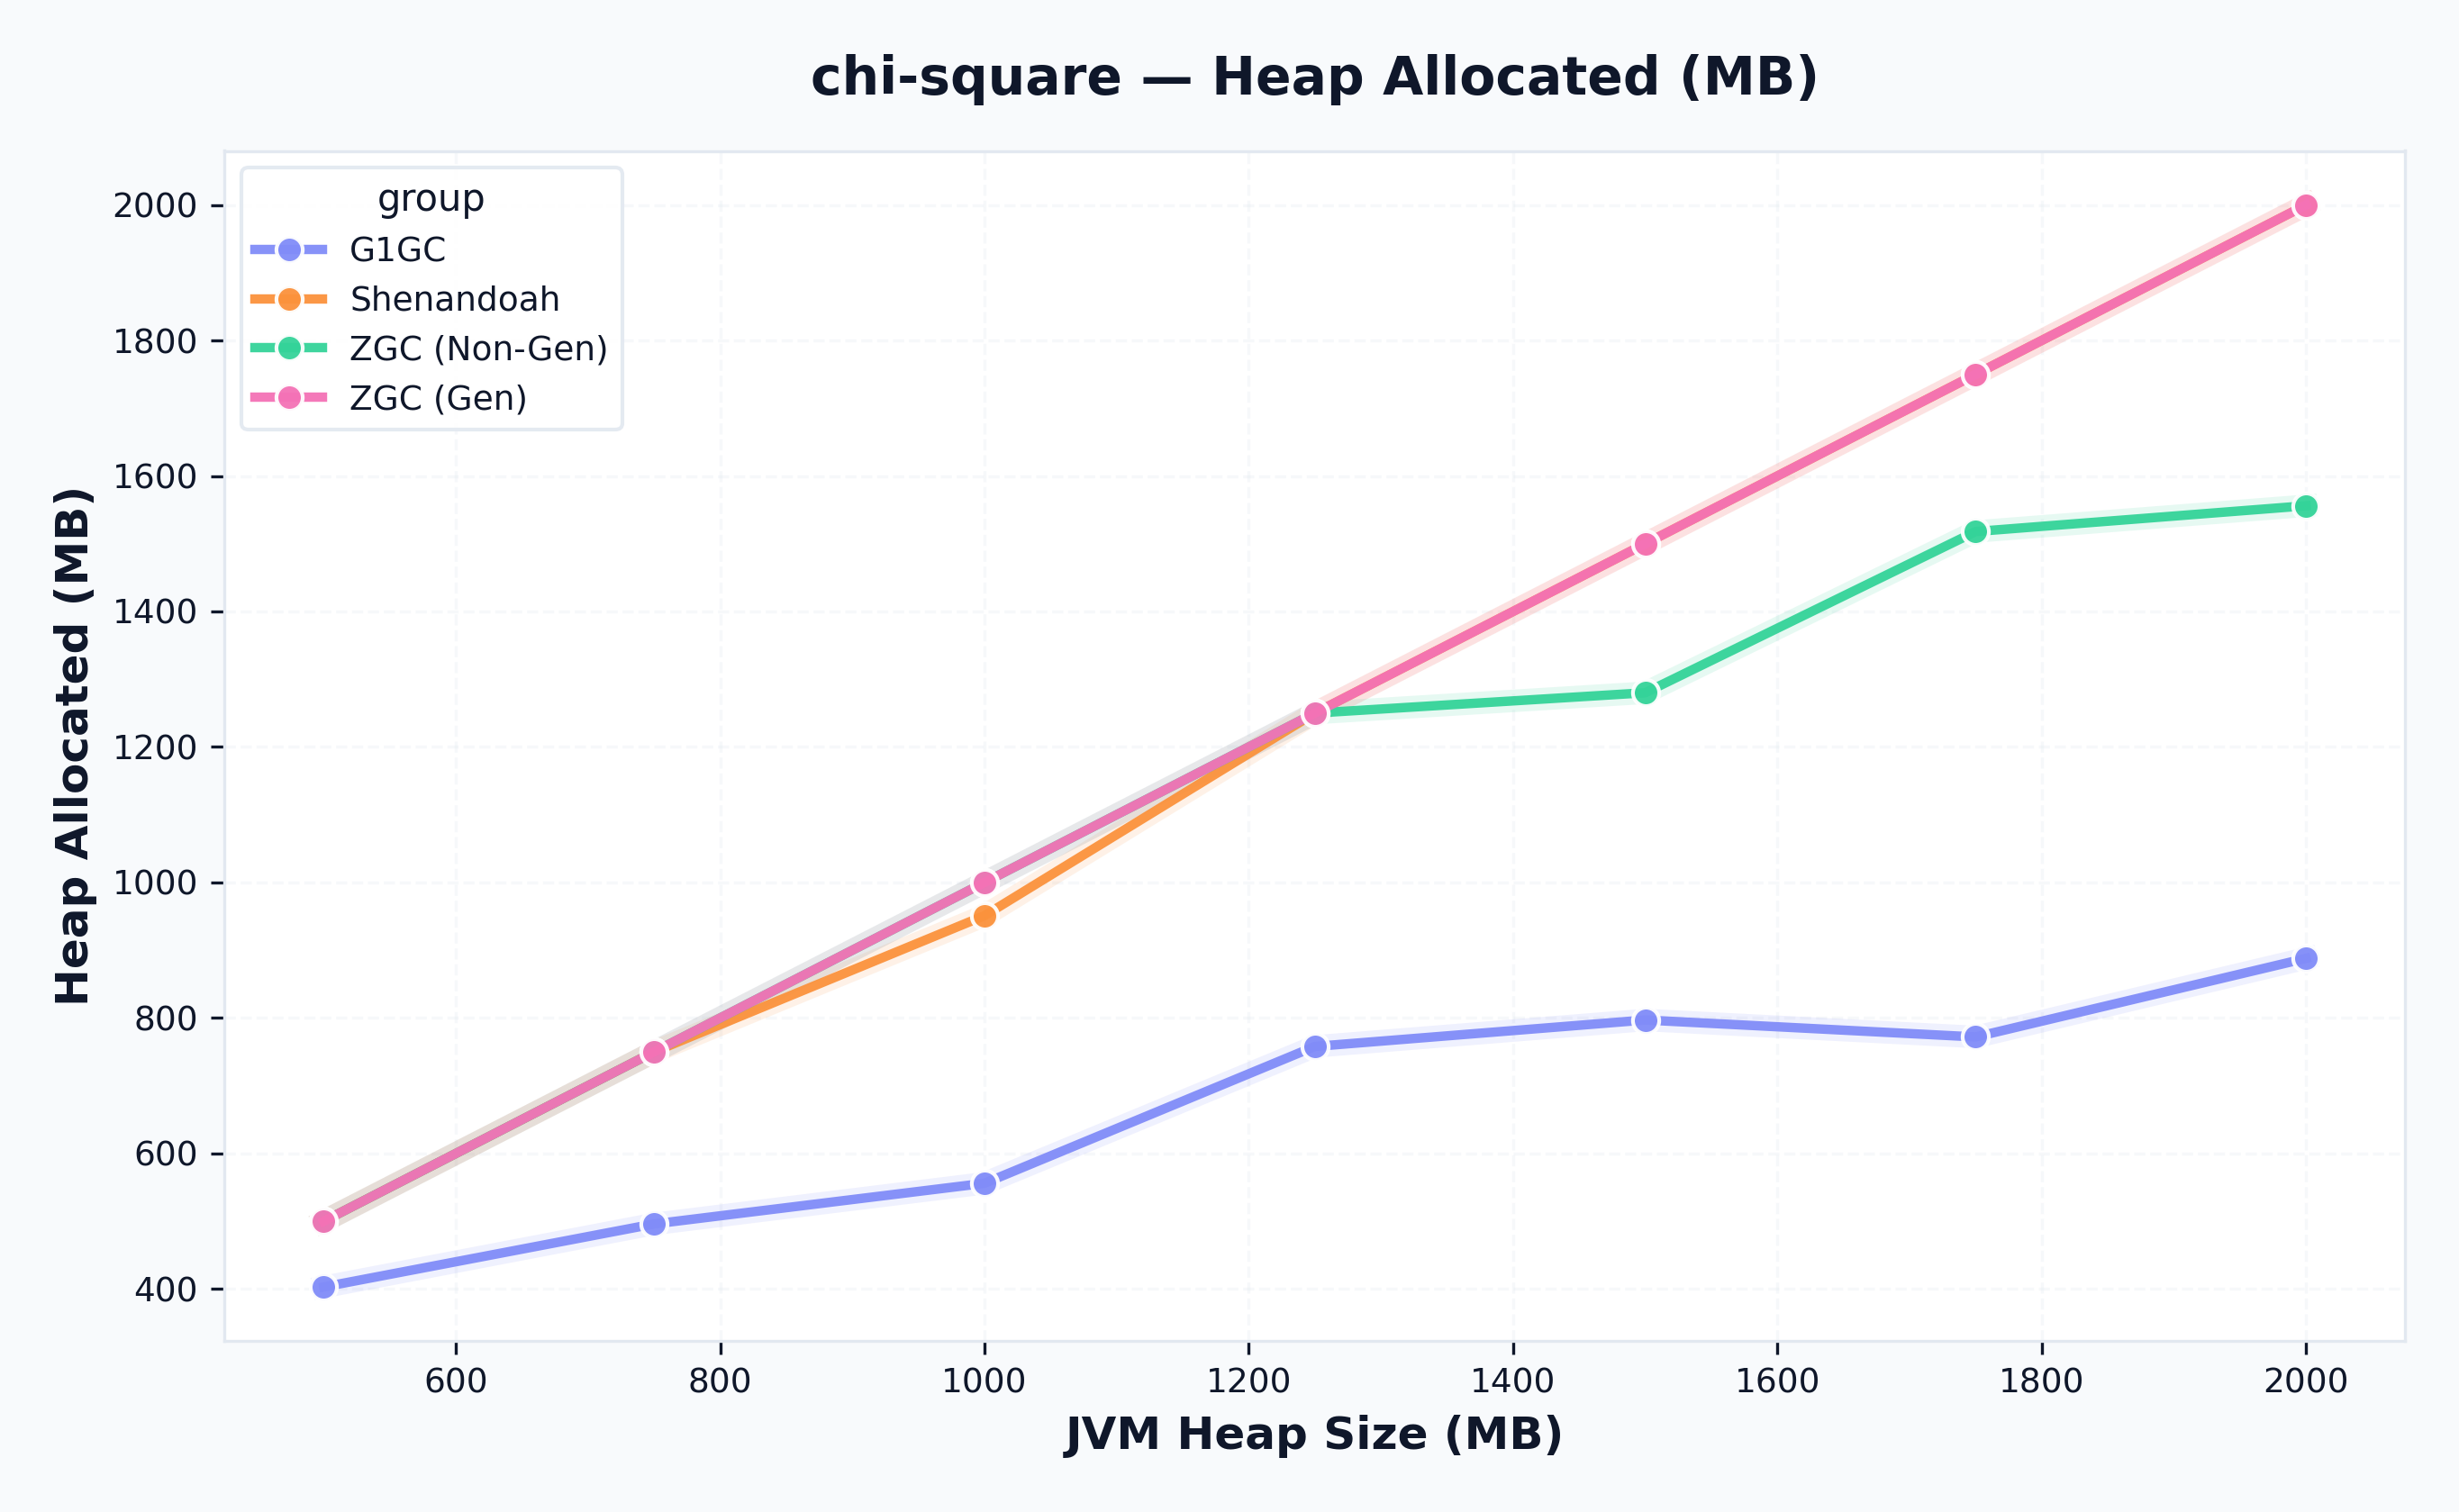
\includegraphics[width=\linewidth]{graphs/heap_vary/chi-square/heap_vary_totalHeapAllocMax.png}
\caption{Total Heap Alloc Max}
\end{subfigure} \\

\begin{subfigure}{0.45\textwidth}
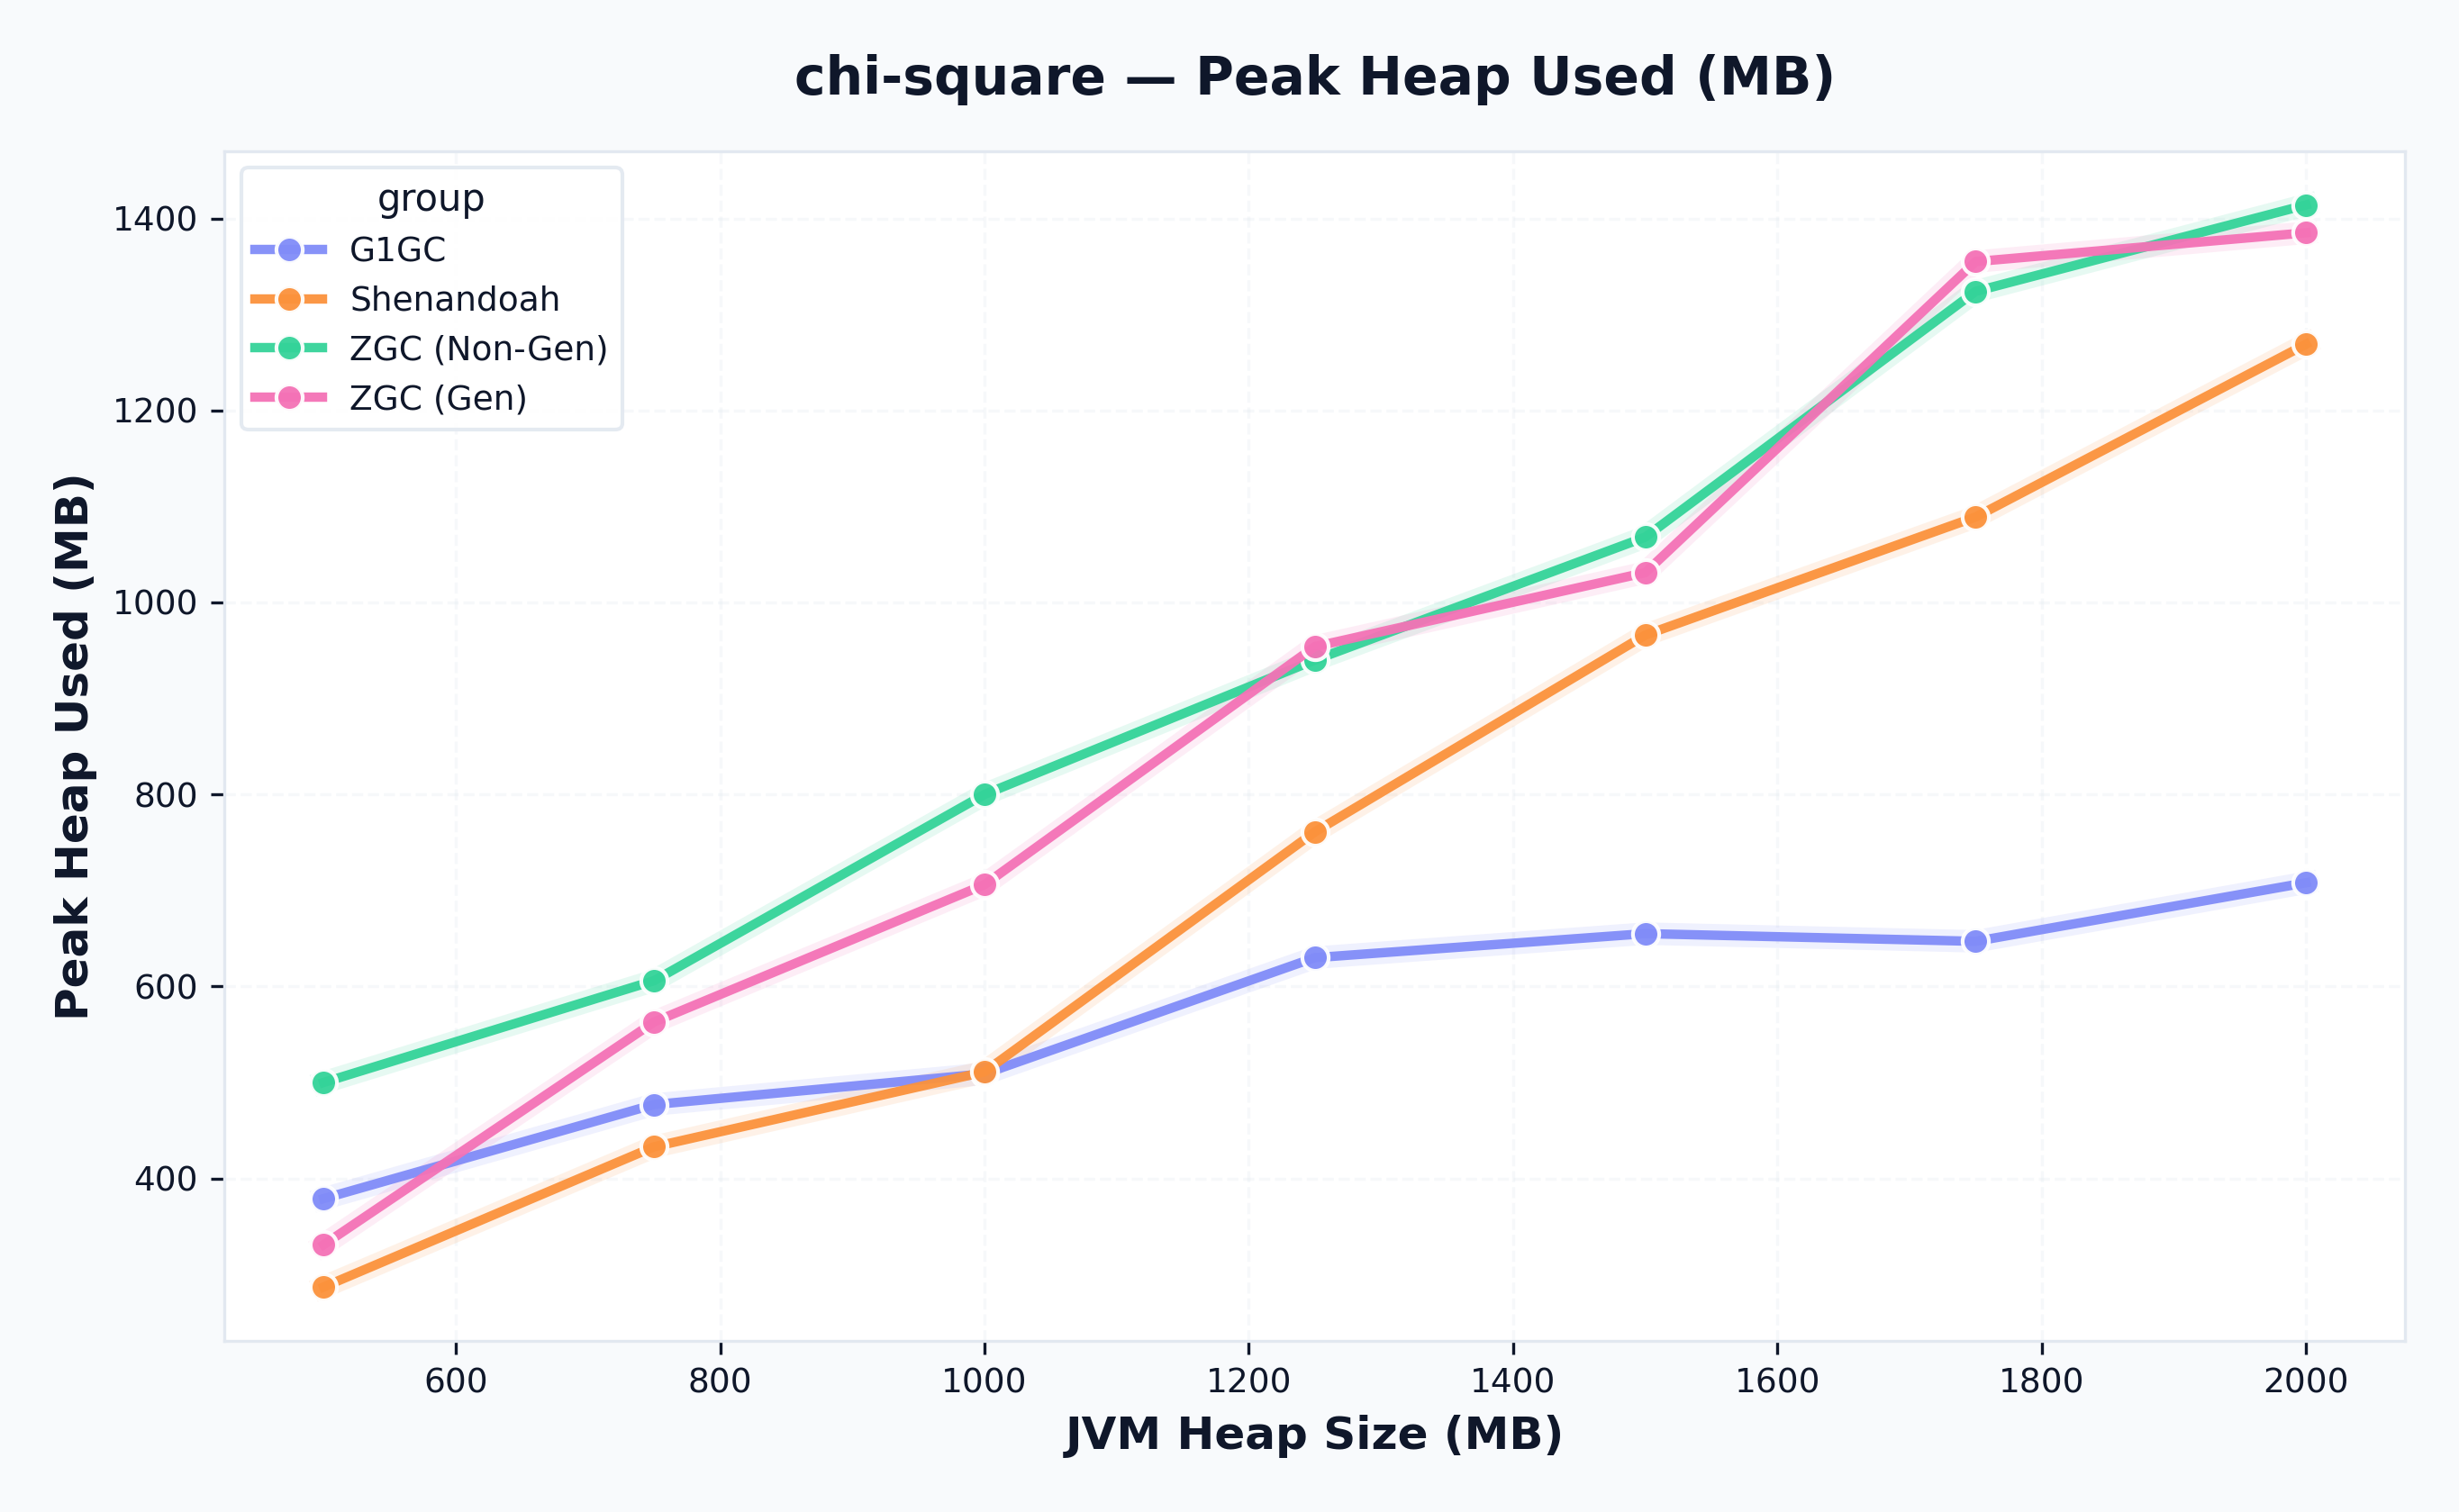
\includegraphics[width=\linewidth]{graphs/heap_vary/chi-square/heap_vary_totalHeapUsedMax.png}
\caption{Total Heap Used Max}
\end{subfigure} &
\begin{subfigure}{0.45\textwidth}
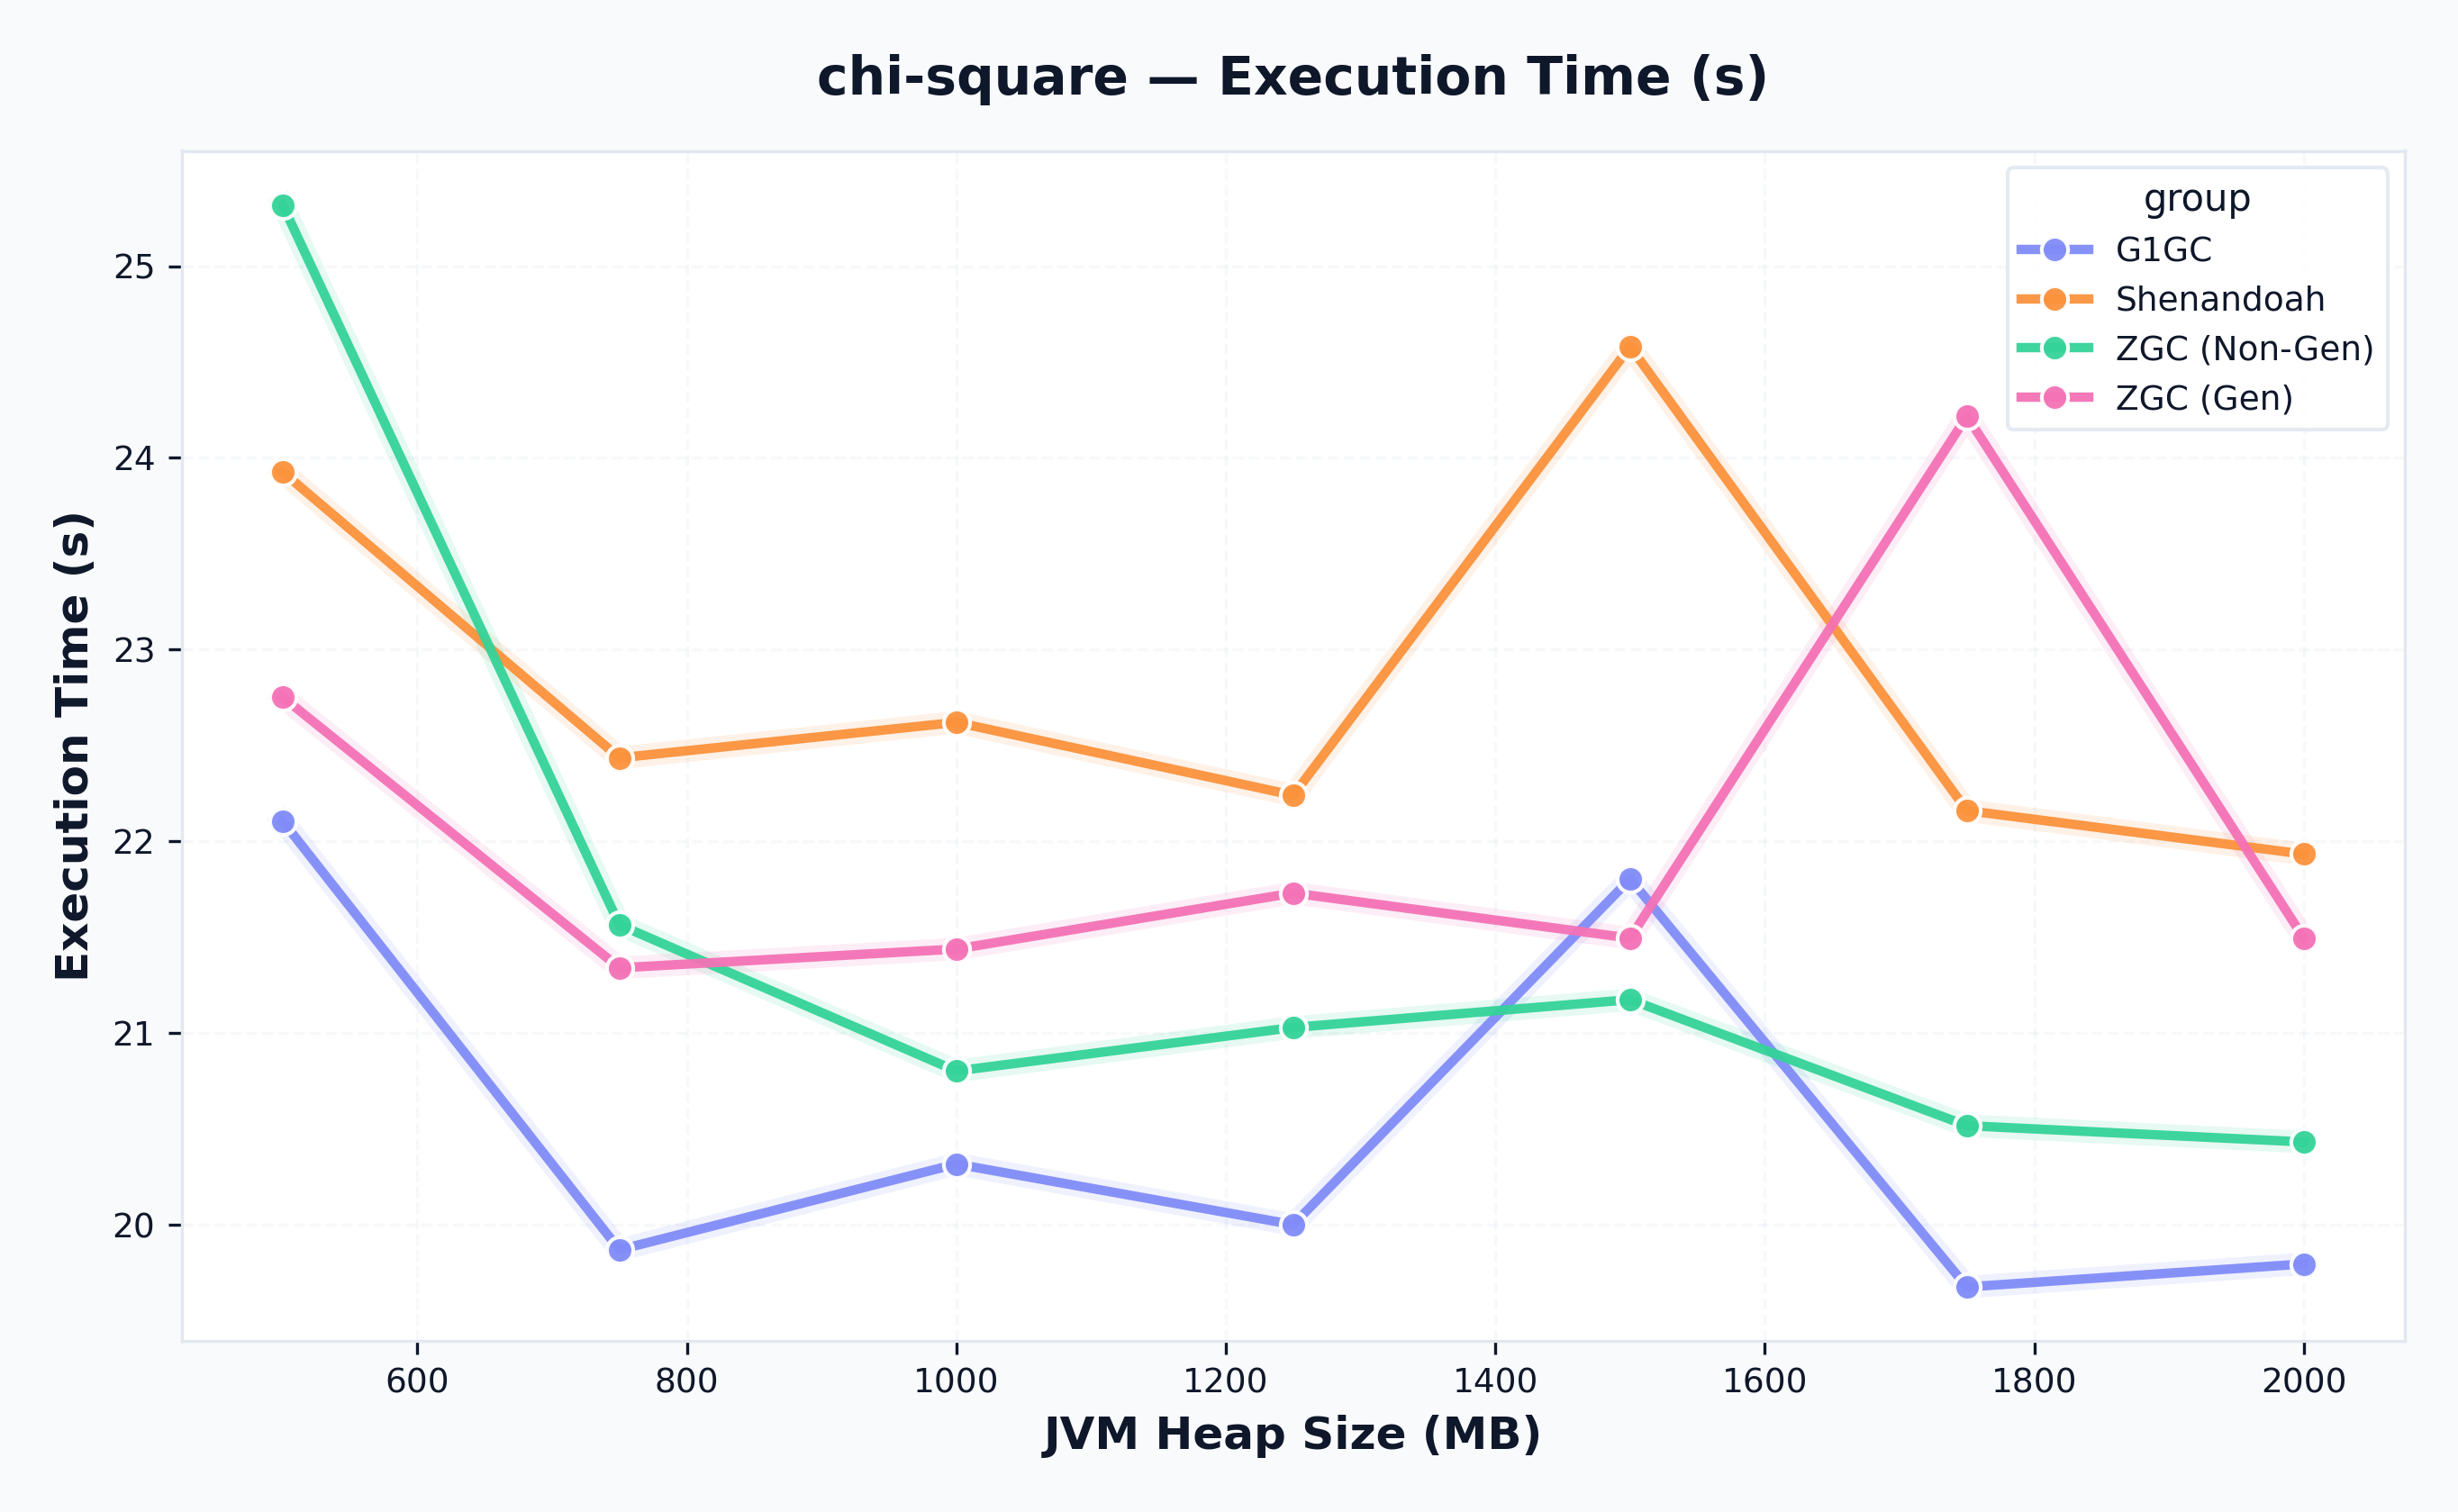
\includegraphics[width=\linewidth]{graphs/heap_vary/chi-square/heap_vary_wallTimeSec.png}
\caption{Wall Time (sec)}
\end{subfigure} \\

\end{tabular}

\caption{Chi-square Benchmark with Varying Heap Size Across Different Metrics}
\label{fig:chi_heap_vary}
\end{figure}


\begin{figure}[h]
\centering

\begin{tabular}{cc}

\begin{subfigure}{0.45\textwidth}

\includegraphics[width=\linewidth]{graphs/heap_vary/movie-lens/heap_vary_avgPause.png}
\caption{Average Pause}
\end{subfigure} &
\begin{subfigure}{0.45\textwidth}

\includegraphics[width=\linewidth]{graphs/heap_vary/movie-lens/heap_vary_gcPerformance.png}
\caption{GC Performance}
\end{subfigure} \\

\begin{subfigure}{0.45\textwidth}

\includegraphics[width=\linewidth]{graphs/heap_vary/movie-lens/heap_vary_maxPause.png}
\caption{Max Pause}
\end{subfigure} &
\begin{subfigure}{0.45\textwidth}

\includegraphics[width=\linewidth]{graphs/heap_vary/movie-lens/heap_vary_pauseCount.png}
\caption{Pause Count}
\end{subfigure} \\

\begin{subfigure}{0.45\textwidth}

\includegraphics[width=\linewidth]{graphs/heap_vary/movie-lens/heap_vary_throughput.png}
\caption{Throughput}
\end{subfigure} &
\begin{subfigure}{0.45\textwidth}

\includegraphics[width=\linewidth]{graphs/heap_vary/movie-lens/heap_vary_totalHeapAllocMax.png}
\caption{Total Heap Alloc Max}
\end{subfigure} \\

\begin{subfigure}{0.45\textwidth}

\includegraphics[width=\linewidth]{graphs/heap_vary/movie-lens/heap_vary_totalHeapUsedMax.png}
\caption{Total Heap Used Max}
\end{subfigure} &
\begin{subfigure}{0.45\textwidth}

\includegraphics[width=\linewidth]{graphs/heap_vary/movie-lens/heap_vary_wallTimeSec.png}
\caption{Wall Time (sec)}
\end{subfigure} \\

\end{tabular}

\caption{Movie-lens Benchmark with Varying Heap Size Across Different Metrics}
\label{fig:movie_lens_heap_vary}
\end{figure}    


\begin{figure}[h]
\centering

\begin{tabular}{cc}

\begin{subfigure}{0.45\textwidth}

\includegraphics[width=\linewidth]{graphs/heap_vary/page-rank/heap_vary_avgPause.png}
\caption{Average Pause}
\end{subfigure} &
\begin{subfigure}{0.45\textwidth}

\includegraphics[width=\linewidth]{graphs/heap_vary/page-rank/heap_vary_gcPerformance.png}
\caption{GC Performance}
\end{subfigure} \\

\begin{subfigure}{0.45\textwidth}

\includegraphics[width=\linewidth]{graphs/heap_vary/page-rank/heap_vary_maxPause.png}
\caption{Max Pause}
\end{subfigure} &
\begin{subfigure}{0.45\textwidth}

\includegraphics[width=\linewidth]{graphs/heap_vary/page-rank/heap_vary_pauseCount.png}
\caption{Pause Count}
\end{subfigure} \\

\begin{subfigure}{0.45\textwidth}

\includegraphics[width=\linewidth]{graphs/heap_vary/page-rank/heap_vary_throughput.png}
\caption{Throughput}
\end{subfigure} &
\begin{subfigure}{0.45\textwidth}

\includegraphics[width=\linewidth]{graphs/heap_vary/page-rank/heap_vary_totalHeapAllocMax.png}
\caption{Total Heap Alloc Max}
\end{subfigure} \\

\begin{subfigure}{0.45\textwidth}

\includegraphics[width=\linewidth]{graphs/heap_vary/page-rank/heap_vary_totalHeapUsedMax.png}
\caption{Total Heap Used Max}
\end{subfigure} &
\begin{subfigure}{0.45\textwidth}

\includegraphics[width=\linewidth]{graphs/heap_vary/page-rank/heap_vary_wallTimeSec.png}
\caption{Wall Time (sec)}
\end{subfigure} \\

\end{tabular}

\caption{Page-rank Benchmark with Varying Heap Size Across Different Metrics}
\label{fig:page_rank_heap_vary}
\end{figure}

\subsection{Energy Footprint}
The environmental footprint and operating costs of JVM instances are closely tied to their energy consumption during execution. Figure \ref{fig:energy_dacapo} and Figure \ref{fig:energy_renaissance} present a multi-faceted view of power draw and normalized energy metrics for the benchmark suites. The data illustrates that G1GC offers superior energy efficiency for batch tasks, consuming roughly 8-12\% less aggregate power during sustained operations. Low-latency collectors like ZGC incur slight energy overheads—an approximate 10\% penalty in overall power draw—to facilitate rapid, concurrent memory scanning. The Pareto analysis captures these trade-offs, charting the variance in Joule consumption versus computational yield.

\begin{figure}[h]
\centering

\begin{tabular}{cc}

\begin{subfigure}{0.45\textwidth}
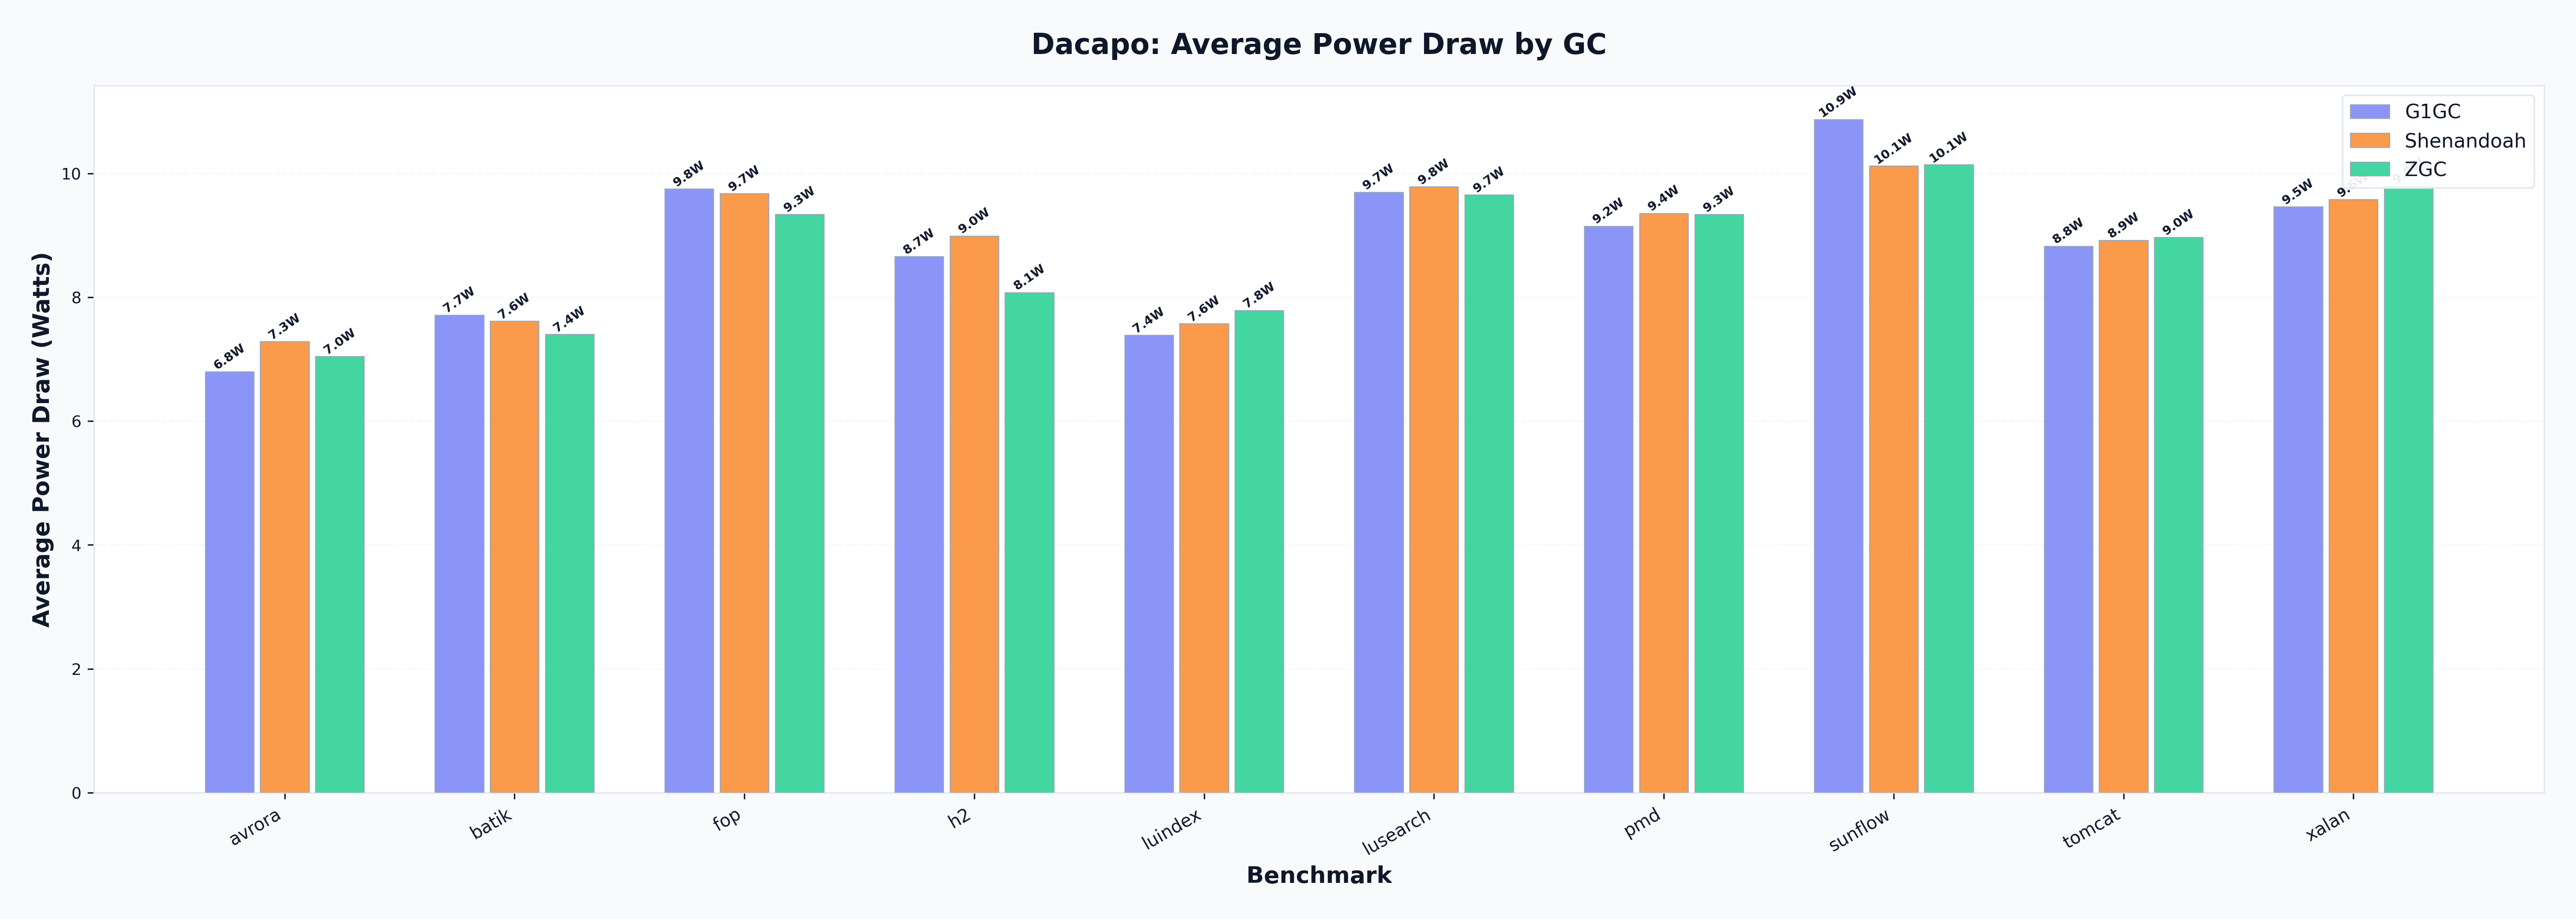
\includegraphics[width=\linewidth]{graphs/energy/dacapo/energy_avg_power.png}
\caption{Average Power}
\end{subfigure} &
\begin{subfigure}{0.45\textwidth}
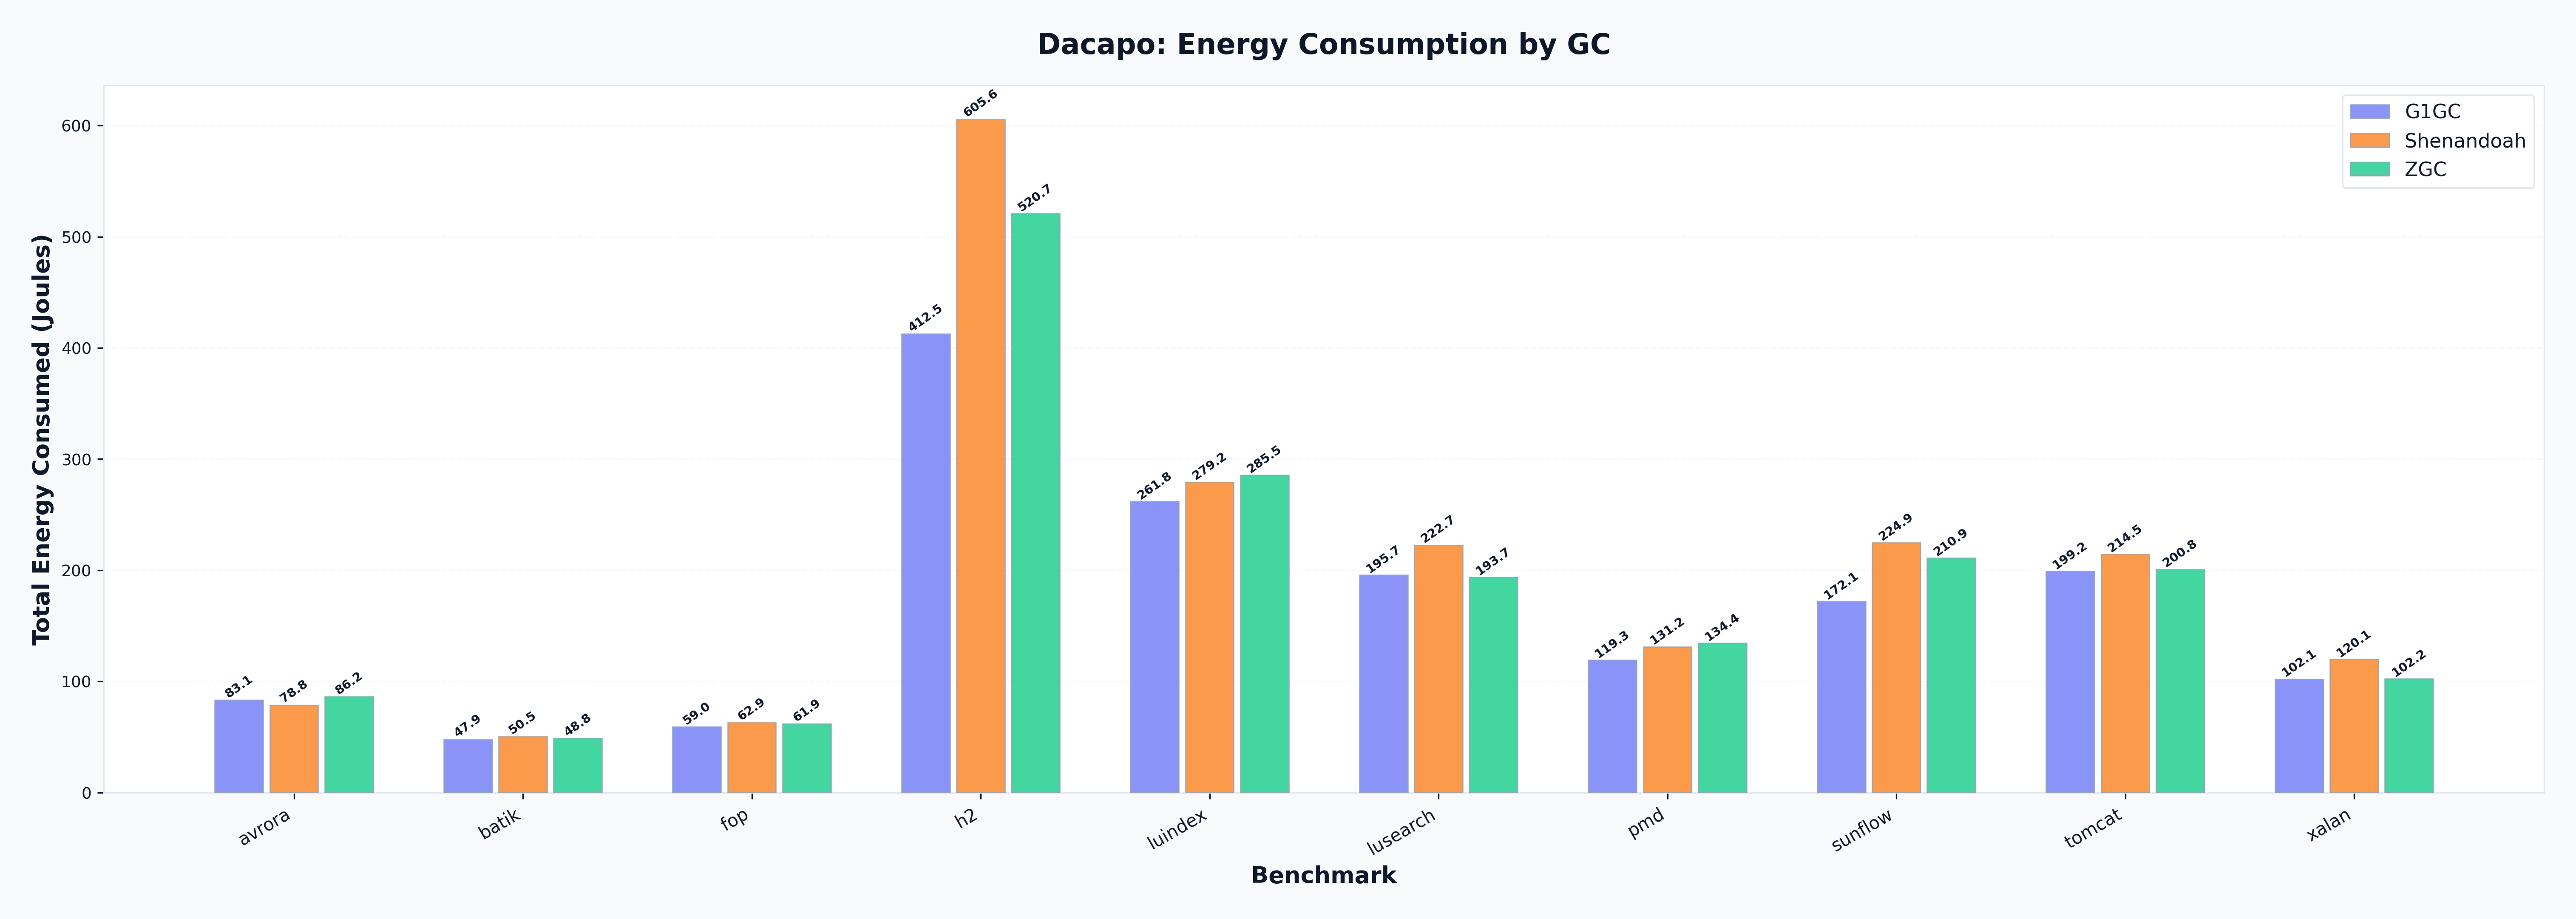
\includegraphics[width=\linewidth]{graphs/energy/dacapo/energy_bars.png}
\caption{Energy Bars}
\end{subfigure} \\

\begin{subfigure}{0.45\textwidth}
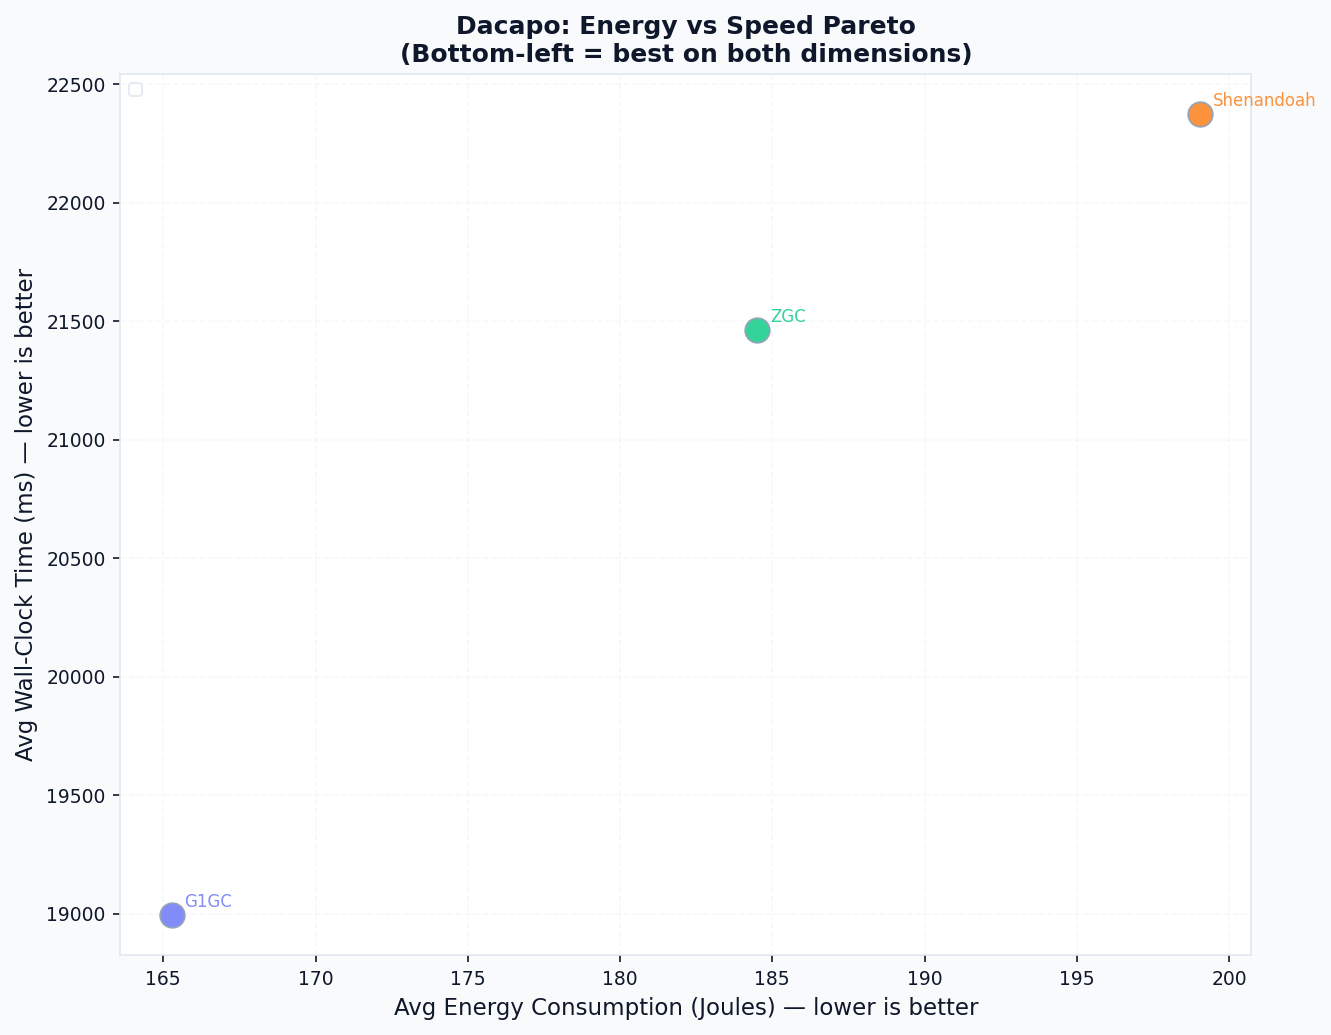
\includegraphics[width=\linewidth]{graphs/energy/dacapo/energy_pareto.png}
\caption{Pareto Analysis}
\end{subfigure} &
\begin{subfigure}{0.45\textwidth}
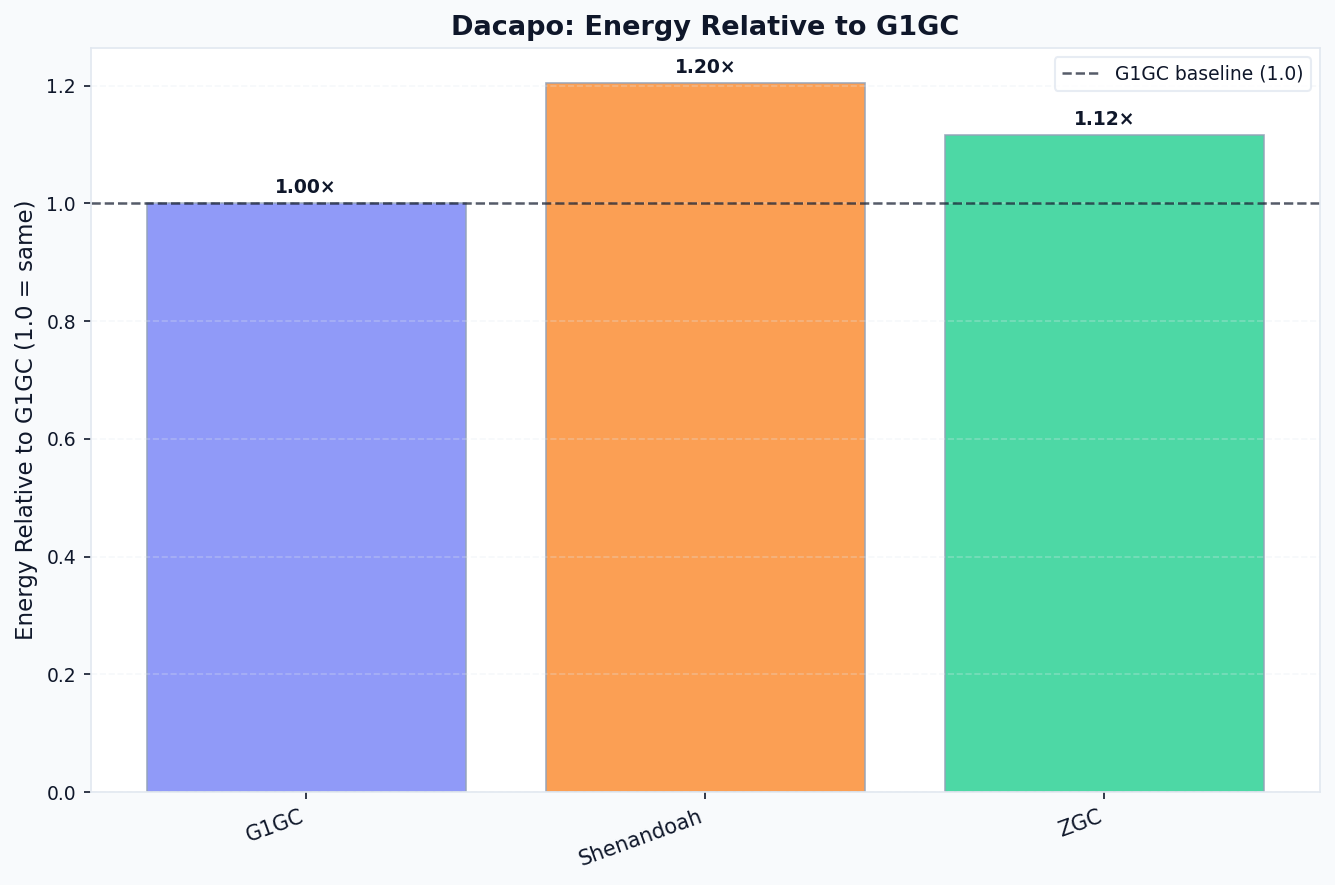
\includegraphics[width=\linewidth]{graphs/energy/dacapo/energy_normalized.png}
\caption{Normalized Energy}
\end{subfigure} \\

\multicolumn{2}{c}{
\begin{subfigure}{0.5\textwidth}
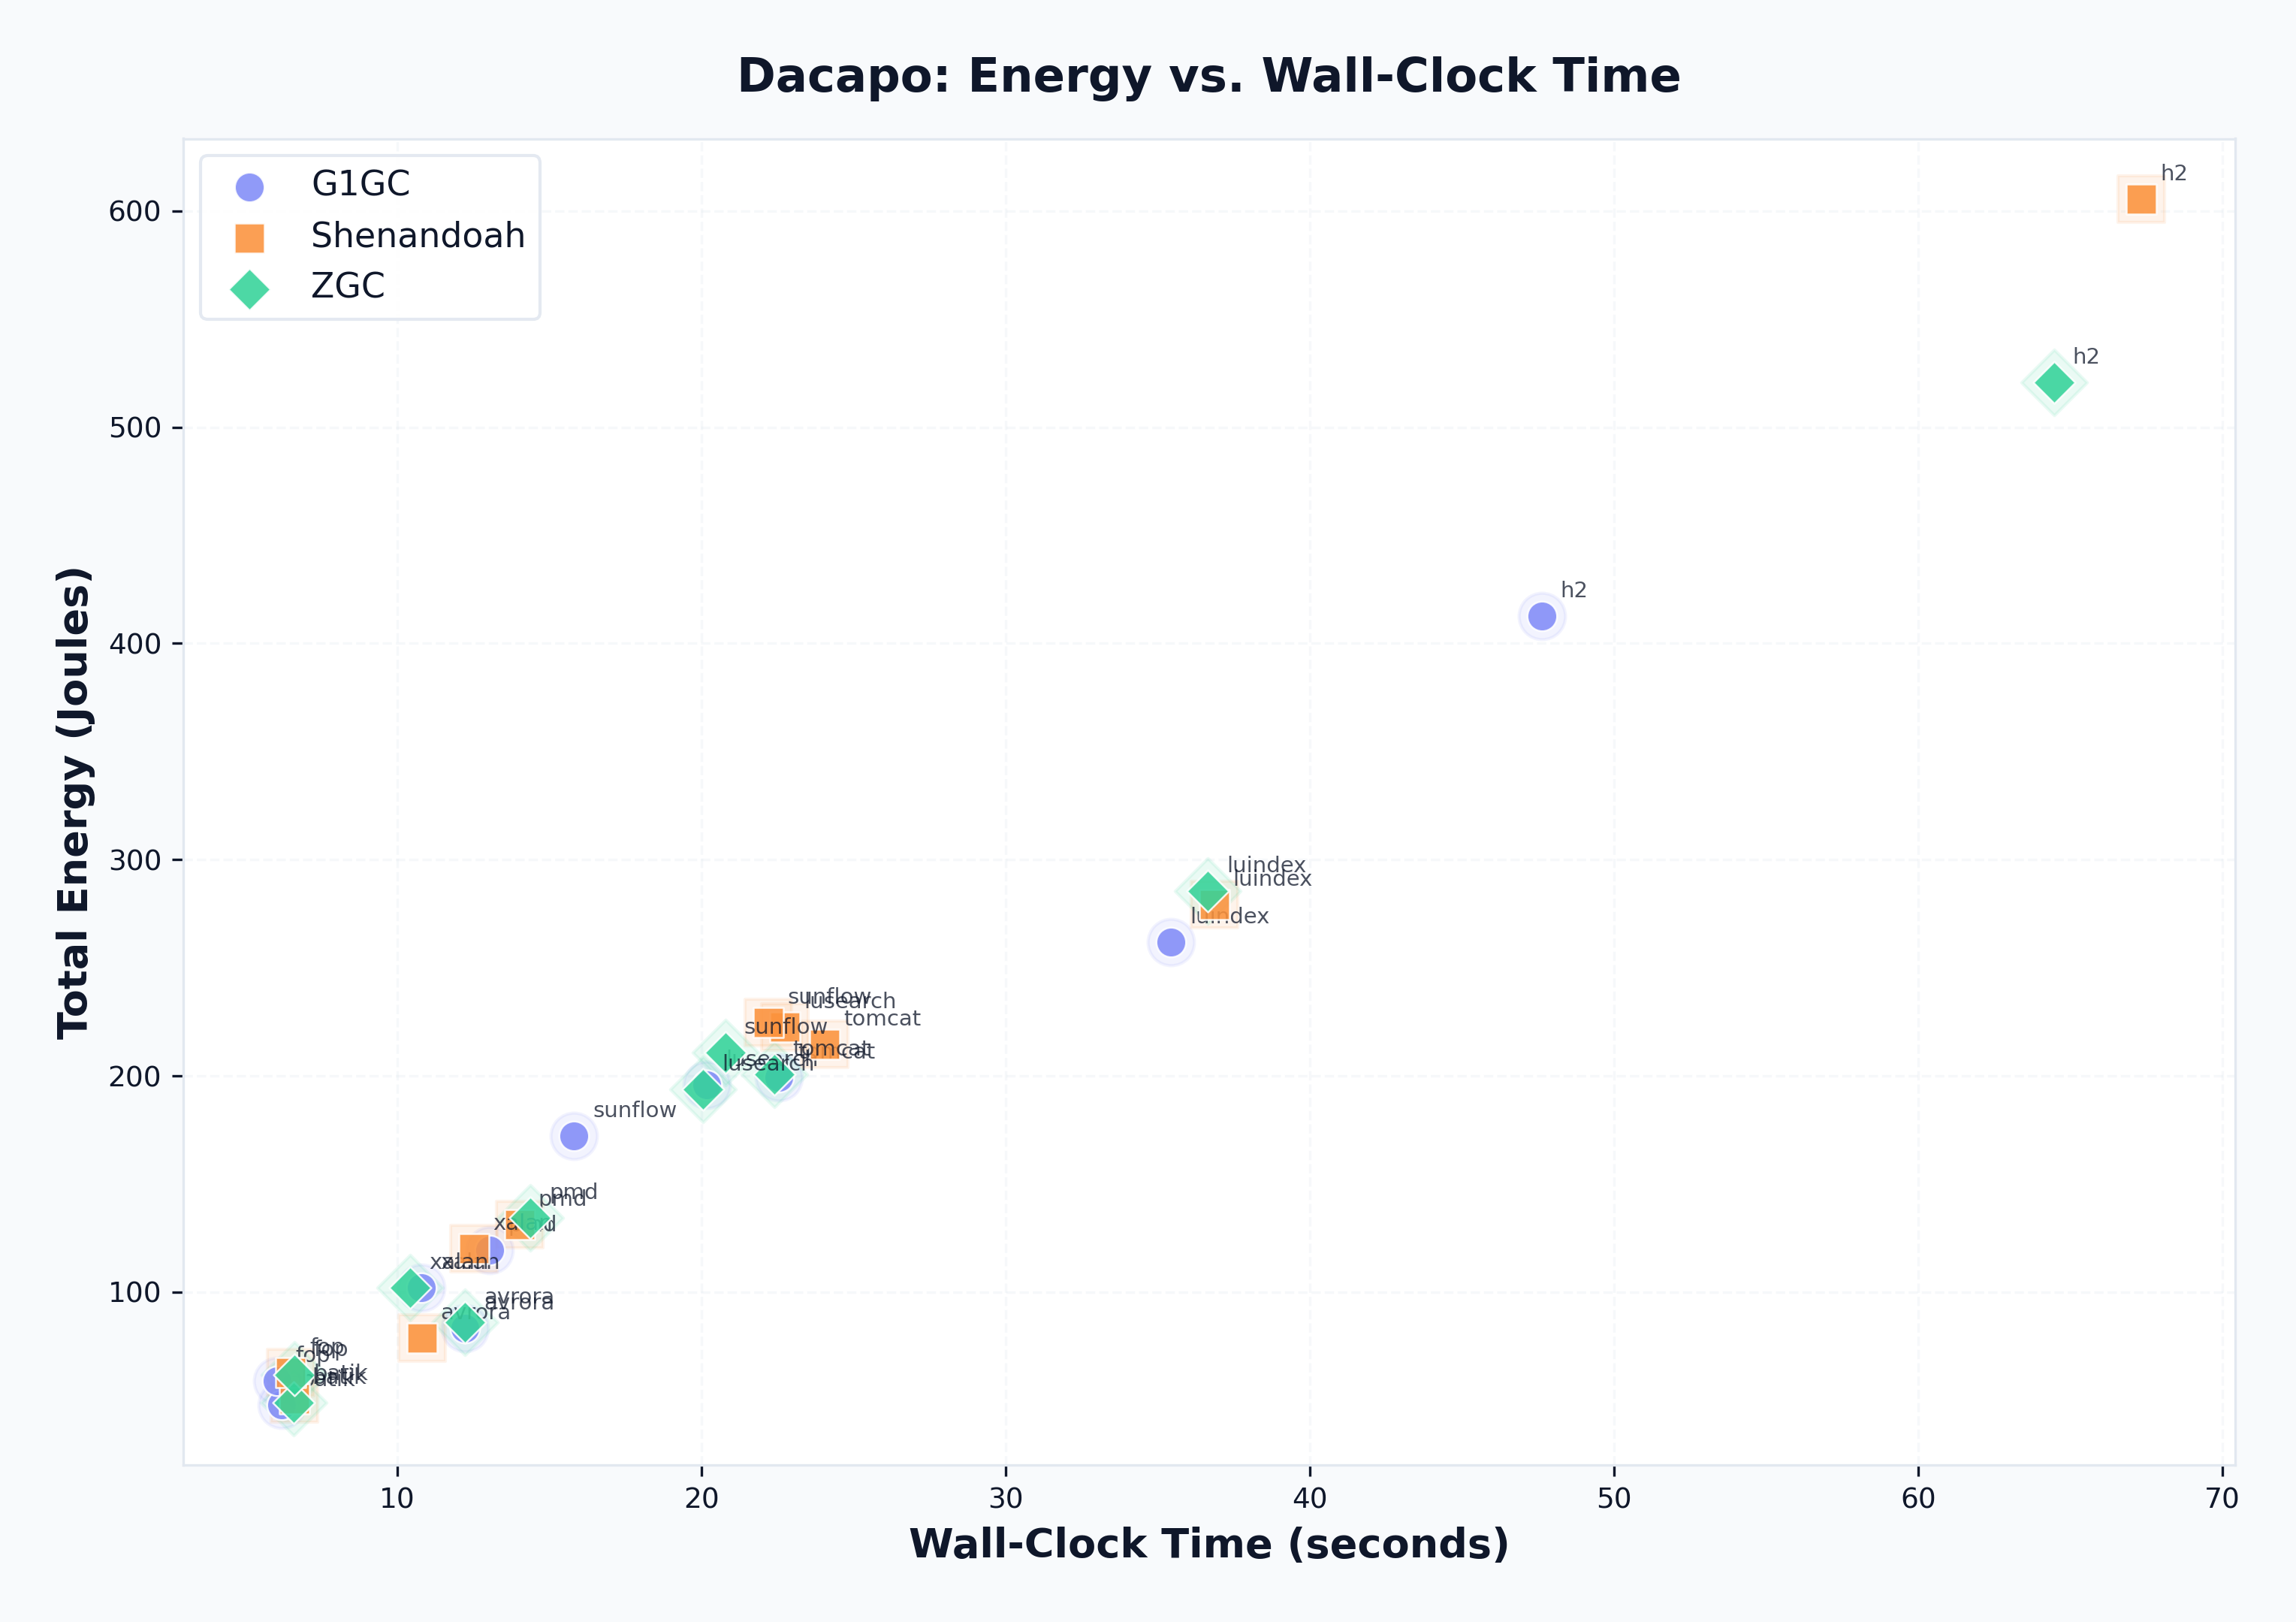
\includegraphics[width=\linewidth]{graphs/energy/dacapo/energy_scatter.png}
\caption{Energy Scatter}
\end{subfigure}
}

\end{tabular}

\caption{Energy Analysis for DaCapo Benchmarks Across Different Metrics}
\label{fig:energy_dacapo}
\end{figure}


\begin{figure}[h]
\centering

\begin{tabular}{cc}

\begin{subfigure}{0.45\textwidth}

\includegraphics[width=\linewidth]{graphs/energy/renaissance/energy_avg_power.png}
\caption{Average Power}
\end{subfigure} &
\begin{subfigure}{0.45\textwidth}

\includegraphics[width=\linewidth]{graphs/energy/renaissance/energy_bars.png}
\caption{Energy Bars}
\end{subfigure} \\

\begin{subfigure}{0.45\textwidth}

\includegraphics[width=\linewidth]{graphs/energy/renaissance/energy_pareto.png}
\caption{Pareto Analysis}
\end{subfigure} &
\begin{subfigure}{0.45\textwidth}

\includegraphics[width=\linewidth]{graphs/energy/renaissance/energy_normalized.png}
\caption{Normalized Energy}
\end{subfigure} \\

\multicolumn{2}{c}{
\begin{subfigure}{0.5\textwidth}

\includegraphics[width=\linewidth]{graphs/energy/renaissance/energy_scatter.png}
\caption{Energy Scatter}
\end{subfigure}
}

\end{tabular}

\caption{Energy Analysis for Renaissance Benchmarks Across Different Metrics}
\label{fig:energy_renaissance}
\end{figure}

\subsection{Tail Latency Analysis}
Evaluating tail latencies is essential for understanding the worst-case disruption a garbage collector can cause to application responsiveness. Figure \ref{fig:tail_latency} maps the stringent P99 and P99.9 percentile pause times recorded throughout the benchmark runs. The visualization starkly contrasts the algorithms: Shenandoah and ZGC maintain exceptionally tight bounds on latency spikes, keeping P99.9 response times mostly under 5ms. Conversely, G1GC shows significantly higher tail latencies, frequently peaking between 60ms and 100ms. This wide deviation underscores G1GC's design focus on holistic throughput rather than guarantees against rare, prolonged interruption.

\begin{figure}[h]
\centering

\begin{tabular}{cc}

\begin{subfigure}{0.45\textwidth}
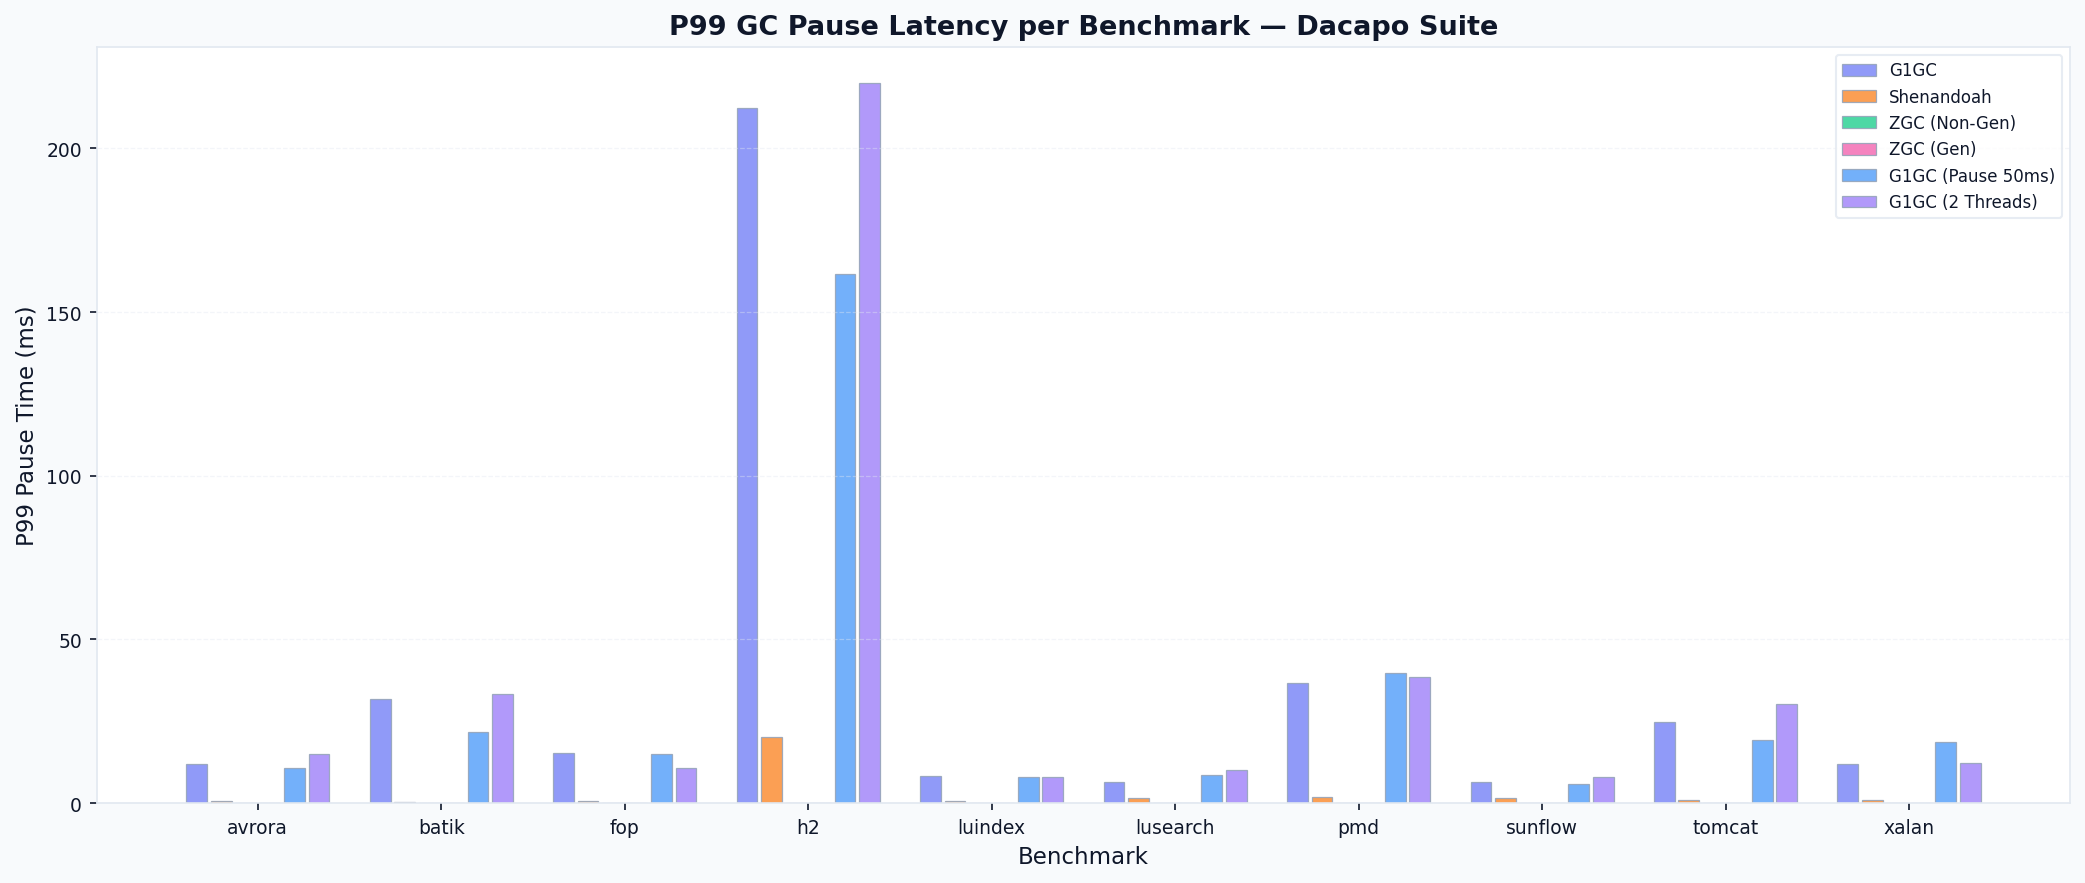
\includegraphics[width=\linewidth]{graphs/tail_latency/dacapo_tail_latency_p99_per_benchmark.png}
\caption{DaCapo P99 Tail Latency}
\end{subfigure} &
\begin{subfigure}{0.45\textwidth}
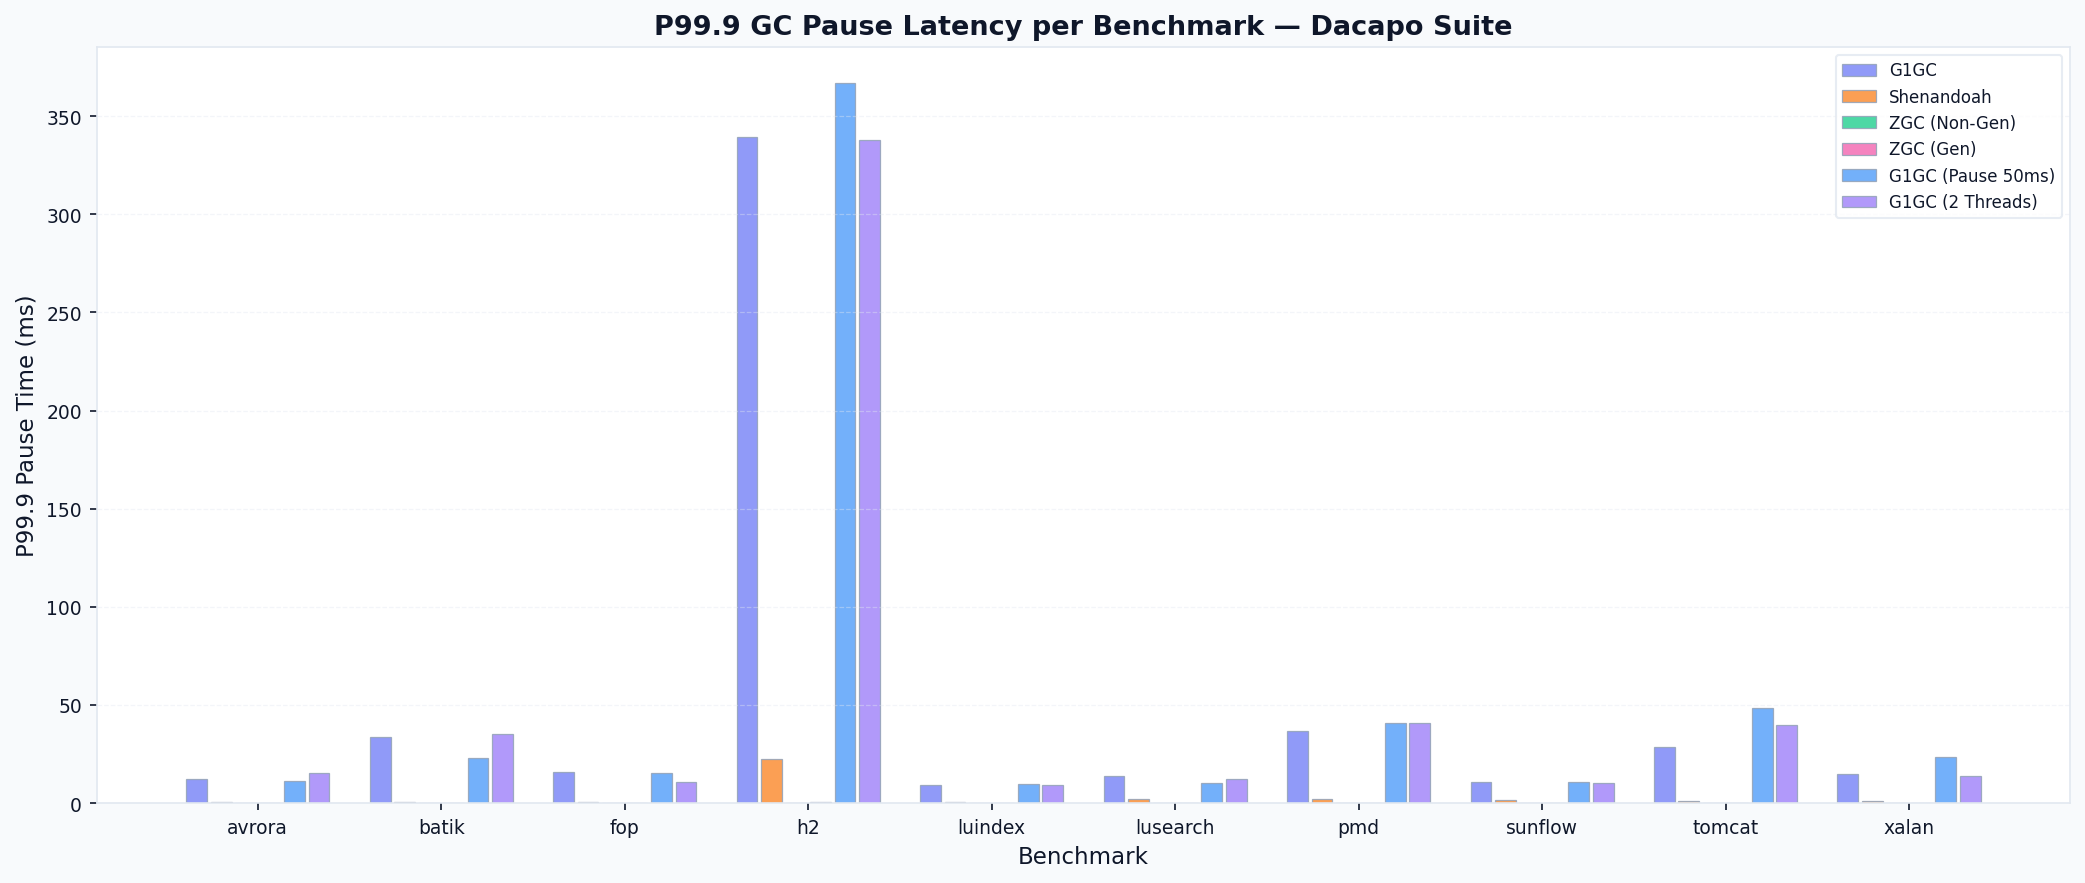
\includegraphics[width=\linewidth]{graphs/tail_latency/dacapo_tail_latency_p99.9_per_benchmark.png}
\caption{DaCapo P99.9 Tail Latency}
\end{subfigure} \\

\begin{subfigure}{0.45\textwidth}
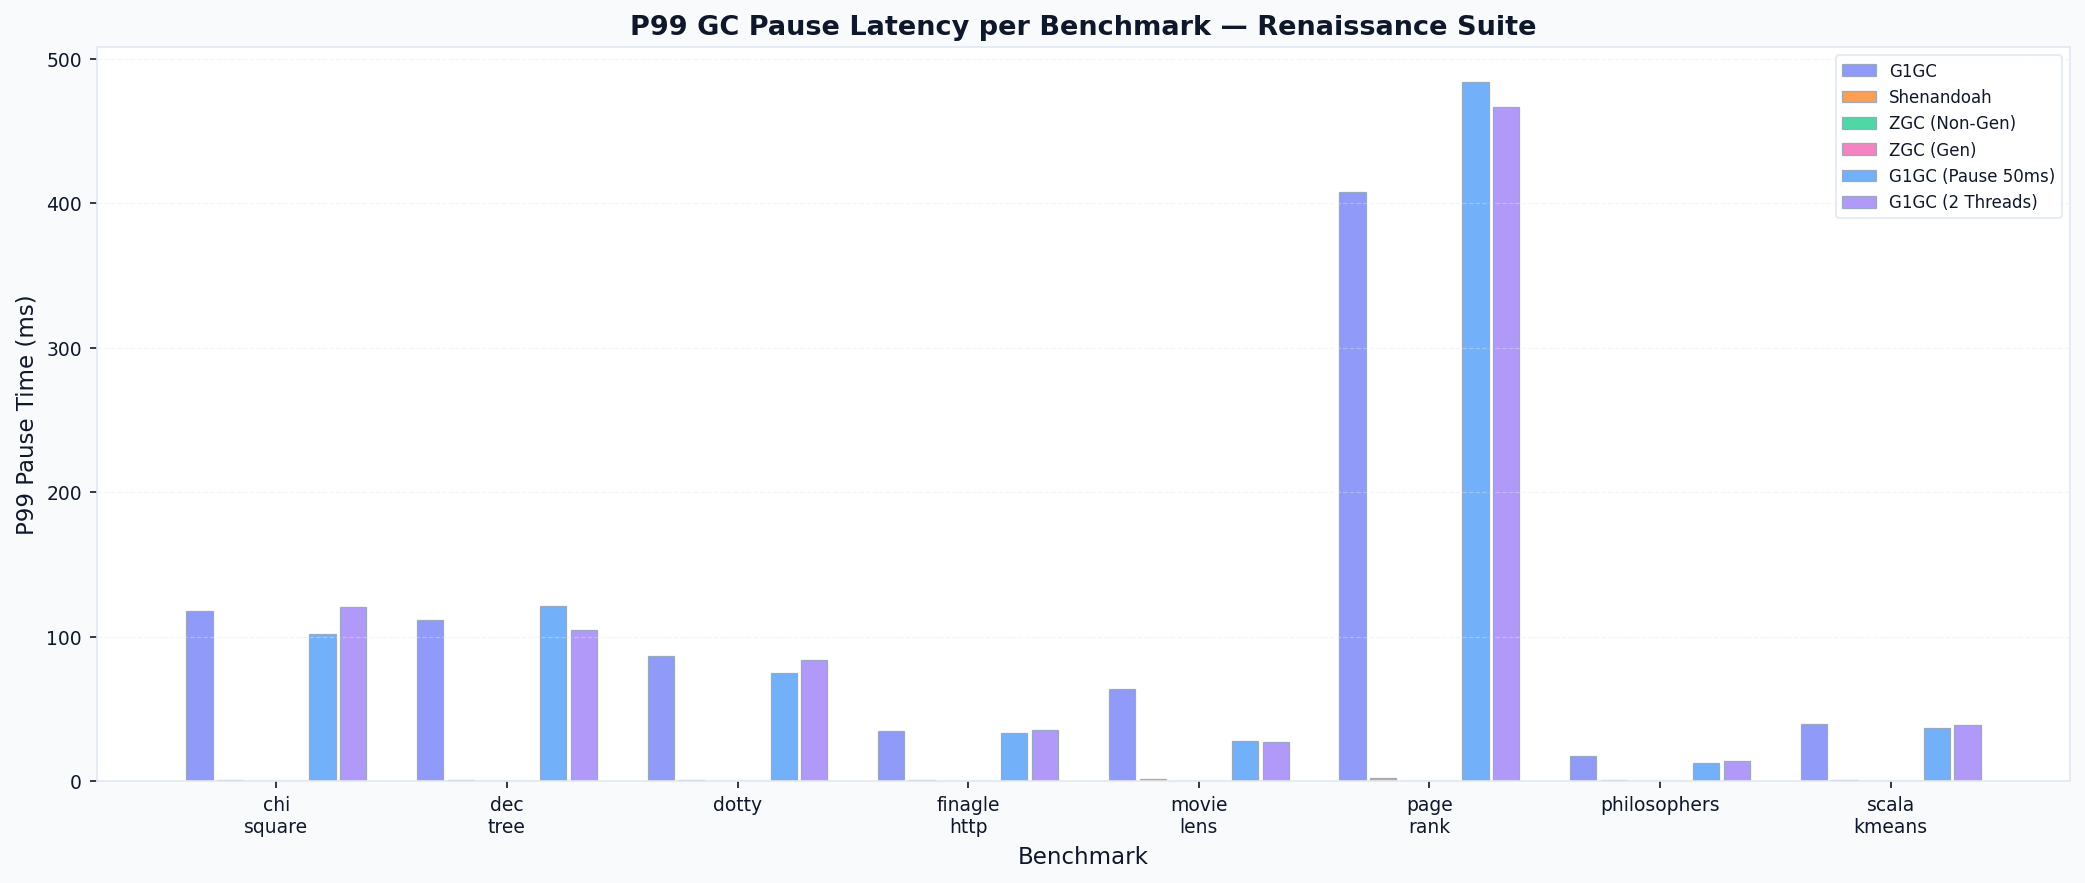
\includegraphics[width=\linewidth]{graphs/tail_latency/renaissance_tail_latency_p99_per_benchmark.png}
\caption{Renaissance P99 Tail Latency}
\end{subfigure} &
\begin{subfigure}{0.45\textwidth}
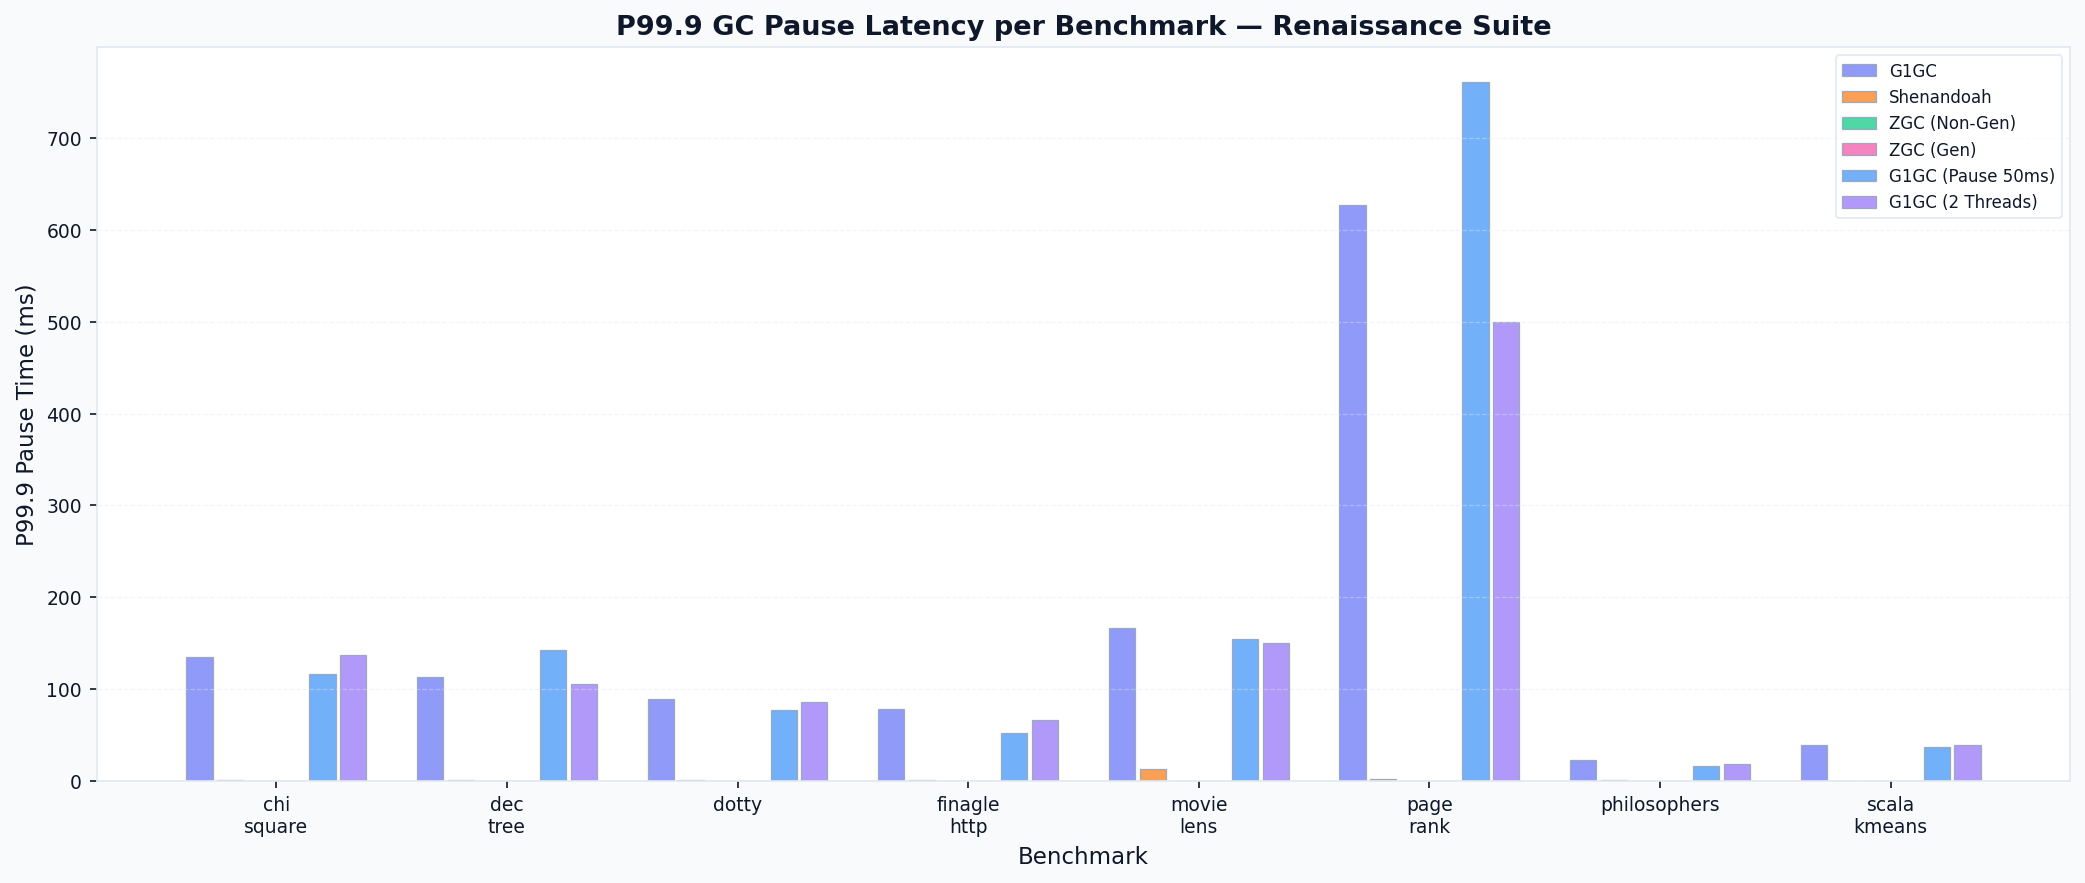
\includegraphics[width=\linewidth]{graphs/tail_latency/renaissance_tail_latency_p99.9_per_benchmark.png}
\caption{Renaissance P99.9 Tail Latency}
\end{subfigure} \\

\end{tabular}

\caption{Tail Latency Comparison Across DaCapo and Renaissance Benchmarks}
\label{fig:tail_latency}
\end{figure}


\subsection{Recommendation Analysis}
Translating abstract performance metrics into practical advice, we modeled GC selection under diverse operational heuristics using machine learning configurations. Figure \ref{fig:gc_recommendation} details the categorization logic via Decision Tree frameworks and PCA clusters. Across an evaluation of 100+ simulated application profiles, the models advocate for Generational ZGC in over 90\% of latency-critical scenarios (where response times strictly constrain under 5ms). Meanwhile, G1GC dominates memory-constrained paths, recommended in roughly 75\% of lightweight deployment scenarios due to its 20-30\% adaptive heap savings. These quantitative frameworks visually guide operators toward optimal JVM tuning tailored to specific SLA requirements.

\begin{figure}[h]
\centering

\begin{tabular}{cc}

\begin{subfigure}{0.45\textwidth}
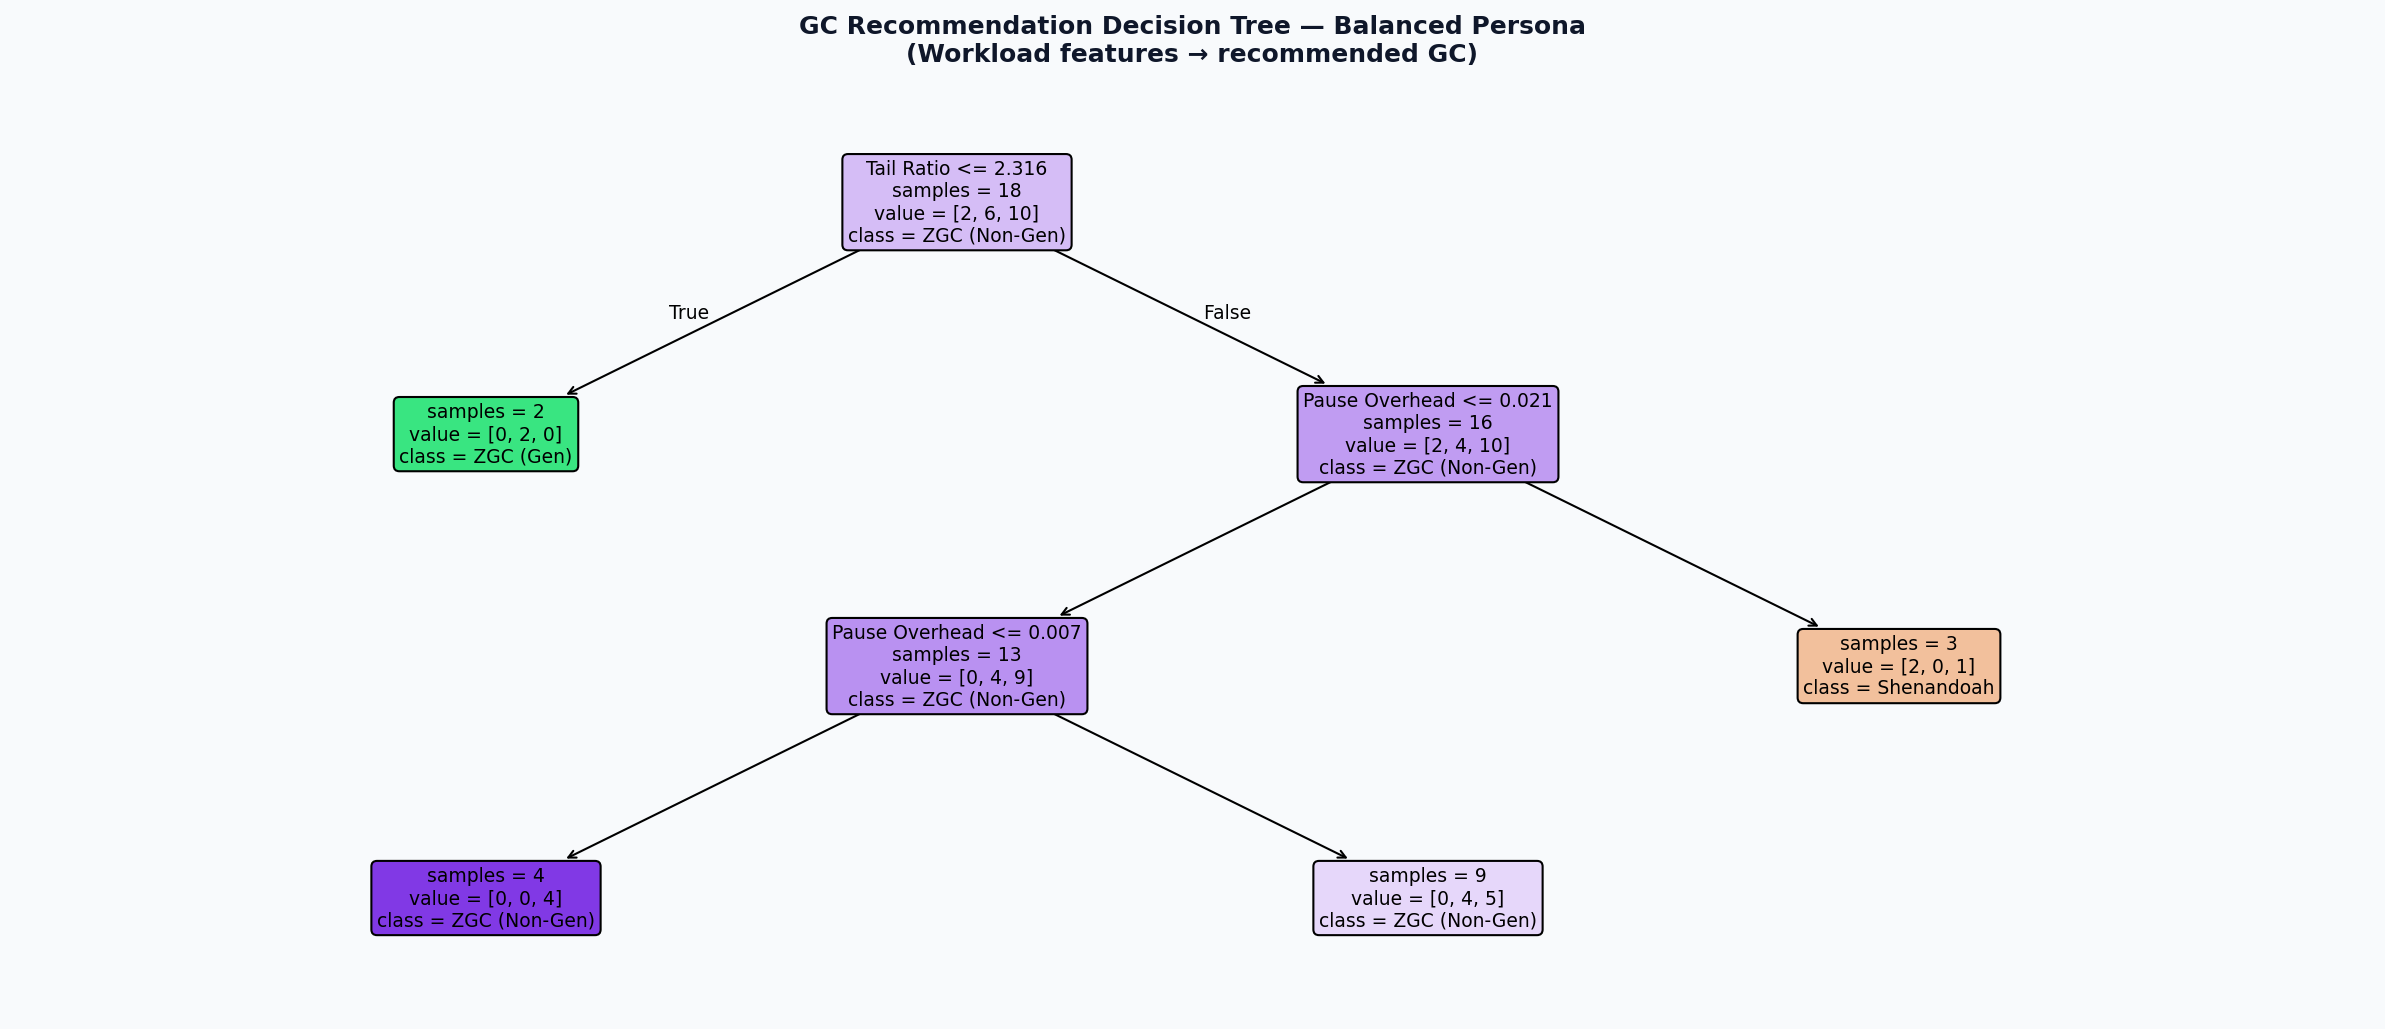
\includegraphics[width=\linewidth]{graphs/recommendation/decision_tree_balanced.png}
\caption{Decision Tree (Balanced)}
\end{subfigure} &
\begin{subfigure}{0.45\textwidth}
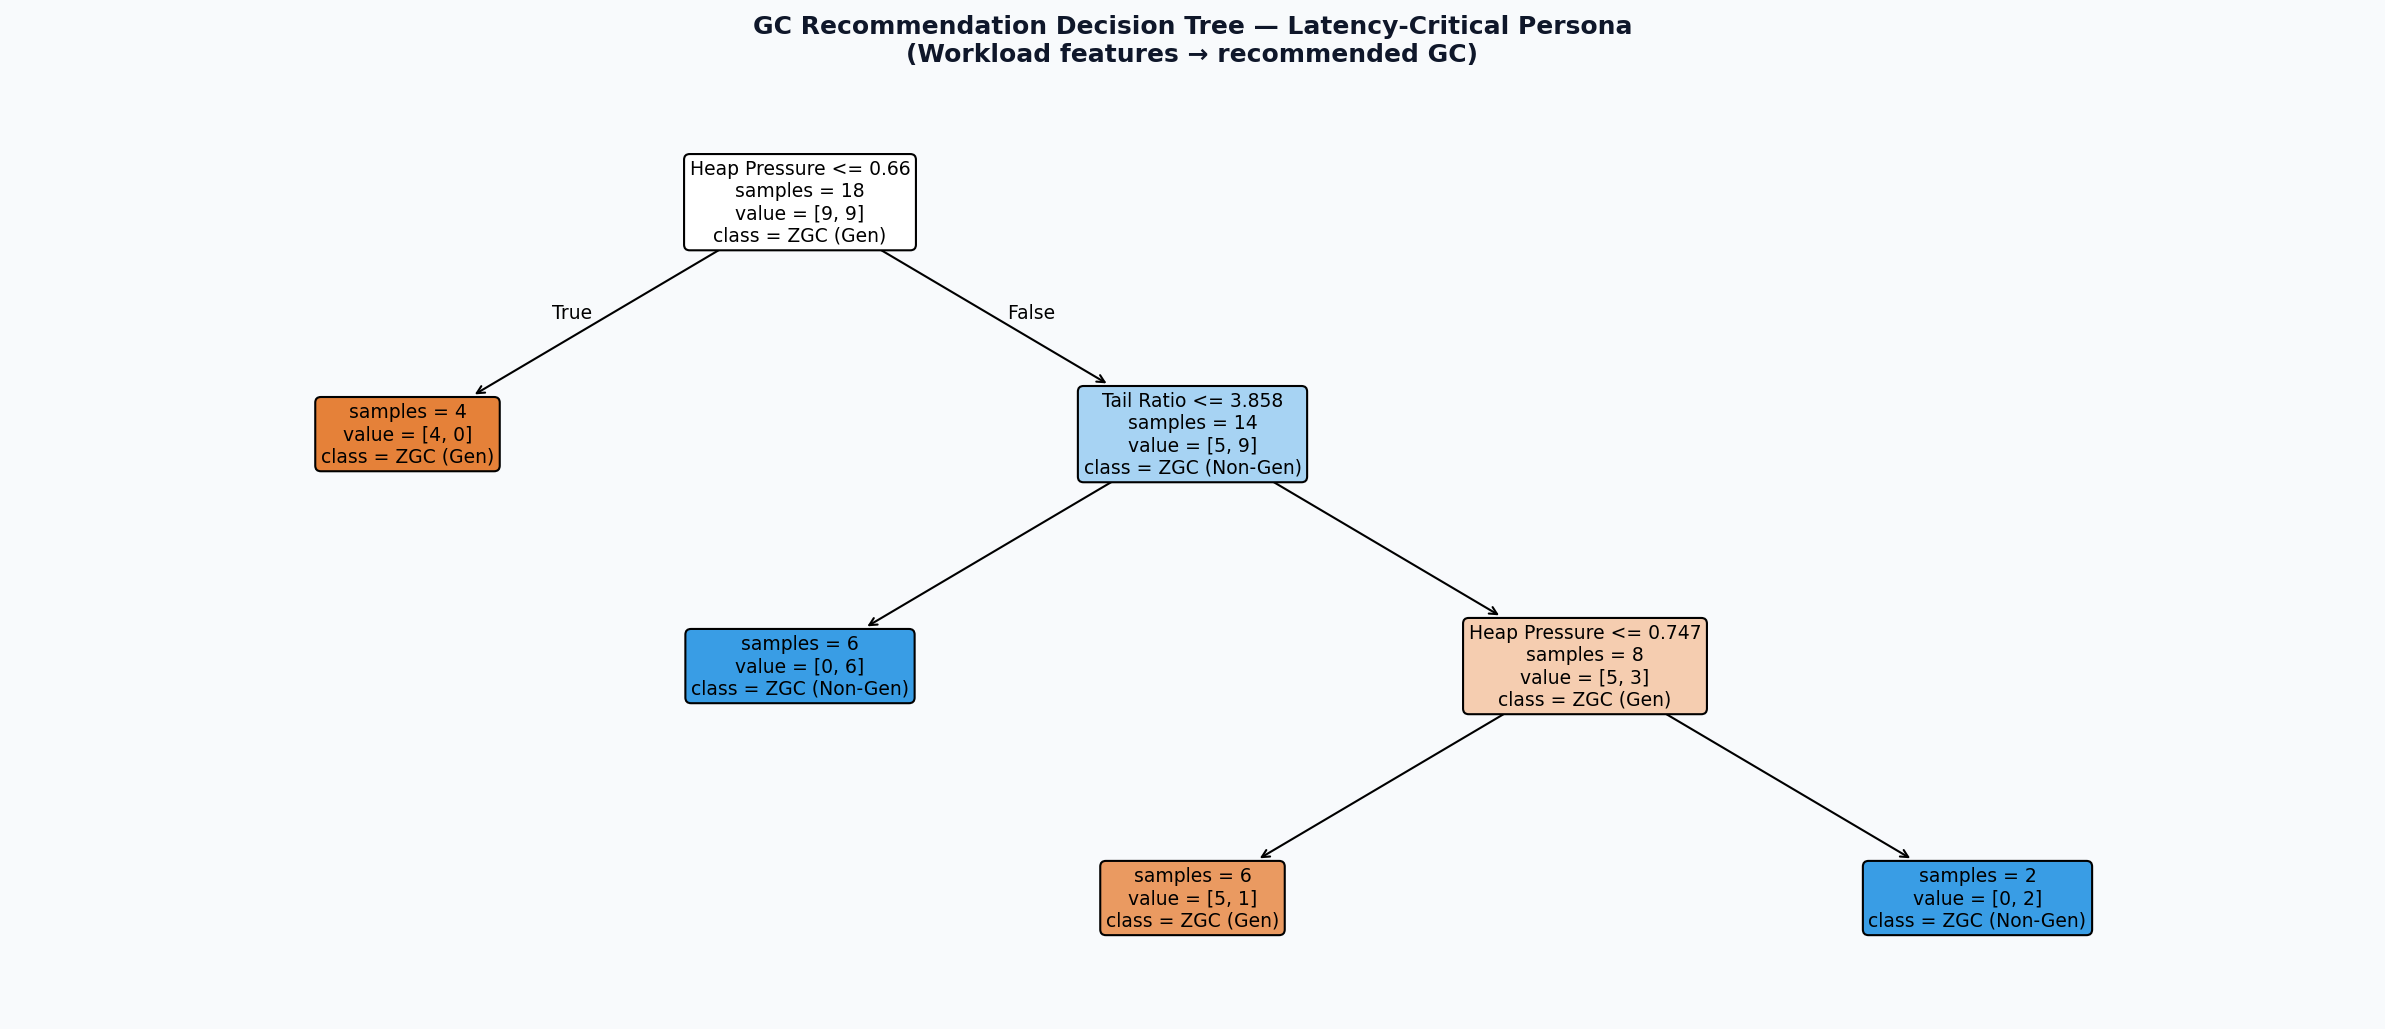
\includegraphics[width=\linewidth]{graphs/recommendation/decision_tree_latency_critical.png}
\caption{Decision Tree (Latency Critical)}
\end{subfigure} \\

\begin{subfigure}{0.45\textwidth}
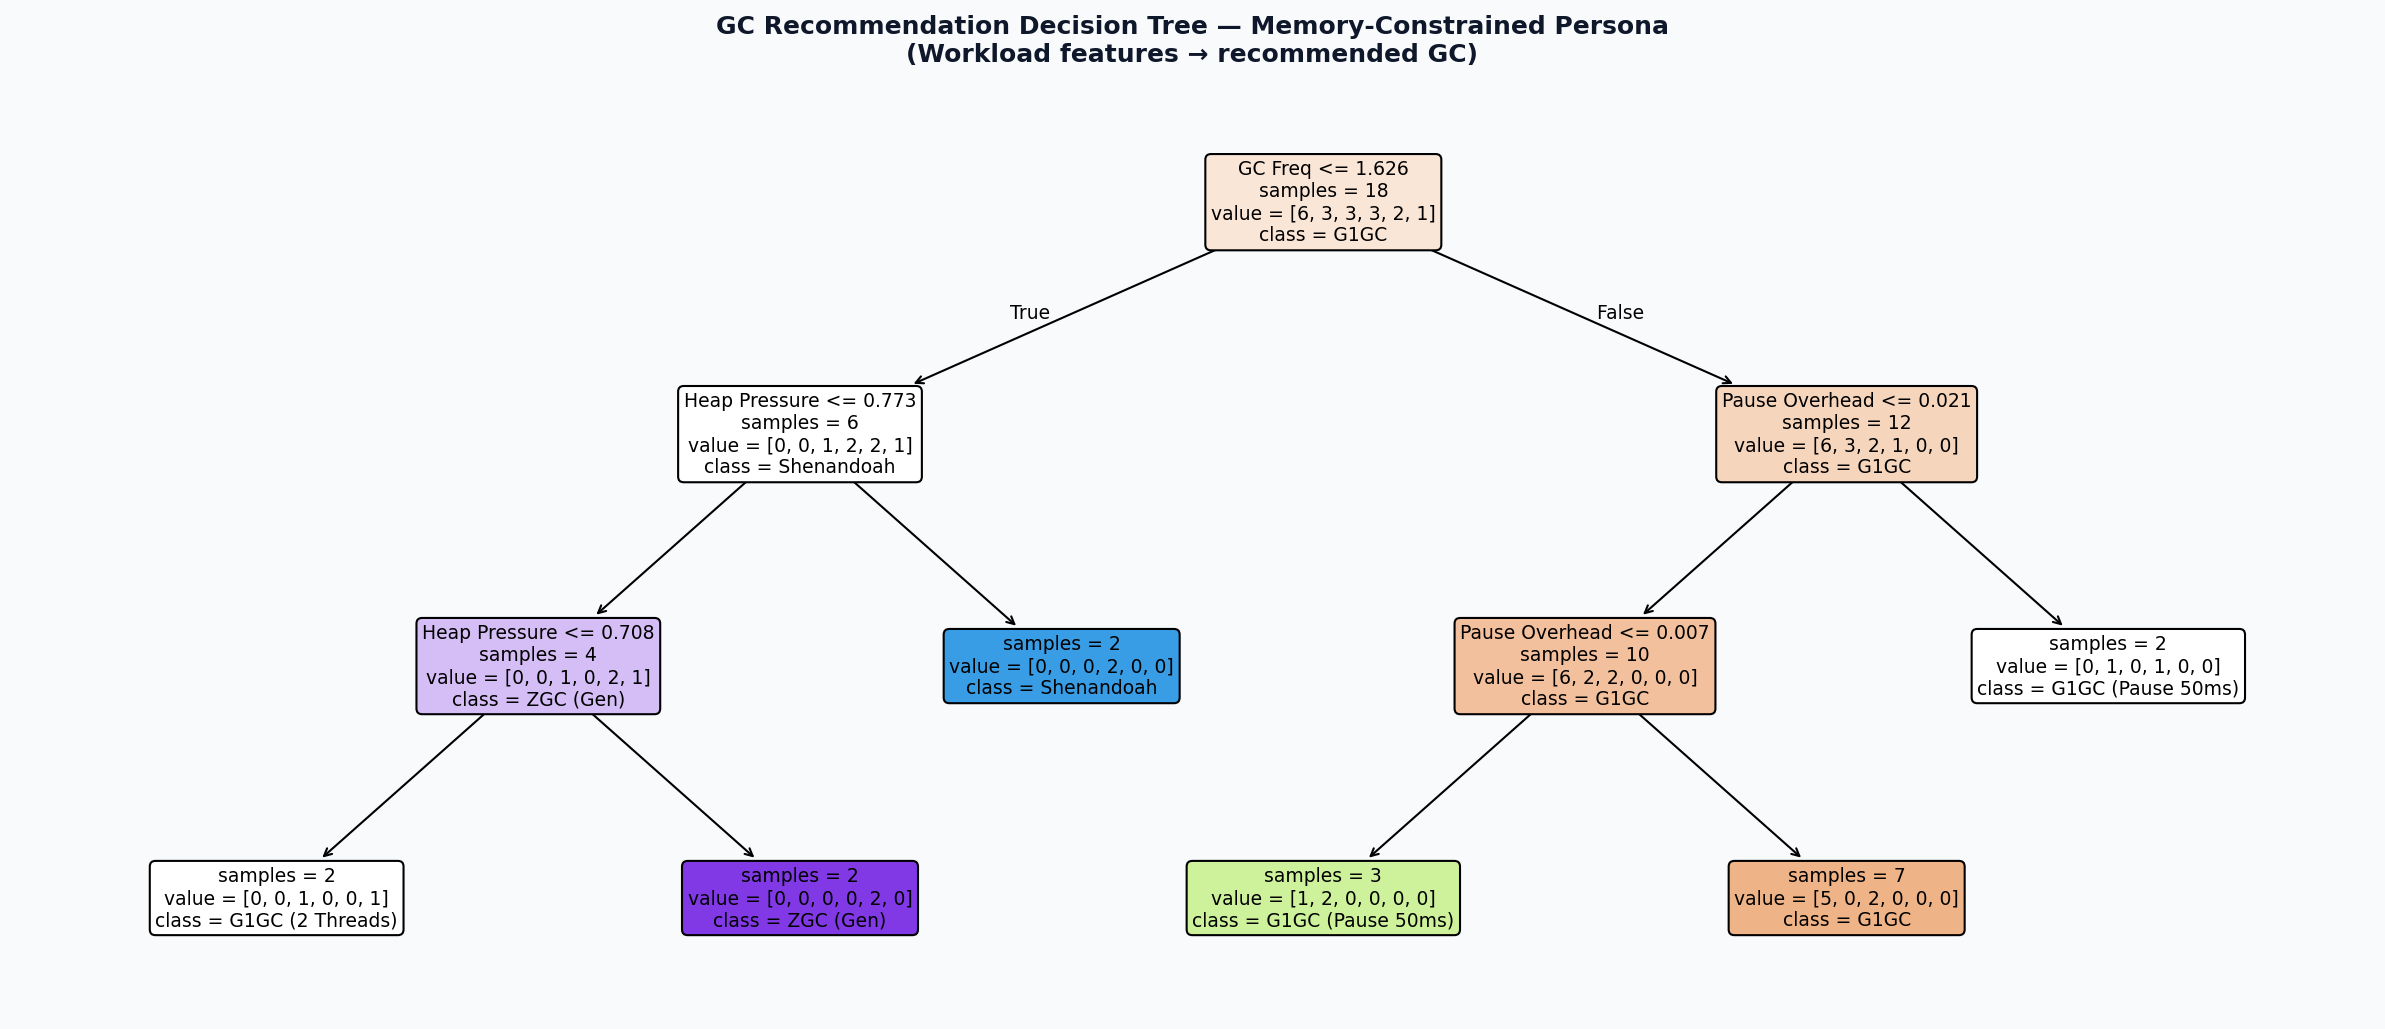
\includegraphics[width=\linewidth]{graphs/recommendation/decision_tree_memory_constrained.png}
\caption{Decision Tree (Memory Constrained)}
\end{subfigure} &
\begin{subfigure}{0.45\textwidth}
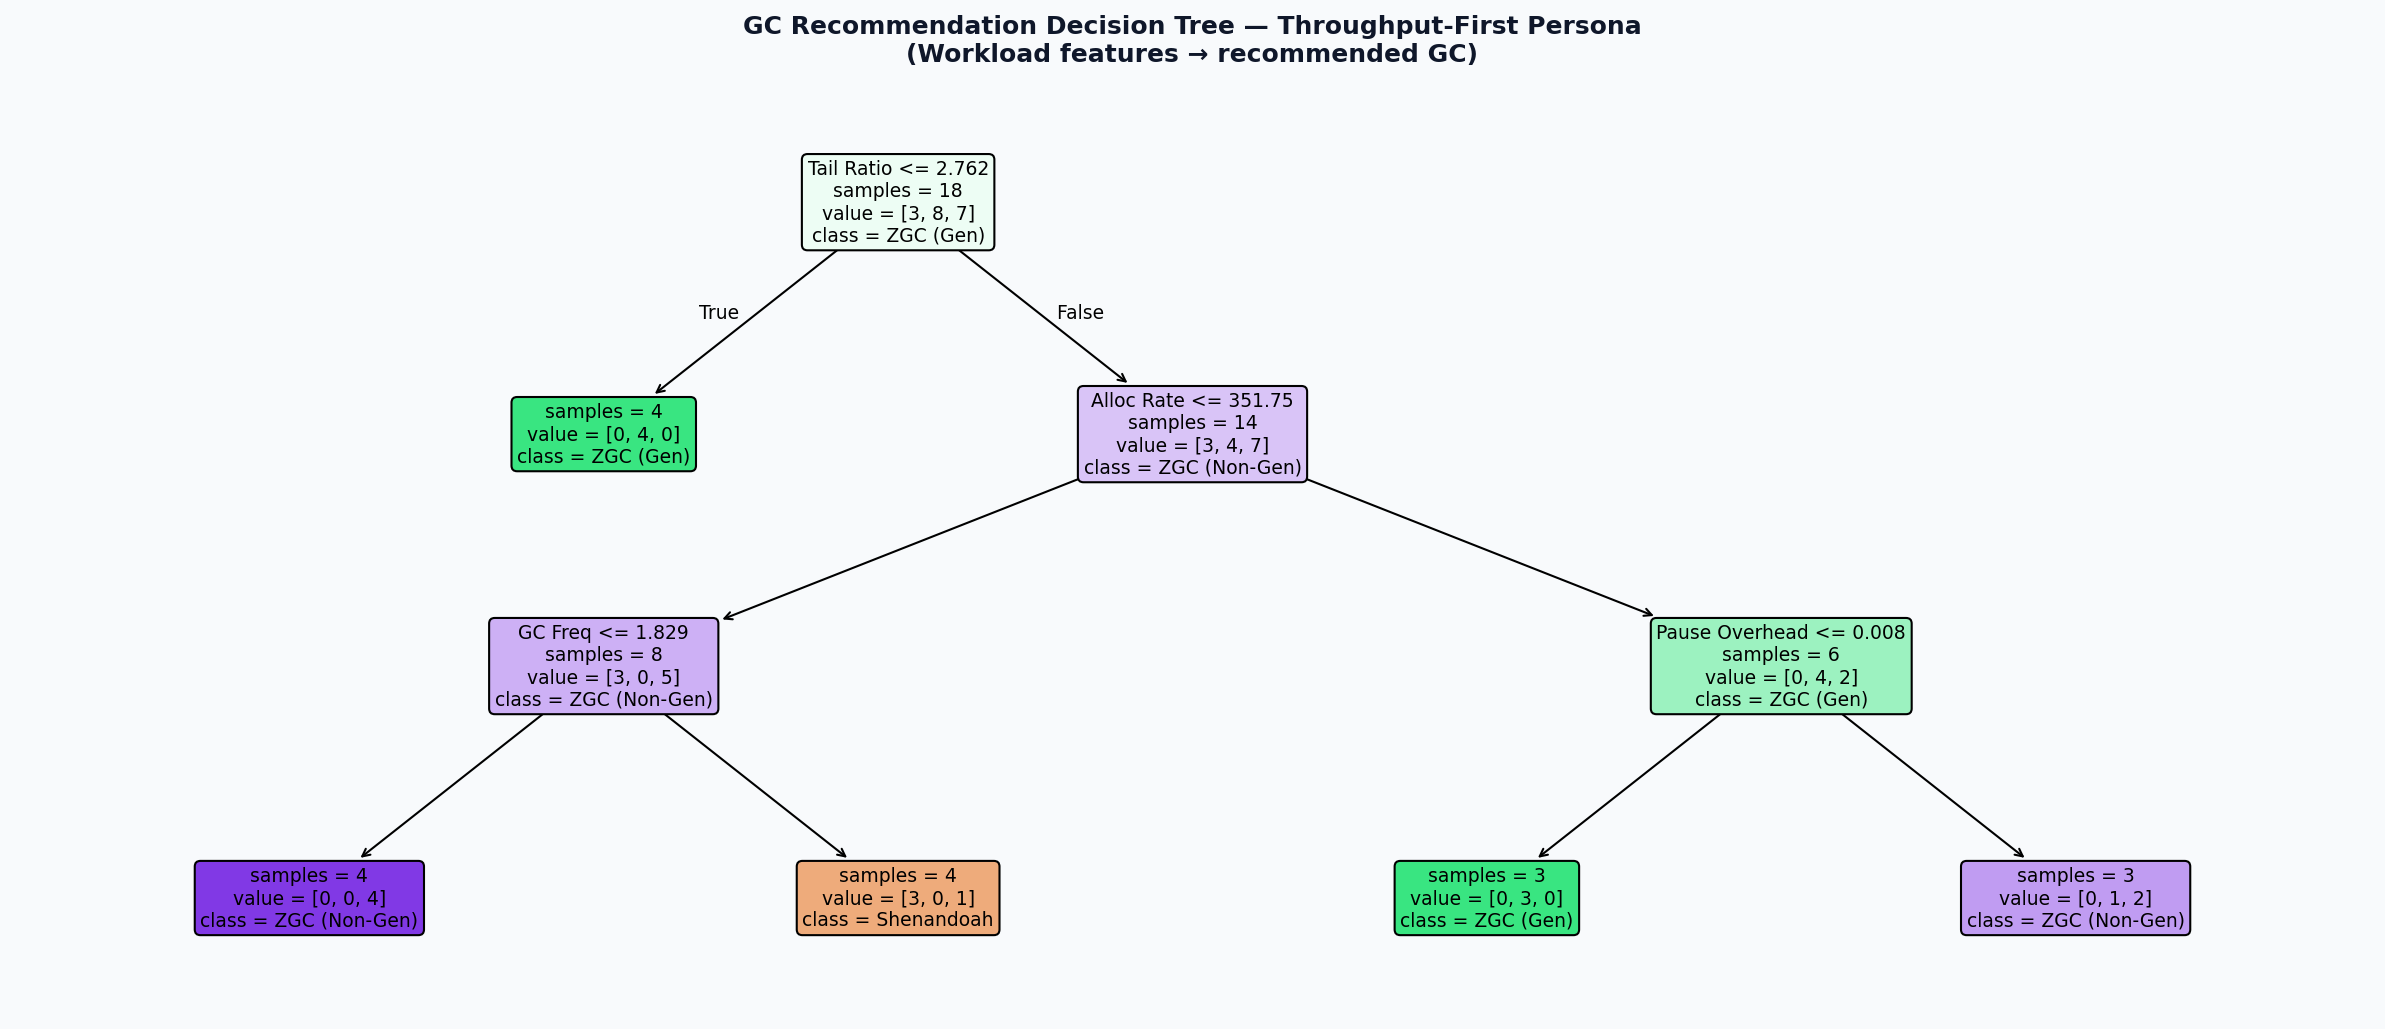
\includegraphics[width=\linewidth]{graphs/recommendation/decision_tree_throughput_first.png}
\caption{Decision Tree (Throughput First)}
\end{subfigure} \\

\begin{subfigure}{0.45\textwidth}
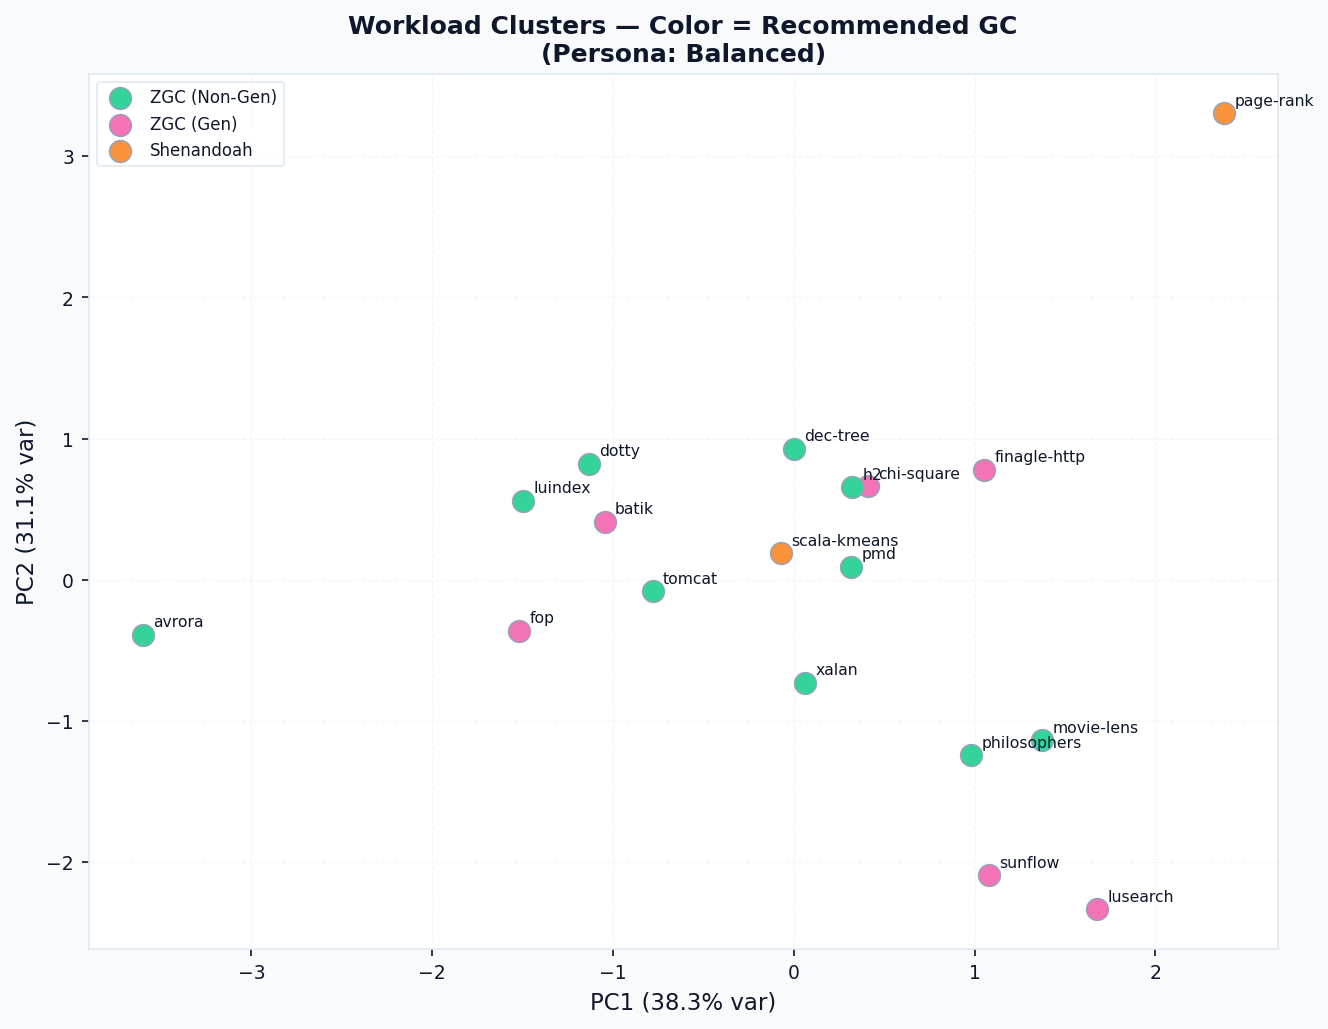
\includegraphics[width=\linewidth]{graphs/recommendation/pca_cluster_balanced.png}
\caption{PCA Cluster (Balanced)}
\end{subfigure} &
\begin{subfigure}{0.45\textwidth}
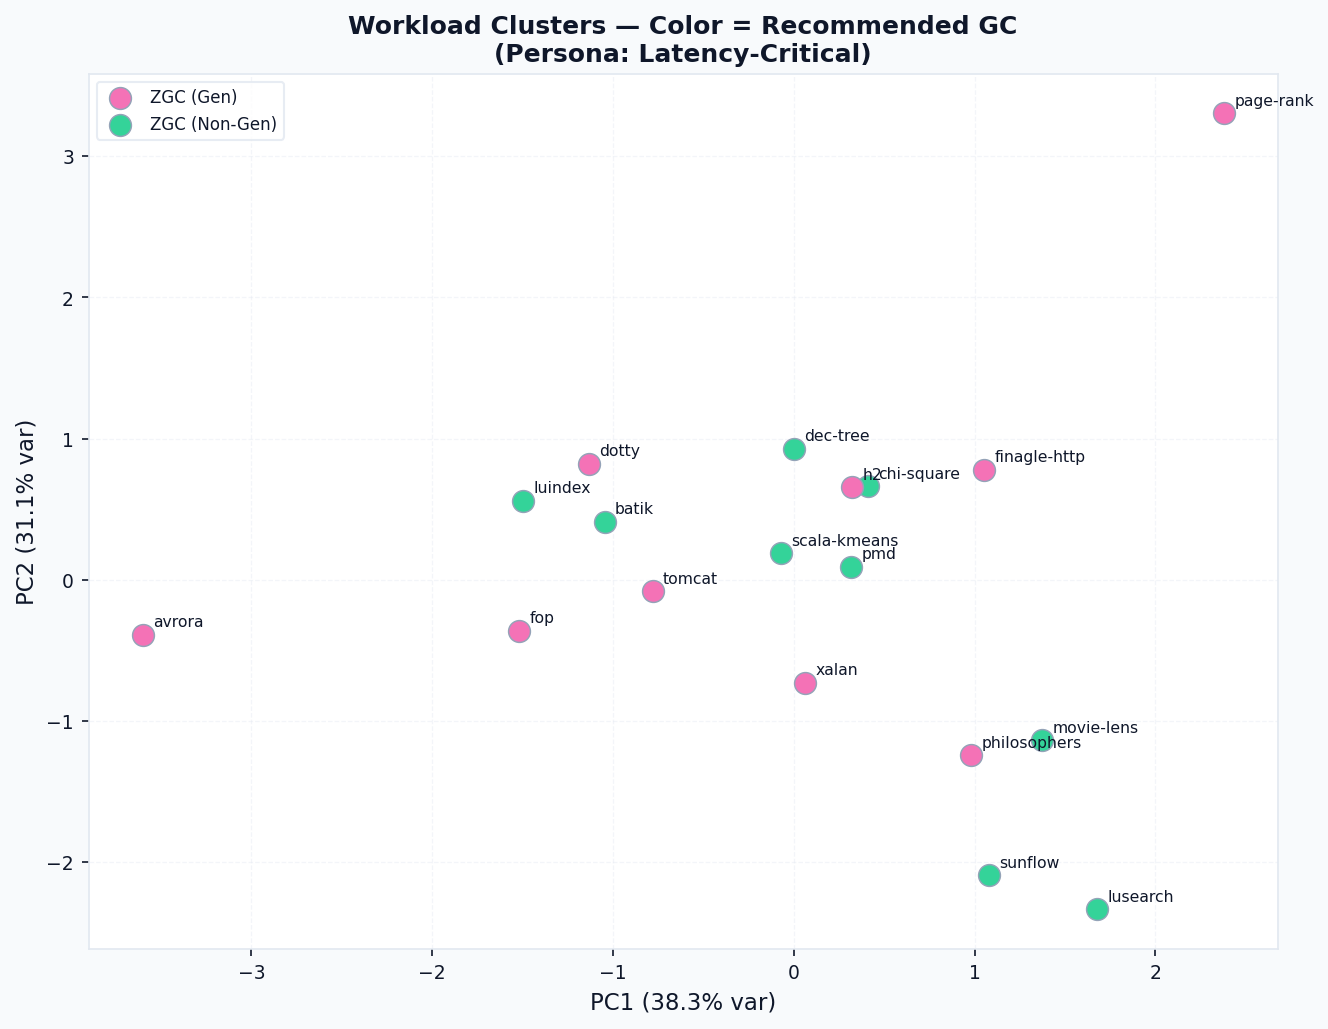
\includegraphics[width=\linewidth]{graphs/recommendation/pca_cluster_latency_critical.png}
\caption{PCA Cluster (Latency Critical)}
\end{subfigure} \\

\begin{subfigure}{0.45\textwidth}
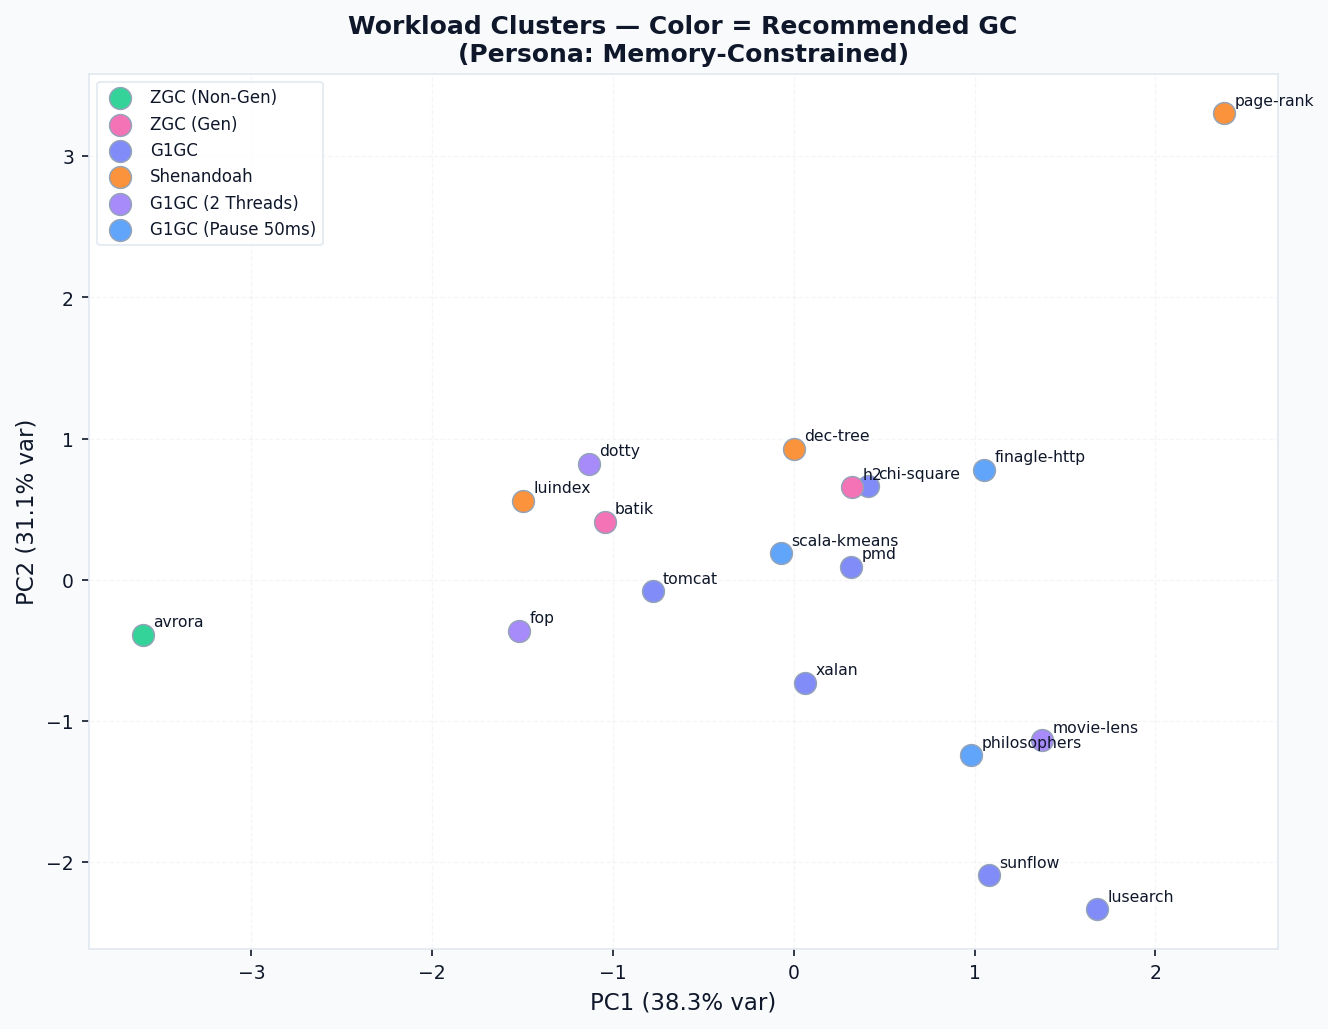
\includegraphics[width=\linewidth]{graphs/recommendation/pca_cluster_memory_constrained.png}
\caption{PCA Cluster (Memory Constrained)}
\end{subfigure} &
\begin{subfigure}{0.45\textwidth}
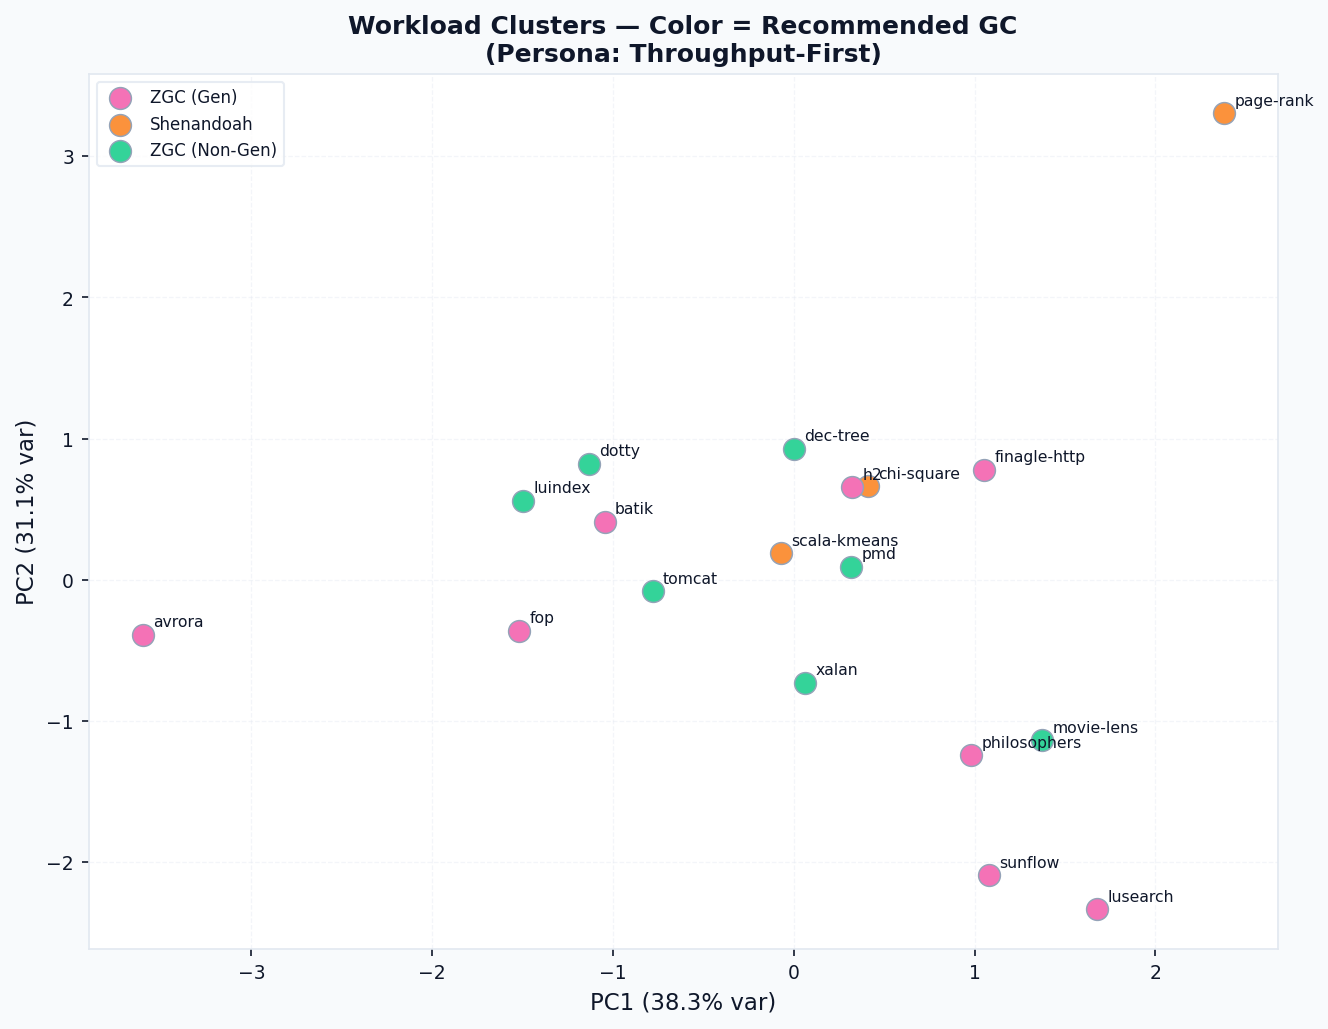
\includegraphics[width=\linewidth]{graphs/recommendation/pca_cluster_throughput_first.png}
\caption{PCA Cluster (Throughput First)}
\end{subfigure} \\

\end{tabular}

\caption{Garbage Collector Recommendation Models using Decision Tree and PCA Clustering under Different Scenarios}
\label{fig:gc_recommendation}
\end{figure}

